%% 
%% This is a sample doctoral dissertation.  It shows the appropriate
%% structure for your dissertation.  It should handle most of the
%% strange requirements imposed by the Grad school; like the different
%% handling of titles of one/many appendices.  It will automatically
%% handle the linespacing changes.  The body default is double-spaced
%% (except when you use the singlespace or condensed options).  The
%% default for quotations is single-space, and the default for tabular
%% environments is also single-space.  
%%
%% This class adds the following commands and environments to the
%% report class, upon which it is based:
%% Commands
%% ------------
%% \degree{name}{abbrv} -- Sets the name and abbreviation for the degree.
%%                         These default to ``Doctor of Philosopy''
%%                         and ``Ph.D.'', respectively.
%% \copyrightyear{year} -- for the copyright page.
%% \bachelors{degree}{institution} -- for the abstract
%% \masters{degree}{institution}   --  "
%%     if you have other degrees you may use
%% \secondbachelors{degree}{institution}
%% \thirdbachelors{degree}{institution}
%% \secondmasters{degree}{institution}
%% \thirdmasters{degree}{institution}
%% \priordoctorate{degree}{institution}
%%
%% \committeechair{name}           -- for the signature page
%% or, if you have two co-chairs:
%% \cochairs{first name}{second name}
%%
%% \firstreader{name}              --  "
%% \secondreader{name}             --  "
%% \thirdreader{name}              -- (optional)
%% \fourthreader{name}             --  "
%% \fifthreader{name}              --  "
%% \sixthreader{name}              --  "
%% \departmentchair{name}          -- for the signature page
%% \departmentname{name}           --  "
%%
%% \copyrightpage                  -- produces the copyright page
%% \signaturepage                  -- produces the signature page
%%
%% \frontmatter                    -- these are required in their various
%% \mainmatter                     -- appropriate locations
%% \backmatter                     --
%%
%% \unnumberedchapter[toc]{name}   -- like \chapter, except that it
%%                                    produces an unnumbered chapter;
%%                                    alternatively, like \chapter*,
%%                                    except that it lists the chapter
%%                                    in the table of contents.
%%
%% New environments:
%%   dedication  -- for the dedication
%%   abstract    -- for the abstract
%%
%% The thesis documentclass is built on top of the report document class.
%% It accepts all of the options that the report class accepts, plus the
%% following:
%%     doublespace -- the default, indicates double spacing as per U.Mass.
%%                    requirements.  You will need this when you do your
%%                    final copy.
%%     singlespace -- for earlier work, not acceptable to the Grad school
%%     condensed   -- for earlier work, not acceptable to the Grad school,
%%                    creates condensed versions of the frontmatter. 
%%                    Condensed implies singlespace.
%%     dissertation - the default, indicates that this document is a
%%                    dissertation.
%%     proposal    -- indicates that this document is a dissertation proposal,
%%                    rather than a dissertation.  This will only change the
%%                    wording on the title and signature pages.
%%     thesis      -- indicates that this document is a Master's thesis 
%%                    rather than a doctoral dissertation.  This also changes
%%                    the default for \degree to Master of Science, M.S.
%%     allowlisthypenation -- (the default), allows hyphenation of words in
%%                    the table of contents, the list of figures, and the list
%%                    of tables.  I believe that this is acceptable to the 
%%                    Graduate School.
%%     nolisthyphenation -- disallows hyphenation of words in the table of
%%                    contents and the list of figures and tables.  Use this 
%%                    option if the Grad School doesn't like your hyphenation.
%%     nicerdraft  -- relaxes some of the Grad School's rules for working with
%%                    drafts -- has no effect when doublespace is in effect
%%     nonicerdraft -- the default, leaves things in draft as they will be in
%%                     the final version
%% umassthesis changes the default font size to 12pt, but you may specify 10pt or
%%   11pt in the options.
\documentclass[dissertation]{umassthesis}          % for Ph.D. dissertation or proposal
\usepackage{xcolor}
\usepackage{float}
\usepackage{amsmath}
\usepackage{amssymb}
\usepackage[hidelinks]{hyperref}
\usepackage{graphicx}
\usepackage{booktabs}
\usepackage{multirow}
\usepackage{soul}

\usepackage[style=apa,backend=biber,uniquename=false,maxcitenames=2,maxbibnames=99]{biblatex}
\addbibresource{Papers.bib}
\begin{document}
% \documentclass[thesis]{umassthesis}  % for Master's thesis

%%
%% If you have enough figures or tables that you run out of space for their
%% numbers in the List of Tables or List of figures, you can use the following
%% command to adjust the space left for numbers.  The default is shown:
%%
%% \setlength{\tablenumberwidth}{2.3em}

%% Use the hyperref package if you're producing a version for online
%% distribution and you want hyperlinks.  Note that the Grad School doesn't want
%% their PDF viewers to colorize or otherwise highlight the links; use the
%% hidelinks option to hyperref to avoid decorating links.
%\usepackage[hidelinks]{hyperref}

%% One way of formatting the epigraph/frontispiece is to use this package.
%\usepackage{epigraph}

%%
%% You must fill in all of these appropriately
\title{Context dependence in perceptual and preferential choice}
\author{Sean Patrick Conway}
\date{September 2025} % The date you'll actually graduate -- must be
                     % February, May, or September
\copyrightyear{2025}
\bachelors{B.A.}{University of Wisconsin-La Crosse}
\masters{M.S.}{University of Wisconsin-Oshkosh}

\committeechair{Andrew L. Cohen}
\firstreader{Youngbin Kwak}
\secondreader{Elizabeth Miller}
\thirdreader{Jeffrey Starns}

\departmentchair[Department Chair]{Ilia Karatsoreos} 
\departmentname{Psychological and Brain Sciences}

\degree{Doctor of Philosopy}

%%
%% These lines produce the title, copyright, and signature pages.
%% They are Mandatory; except that you could leave out the copyright page
%% if you were preparing an M.S. thesis instead of a PhD dissertation.
\frontmatter
\maketitle
\copyrightpage     %% not required for an M.S. thesis
\signaturepage

%%
%% Dedication is optional -- but this is how you create it
%\begin{dedication}              % Dedication page
%  \begin{center}
%    \emph{To those little lost sheep.}
%  \end{center}
%\end{dedication}

%%
%% Epigraph (aka frontispiece) is also optional, but this is one way you
%% can create it
%\begin{frontispiece}
%  %% Format to your liking -- see documentation of epigraph package
%  \setlength{\epigraphrule}{0pt}
%
%  \begin{epigraphs}
%    \qitem{%
%      \itshape
%      Mary had a little lamb,\\
%      Her fleece was white as snow.\\
%      \vspace{\baselineskip}
%      And everywhere that Mary went\\
%      The lamb was sure to go.
%      \vspace{\baselineskip}}
%    {Sarah Josepha Hale}
%
%    \vspace{2\baselineskip}
%    \qitem{%
%      \itshape
%      Baa, baa, black sheep,\\
%      Have you any wool?\\
%      Yes, sir, yes, sir,\\
%      Three bags full;\\
%      One for the master,\\
%      And one for the dame,\\
%      And one for the little boy\\
%      Who lives down the lane.
%      \vspace{\baselineskip}}
%    {English Nursery Rhyme}
%
%  \end{epigraphs}
%\end{frontispiece}

%%
%% Acknowledgements are optional...yeah, right.
%\chapter{Acknowledgments}             % Acknowledgements page
%Thank you to...

%%
%% Abstract is MANDATORY. -- Except for MS theses
\begin{abstract}  
A large body of research in psychology has shown that context can systematically affect choice These \textit{context effects} are in violation of rational choice theory and are both practically and theoretically interesting. Recent work has demonstrated context effects in simple perceptual choice,  findings that suggest that these results are not restricted to high-level (e.g., consumer) choice. This dissertation explores the attraction and repulsion effects, two related context effects, with a particular emphasis on perceptual choice. Chapter 1 introduces the attraction and repulsion effects and reviews the empirical and theoretical literature surrounding them. Chapter 2 tests the ability of perceptual and decisional processes to account for these effects via a Thurstonian choice model. Chapter 3 uses this model to make predicts about best-worst choice and test them empirically. Chapter 4 generalizes the Thurstonian model and experimental paradigm from Chapter 2 to consumer choice. Chapter 5 tests the idea that an effect similar to that of Chapter 2 can be generated through ease of inter-option comparability in perceptual choice. Chapter 6 summarizes and discusses these results.                   % Abstract
\end{abstract}

%%
%% Preface goes here...would be just like Acknowledgements -- optional
%% \chapter{Preface} 
%% ...


%%
%% Table of contents is mandatory, lists of tables and figures are 
%% mandatory if you have any tables or figures; must be in this order.
\tableofcontents                % Table of contents
\listoftables                   % List of Tables
\listoffigures                  % List of Figures

%%
%% I don't handle List of Abbreviations
%% I don't handle Glossary

%%%%%%%%%%%%%%%%%%%%%%%%%%%%%%%%%%%%%%%%%%%%%%%%%%%%%%%%%%%%%%%%%%%%%%%%%
%% Time for the body of the dissertation
\mainmatter   %% <-- This line is mandatory

%%
%% If you want an introduction, which is not a numbered chapter, insert
%% the following two lines.  This is OPTIONAL:
%\unnumberedchapter{Introduction}


%%
%% Some sample text
\chapter{Introduction}
\label{introduction}
\section{Overview}
% Researchers universally assume that participants use the input they receive (i.e., the value of each option) to make a choice.
Decades of decision-making research have shown that context can systematically affect choice. In decision-making experiments, researchers present participants with a finite set of options on each trial and ask them to select a single option based on either an internal (e.g., most preferable) or external (e.g., largest shape) criterion. Decision-making research spans multiple fields, including psychology, neuroscience, economics, marketing, and political science. In economics, for example, researchers have developed models based on the idea that, while preferences may vary from moment to moment, people generally make rational choices in any given choice setting. In psychology and marketing, however, researchers have identified a set of phenomena that violate such assumptions, by showing that choices can vary with the \textit{choice set}, or the menu of available options. This class of phenomena is known as \textit{context effects} .

Context effects are interesting to decision-making researchers because they violate properties of large classes of choice models, such as Independence of Irrelevant Alternatives (IIA) \parencite{ray1973independence} and regularity \parencite{mackay1995probabilistic,marley1989random}. IIA states that the likelihood of selecting one option over another is invariant of other options available. Regularity states that the probability an option is chosen cannot increase upon the addition of new options to a choice set. IIA and regularity are also properties of Luce's Choice Axiom, a highly influential model of stochastic choice \parencite{luceChoiceAxiomTwenty1977a, luce1959individual}. 

One notable context effect, the attraction effect, occurs when the choice share of a \textit{target} option increases upon the inclusion of a similar but inferior \textit{decoy} option \parencite{huberAddingAsymmetricallyDominated1982d}. Another finding, the repulsion effect, occurs when a decoy boosts the choice share of a dissimilar \textit{competitor} option rather than the target \parencite{simonson2014vices}. The repulsion effect is an empirical reversal of the attraction effect. 

Context effects, originally studied in preferential choice, have been recently demonstrated simple perceptual choice \parencite{trueblood2013not,spektorWhenGoodLooks2018b,liaoInfluenceDistanceDecoy2021,spektorRepulsionEffectPreferential2022,yearsleyContextEffectsSimilarity2022,truebloodPhantomDecoyEffect2017c, turnerCompetingTheoriesMultialternative2018a, evansImpactPresentationOrder2021}. This is theoretically interesting because it suggests that context effects are a theoretical primitive rather than simply a feature of high-level consumer choice \parencite{trueblood2013not}. 

As suggested by the title, this dissertation explores various forms of context dependence in both perceptual and preferential choice. In particular, I explore the attraction and repulsion effects. The goal of this dissertation is to understand how and why these the attraction and repulsion effects occur, by employing well-studied statistical models from the psychology literature. Additionally, this dissertation sets out to differentiate perceptual processes from decision-making processes in context effects (specifically, the attraction and repulsion effects).

As I will discuss throughout this dissertation but particularly in Chapter 2, recent work has demonstrated inconsistency in context effects, particularly in perceptual choice. I use behavioral experiments and statistical modeling in an attempt to reconcile these inconsistencies.

This dissertation is structured as follows. In Chapter 2, I develop and test a statistical model of perceptual variability when applied to context effects. In Experiment 1, I first show that the types of stimuli used in perceptual choice context effects experiments are easily confusable and vary systematically with theoretically relevant properties of the stimuli. In Experiment 2, I use the results of a high-powered psychophysics experiment to show that the repulsion effect, but not the attraction effect, is naturally predicted by this statistical model. In Chapter 3, I further test the statistical model by applying it to best-worst choice. In Chapter 4, I generalize the paradigm and model to preferential choice. Finally, in Chapter 5, I use a perceptual choice experiment to show that stimulus comparability affects choice, even when the decoy is equally similar to both focal options. In Chapter 6, I summarize the findings of the dissertation, their implications, and discuss future directions for research in this domain. 


\chapter{Parsing the Roles of Perception and Decision in Context-Dependent Choice}
\label{chapter_2}
\section{Introduction}

As discussed in Chapter 1, the attraction effect is a well-studied choice phenomenon where an asymmetrically dominated decoy option increases the choice share of a similar target option \parencite{huberAddingAsymmetricallyDominated1982d}. The attraction effect is an example of a context effect, where choice for an option varies systematically with choice set.

In recent years, researchers have extended context effect research to perceptual choice. \textcite{trueblood2013not} demonstrated the attraction effect in perceptual choice. In their experiments, participants saw three rectangles on each trial, arranged in a horizontal array, and selected the option they perceived to have the largest area. See see Figure~\ref{fig:fig_opts} (right panel).  Options $A$ and $B$ have equal area but trade off in height and width. \footnote{\textcite{trueblood2013not} also demonstrated the similarity and compromise effects.} Notably, the title of their paper was "Not Just for Consumers: Context Effects Are Fundamental to Decision Making", and in their General Discussion, \textcite{trueblood2013not} argued "our experiments suggest that these context effects are a general feature of human choice behavior because they are a fundamental part of decision-making processes. As such, our results challenge explanations of these effects exclusively in terms that are unique to high-level decision making and thus call for a common theoretical explanation that applies across paradigms." (p. 907). According to \textcite{trueblood2013not}, context effects are not idiosyncratic to high-level choices but are a fundamental feature of choice. \textcite{trueblood2013not} also used these perceptual results to argue against the context-dependent advantage (CDA) model developed by \textcite{tversky1993context} as well as the Leaky Competing Accumulators model of \textcite{usherLossAversionInhibition2004a}, as these models use loss aversion (the idea that an option's disadvantages on an attribute are weighted more strongly than its advantages on other attributes) to account for context effects \parencite[~see also]{truebloodPhantomDecoyEffect2017c}. \textcite{truebloodMultialternativeContextEffects2012} demonstrated context effects in an inference task and argued similarly against loss aversion as a mechanism for context effects. 

\textcite{turnerCompetingTheoriesMultialternative2018a} replicated \textcite{trueblood2013not}'s results and performed a large scale modeling study, comparing the ability of numerous mechanisms assumed by decision models to account for context effects. For example, \textcite{turnerCompetingTheoriesMultialternative2018a} concluded that pairwise comparisons on individual attributes greatly improves models' ability to account for context effects. This may not be appropriate, however, given a perceptual domain where dimensions may not be separable \parencite{ashbyVarietiesPerceptualIndependence1986a}. 

\textcite{spektorWhenGoodLooks2018b} followed up on this work and demonstrated the \textit{repulsion effect} in a rectangle choice experiment. In the repulsion effect, the competitor's choice share is higher than the target's choice share \parencite{liaoInfluenceDistanceDecoy2021,evansImpactPresentationOrder2021,simonsonVicesVirtuesMisguided2014,frederickLimitsAttraction2014b,spektorRepulsionEffectPreferential2022,banerjeeFactorsThatPromote2024,bhui2021rational}. In \textcite{spektorWhenGoodLooks2018b}'s experiments, the target and competitor options varied in area, such that one option was always larger, but on average they were the same size. The researchers also varied the \textit{target-decoy attribute distance} (TDD), the percentage difference between the target and decoy areas. For example, if TDD is $2\%$, the decoy is $2\%$ smaller than the target. 

\begin{figure}
   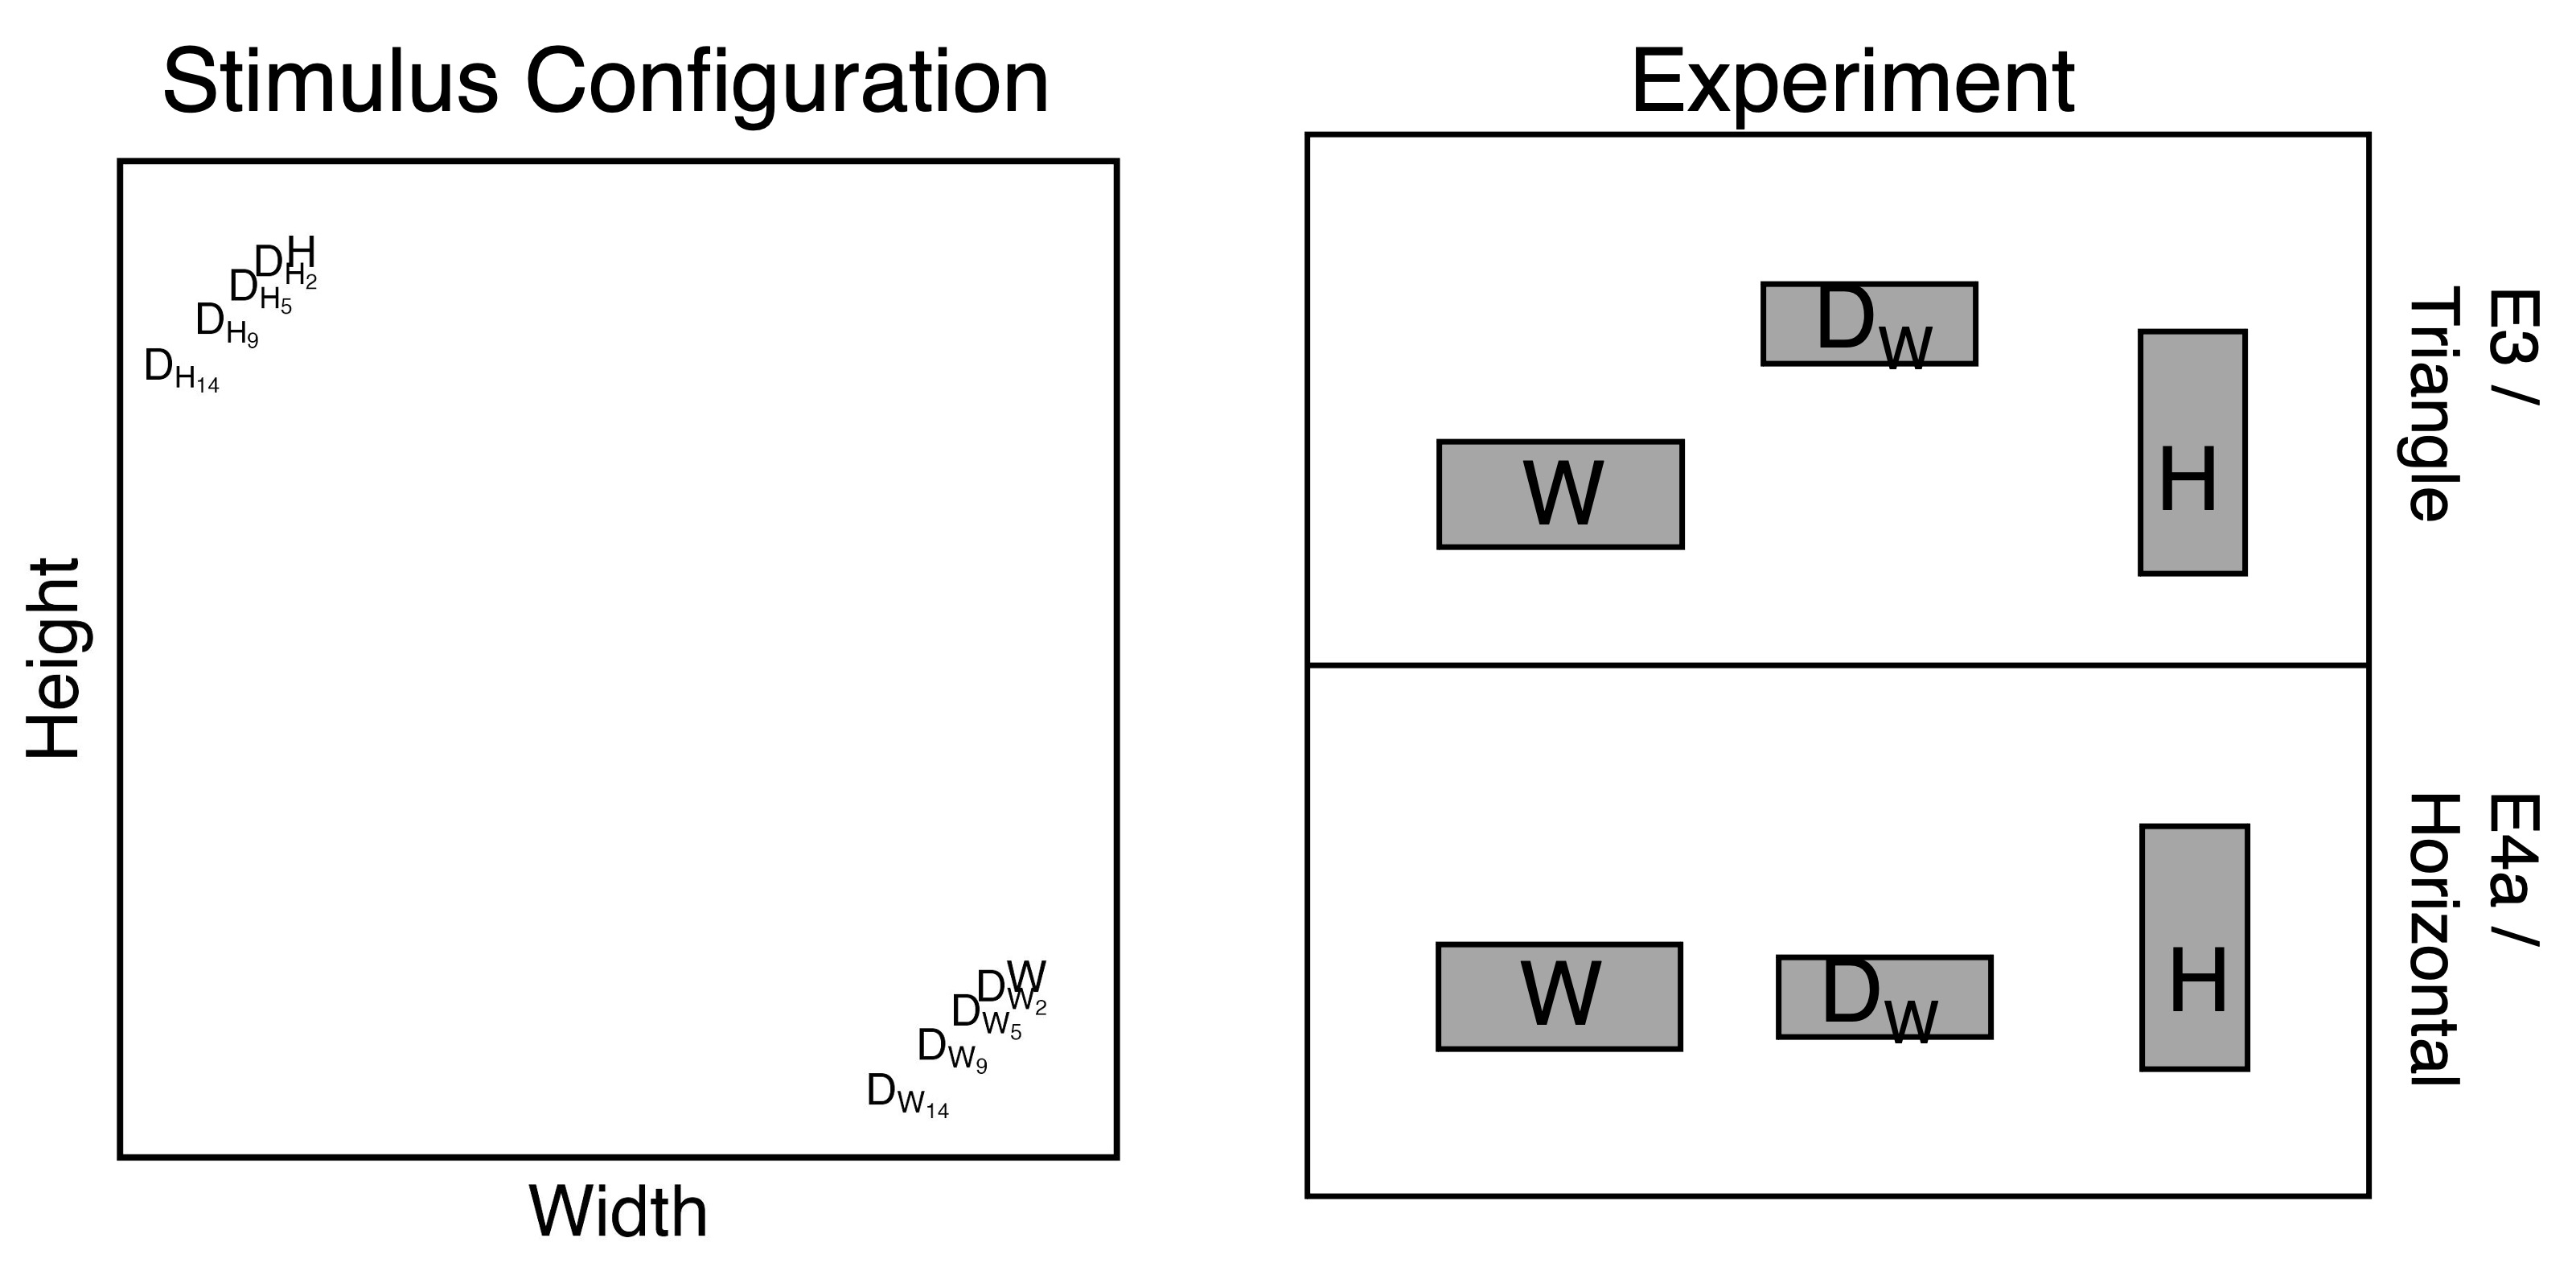
\includegraphics[width=\linewidth]{figures/spektor_stim.png}
   \caption{Stimulus configuration and example trials from \textcite{spektorWhenGoodLooks2018b}, Experiments 3 and 4a.}
   \label{fig:spektor_stim}
\end{figure}

\textcite{spektorWhenGoodLooks2018b} ran a total of five experiments. All experiments showed similar results, so I focus on their experiments 3 and 4a, which are the most representative of the article's conclusions. In Experiment 3, the authors varied TDD at four levels: $2\%$, $5\%$, $9\%$, and $14\%$. The rectangles were arranged in a trianglular display on the screen (see Figure~\ref{fig:spektor_stim}, Experiment 3), in contrast to \textcite{trueblood2013not}'s horizontal display. \textcite{spektorWhenGoodLooks2018b} found an empirical repulsion effect such that the competitor was selected more than the target at all levels of TDD (see Figure~\ref{fig:spektor_stim}). 

\textcite{spektorWhenGoodLooks2018b} also ran a follow-up experiment using the horizontal diplay of \textcite{trueblood2013not} (see Figure~\ref{fig:spektor_stim}, Experiment 4a). Here, they varied TDD at $5\%$, $9\%$, and $14\%$. In Experiment 4a, the data show a slight repulsion effect at low TDD levels that eventually becomes an attraction effect at high TDD levels. 

\textcite{truebloodPhantomDecoyEffect2017c} demonstrated a "phantom decoy" effect in perceptual choice. Phantom decoys are options that are similar to the target, but also superior in value, and are presented but made unavailable at the time of choice. They showed that participants chose the target less than the competitor, i.e., a repulsion effect, a result at odds with phantom decoy effects in preferential choice \parencite{pratkanisBriefHistoryResearch1992b,pettiboneExaminingModelsNondominated2000}. 

\begin{figure}
   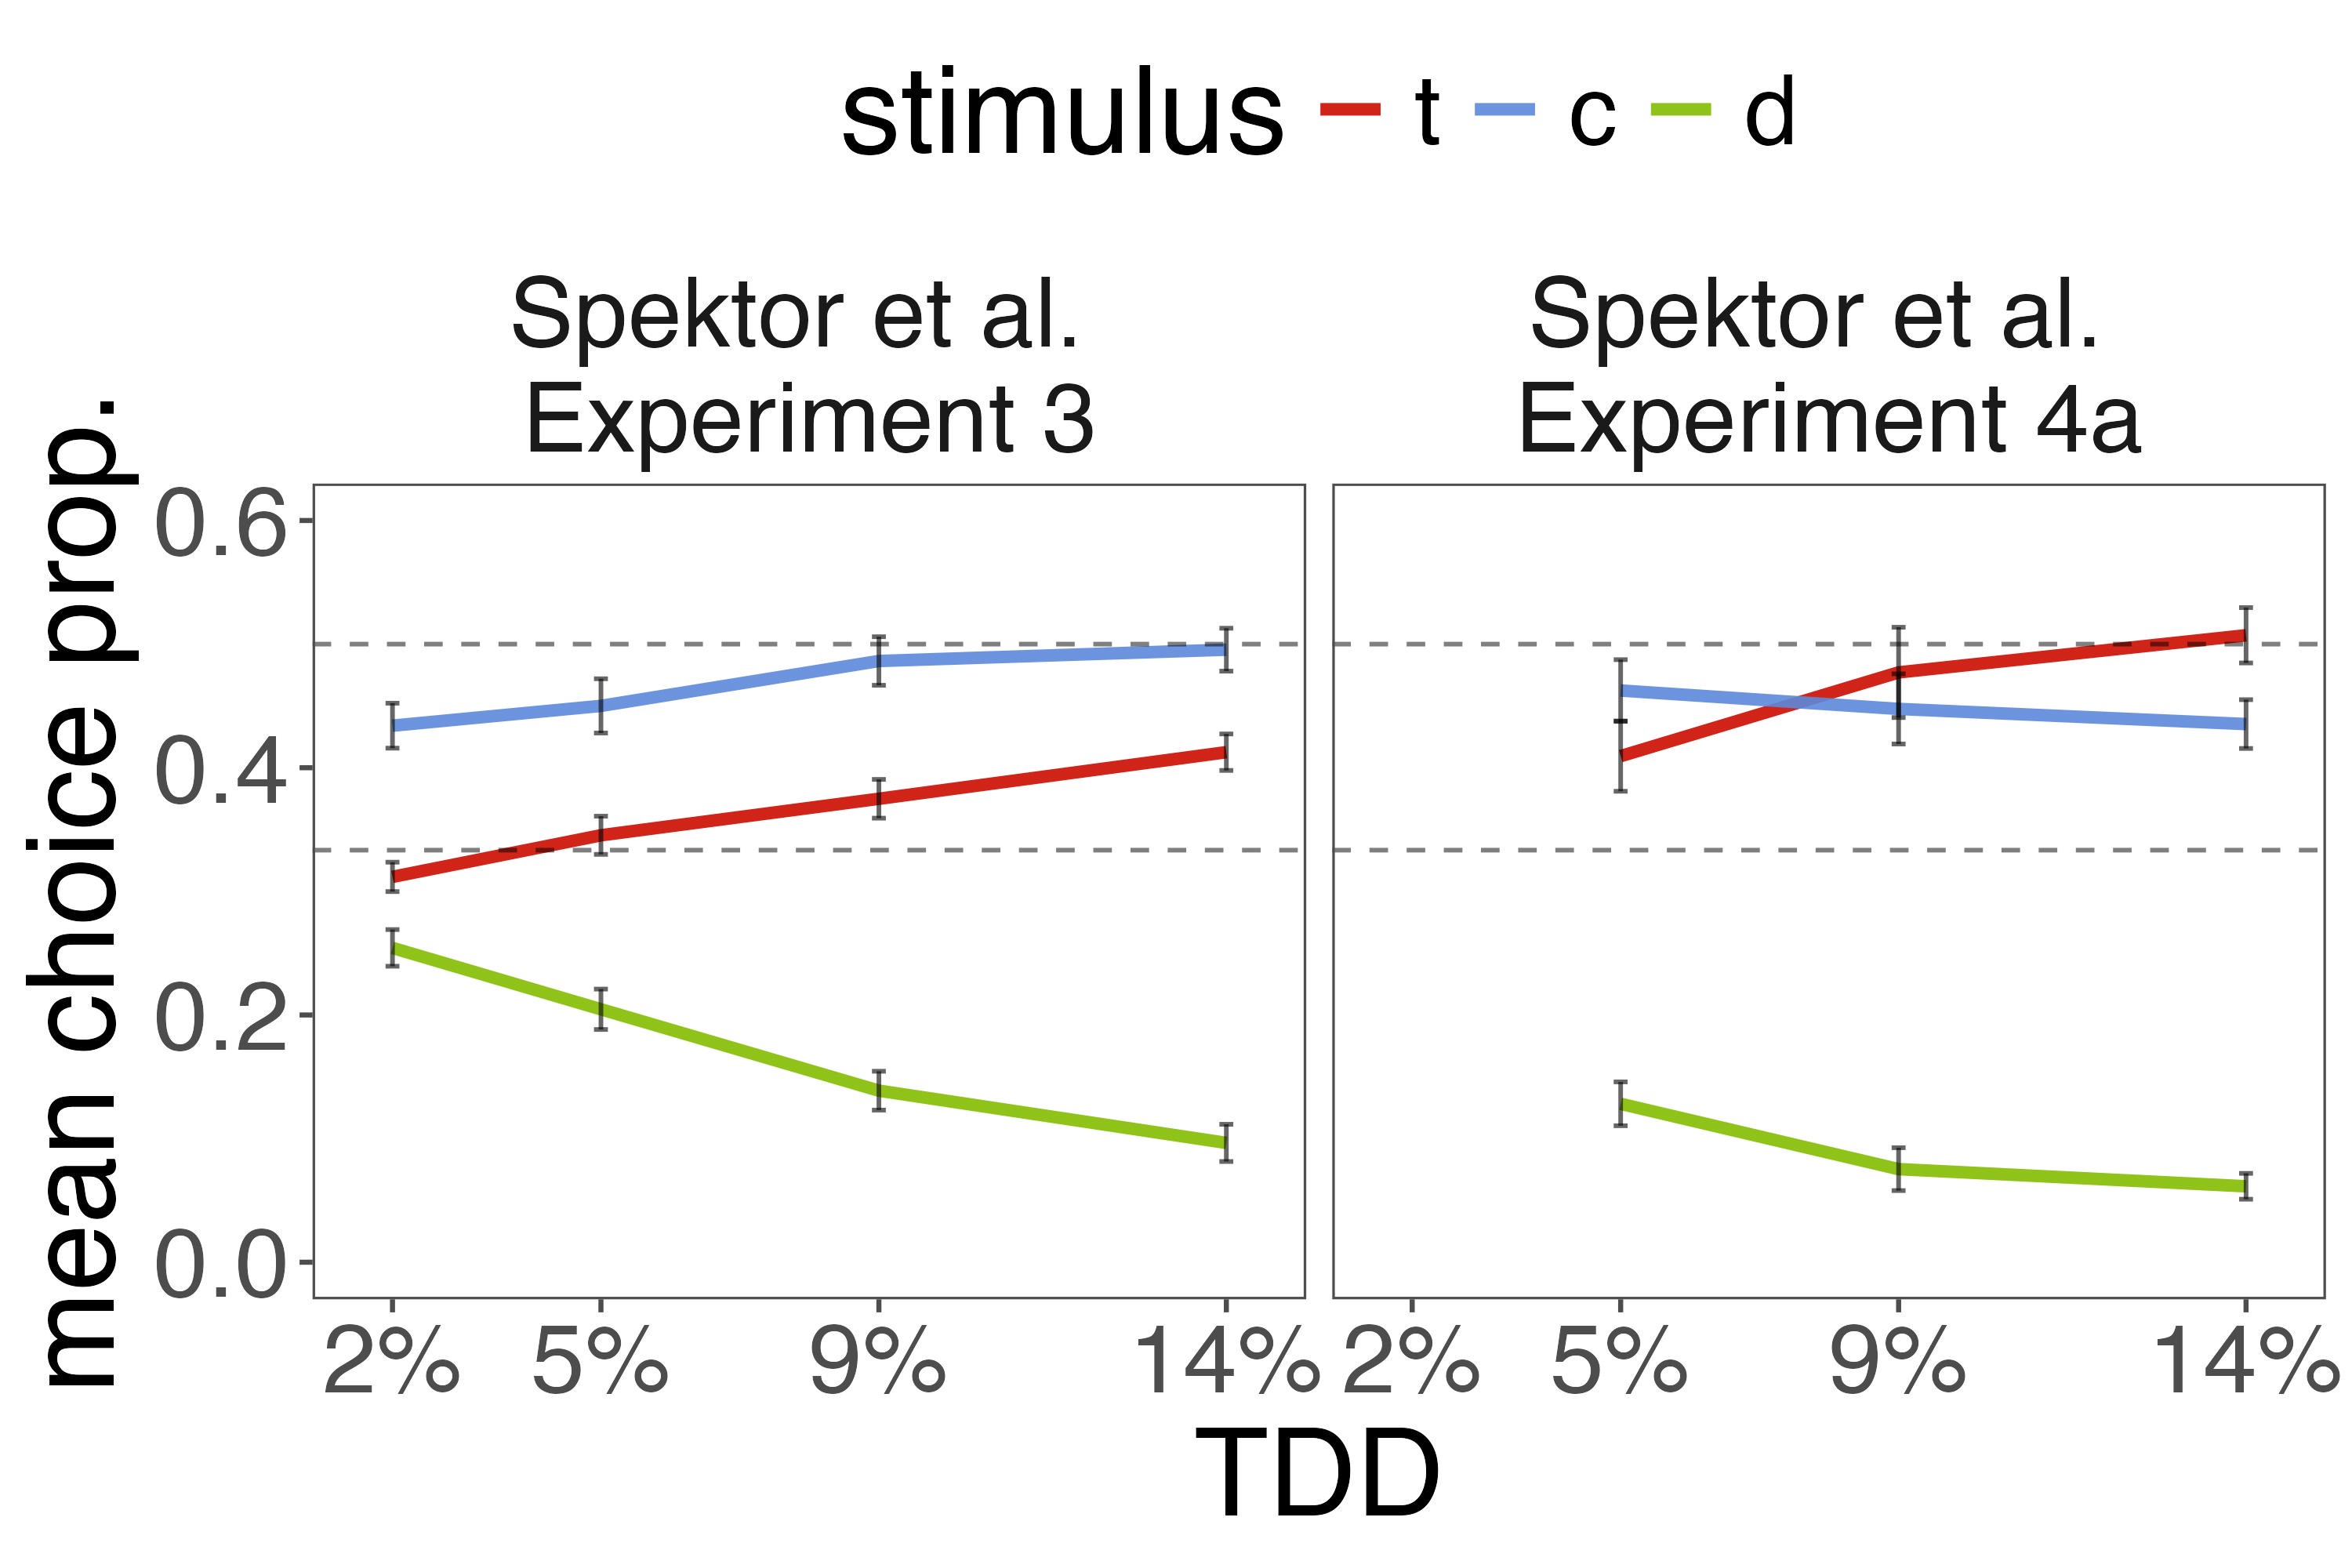
\includegraphics[width=\linewidth]{figures/spektor_data_collapsed.jpeg}
   \caption{Data from \textcite{spektorWhenGoodLooks2018b}, collapsed across choice set. Error bars are $95\%$ CIs of the mean, computed using the within-subjects error correction from \textcite{morey2008confidence}. Dashed lines are drawn at .5 and .33.}
   \label{fig:spektor_data} % might consider graphing (or at least writing RSTs) here
\end{figure}

\textcite{liaoInfluenceDistanceDecoy2021} also replicated the general pattern of \textcite{spektorWhenGoodLooks2018b}'s results and also found a an inverse U-shaped relationship between TDD and the \textit{Relative Share of the Target} RST\footnote{$RST=\frac{P(T|[T,C,D])}{P(T|[T,C,D)+P(C|[T,C,D])}$. $RST>.5$ indicates the attraction effect, while $RST<.5$ indicates the repulsion effec.t}. Relatively low and extremely high TDD values created a repulsion effect, while intermediate TDD values created an attraction effect. 

\textcite{spektorRepulsionEffectPreferential2022} demonstrated the repulsion effect in both preferential and perceptual choice, using similar stimuli and display configuration. In these experiments, the stimuli were various squares, each containing bars filled varying degrees with color. In perceptual choice, participants were to select the stimulus with the largest cumulative filled area. In the preferential choice scenario, participants were told that each filled bar represented one possible outcome of a 50-50 gamble, and they were to select the gamble with the highest expected value. Their results were similar to those of \textcite{spektorWhenGoodLooks2018b}, however, where target and competitor choices increased with TDD, with target and decoy showing a particularly strong trade-off.

Both \textcite{choplinComparisoninducedDecoyEffects2005b} and \textcite{yearsleyContextEffectsSimilarity2022} demonstrated the attraction effects in similarity judgments. In both sets of experiments, participants saw various perceptual stimuli (i.e., ovals, swirled lines, vertical lines) and chose the option most similar to a reference option. Both sets of researchers showed that dissimilar decoy options impacted participants' choices as in the attraction effect.

Researchers are clearly using perceptual experiments to demonstrate context effects and test theory. These results are clearly informative and theoretically interesting. I argue, however, that researchers should be cautious in assuming that decision-makers receive perceptual input with the same accuracy that they do in preferential choice experiments. Researchers should seek to separate the role of perceptual discriminability from decisional processes when understanding participants' responses. I elaborate on these ideas below and in Chapter 2, with a demonstration using the results of \textcite{spektorWhenGoodLooks2018b}.

\subsection{Understanding Perceptual Choice Experiments}

A crucial assumption made by researchers in the above experiments, is that participants are always (or almost always) to correctly perceive the target and competitor as larger than the decoy. This assumption is likely incorrect, as I will show empirically in Experimentn1. Furthermore, researchers assume that, to the extent that the dominance relationship is misperceived, the decoy is equally likely to be seen as larger than the target than larger than the competitor. 

One plausible account of \textcite{spektorWhenGoodLooks2018b}'s data is that participants occasionally misperceive the dominance relationship, and due to the difficulty of the task and the similarity of target and decoy, are more likely to choose the decoy over the target than the competitor. Such a process creates an empirical repulsion effect but is qualitatively different than a reversal of the traditional attraction effect. \textcite{spektorWhenGoodLooks2018b} dismiss such an account because the target is chosen more often the decoy; however, this fact does not rule out the above explanation of the data.

One goal of this dissertation is to separate the role of perceptual and decisonal processes in context effects. To do so, I begin with an extreme stance - that such experiments are solely perceptual experiments rather than decision-making experiments and that no high level decision processes are occurring. This extreme assumption is likely incorrect, but I believe it is a good place to start in understanding the existing data. I also demonstrate how and under what circumstances it is incorrect later in this dissertation. To begin, I return the results of \textcite{spektorWhenGoodLooks2018b}. 

As reported above, \textcite{spektorWhenGoodLooks2018b} demonstrate that a relatively small change in stimulus display (arranging stimuli in a triangle rather than a horizontal line) reverses the attraction effect. Why is this? To begin to answer this question, I highlight the differences between \textcite{spektorWhenGoodLooks2018b}'s data and previous context effect data. In preferential choice tasks, participants are given a set of options on each trial (e.g., laptops, apartments, washing machines), along with the attribute values associated with each option (e.g., 10 GB RAM, 1500 square feet, 2.7 cubic feet capacity). These attributes are typically represented numerically \parencite{hayes2024attribute,banerjeeFactorsThatPromote2024} or with easily discriminable graphical representations \parencite{cataldoComparisonProcessAccount2019b}. The decoy option, therefore, is rarely selected (e.g., $<5\%$ of all trials), and these selections are assumed to be the result of inattention or accidental responses. Researchers assume that participants are able to detect the dominance relationship between target and decoy. Perceptual choice tasks complicate participants' ability to detect this dominance relationship. In \textcite{spektorWhenGoodLooks2018b}'s experiments, the decoy is selected as often as $25\%$ of all trials in some conditions. The decoy is selected less often in experiment 4a (triangle display) than in experiment 3 (horizontal display). Decoy selections also decrease as the difference between decoy area and target/competitor areas increases. Finally, though both target and competitor increase in choice share as TDD increases, the target choice share increases at a higher rate than does the competitor, suggesting a strong trade-off between target and decoy choices (stronger, indeed, than that of competitor-decoy choices). That is, the mean \textit{Relative Share of the Target} (RST) \parencite{berkowitschRigorouslyTestingMultialternative2014b} increases with TDD in both experiments % should I explicitly show or write mean RST values? -Sean 1/9/25

Clearly, perceptual discriminability plays a role in \textcite{spektorWhenGoodLooks2018b}'s results. Participants clearly are better able to discriminate the target and competitor from the decoy as the decoy decreases in size. Any reasonable account of these data should parse the out discriminability from genuine context effects. 

There is a large body of psychological research, beginning with the work of \textcite{thurstone1927law}, of treating the perception of a stimulus as a random variable. In his famous "Law of Comparative Judgment" paper, \textcite{thurstone1927law} first showed that researchers can use binary choice proportions to estimate the psychological distance between stimuli, by treating perceptual intensity as a Gaussian random variable. This work led to similar research using Signal Detection Theory (SDT) \parencite{hautus2021detection}, which also treats psychological quantities (e.g., memory, perception), as random variables. Similarly, Ashby and colleagues' General Recognition Theory (GRT) models the perception of a stimulus as a multivariate normal random variable, where each dimension of the model is the perceived dimension of a stimulus \parencite{ashbyVarietiesPerceptualIndependence1986a,ashby1988decision, ashbyUnifiedTheorySimilarity}. In marketing and economics, researchers treat the utilities of choice options as random variables, which are often assumed to be Gaussian or Extreme Value Distributed and estimate choice models known as Random Utility Model (RUMs) \parencite{mcfadden2001economic,hausman1978conditional,train2009discrete}.Often, though not necessarily, these models share the common property that value (whether it is the utility of a consumer product, the perception of magnitude, or the memory signal in a recognition task) is stochastic while choice is deterministic  \parencite[~c.f.]{benjamin2009signal} 

\subsection{A Model of Context-Dependent Perceptual Choice}

I now introduce the model I explore throughout the dissertation.  This model is simplistic, as it treats the experiments of \textcite{trueblood2013not} and \textcite{spektorWhenGoodLooks2018b} as perceptual, rather than decision tasks. This also completely eschews the possibility of higher level decision processes. I use this model to differentiate perceptual from decision-making processes in the repulsion and attraction effects. The model treats value (perceived area) as stochastic and choice as deterministic. In the current modeling framework, I do not treat height and width as independent attributes but rather consider perceived area to be unidimensional. The model is set up to make predictions for a perceptual choice experiment, where participants are presented with 3 perceptual stimuli on each trial. I assume that on each trial $i$ with choice set $K$, The perception $\mathbf{X_i}$ of all 3 stimuli is sampled from a multivariate Gaussian distribution with a mean vector $\boldsymbol{\mu}$ and variance-covariance matrix $\boldsymbol{\Sigma}$:

\begin{align}
   \mathbf{X}_{i} \sim \mathcal{N}(\boldsymbol{\mu}, \boldsymbol{\Sigma})
   \label{eqn:mvnorm}
\end{align}

where $\boldsymbol{\mu}$ is a column vector consisting of:
\begin{align}
   \begin{pmatrix}
      \mu_{T} \\
      \mu_{C} \\
      \mu_{D}
      \end{pmatrix}
   \label{eqn:mu}
\end{align}

where the subscripts $T$, $C$, and $D$ indicate target, decoy, and competitor, respectively, and $\boldsymbol{\Sigma}$ is a positive semi-definite 3 x 3 covariance matrix computed as:

\begin{align}
   \boldsymbol{\Sigma}=S\boldsymbol{\Omega}S
   \label{eqn:Sigma}
\end{align}

where $S$ is a diagonal matrix consisting of: 

\begin{align}
   \begin{pmatrix}
      \sigma_{T} & 0 & 0 \\
      0 & \sigma_{C} & 0 \\
      0 & 0 & \sigma_{D} 
   \end{pmatrix}
\label{eqn:S}
\end{align}

with $\sigma_{T}$, $\sigma_{C}$, $\sigma_{D}$ being the standard deviations for target, competitor, and decoy, respectively. $\boldsymbol{\Omega}$ is a correlation matrix:

\begin{align}
   \begin{pmatrix}
      1 & \rho_{TC} & \rho_{TD} \\
      \rho_{TC} & 1 & \rho_{CD} \\
      \rho_{TD} & \rho_{CD} & 1 
   \end{pmatrix}
\label{eqn:O}
\end{align}
with $\rho_{TD}$, for example, indicating the population-level correlation between target and decoy stimuli.

As mentioned above, the model assumes that value is stochastic while choice is deterministic\footnote{This also assumes ties are not possible, which is true if and only if perceived area is absolutely continuous.}. The model always chooses the option perceived as largest, regardless of the magnitude of the difference between the "winner" and "runners-up". That is, given a vector $\mathbf{X}_i$ of perceived areas on trial $i$ with set $K$, the probability a participant selects stimulus $j$ is:

\begin{align}
   P(j|i,K)=P(\mathbf{X}_{ij}>\mathbf{X}_{ik}), j,k \in K, j \neq k
   \label{eqn:pchoice}
\end{align}

If all off-diagonal elements of $\boldsymbol{\Omega}$ are $0$, the model collapses to the standard Thurstonian Case V model \parencite{thurstone1927law} often used by cognitive psychology researchers. Models of this form have closed form solutions and their predictions are easy to compute.

On the other hand, if any elements of $\boldsymbol{\Omega}$ are non-zero, the closed form solution of this model does not exist, and to compute predictions and estimate model parameters, researchers must use simulation or numerical integration methods \parencite{train2009discrete}. In all applications of these model through this dissertation, I use simulation to generate model predictions. 

This model is capable of generating a(n) attraction (repulsion) effect by assuming $\mu_{T}>\mu_{C}$ ($\mu_{C}>\mu_{T}$), i.e., that on average target and competitor stimuli differ inherently in their perceived areas. This, however, is an ad hoc assumption that may describe the data well but will generate limited theoretical insight. Moreover, I wil later present empirical data in this dissertation that, generally speaking, $\mu_{T}=\mu_{C}$. 

I now consider the role of perceptual correlations between all pairs of stimuli, i.e., $\rho_{TC}$, $\rho_{TD}$, and $\rho_{CD}$. I vary both $\rho_{TD}$ and $\rho_{TC}$ from -1 to 1; in other words, all rectangles oriented the same way share one correlation and those oriented differently share another correlation. I show model predictions that result from varying these correlations in Figure~\ref{fig:3d_model}. Here, I assume that $\mu_{T}=\mu_{C}>\mu_{D}$ and that $\sigma_{T}=\sigma_{C}=\sigma_{D}$\footnote{In Experiment 2 I present evidence supporting these assumptions}. 

Figure~\ref{fig:3d_model} shows model predictions in the form of $RST$ (Relative Share of the Target), where RST values above .5 indicate an attraction effect and values below .5 indicate a repulsion effect. The model can, depending on the relationship between $\rho_{TD}$ and $\rho_{TC}$, predict a repulsion, attraction, or a null context effect. If $\rho_{TD}>\rho_{TC}$, the model predicts a repulsion effect. If the target and decoy are correlated more strongly than competitor and decoy, it is more likely that if on a particular trial the target perception is large, that the decoy is even \textit{larger}, causing the decoy to "steal" choice shares from the target more than the competitor, i.e., a repulsion effect.

If $\rho_{TD}<\rho_{TC}$, the model predicts an attraction effect. This is because $\rho_{TC}=\rho_{CD}>\rho_{TD}$, so the decoy "steals" choice shares from the competitor more than the target. 

Finally, if $\rho_{TD}=\rho_{TC}=\rho_{CD}$, the model predicts a null effect. In this case, no pair of stimuli are more correlated than any other pair, so the predictions are identical to a model where $\rho_{TD}=\rho_{TC}=\rho_{CD}=0$ model. This model collapses to an Independent Normal Model. 

\begin{figure}
   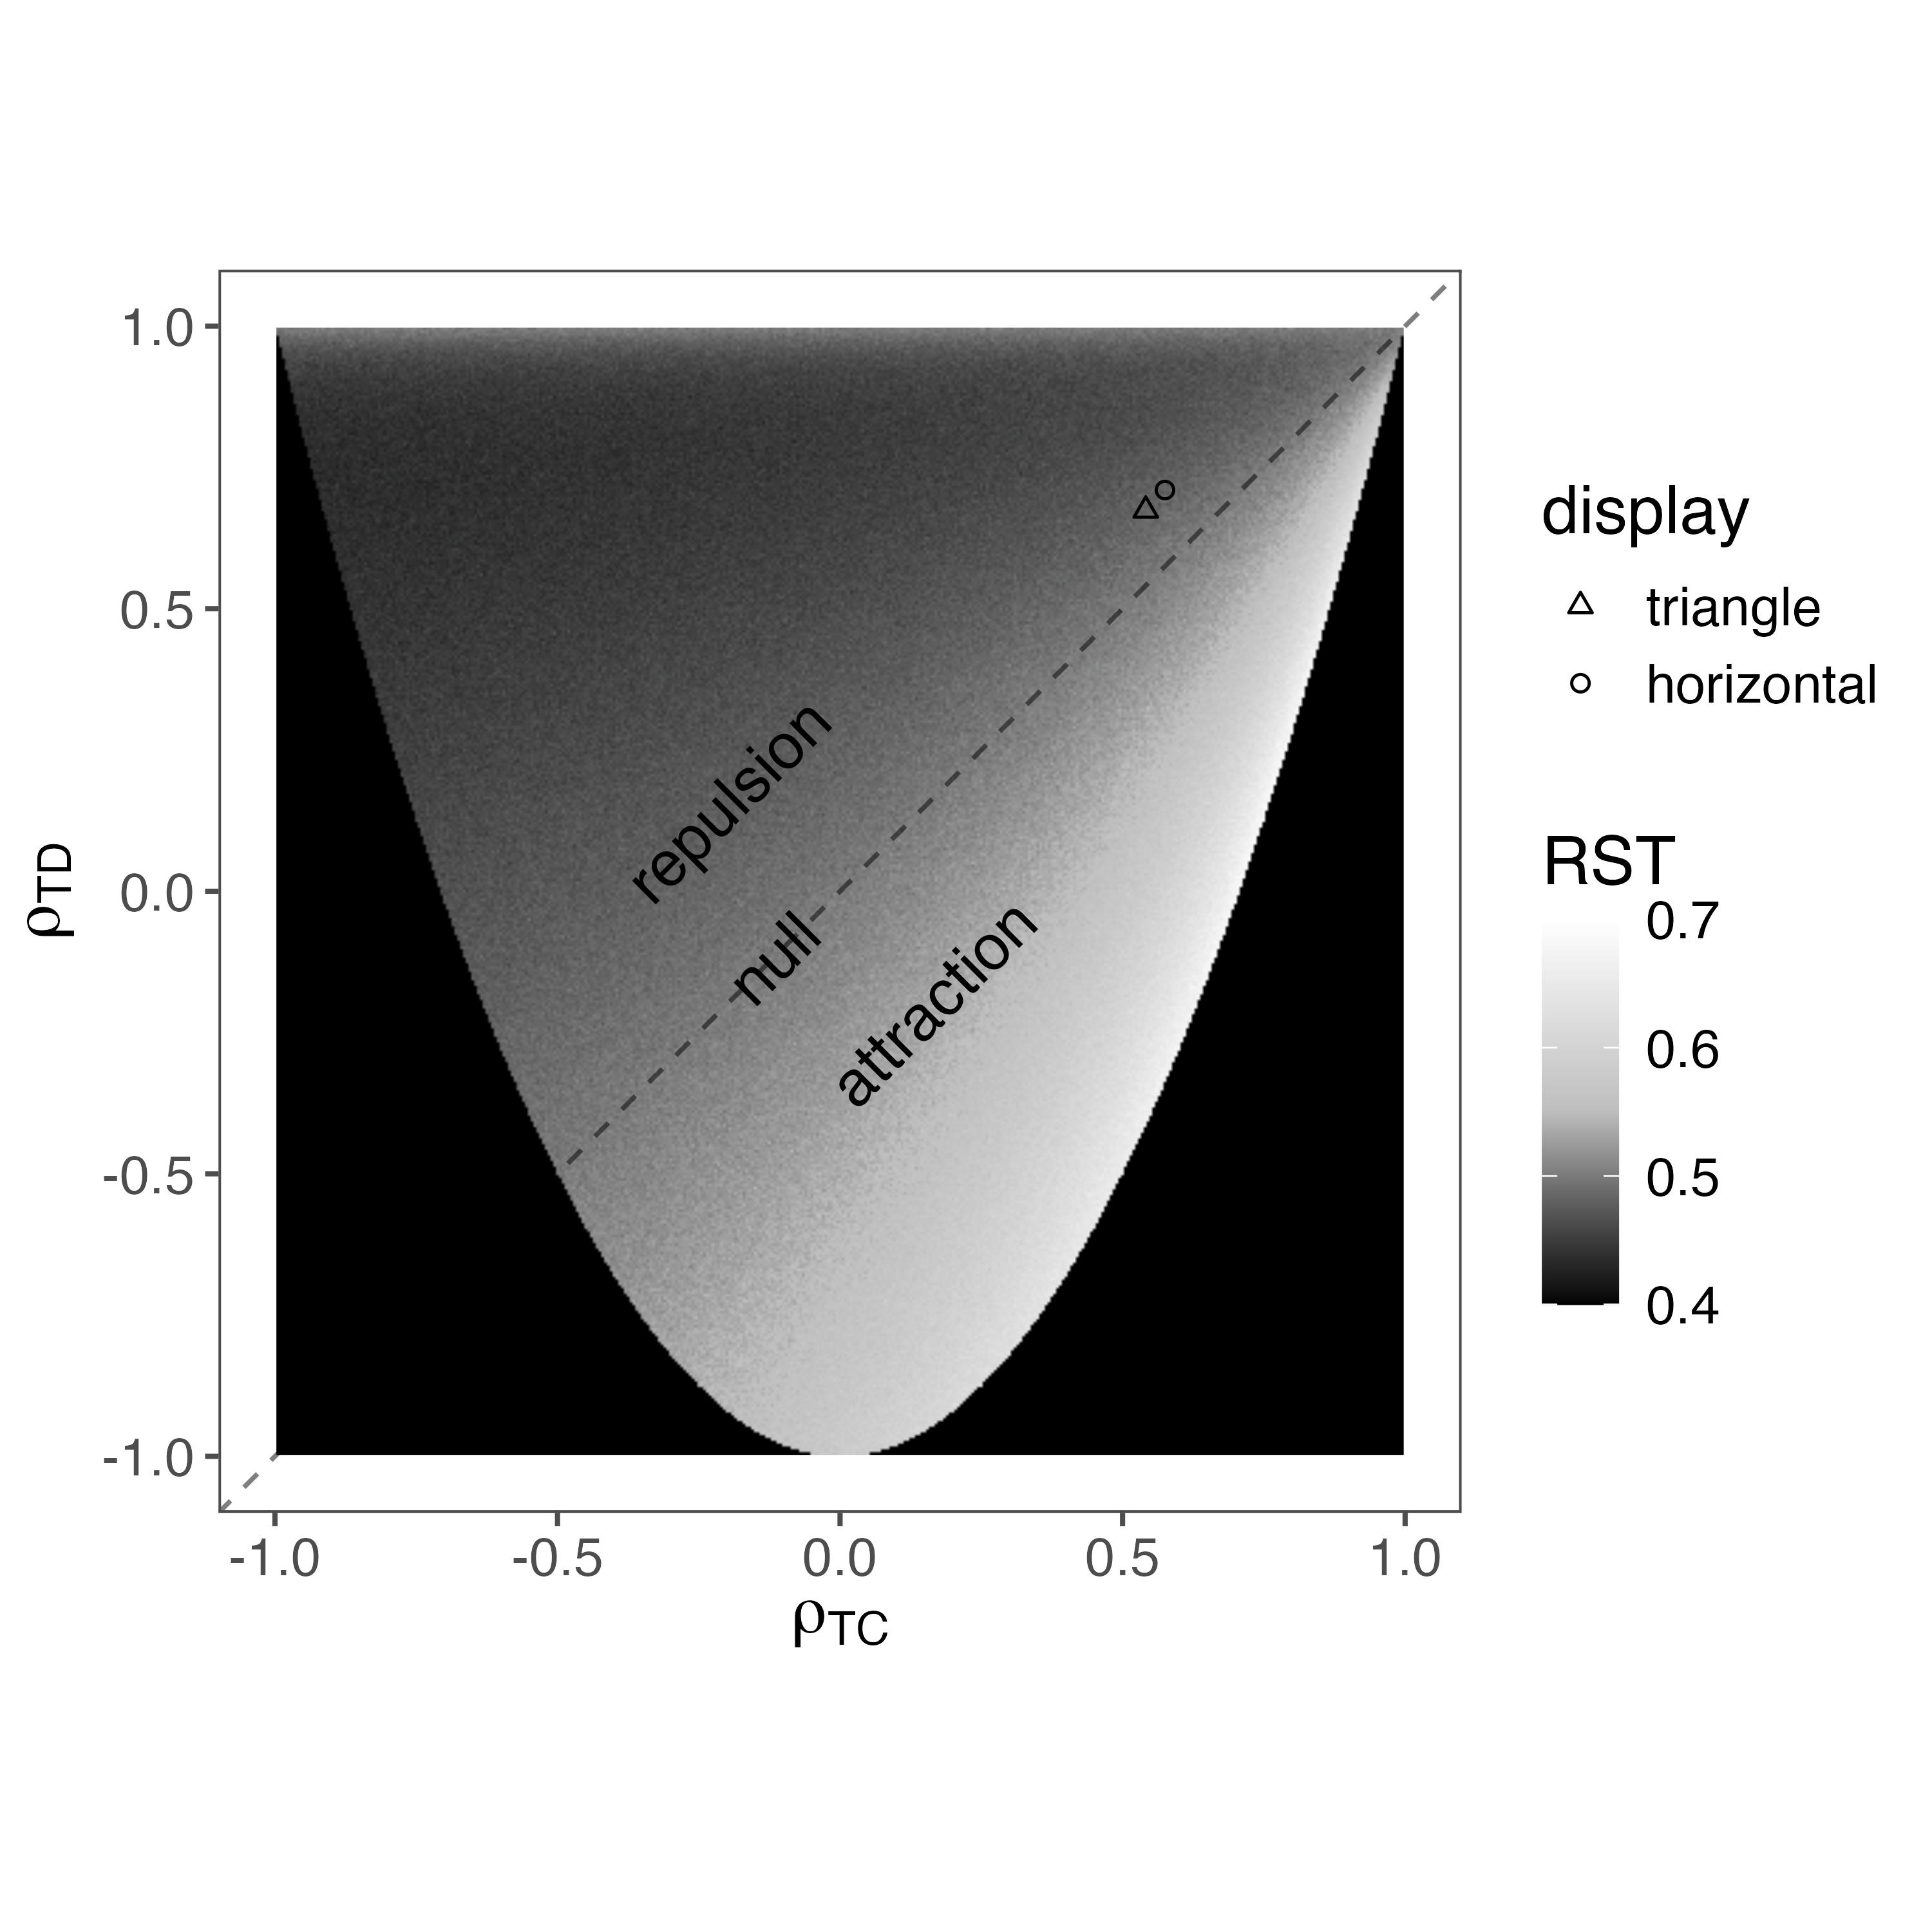
\includegraphics[width=\linewidth]{figures/3d_sim_rst.jpg}
   \caption{Model simulations for the attraction and repulsion effects based on the variation of $\rho_{TD}$ and $\rho_{TC}$. "Regions" of the plot are labeled based on their qualitative predictions for attraction, null, and repulsion effects. The black region is the area where, due to extreme correlations, a positive semi-definite variance-covariance matrix could not be formed and predictions are unavailable. The triangle and circle mark the observed mean correlations from the Experiment 2 triangle and horizontal conditions respectively.}
   \label{fig:3d_model}
\end{figure}

\subsection{Perceptual Correlations as Mechanism for the Repulsion Effect}
I propose that these perceptual correlations may be driving the repulsion effect in \textcite{spektorWhenGoodLooks2018b}'s data. The decoy option is smaller than the the target and competitor options and is thus not always discriminated. The triangle configuration makes discriminability particularly difficult for participants (as I show below in Experiment 1). Simultaneously, however, the fact that target and decoy share an orientation (i.e., both wide or both tall) makes the comparison of these two options easier. When TDD is low, the ease of target-decoy comparison will increase the likelihood that the decoy is perceived to be larger than the target. In statistical terms, the perception of the decoy is more strongly correlated with the perception of the target than with perception of the competitor. These correlations are measured with the $\rho_{TD}$ and $\rho_{CD}$ parameters of the model. According to this account, if $\rho_{TD}>\rho_{CD}$, the perceived areas of target and decoy "move" together and the decoy is more likely to exceed the target than the competitor in ternary choice, particularly if perceptual discriminability is low. The repulsion effect may be driven by perception rather than decision processes. 

In Experiment 1, I first present results from a two-alternative forced-choice experiment to show that these stimuli are easily confusable and that the triangle display of \textcite{spektorWhenGoodLooks2018b} decreases discriminability relative to the horizontal display. I also show that, consistent with the predictions of a perceptual model where $\rho_{TD}>\rho_{TC}=\rho_{CD}$, target-decoy discriminability is in fact greater than competitor-decoy discriminability in binary choice and that target-decoy discriminability increases with TDD. 

In Experiment 2, I combined a psychophysics task with a choice task to estimate the parameters of the perceptual model. In the first phase of the experiment, participants estimate the size of target, decoy, and competitor rectangles on each trial. In the second phase of the experiment, I conducted a standard choice experiment, replicating \textcite{spektorWhenGoodLooks2018b}'s results. I use the data from the first phase of Experiment 2 to obtain stable estimates of  $\boldsymbol{\mu}$ and $\boldsymbol{\Sigma}$ in the perceptual model. Finally, I show that the model, conditioned on the observed parameter estimates, naturally predicts a repulsion effect but not an attraction effect.  

\section{Experiment 1}

The goal of Experiment 1 was to test participants' ability to discriminate between rectangles in the perceptual choice tasks of \textcite{trueblood2013not} and \textcite{spektorWhenGoodLooks2018b}. 
On each trial, participants saw three options (target, competitor, and decoy). After a short delay, two of the rectangles were highlighted and participants chose which of the two rectangles was larger. 
This experiment also included a within-subjects manipulation to compare discriminability in both the triangle display of \textcite{spektorWhenGoodLooks2018b}, Experiment 3, and the horizontal display of \textcite{spektorWhenGoodLooks2018b}, Experiment 4a\footnote{see also \textcite{trueblood2013not}, Experiment 1.}. Otherwise, with a few exceptions discussed below, I follow the stimulus construction and experimental design of \textcite{spektorWhenGoodLooks2018b}, Experiment 3. 

\subsection{Methods}

\subsubsection{Participants.}
Data collection took place at the University of Massachusetts Amherst. 86 undergraduate students participated in exchange for course credit. 1 participant who achieved less than $80\%$ accuracy on catch trials (see below) was excluded from all analyses. Trials with response times (RTs) $<100\text{ms}$ or  $>10000\text{ms}$ were also excluded from all analyses.

\subsubsection{Stimuli.}
The experiment had two types of trials: critical trials and catch trials. 
On each critical trial, the target and competitor had the same area\footnote{Here I simplify \textcite{spektorWhenGoodLooks2018b}'s design by ensuring both focal stimuli had the same area.} but differed on orientation, with one stimulus being wide and the other tall. The decoy always had the same orientation as the target. The height and width of the decoy were reduced proportionally so that the decoy area was always $0\%$, $2\%$, $5\%$, $9\%$, or $14\%$ of the target areas. Because the target and competitor always had the same area, this means that the decoy was also $0\%$, $2\%$, $5\%$, $9\%$, or $14\%$ of the competitor area. These are the TDD values from \textcite{spektorWhenGoodLooks2018b}, plus a $0\%$ level which acted as a baseline\footnote{When TDD=$0\%$, the target and decoy are identical, so labeling is arbitrary.}.

\subsubsection{Design.}
There were 5 blocks of trials. In each block there were 60 critical trials, 12 at each TDD level, and 30 catch trials. Of the 12 critical trials at each TDD level, 6 were presented in a triangle and 6 were presented horizontally. Finally, 3 of the 6 targets in each display condition at each TDD level were wide and 3 were tall. Of each of these 3, one was a target-decoy comparison, one was a target-competitor comparison, and one was a target-competitor comparison. Trial order and rectangle order within each trial were randomized.

On each catch trial, there was one large rectangle and two much smaller rectangles. The large rectangle was $260 \pm U(-40, 40) \text{x} 200 \pm U(-40, 40)$ pixels, with a random orientation. The smaller rectangles were $180 \pm U(-40, 40) \text{x} 120 \pm U(-40, 40)$ pixels, one wide and one tall.

On every trial, the rectangles were displayed in either a triangle or horizontal display (see Figure~\ref{fig:spektor_stim}). The horizontal distance between all rectangles was constant, but 25 pixels of jitter was added to each rectangle's vertical location.

Stimuli were presented on computer monitors with a resolution of 1920 x 1080 pixels. The experiment was programmed with jsPsych \parencite{deleeuwJsPsychJavaScriptLibrary2015}. 

\subsubsection{Procedure.}
On each trial, participants saw three rectangles, labeled 1, 2, and 3 (from left to right). The rectangles appeared for 1825ms total, but after 500ms, two of the rectangles changed to a darker shade. After all three rectangles disappeared from the screen, participants were asked to select which of the two darker rectangles had the larger area.

\subsection{Results}

\subsubsection{Catch Trials.}
Participants performed well on the catch trials. The mean percentage correct in the triangle display was $92.6\% (SD=3.77)$, and the mean percentage correct in the triangle display was $93.2\% (SD=3.52)$. 

\subsubsection{Critical Trials.}
I first checked the baseline TDD level data (TDD=$0\%$) across to make sure that participants were indifferent between pairs of options when they had identical area. The mean percentage of target choices in target-competitor trials was $48.99\%$ (SD=10.18). The mean percentage of competitor choices in competitor-decoy trials was $49.80\%$ (SD=11.30). The mean percentage of target choices in target-decoy trials was $49.47\%$ (SD=12.06). Participants were indifferent between all pairs of options in the $\text{TDD}=0\%$ trials, so I do not consider these trials further.

The primary analysis was performed on the target-decoy and competitor-decoy trials, excluding the TDD=$0\%$ trials. In these trials participants' task is simply to not select the decoy option on a given trial. I present mean choice proportions across conditions in Figure~\ref{fig:e1_data}. Participants' performance indeed improves with TDD. Furthermore, their performance is better when stimuli are displayed in the horizontal configuration than in the triangle configuration, and it is also better in target-decoy trials compared to competitor-decoy trials. Finally, there is an interaction, such that as TDD increases, the target-decoy performance is even better than the competitor-decoy performance. See the Appendix for inferential statistics which support these conclusions.

\begin{figure}
   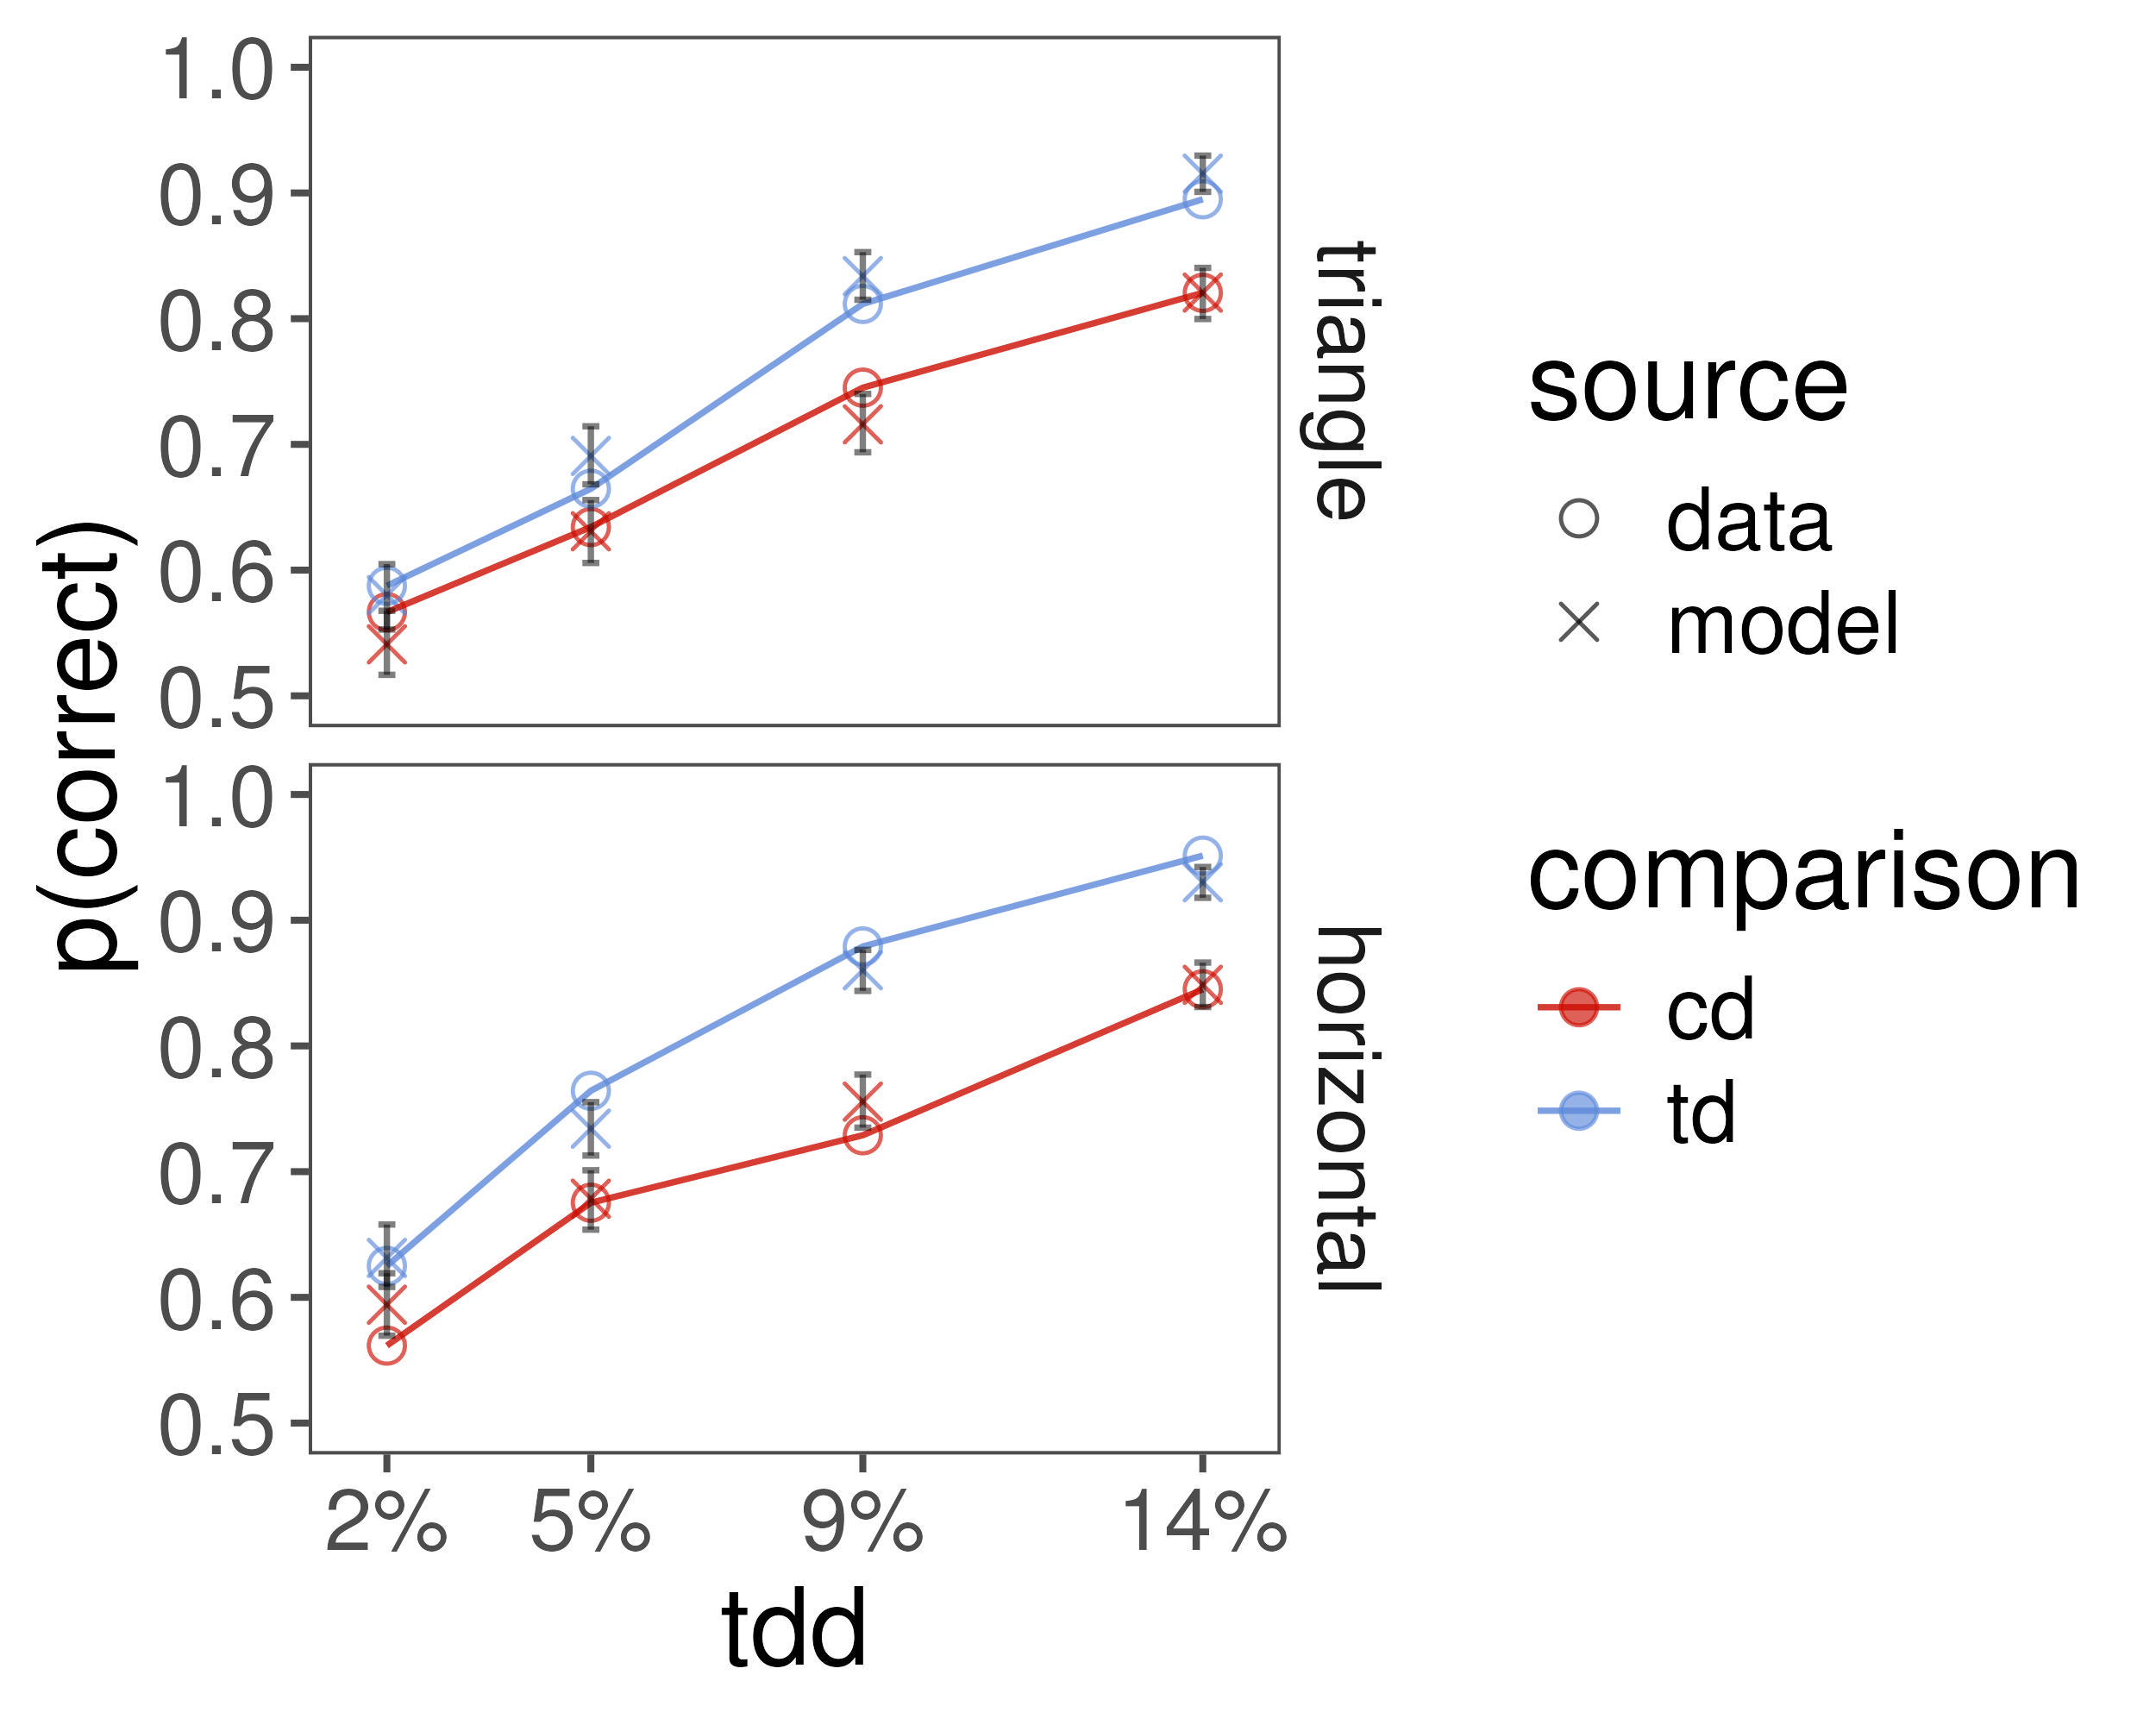
\includegraphics[width=\textwidth]{figures/m14_model_preds_v_data.jpeg}
   \caption{Experiment 1, mean choice proportions by stimulus display, TDD, and comparison. td=target-decoy trials, dc=competitor-decoy trials. Model predictions come from the Bayesian hierarchical logistic regression presented in the Appendix. Error bars are $95\%$ HDIs on the mean.}
   \label{fig:e1_data}
\end{figure}

\subsubsection{Discussion}
In Experiment 1, I showed that participants are not always able to discriminate between target-decoy and competitor-decoy stimuli. I also show that this discriminability increases with TDD and that overall discriminability is better in the horizontal compared to the triangle display. Finally, through the interaction of comparison-pair and TDD, I show that target-decoy discriminability increases with TDD at a higher rate than competitor-decoy discriminability. 

\section{Experiment 2}
I continue this line of research in Experiment 2, where I used a psychophysics task to estimate the mean perceived area and correlations between perceived area to the target, competitor, and decoy rectangles. Experiment 2 used the \textit{method of cross-modal matching} \parencite{stevensCrossmodalityMatchingBrightness1965}, where participants adjusted the size of a circle to match the perceived area for each rectangle. On each trial, participants saw three rectangles and three circles, each labeled 1, 2, and 3. Participants adjusted the size of the circle corresponding to each rectangle, until they believed the two to have equal area. I also replicate \textcite{spektorWhenGoodLooks2018b}'s choice data in a second phase of the experiment. Finally, I used a between-subjects manipulation to display the rectangle stimuli in either the horizontal or triangle displays of \textcite{spektorWhenGoodLooks2018b}.

\subsection{Methods}
\subsubsection{Participants.}
Data collection took place at the University of Massachusetts Amherst. 521 undergraduate students participated in exchange for course credit. 68 participants did not complete the full experiment within the 1 hour time limit and were removed from all analyses. 

\subsubsection{Stimuli.}
In the circle adjustment phase there were three types of trials: critical trials, filler trials, and catch trials. On each critical trial, the target and competitor had the same area but differed on orientation, with one stimulus being wide and the other tall. The decoy always had the same orientation as the target. I varied TDD from $2\%$, $5\%$, $9\%$, and $14\%$. I also varied the target, competitor, and decoy stimuli to fall on three diagonals. In pixels, the small and larger focal stimulus dimension values on the lower, middle, and upper diagonals were $[60, 135]$, $[90, 165]$, and $[120,195]$. I reduced the absolute size of the target/competitor stimuli from Experiment 1 to Experiment 2 to accomodate the circle adjustment phase (see procedure below).

On filler trials, I randomly sampled three rectangles by sampling three heights and widths from the distribution $U(56,195)$px, encompassing the full range of stimuli from the critical trials.

On the catch trials, I randomly sampled one rectangle from the lower diagonal and two from the upper diagonal. This ensured that one stimulus was always larger than the other two and allowed me to remove inattentive participants.

The choice phase had identical trial types with the exception that there were no catch trials, only critical and filler trials.

\subsubsection{Design.}
Across both phases, I varied display condition between-subjects and TDD, diagonal, target-decoy orientation within-subjects. After removing participants (see above), there were 223 participants in the horizontal display condition and 230 participants in the triangle display condition. 

In the circle adjustment phase, there were 4 blocks, each with 40 trials. Each block consisted of 24 critical trials, 14 filler trials, and 2 catch trials. Within the critical trials, there were 6 trials at each level of TDD. In 3 of these 6 trials the target and decoy were oriented wide (choice set $[w,h,d_{w}]$), and in the other 3 target and decoy were oriented tall (choice set $[w,h,d_{h}]$). 

In the choice phase, there were 4 blocks, each with 34 trials. 24 of these trials were critical trials and 10 were filler trials. Of these 24 critical trials, there were 6 trials at each level of TDD. Within each 6, there were 3 trials where target and decoy were oriented wide and 3 were target and decoy were oriented tall. 

\subsubsection{Procedure.}

The experiment took place in two phases: 

On each circle adjustment trial, three gray rectangles appeared in the lower left corner of the screen, either in a triangle or horizontal display. In the upper right, three gray circles appeared in the upper right of the screen, in the same display as the rectangles (see Figure~\ref{fig:circle_exp_display} ). A small amount of jitter ($U(-15,15)\text{px}$) was added to the position of each rectangle and the corresponding circle. Each circle started with an area of 78 square pixels (i.e., with a radius of 5), the minimum size I allowed in the experiment. Participants used the mouse to adjust the circle. Within a single trial, they were free to adjust the circles in any order they liked or to go re-adjust a circle as much as they liked. There was no time limit to each adjustment trial. The maximum circle area allowed was 65144 square pixels\footnote{I arrive at this number based on the maximum area the circles could be while only appearing on the right half of the screen and maintaining the same horizontal distance from each other as the corresponding rectangles.}. When a participant finished adjusting the circles on a trial, they clicked the "Submit" button located on the lower right hand corner of the screen. 

The circle adjustment phase began with three practice trials, followed by the 4 blocks of experimental trials. At the beginning of each experimental block, participants completed 3 calibration trials. Calibration trials were identical to filler trials, with the caveat that I provided feedback after participants' responses. After participants submitted their responses on a trial, a red circle appeared around each adjusted circle, showing the true area of the corresponding rectangle. 

Throughout the circle phase, I kept track of the deviations between the true rectangle areas and the participants' adjusted circle areas. At the end of each block, I computed the current mean deviation, and, depending on this value, told the participant that they were either over or under-adjusting, on average.

The choice phase began with 3 practice trials. Participants were not provided feedback during these practice trials. 

On each choice trial, three rectangles appeared in the center of the screen in a horizontal or triangle display. There was no vertical jitter added here. Participants were told to select the rectangle with the largest area by clicking on it.

At the end of the choice phase, I let each participant know their percentage correct from the choice phase. Note that in a critical trial, a correct response is simply one where they did not select the decoy, as the target and competitor rectangles always had the same area.

Stimuli were presented on computer monitors with a resolution of 1920 x 1080 pixels. The experiment was programmed with GNU Octave \parencite{octave} and PsychoPhysics Toolbox \parencite{brainardPsychophysicsToolbox1997}. 

\begin{figure}
   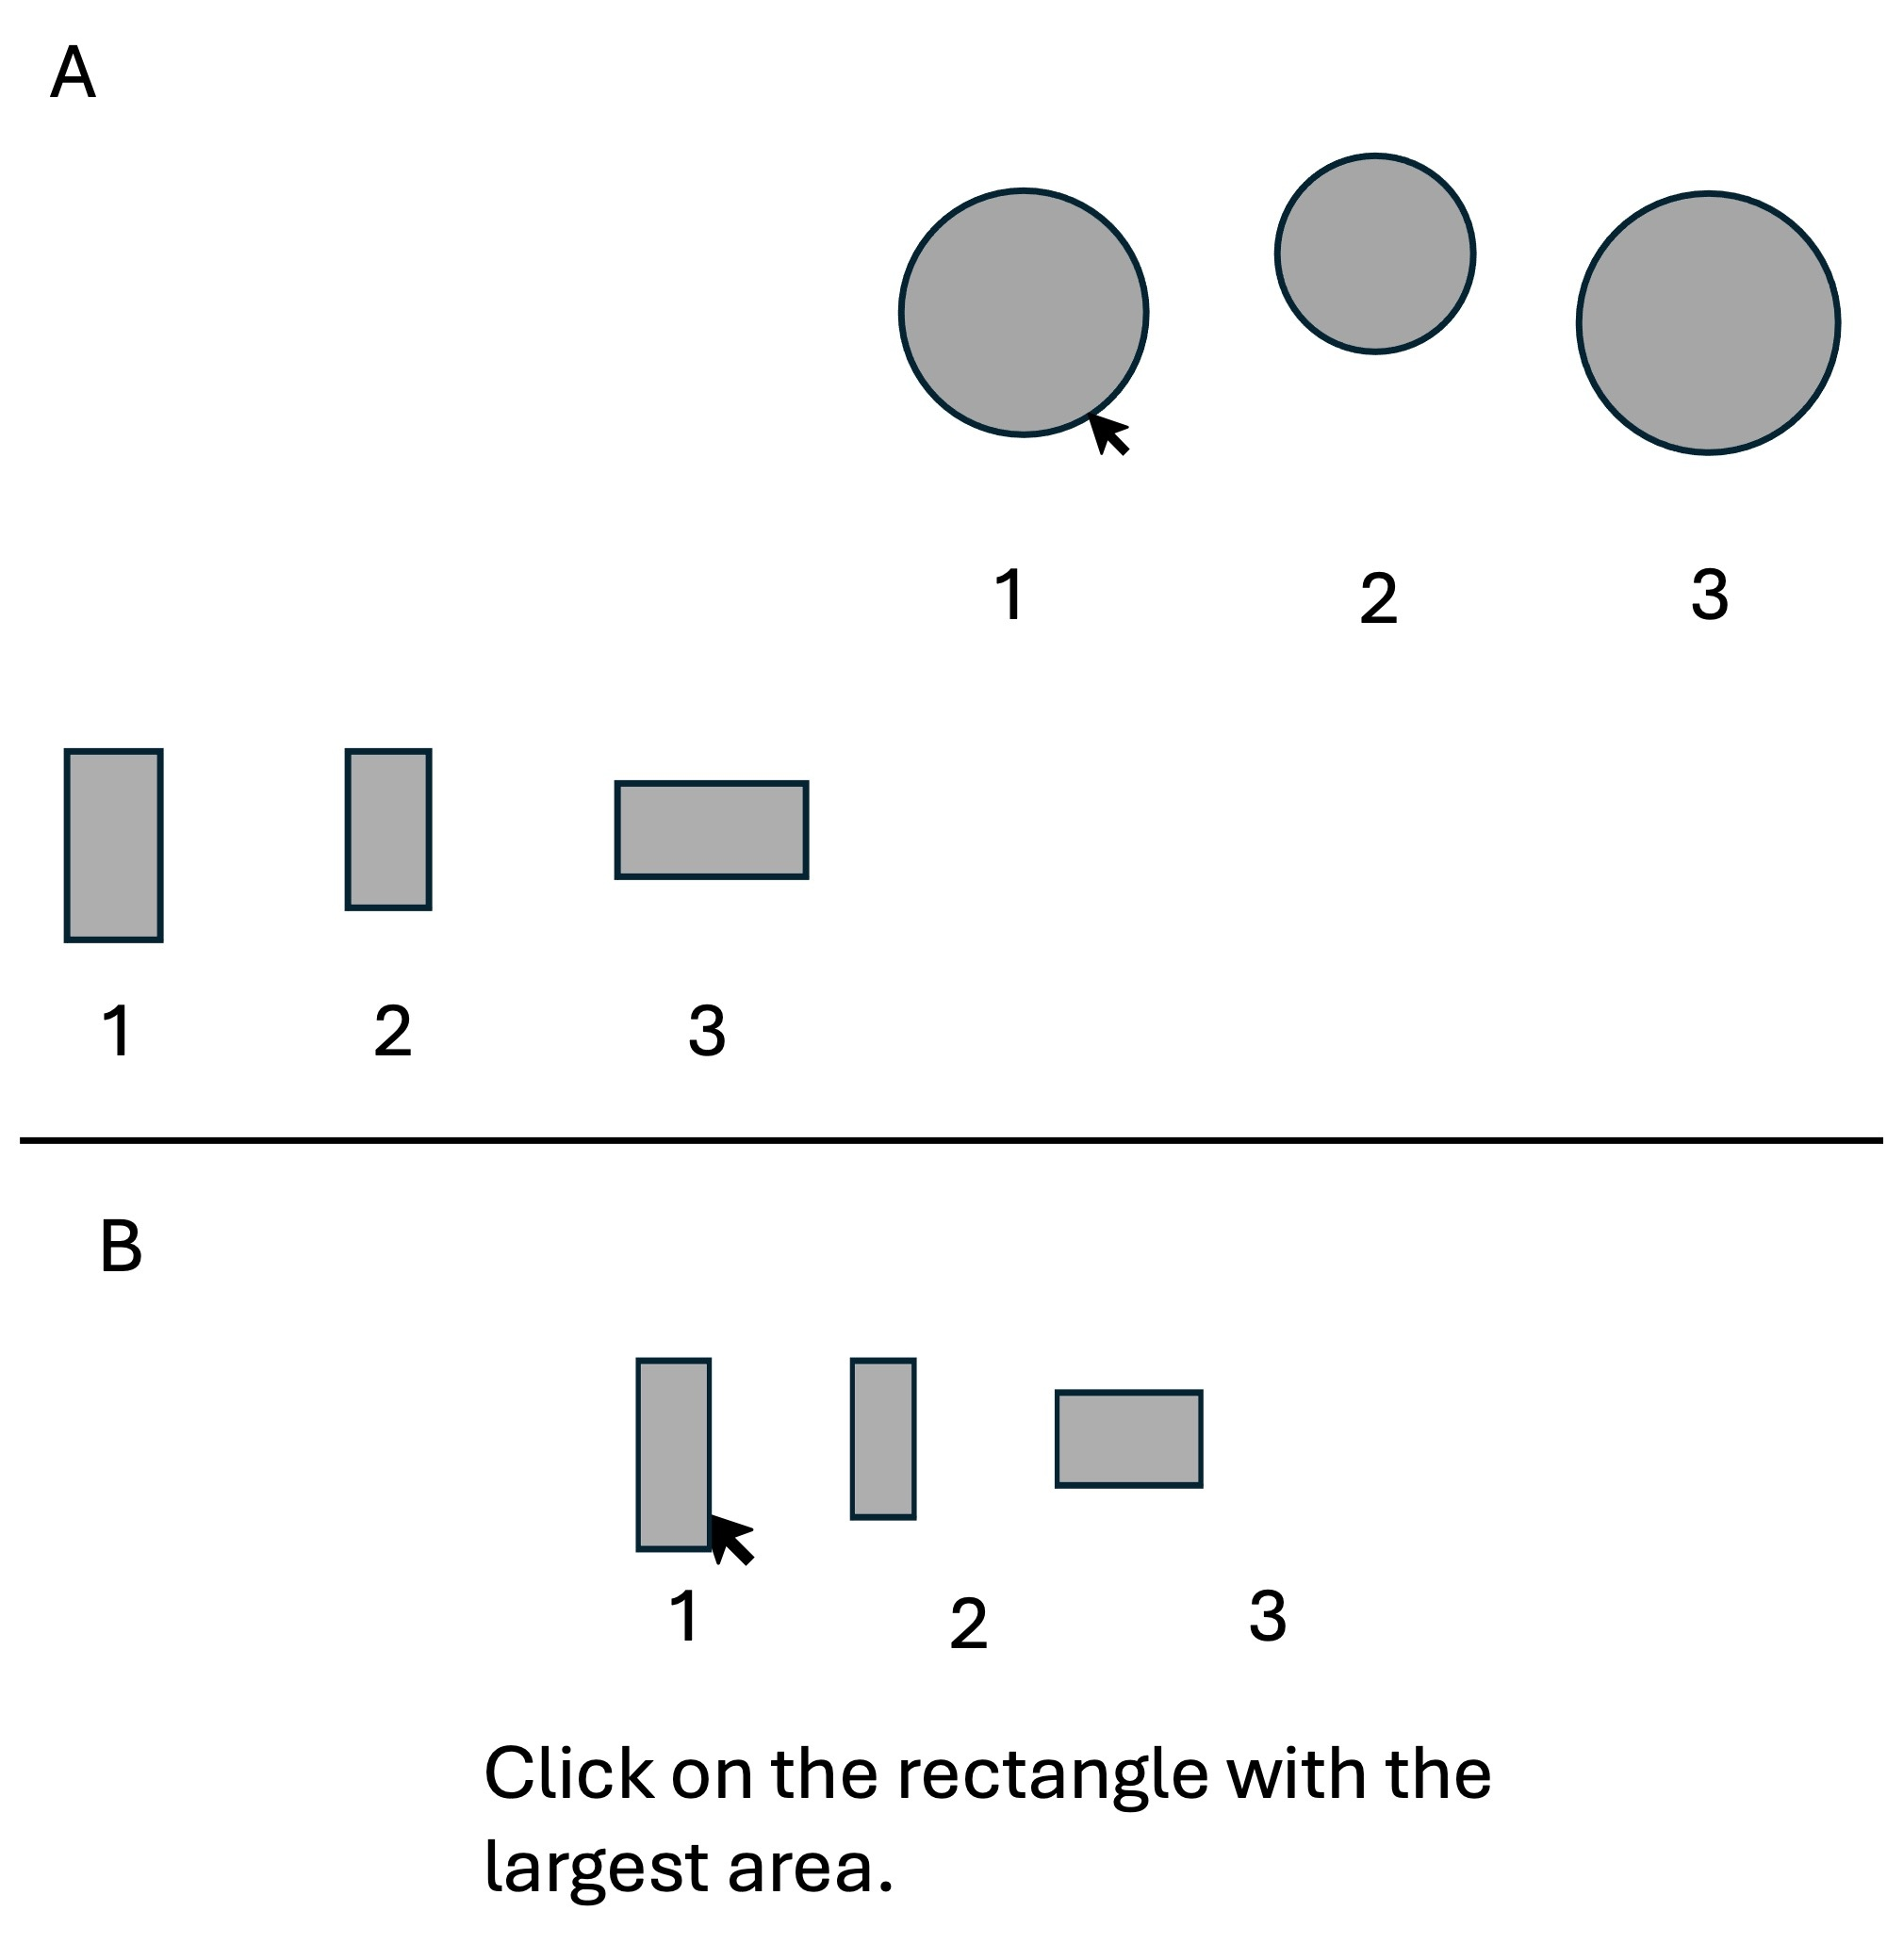
\includegraphics[width=\linewidth]{figures/circle_exp_display.jpg}
   \caption{Example trials from Experiment 2. A: Circle adjustment phase. B: Choice phase. This an example of trials in the horizontal display condition.}
   \label{fig:circle_exp_display}
\end{figure}

\subsection{Results}
\subsubsection{Data Processing}
Given the difficulty of the circle adjustment task, the data required processing to ensure that outlier trials and participants did not influence our estimates of $\mathbf{Omega}$.

First, I removed all participants who did not give correct responses on $75\%$ ($6/8)$ of the catch trials. A correct response entails estimating the larger rectangle to be the largest on the trial. 10 participants were removed from all analyses after they failed to achieve at least $75\%$ correct on catch trials (see below for details). This left a total of 443 participants.

Next, from the remaining participants, I first natural log-transformed all responses. I then dropped all trials where at least one circle was not adjusted (i.e., at least one circle was left at the starting size).

I then removed outlier participants using the following procedure:

I fit a linear regression to each individual participants' data, regressing each log circle area on each corresponding log rectangle area. I then computed an $R^2$ for each participant. I then removed all participants whose $R^2$ fell below the $5\%$ quantile for all $R^2$s, which in this case was $.3975$. This removed 23 subjects, leaving us with a total of 420 participants, 213 in the triangle display condition and 207 in the horizontal display condition. Of the remaining participants, $R^2$ values were high ($M=.67,SD=.12$), indicating they could generally perform the task.

From the $420$ partipants whose data I analyzed, I removed outlier trials from the critical trial data. I did so to ensure that any outliers do not influence our estimates of $\rho_{TD}$, $\rho_{TC}$, or $\rho_{CD}$. I z-transformed all log circle areas within each participant and diagonal. I remove all critical trials where at least one z-score had an absolute value above $3.5$. This led to $102$ trials being dropped. I dropped $0$, $1$, $2$, and $4$ critical trials from $339$, $62$, $18$, and $1$ participants, respectively. 

After all circle phase data processing, I were left with $20371$ trials in the triangle display condition and $19809$ trials in the horizontal display condition. 

For the choice phase, I only retained participants whose data I retained in the circle phase.

\subsubsection{Circle Phase Results - Critical Trials}
Before modeling our data, I wanted to ensure that participants could successfully perform the task. While I do not expect perfect performance in an absolute sense, I do require adequate relative performance. 

To assess performance on the critical trials, I computed the mean difference between actual log area and estimated log area for each subject, stimulus pair (i.e., target-competitor, target-decoy, competitor-decoy), and actual difference. I plot these via a set of boxplots in Figure~\ref{fig:circle_boxplots}. Although participants vary considerably in their judgments, I find that on average, participants' adjusted circle areas increase with the absolute size of rectangles. 


\begin{figure}
   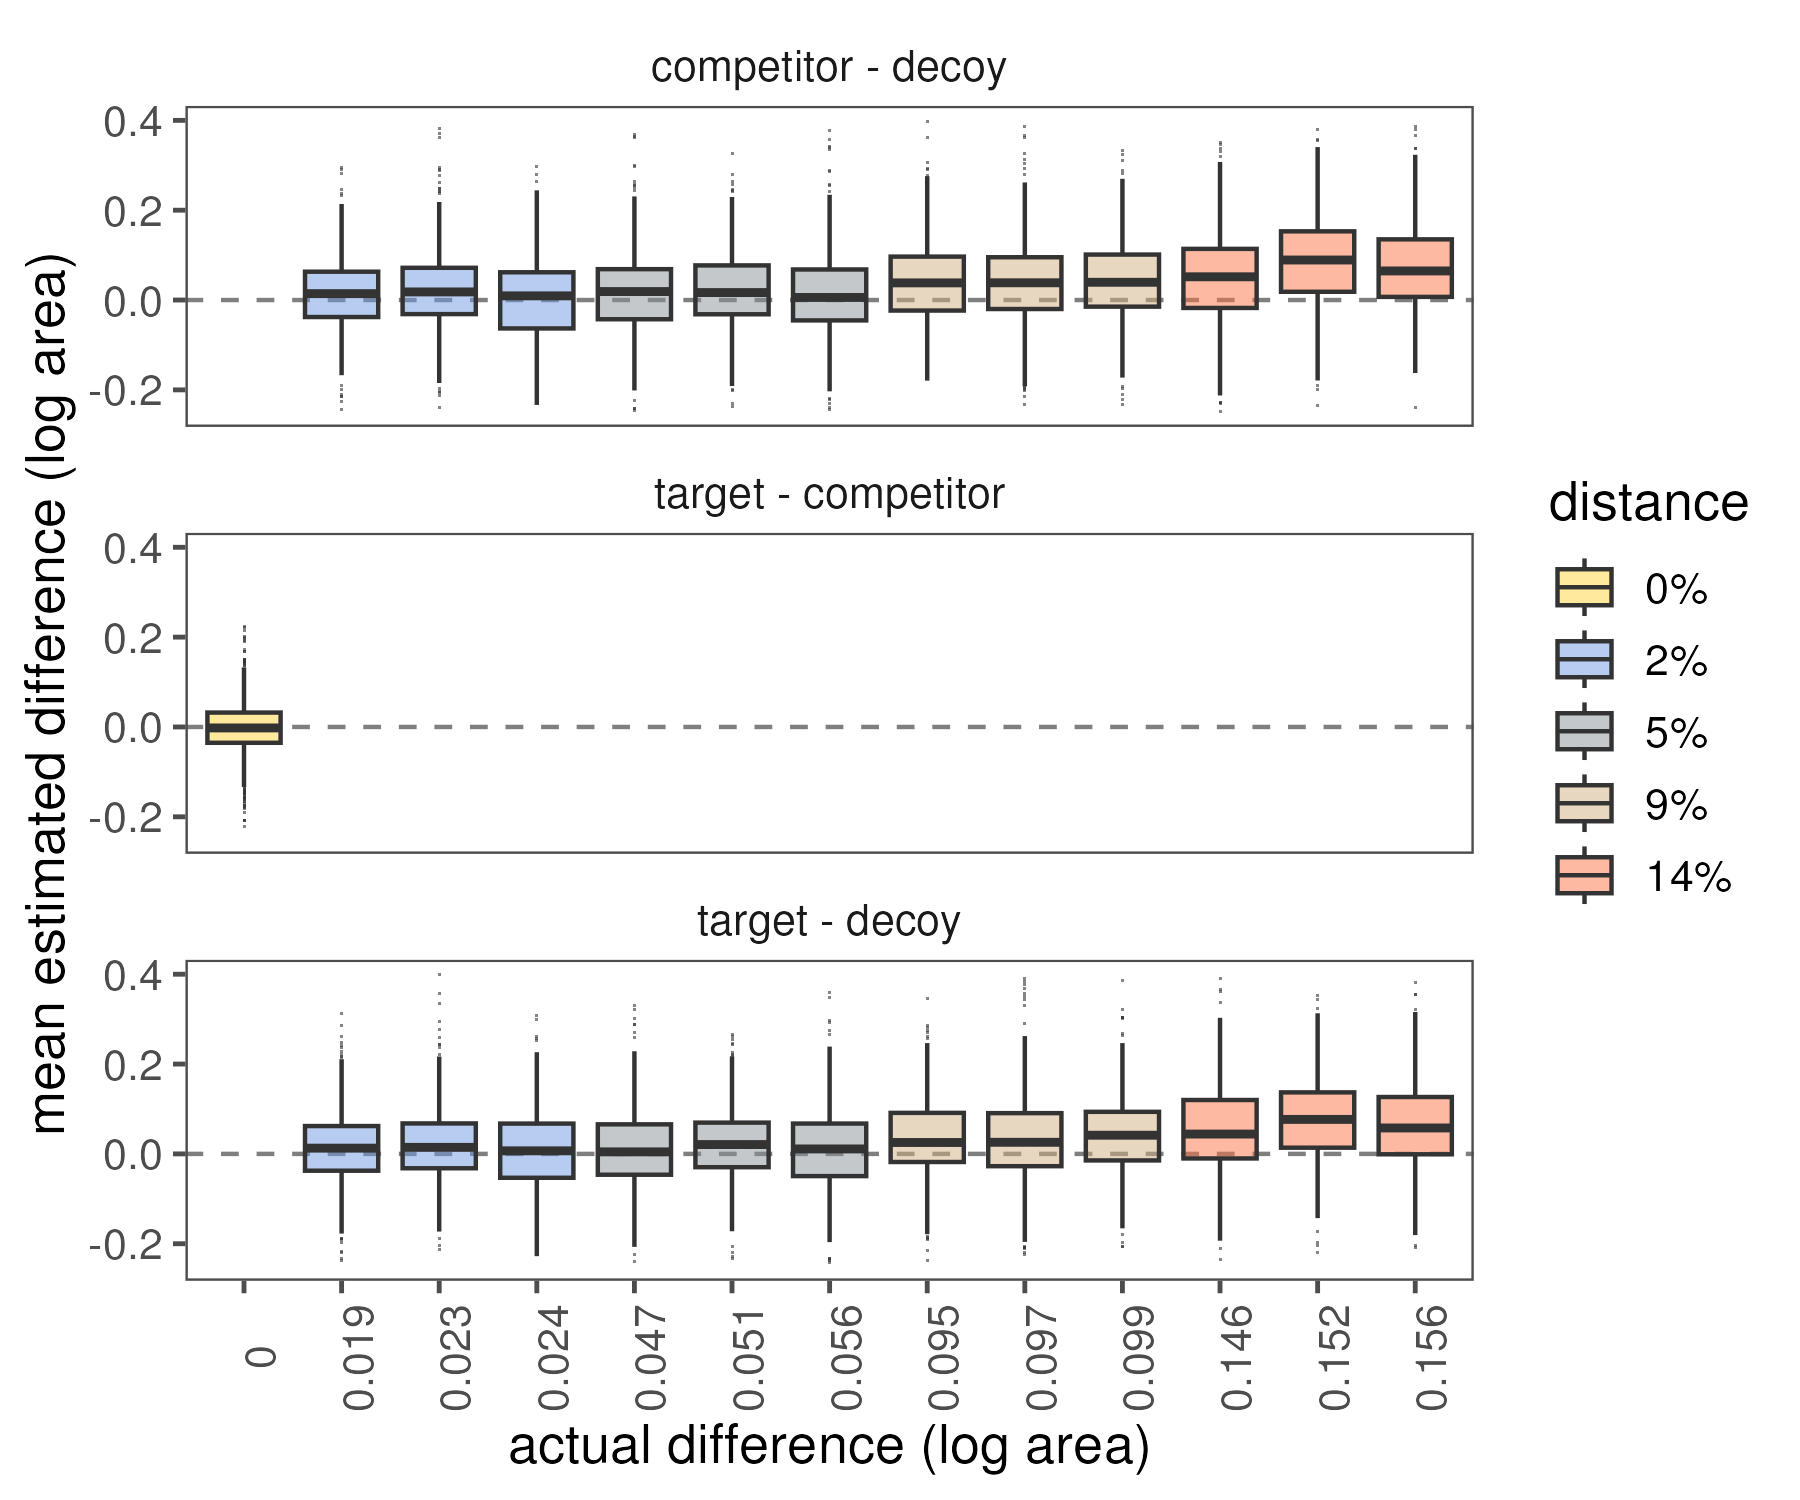
\includegraphics[width=\textwidth]{figures/circleAreaPhase_boxplot_meanlogdiffs_no_outliers.jpeg}
   \caption{Boxplot of subject-level mean error in area estimations, split by stimulus pair, TDD, and absolute discrepancy in rectangle area. Note that because the target and competitor rectangles always had equal areas, the true difference is always 0.}
   \label{fig:circle_boxplots}
\end{figure}

I next present scatterplots of all pairwise circle areas from each trial, see Figure~\ref{fig:raw_cors}. I present these to be transparent about the raw data and to illustrate the necessity of a statistical model to understand these correlations. 

\begin{figure}
   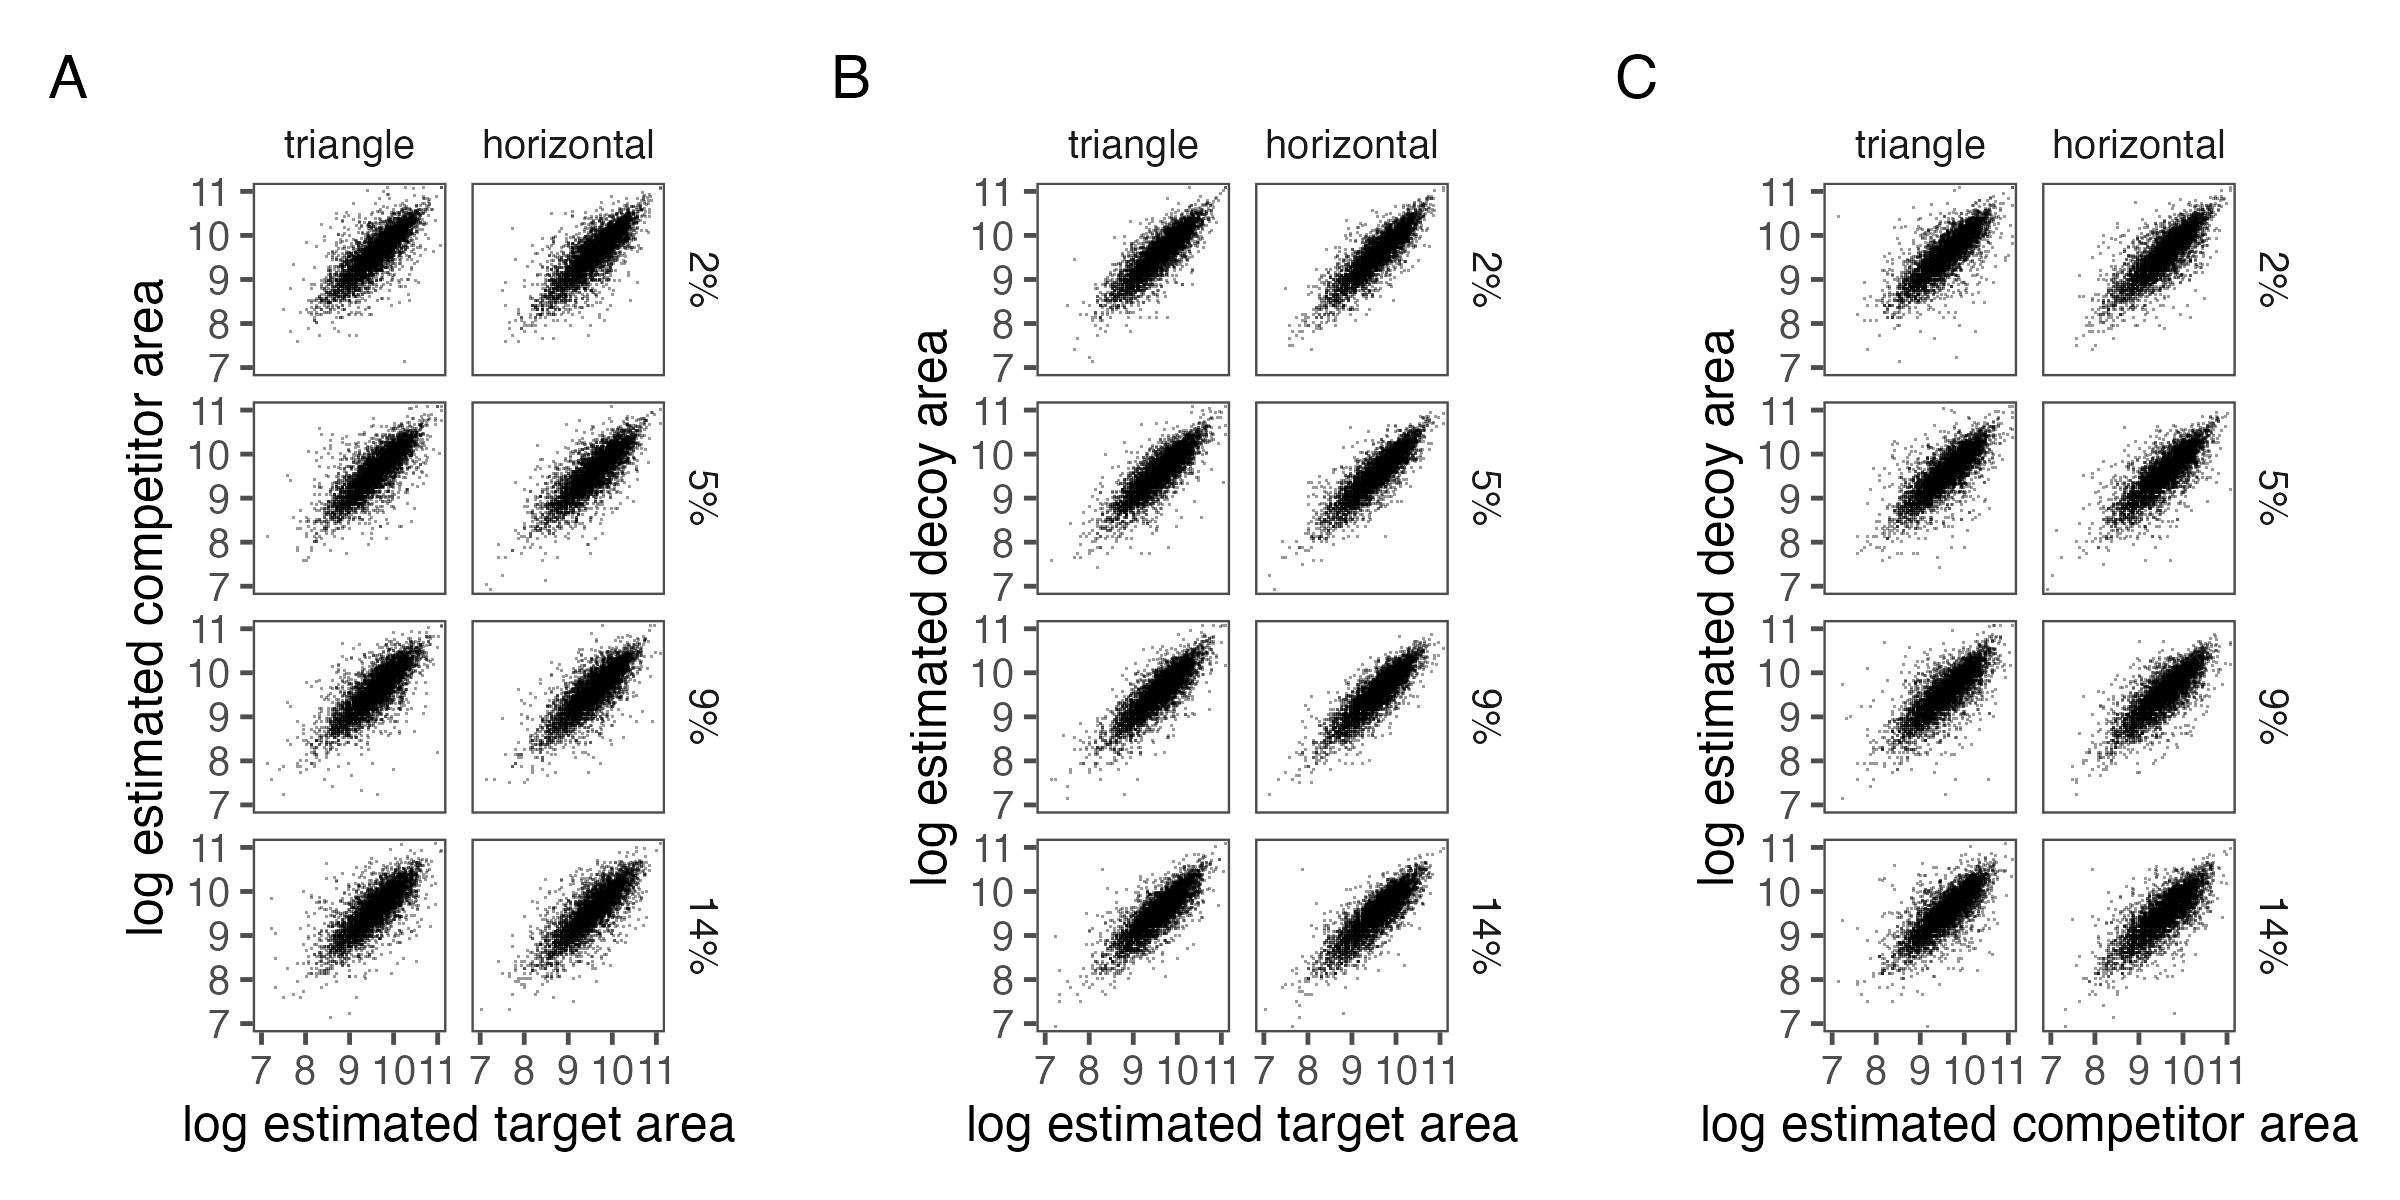
\includegraphics[width=\textwidth]{figures/circleAreaPhase_cor_plot_all_no_outliers.jpg}
   \caption{Scatterplots of target-competitor (A), target-decoy (B), and competitor-decoy (C) correlations, split by display condition and TDD.}
   \label{fig:raw_cors}
\end{figure}

Computing raw correlations, without accounting for subject and trial-level differences, will grossly inflate the size of these correlations. Moreover, any differences between, say, $\rho_{TD}$ and $\rho_{CD}$ are bound to be small. I used Bayesian hierarchical modeling to estimate the parameters of a multivariate normal distribution (as outlined in the introduction), with parameters $\boldsymbol{\mu}$ and $\boldsymbol{\Sigma}$. I present the details of the model in the Appendix but present the main results below.

I assume that, for participant $i$, on each critical trial $j$, the perceived target, competitor, and decoy areas $\mathbf{X}_i$ are sampled from a multivariate normal distribution with mean vector $\boldsymbol{\mu_{ij}}$ and variance-covariance matrix $\boldsymbol{\Sigma}$. 

As discussed in the Introduction, I decompose sigma into the $S\boldsymbol{\Omega}S$, where the diagonal elements of $S$ are population standard deviations and the off diagonal elements are $0$. $\boldsymbol{\Omega}$ is 3 x 3 correlation matrix.  

I focus on the estimates of $\boldsymbol{\mu}$ and $\boldsymbol{\Omega}$ in the main text and discuss the details of the modeling, along with $\S$ estimates, in the Appendix. 

I show mean estimates of $\boldsymbol{\mu}$ in Figure~\ref{fig:e2mu} and show estimates of $\boldsymbol{\Omega}$ in Figure~\ref{fig:omega}. In both conditions, $\rho_{TD}$ is larger than both $\rho_{CD}$ and $\rho_{TC}$, while $\rho_{CD}$ and $\rho_{TC}$ do not differ from each other. 

\begin{figure}
   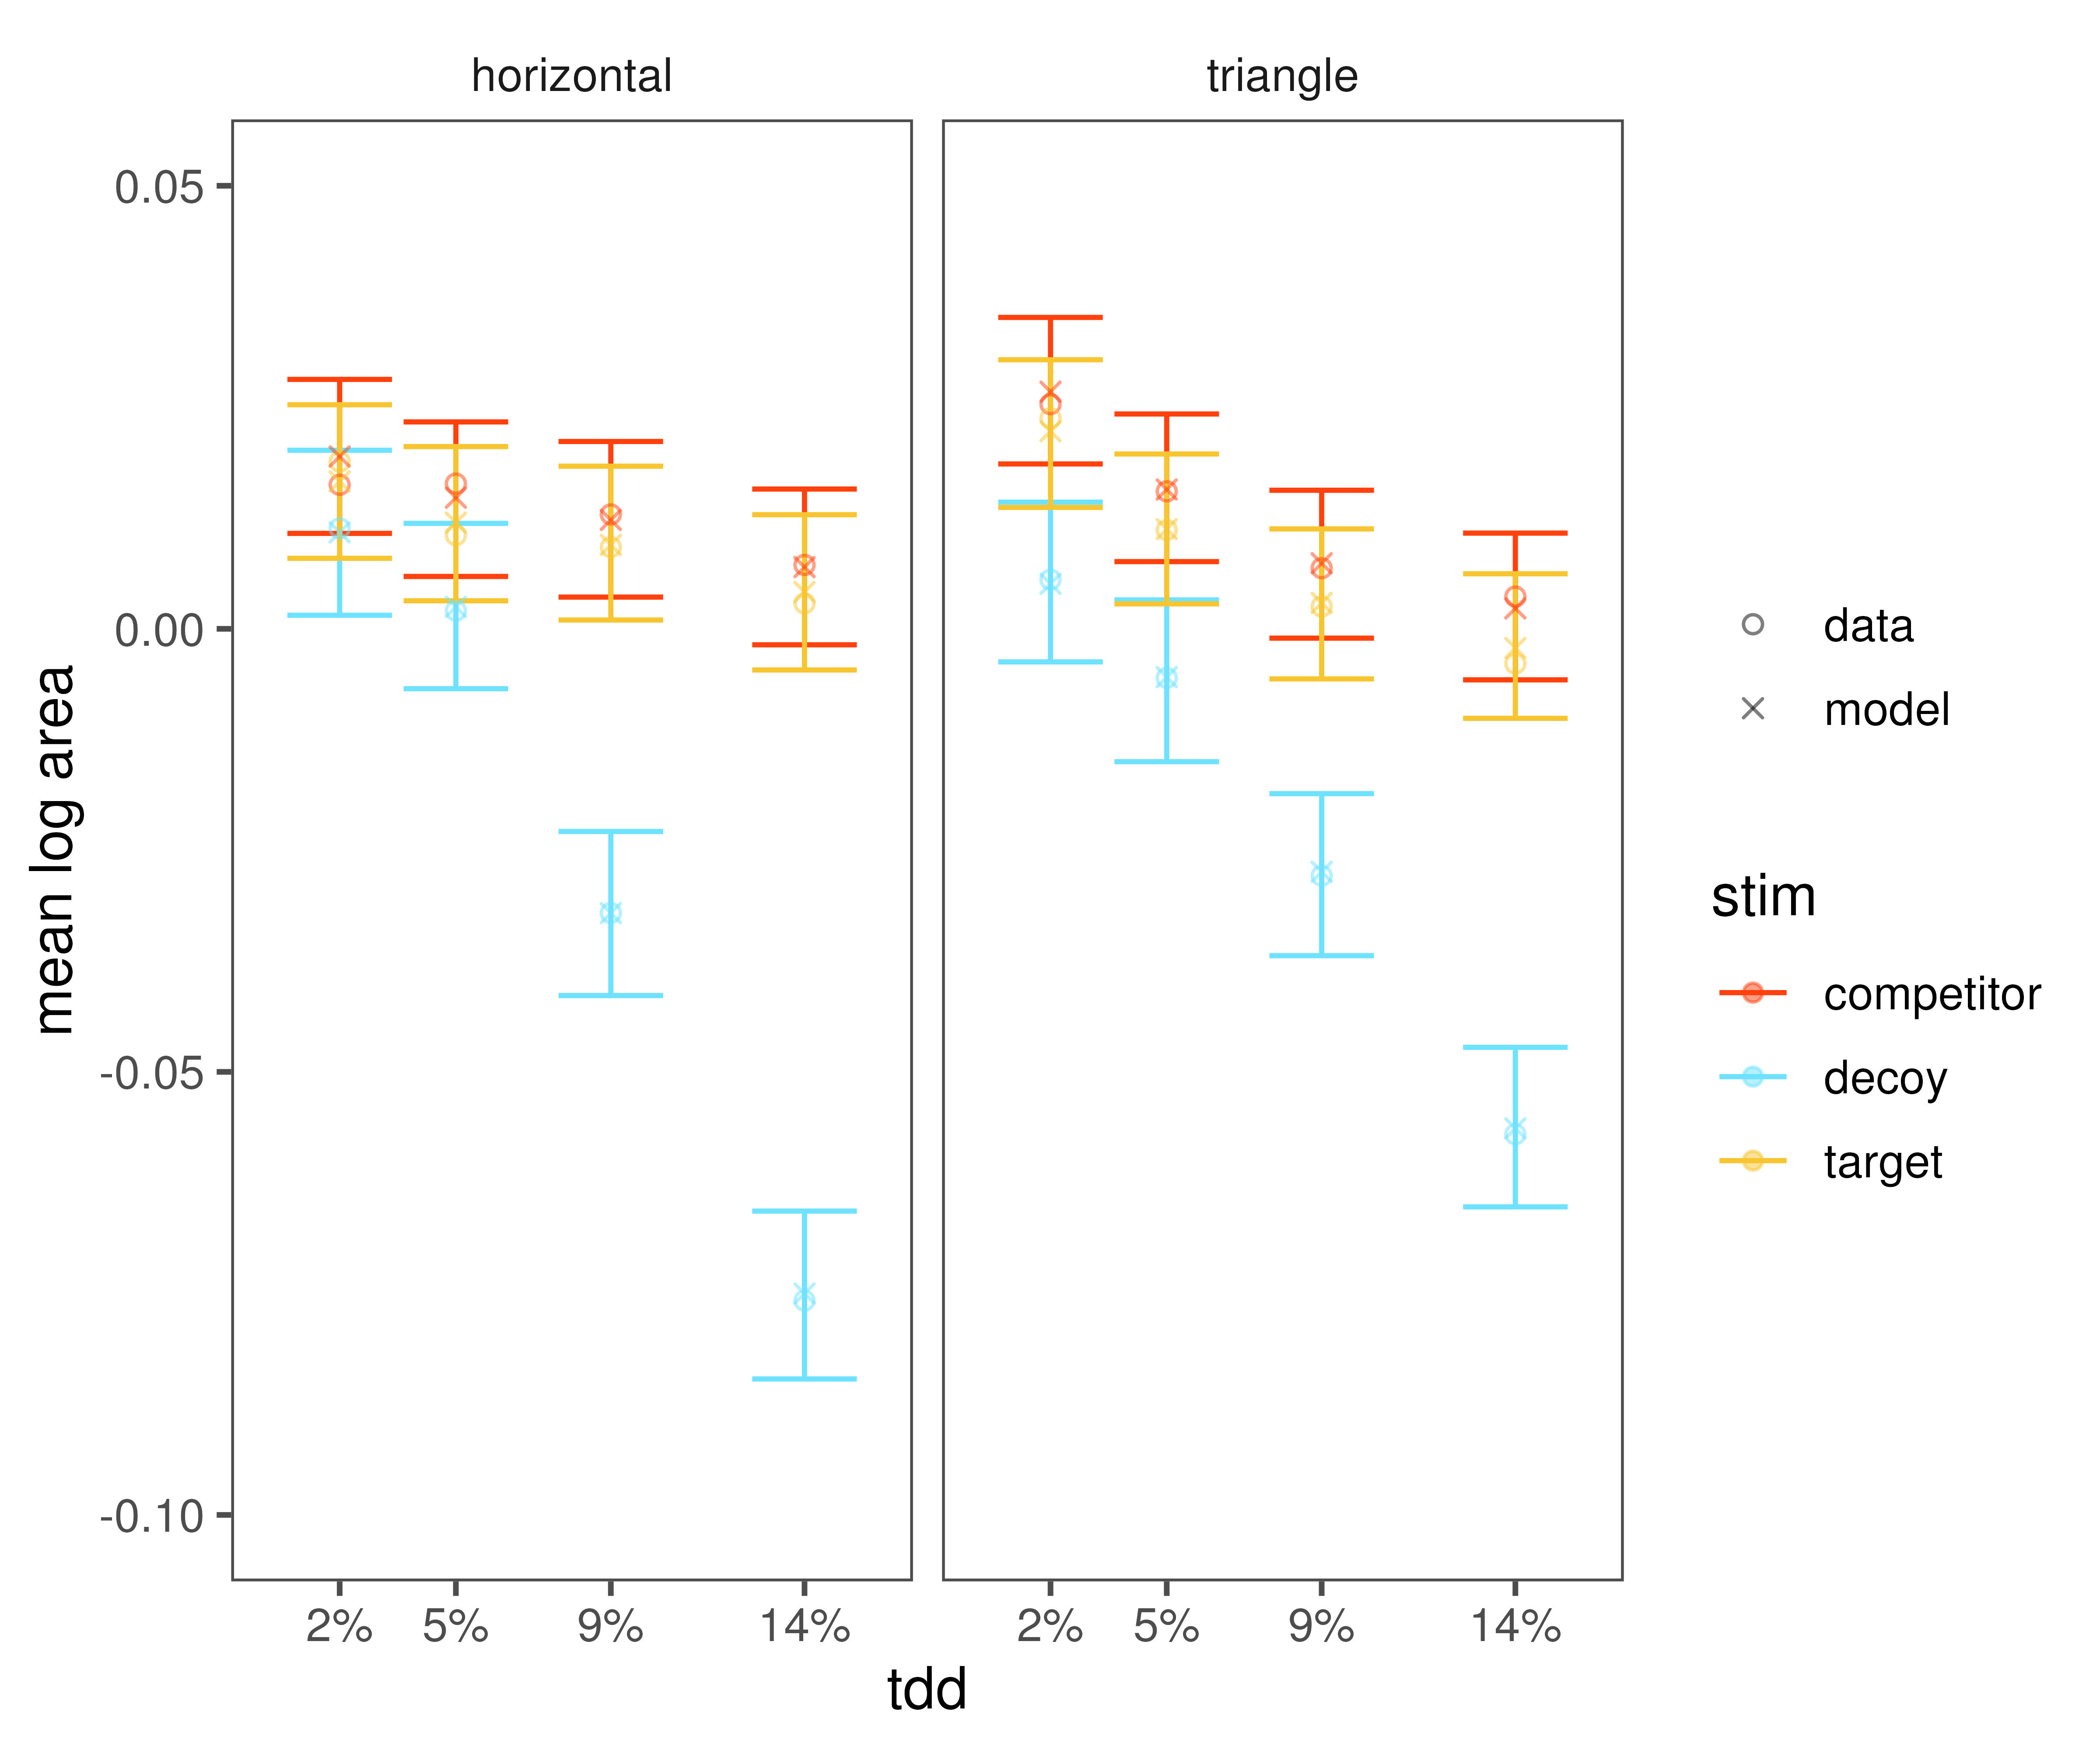
\includegraphics[width=\textwidth]{figures/bayes_circle_area_mu_sigma_constant_comp_effect_model_v_data_collapsed.jpeg}
   \caption{$\boldsymbol{\mu}$ estimates from Experiment 2.}
   \label{fig:e2mu}
\end{figure}

\begin{figure}
   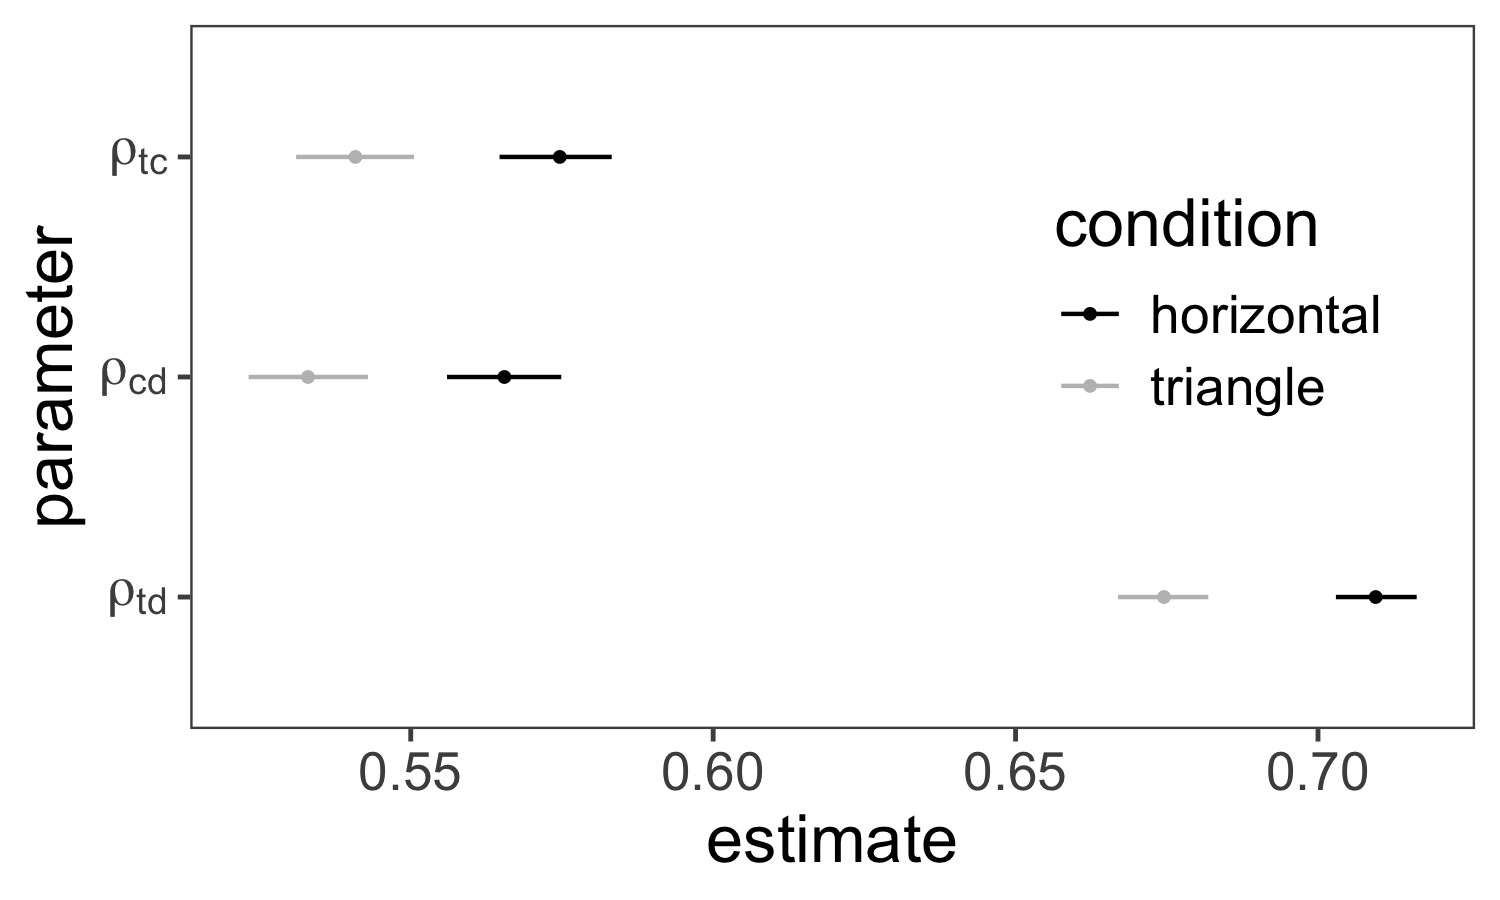
\includegraphics[width=\textwidth]{figures/bayes_circle_area_sigma_constant_comp_effect_omega_plot.jpeg}
   \caption{Posterior estimate of $\boldsymbol{\Omega}$ (off-diagonal parameters) across display conditions. Lines show $95\%$ HDIs.  Dots indicate means.}
   \label{fig:omega}
\end{figure}

\subsubsection{Choice Results}

I present mean choice proportions across display conditions and TDD in Figure~\ref{fig:e2_choiceprops}. I replicate the qualitative results of \textcite{spektorWhenGoodLooks2018b}. At low levels of TDD, I find a repulsion effect in both display conditions. At higher levels of TDD, I either find a null effect (triangle condition) or an attraction effect (horizontal condition). 

To ensure that this result is not an artifact of averaging across choice sets, I present mean changes in choice proportion for the options $w$ and $h$ across the two choice sets $[w,h,d_{w}]$ and $[w,h,d_{h}]$ (see Figure~\ref{fig:e2_choicedeltas}). These results also show that low levels of TDD create a repulsion effect, while higher levels create a null or attraction effect. See the Appendix for inferential statistics that support these conclusions.

\begin{figure}
   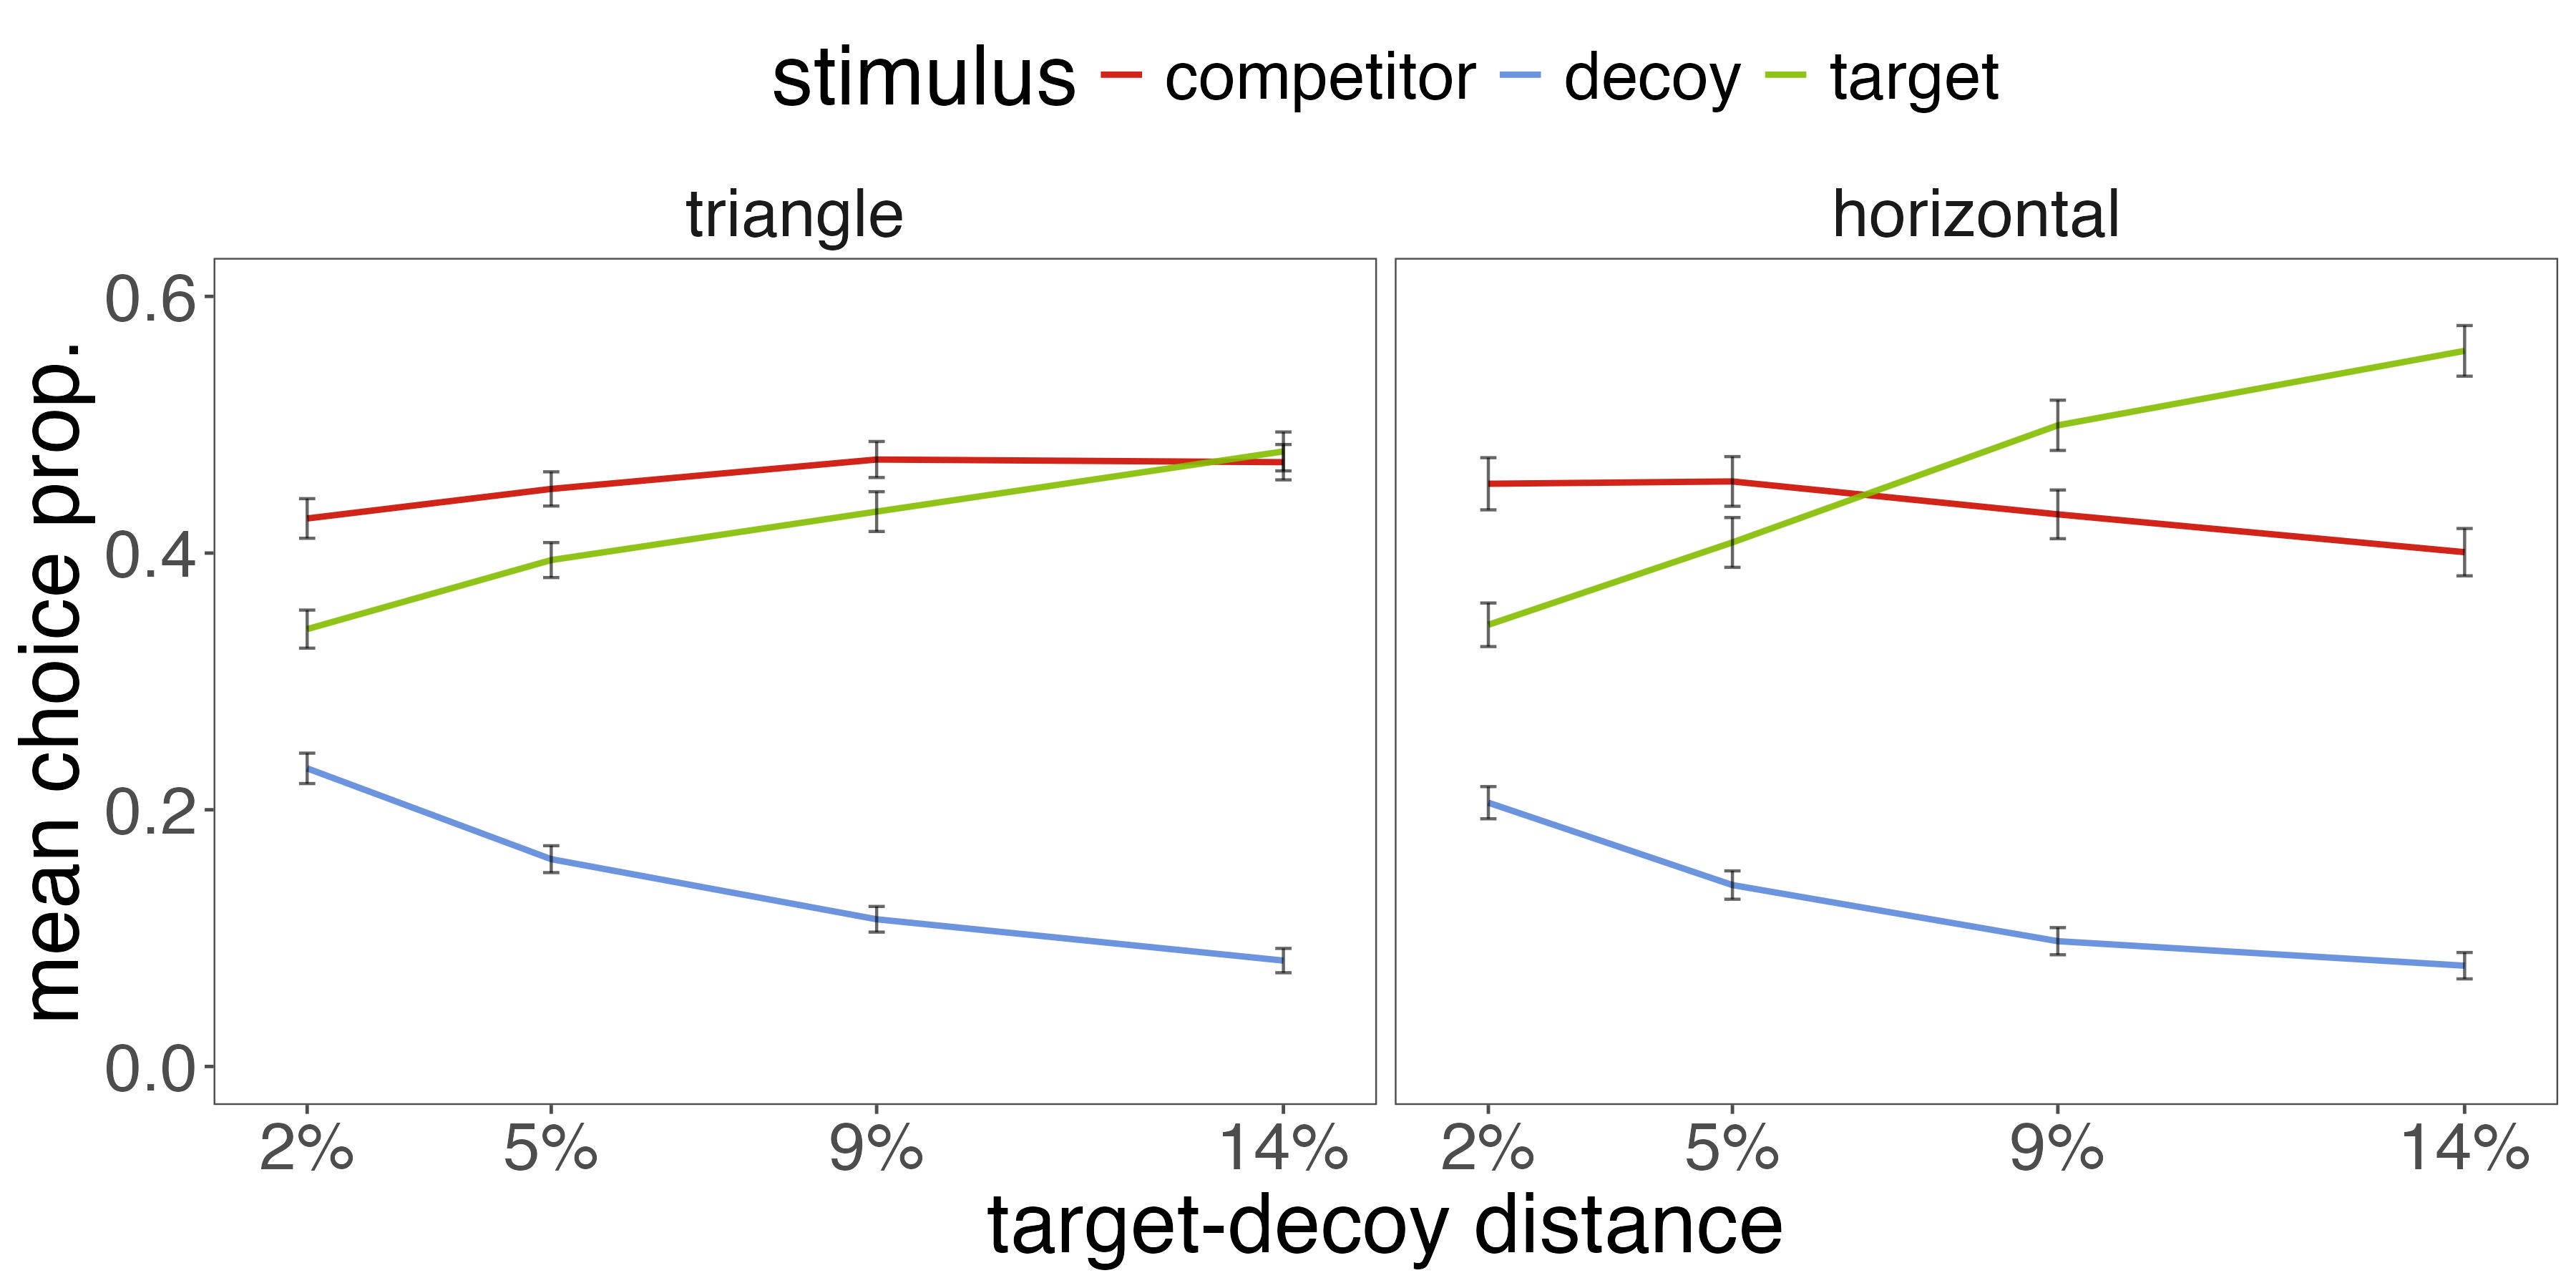
\includegraphics[width=\textwidth]{figures/choicePhase_att_trials_mean_choice_props_collapsed.jpg}
   \caption{Mean choice proportions for target, competitor, and decoy options, by TDD and display condition. THIS FIGURE IS A PLACEHOLDER. WILL CHANGE WITH HDIs FROM STAT. MODEL.}
   \label{fig:e2_choiceprops}
\end{figure}

\begin{figure}
   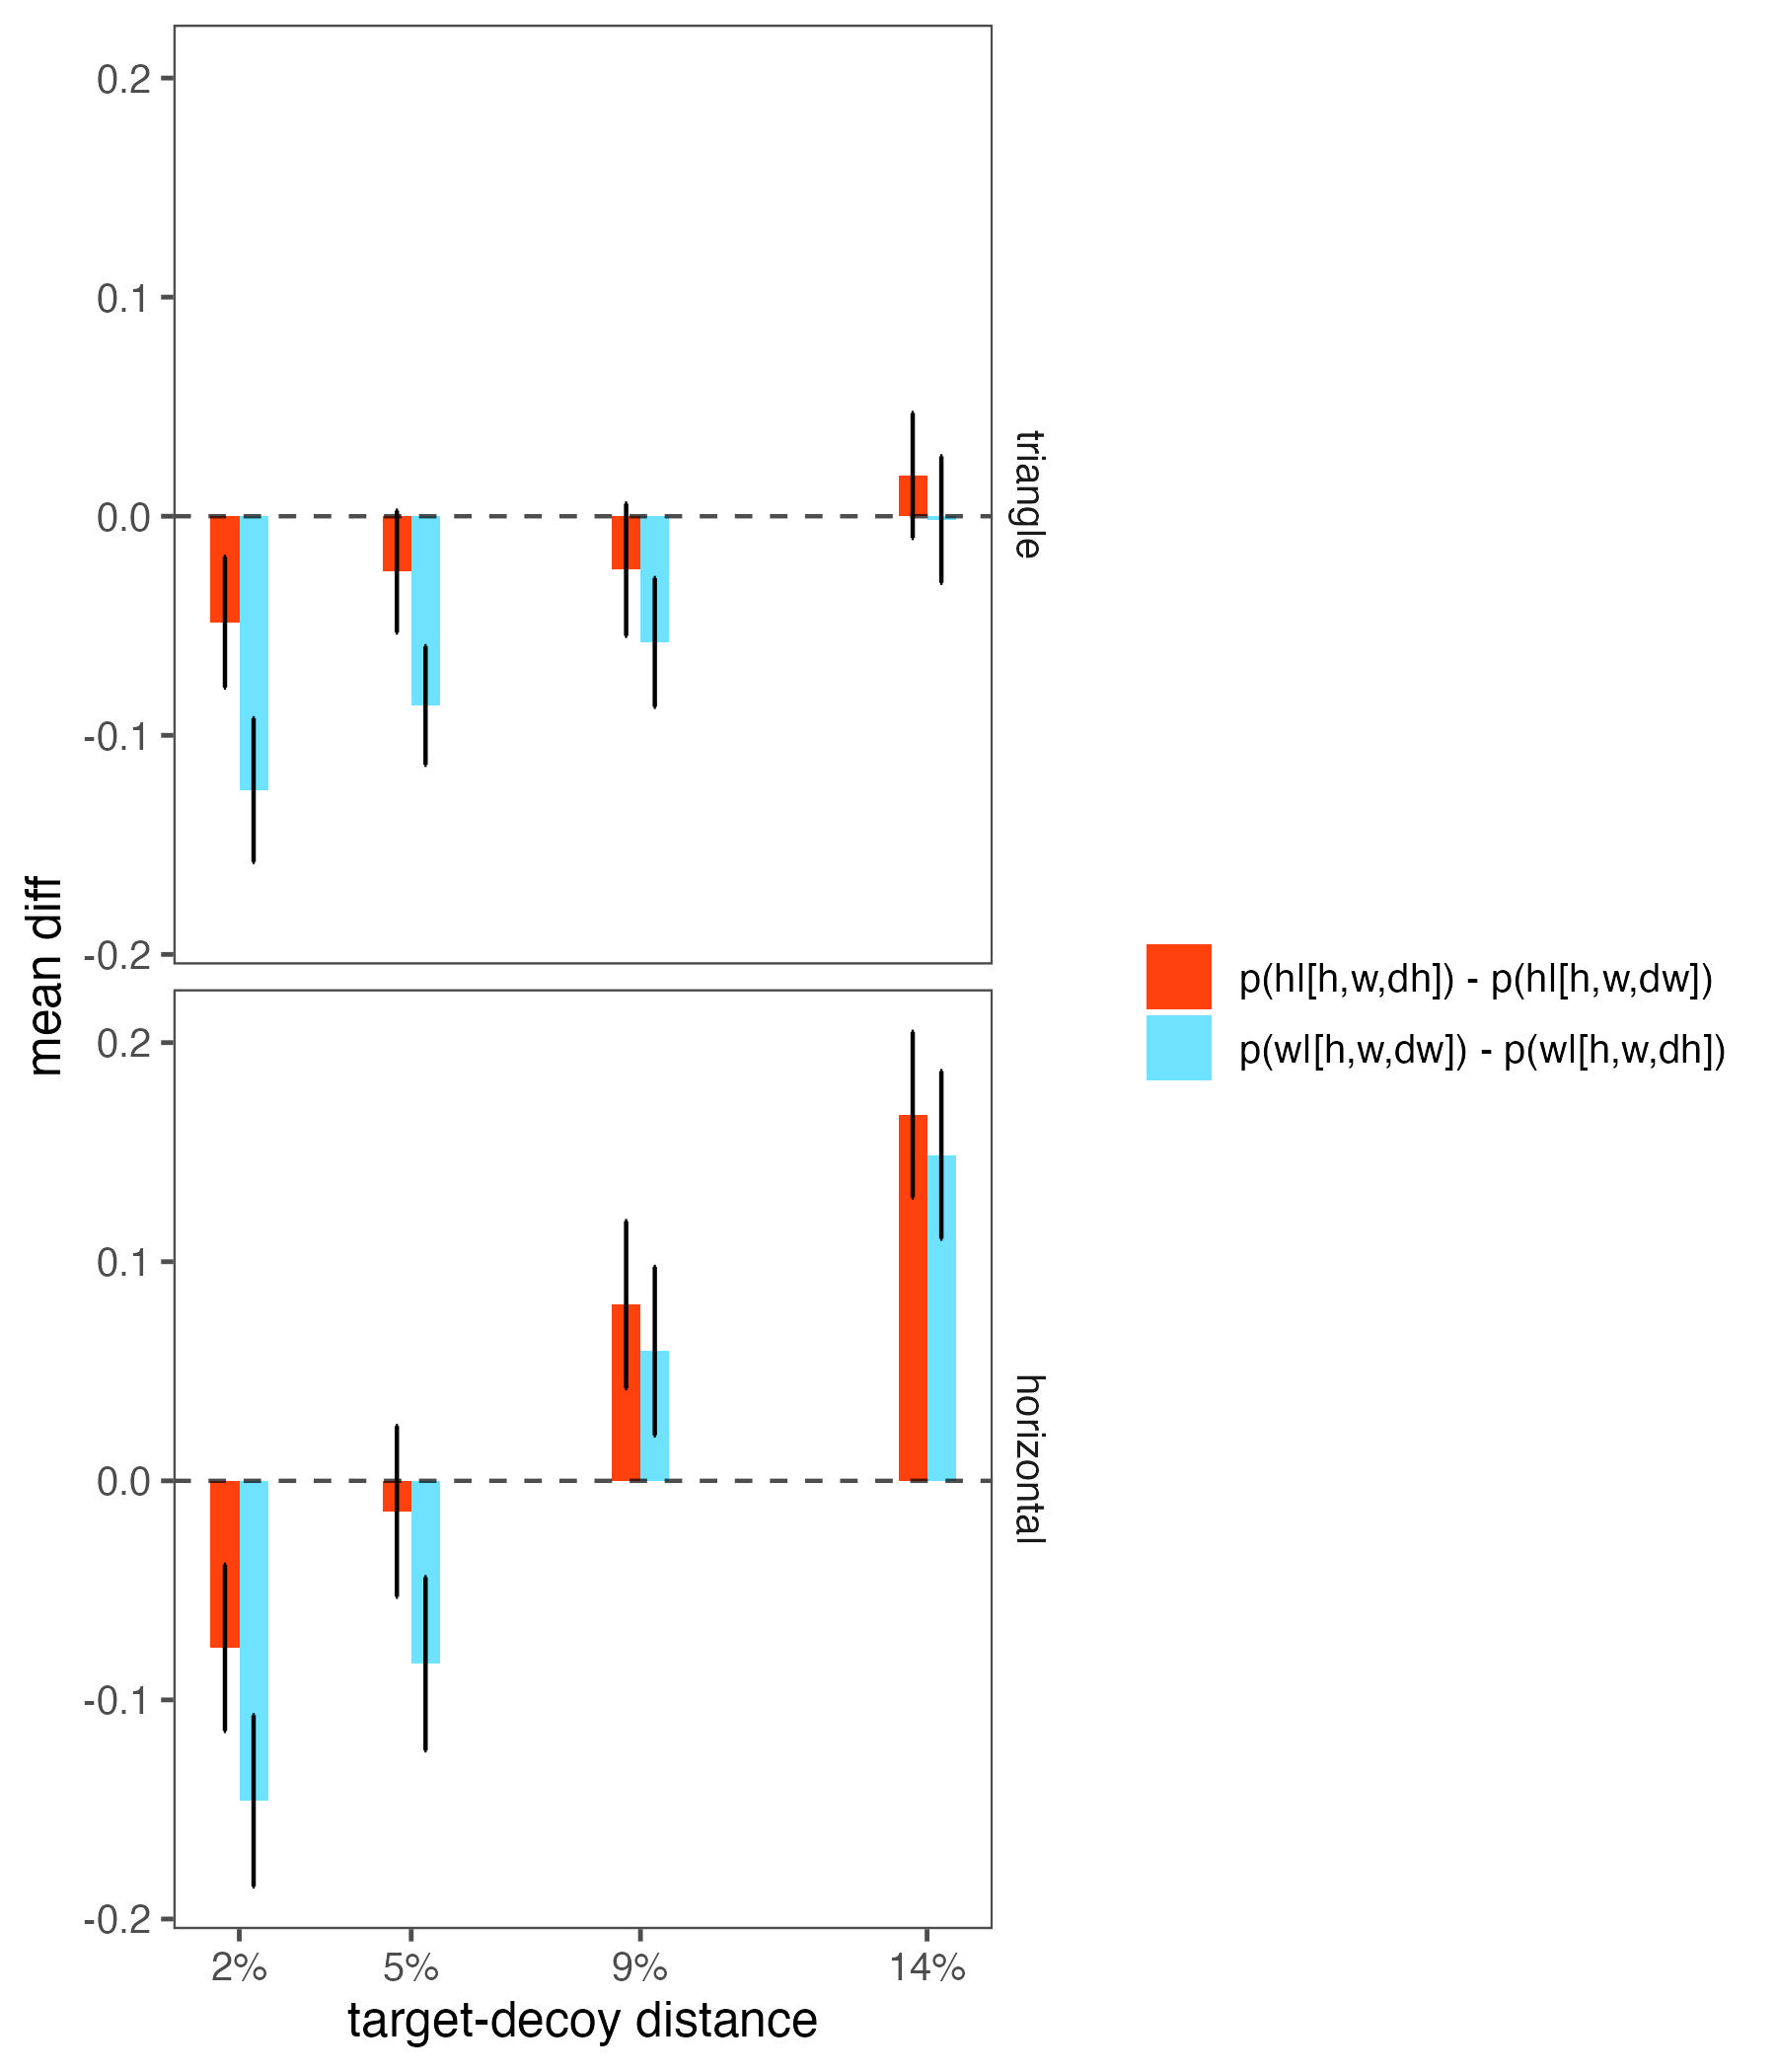
\includegraphics[width=\textwidth]{figures/choicePhase_delta_means.jpeg}
   \caption{Mean changes in choice proportions across choice sets. FIGURE IS ALSO A PLACEHOLDER}
   \label{e2_choicedeltas}
\end{figure}

\subsection{Model Simulations}
After estimating the parameters of the perceptual model and analyzing the choice data, I sought to test whether the model can predict the choice data. Though I showed in the introduction that this is possible, it was an open question whether the parameters estimated from actual data would produce qualitatively interesting predictions.

I used mean estimates of $\boldsymbol{\mu}$ and $\boldsymbol{\Sigma}$ (see the Appendix) to generate predictions at each level of TDD in both display conditions. I present the predictions in Figure~\ref{fig:e2_model_preds}. 

Given the estimated parameters, the model is able to produce a repulsion effect, but not an attraction effect. This aligns with our predictions from the introduction; the repulsion effect, at least in some forms, can be generated by a higher correlation between target and decoy stimuli compared to target-competitor and competitor-decoy pairs.

\subsection{Discussion}

The results of Experiments 1 and 2 show that participants are not always able to discriminate the decoy from the target and the competitor, and, that target-decoy perceptions appeared to be correlated. The observed correlations can, in turn, naturally produce the repulsion effect but not the attraction effect. 


Modern psychological models of context effects often assume an attribute-wise comparison process \parencite{roeMultialternativeDecisionField2001a,trueblood2013not,usherLossAversionInhibition2004a,bhatiaAssociationsAccumulationPreference2013b}. Under this class of models, participants arrive at a decision by comparing pairs of options on a single attribute, where the modeller assumes attribute values are veridical. This assumption is quite reasonable when modeling choices where each attribute is presented separately and discriminability issues are minimal or non-existent. In this article, I present evidence that this assumption may not be appropriate. ELABORATE HERE

\chapter{Extending a Perceptual Model to Best-Worst Choice}
\label{chapter_3}
\section{Introduction}

In Chapters 1 and 2, I presented a model of perceptual choice and showed it can systematically predict the repulsion effect, but not the attraction effect. In this chapter, I test another prediction of the model while demonstrating an important empirical result in another domain: best-worst choice.

\subsection{Introducing Best-Worst Choice}

Best-worst choice is an experimental paradigm where participants select their most and least preferred options from a choice set. Originally proposed by \textcite{finn1992determining}, best-worst choice is widely used in a number of applied fields, such as transportation \parencite{beck2016best} and healthcare economics \parencite{cheung2016using,flynn2007best,muhlbacher2016experimental}. One key advantage, when compared to traditional discrete choice research, is that researchers can use best-worst choices to gain information about participants' ranking of options while never requiring them to complete a full ranking task \parencite{marleyProbabilisticModelsBest2005}.

Researchers have developed theoretical models to account for best-worst choice data. Most best-worst choice models relate best-worst choices to an underlying utility function. \textcite{marleyProbabilisticModelsBest2005} developed a class of models known as the \textit{maxdiff} (maximum difference) models of best-worst choice\footnote{Note that the term maxdiff is sometimes erroneously used to refer to best-worst experiments in the generic sense. Following \textcite{marleyProbabilisticModelsBest2005}, I use maxdiff to refer to a specific class and parameterization of this choice model.}. According to the maxdiff model, given choice set $K$, the probability of selecting option $x$ as best and option $y$ as worst, where $x \neq y$, is defined computed as:

\begin{equation}
   BW_{K}(x,y)=\frac{e^{u_{x}-u_{y}}}{\sum_{\substack{{p,q}\in K\\p \neq q}} e^{u_{p}-u_{q}}}   
   \label{eqn:maxdiff_equation}
\end{equation}

where $u_{i}$ is the utility of option $i$, and $BW(x,y)$ indicates the probability of selecting $x$ as best and $y$ as worst. This model proposes that a single utility scale determines the selection of both the best option and the worst option in a choice set. It assumes that best-choice probabilities are an increasing function of $u$, while worst-choice probabilities are a decreasing function of $u$. The use of the exponential function means that the maxdiff model is another form of the widely used multinomial logit (MNL) choice model \parencite{hausman1984specification}. Utilities are also assumed to be independent.

There are several variants of this model along with other best-worst choice models \parencite{marleyProbabilisticModelsBest2005,marleyProbabilisticModelsSetdependent2008,marleyModelsBestWorst2012,flynnBestWorstScaling2007,flynn2014best}, though the maxdiff model from Equation~\ref{eqn:maxdiff_equation} remains the dominant model for analyzing best-worst choice data.

The maxdiff model predicts a monotonic relationship between best-choice probabilities and worst-choice probabilities \parencite{hawkinsBestTimesWorst2014}. Researchers have explored whether this monotonicity holds empirically. \textcite{hawkinsIntegratingCognitiveProcess2014a} examined both preferential and perceptual best-worst choice data using response time modeling. They used the linear ballistic accumulator model (LBA) \parencite{brownSimplestCompleteModel2008b}, which casts the decision process as a race between "accumulators" towards a threshold, where the average accumulation across trials is captured by the drift rate parameter. Modeling datasets containing both preferential and perceptual best-worst choice data, they were able to successfully account for choice data by assuming a parallel race between "best" and "worst" accumulators for each option. Furthermore, they showed that the utility values estimated for each option using a MNL model were positively linearly related to the log drift rate values from the LBA, suggesting an underlying utility representation that explains both types of choices. 

In a follow-up article, \textcite{hawkinsBestTimesWorst2014} found that, collapsing across choice sets, best-choice probabilities are monotonically related to worst-choice probabilities. Options that were most likely to be selected as best were least likely to be selected as worst, and vice versa. This finding held for perceptual choice and consumer choice. They also showed that, using the parallel best-worst LBA as a model, the drift rate parameter for worst choice can be parameterized as the reciprocal of the best choice drift rate. Formally, if $d_{b}(i)$ is the drift rate for selecting option $i$ as best, then $d_{w}(i)=1/d_{b}(i)$, where $d_{w}(i)$ is option $i$'s drift rate for worst choices. 

Both the parallel best-worst LBA and the maxdiff model assume that the utilities of all options presented are independent. However, as I show below, the perceptual model from Chapters 1 and 2 predicts, under certain conditions, a dissociation between best and worst choices inconsistent with this assumption.

\subsection{Model-Based Dissociations in Best-Worst Choice}

Here, I use the perceptual model to make a prediction regarding a dissociation between best choices and worst choices. 

Let $K$ be a choice set consisting of options $T$, $C$, and $D$ (i.e., target, competitor, and decoy). As in Experiments 1 and 2, the options are rectangles in a perceptual choice experiment. As in Chapter 2, I assume that on each trial $i$ with choice set $K$, the perceived area $\mathbf{X_{i}}$ of all 3 stimuli is sampled from a multivariate Gaussian distribution with a mean vector $\boldsymbol{\mu}$ and variance-covariance matrix $\boldsymbol{\Sigma}$ (see Equation~\ref{eqn:mvnorm}).

$\boldsymbol{\mu}$ and $\boldsymbol{\Sigma}$ are parameterized the same as in Chapters 1 and 2. 

Following conventions in the literature, I use $B(j)$ to denote the probability of selecting option $j$ as best and $W(k)$ to denote the probability of selecting option $k$ as worst. I also require the model (and participants in the experiment) to never select the same option as best and as worst.

I assume that, given a vector $\mathbf{X_{i}}$ of perceived areas on trial $i$ with set $K$, the probability a participant selects stimulus $j$ as best is:

\begin{equation}
   B(j|i,K)=P(\mathbf{X}_{ij}>\mathbf{X}_{ik}), \forall k \in K, j \neq k
   \label{eqn:bchoice1}
\end{equation}

while the probability of selecting stimulus $j$ as worst is:

\begin{equation}
   W(j|i,K)=P(\mathbf{X}_{ij}<\mathbf{X}_{ik}), \forall k \in K, j \neq k
   \label{eqn:wchoice1}
\end{equation}

Simply put, the option with the largest perceived area is always selected as best, while the option with the smallest perceived area is always selected as worst. 

As it happens, the correlations (i.e., $\Omega$) estimated from Experiment 2 predict that, in a best-worst choice paradigm, best and worst-choice probabilities are non-monotonically related. 

I computed predictions for best-worst choice by simulating the model using the mean parameters ($\boldsymbol{\mu}$ and $\boldsymbol{\Sigma}$) estimated from Experiment 2\footnote{I used only those estimated from the triangle condition (See Experiment 2).} and simulated a large number of trials ($N=1,000,000$). As in previous simulations, I collapsed over choice set (i.e., whether the target is wide or tall) and focused on target, competitor, and decoy choice proportions at each level of TDD. I present these results in Figure~\ref{fig:bw_sim}, in a series of state-trace plots \parencite{bamber1979state,ashby2022state}. In a state-trace plot, the analyst plots two dependent variables against one another in each experimental condition. 

\begin{figure}
   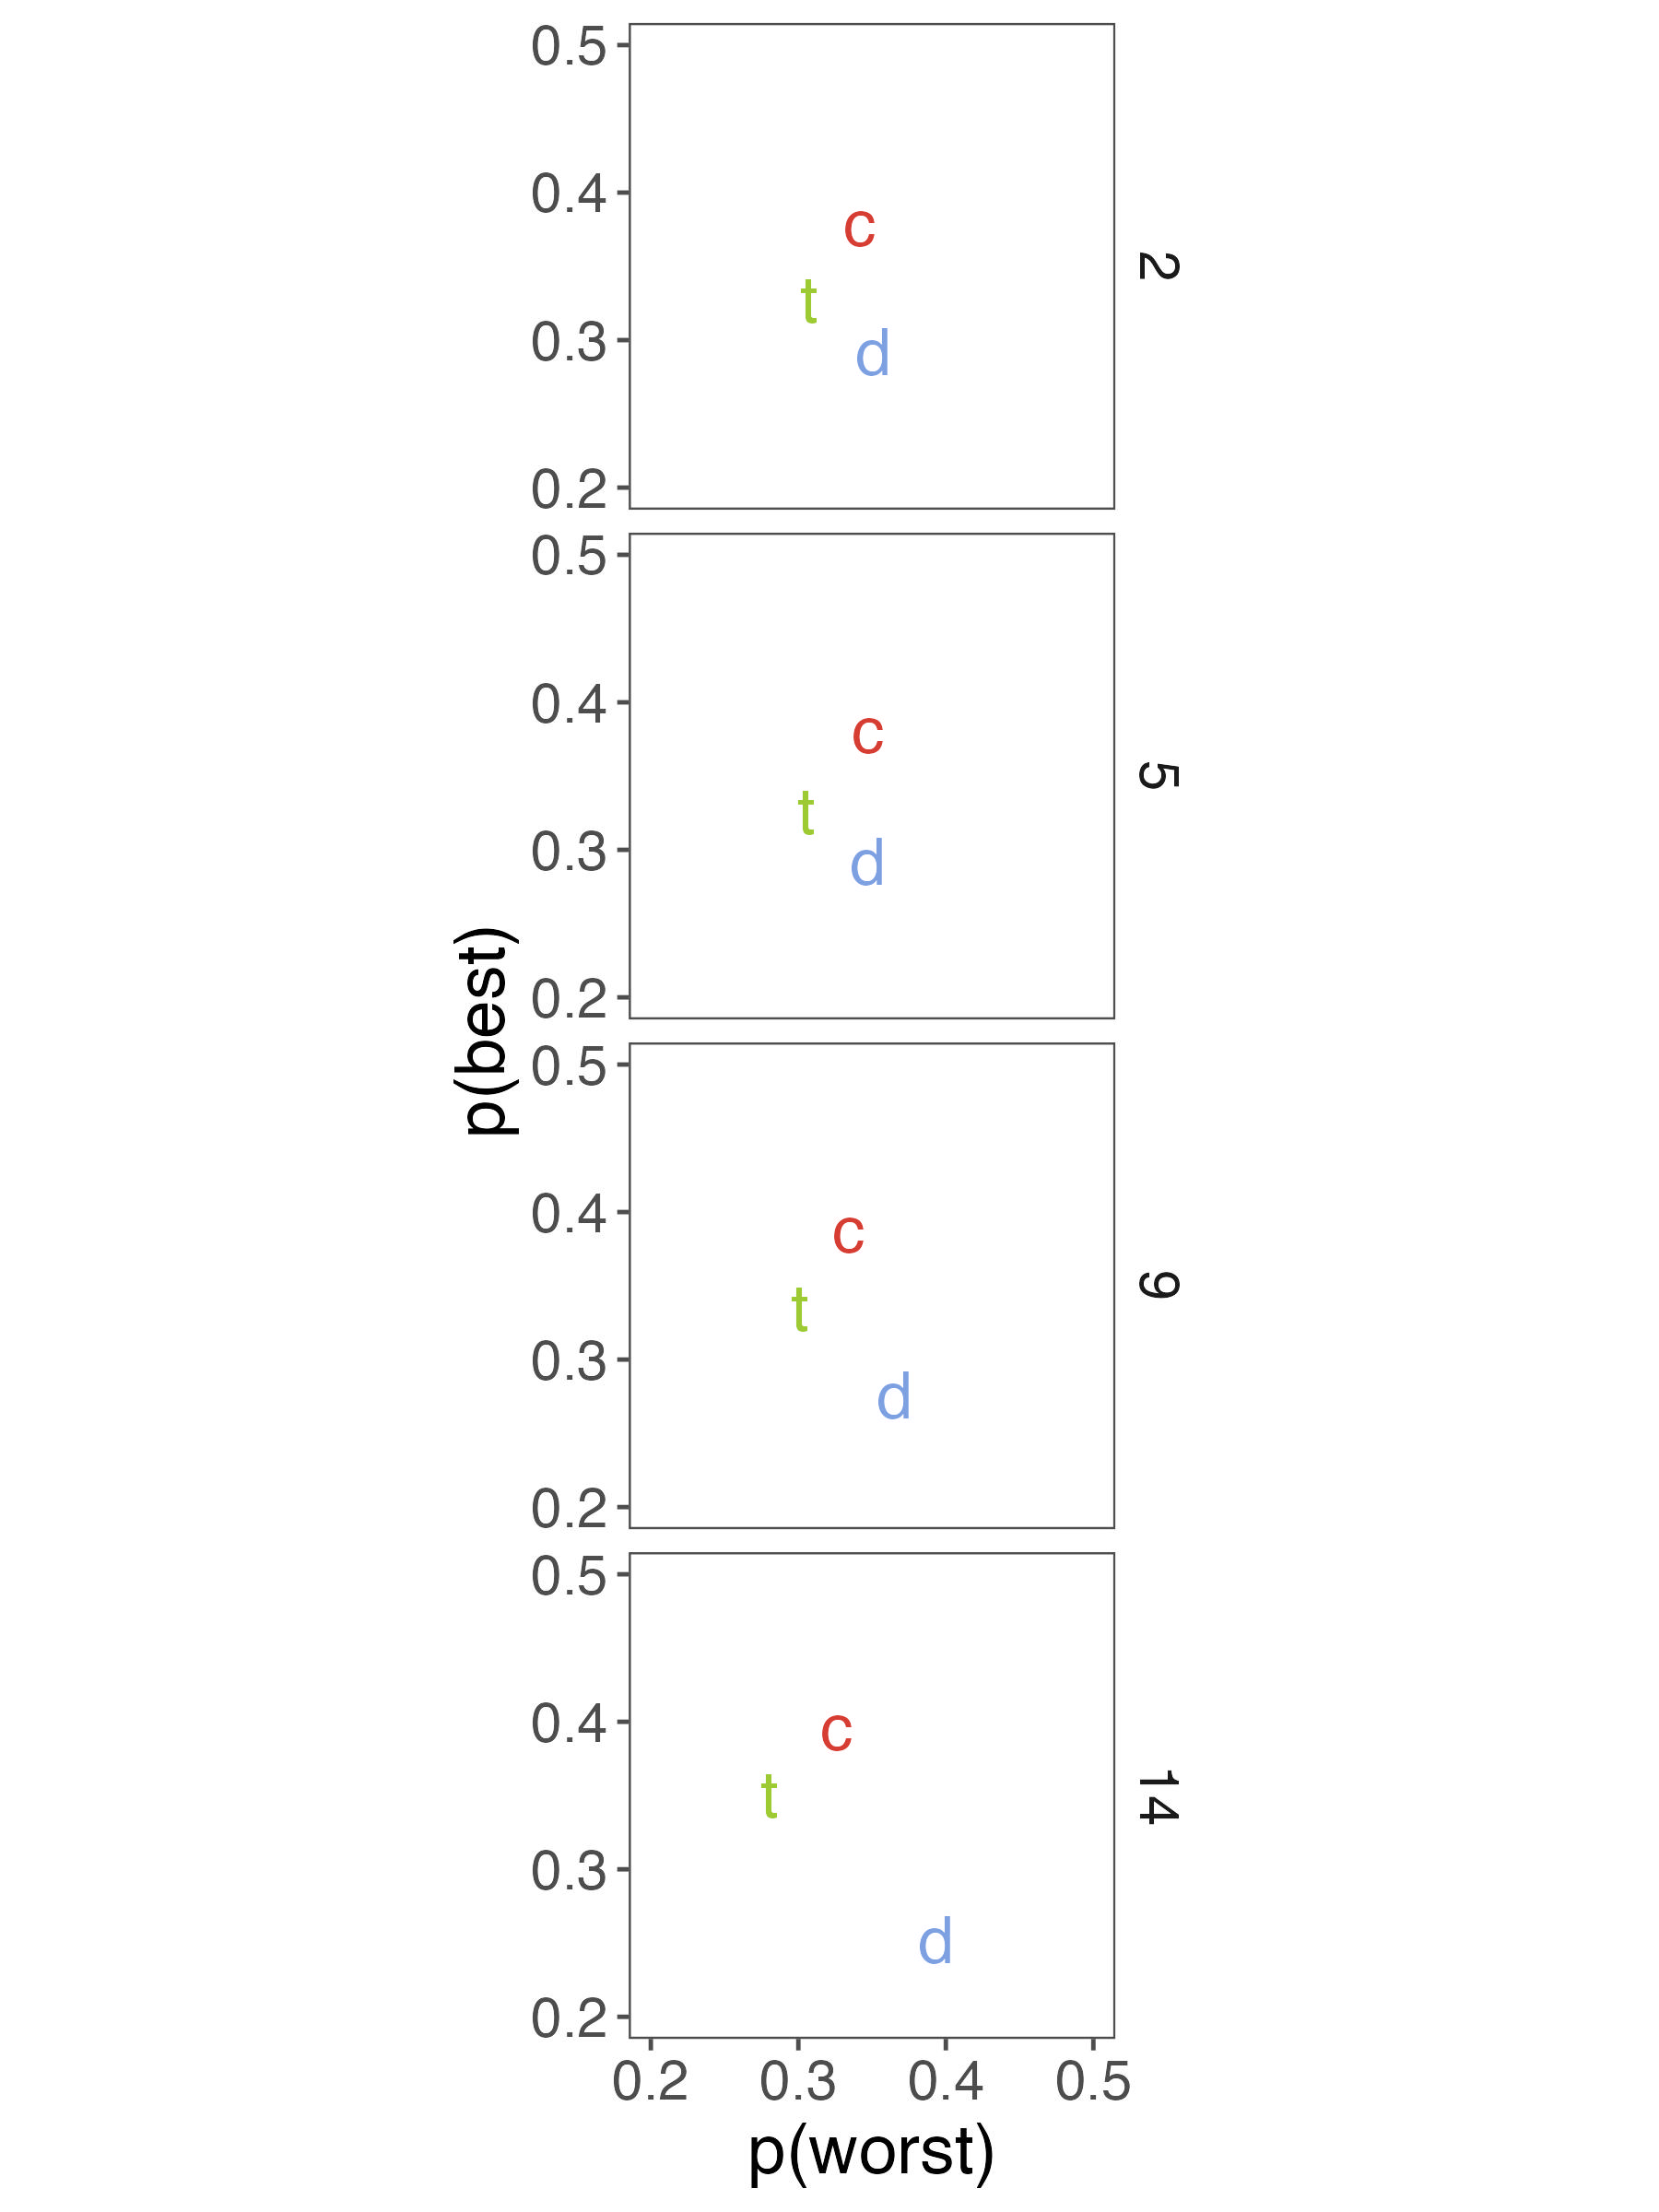
\includegraphics[width=\linewidth]{figures/bw_preds_sigma_constant_comp_effect_no_outliers.jpeg}
   \caption{Simulated best-worst predictions per the Thurstonian perceptual model. Each row is a different TDD value from Experiment 2.}
   \label{fig:bw_sim}
\end{figure}

The model, conditioned on the estimated parameters, predicts an interesting result. Although the competitor is most frequently chosen as best, due to the repulsion effect from Experiment 2 and from \textcite{spektorWhenGoodLooks2018b} Experiment 3, it is not, however, least frequently chosen as worst. Specifically, $B(C)>B(T)$, while $W(T)<W(C)$. At lower levels of $TDD$, the model even predicts that competitor and decoy are chosen at similar rates. As we will see, this prediction does not bear out empirically, and this prediction is likely due to the fact that participants are less sensitive to perceptual differences when providing ratings than when making choices \parencite{gronau2023choice}.

The Thurstonian perceptual model predicts this because $\rho_{TD}>\rho_{CD}\approx\rho_{TC}$. On the (relatively few) trials where $X_{iD}$ is largest, it is more likely that $X_{iD}>X_{iT}>X_{iC}$ than $X_{iD}>X_{iC}>X_{iT}$. In other words, the high $\rho_{TD}$ value "pulls up" the target more than the competitor. The similarity, and comparability, of target and decoy entail that the repulsion effect at the best-choice level (Experiment 2) does not necessarily show up at the worst-choice level.

The maxdiff model predicts a monotonic state-trace plot. That is, if we assume all options' utilities are independent, the model predicts that best-choice probabilities are negatively related to worst-choice probabilities. To demonstrate this, I simulated the maxdiff model using randomly generated independent utilities. See Figure~\ref{fig:maxdiff:sim}. 

\begin{figure}
   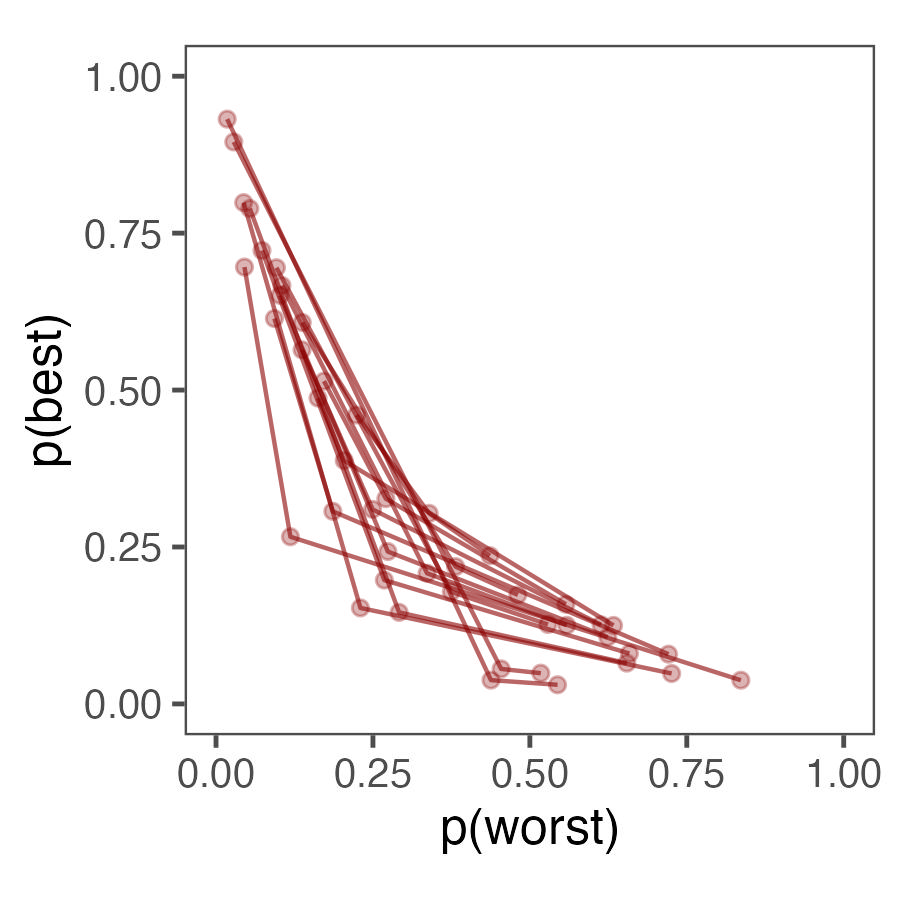
\includegraphics[width=150mm]{figures/maxdiff_sim_monotonic.jpeg}
   \caption{Best-worst choice simulations using the maxdiff model. Each curve is a separate simulation. The model predicts a negative, monotonic relationship between best-choice and worst-choice.}
   \label{fig:maxdiff_sim}
\end{figure}

This effect is subtle, and the predicted effect size is small. Indeed, all differences in predicted $W(C)-W(T)$ values were $<.05$. In Experiment 3, I show the empirical and modeling results from a best-worst choice experiment designed to test this prediction. I show that the dissociation between best and worst choices does indeed occur. I also show that the assumption of monotonicity required by the maxdiff model can fail empirically.

\section{Experiment 3}

The goal of Experiment 3 was to test the predictions of the Thurstonian perceptual choice model. Specifically, the perceptual model predicts that $B(C)>B(T)$ but $W(T)<W(C)$. To test this prediction, I used stimuli identical to those of Experiment 2 and presented stimuli in the triangle display of Experiments 1 and 2.
I show that 1) this prediction holds empirically and 2) the maxdiff model cannot account for these results, even when all parameters are free to vary. 

\subsection{Methods}

\subsubsection{Participants.}
Data collection took place at the University of Massachusetts Amherst. $392$ undergraduate students participated in exchange for course credit. $23$ participants who achieved less than $80\%$ accuracy on catch trials (see below) were excluded from all analyses. Trials with response times (RTs) $<100\text{ms}$ or  $>10000\text{ms}$ were also excluded from all analyses.

\subsubsection{Stimuli.}
The experiment had three types of trials: critical trials, filler trials, and catch trials. 

Stimuli on critical trials were identical to those of Experiment 2. On each critical trial, the target and competitor had the same area but differed on orientation, with one stimulus being wide and the other tall. The decoy always had the same orientation as the target. I varied TDD at $2\%$, $5\%$, $9\%$, and $14\%$. I also varied the target, competitor, and decoy rectangles along three diagonals, as in Experiment 2. 

On each filler trial, three stimuli were uniformly sampled from the space between the largest and smallest diagonals.

On each catch trial, one stimulus was sampled from the largest diagonal, while two stimuli were sampled from the smallest diagonal.

\subsubsection{Design.}
There were 8 blocks of trials. In each block there were 24 critical trials, 6 at each TDD level. There were 8 trials per diagonal. In addition to the critical trials, there were 10 filler trials and 3 catch trials per block.

Participants were randomly assigned into one of two conditions: best-worst or worst-best. On each trial, participants in the best-worst condition initially chose the largest rectangle and then chose the smallest rectangle. Participants in the worst-best condition chose in the opposite order. The condition factor was included to account for the possibility that best-worst choice order impacts choice. Results were consistent regardless of condition, so I collapsed over this factor in the analyses reported below.

After removing participants, there were 185 participants in the best-worst condition and 184 participants in the worst-best condition.

Stimuli were presented on computer monitors with a resolution of 1920 x 1080 pixels. The experiment was programmed with GNU Octave and Psychtoolbox \parencite{octave,brainardPsychophysicsToolbox1997}. 

\subsubsection{Procedure.}

The experiment began with three practice trials, which were identical to the filler trials. 

On each trial, participants saw three rectangles, labeled 1, 2, and 3 (from left to right), arranged in a triangle display. Participants in the best-worst (worst-best) condition saw a prompt asking them to select the largest (smallest) rectangle on screen. Participants used the mouse to click on their chosen rectangle. After they made their choice, this rectangle changed color to indicate that it was no longer available as an option. Next, participants in the best-worst (worst-best) condition selected the smallest (largest) rectangle, at which point the trial ended. See Figure~\ref{fig:bw_example_trial} for an example trial.

\begin{figure}
   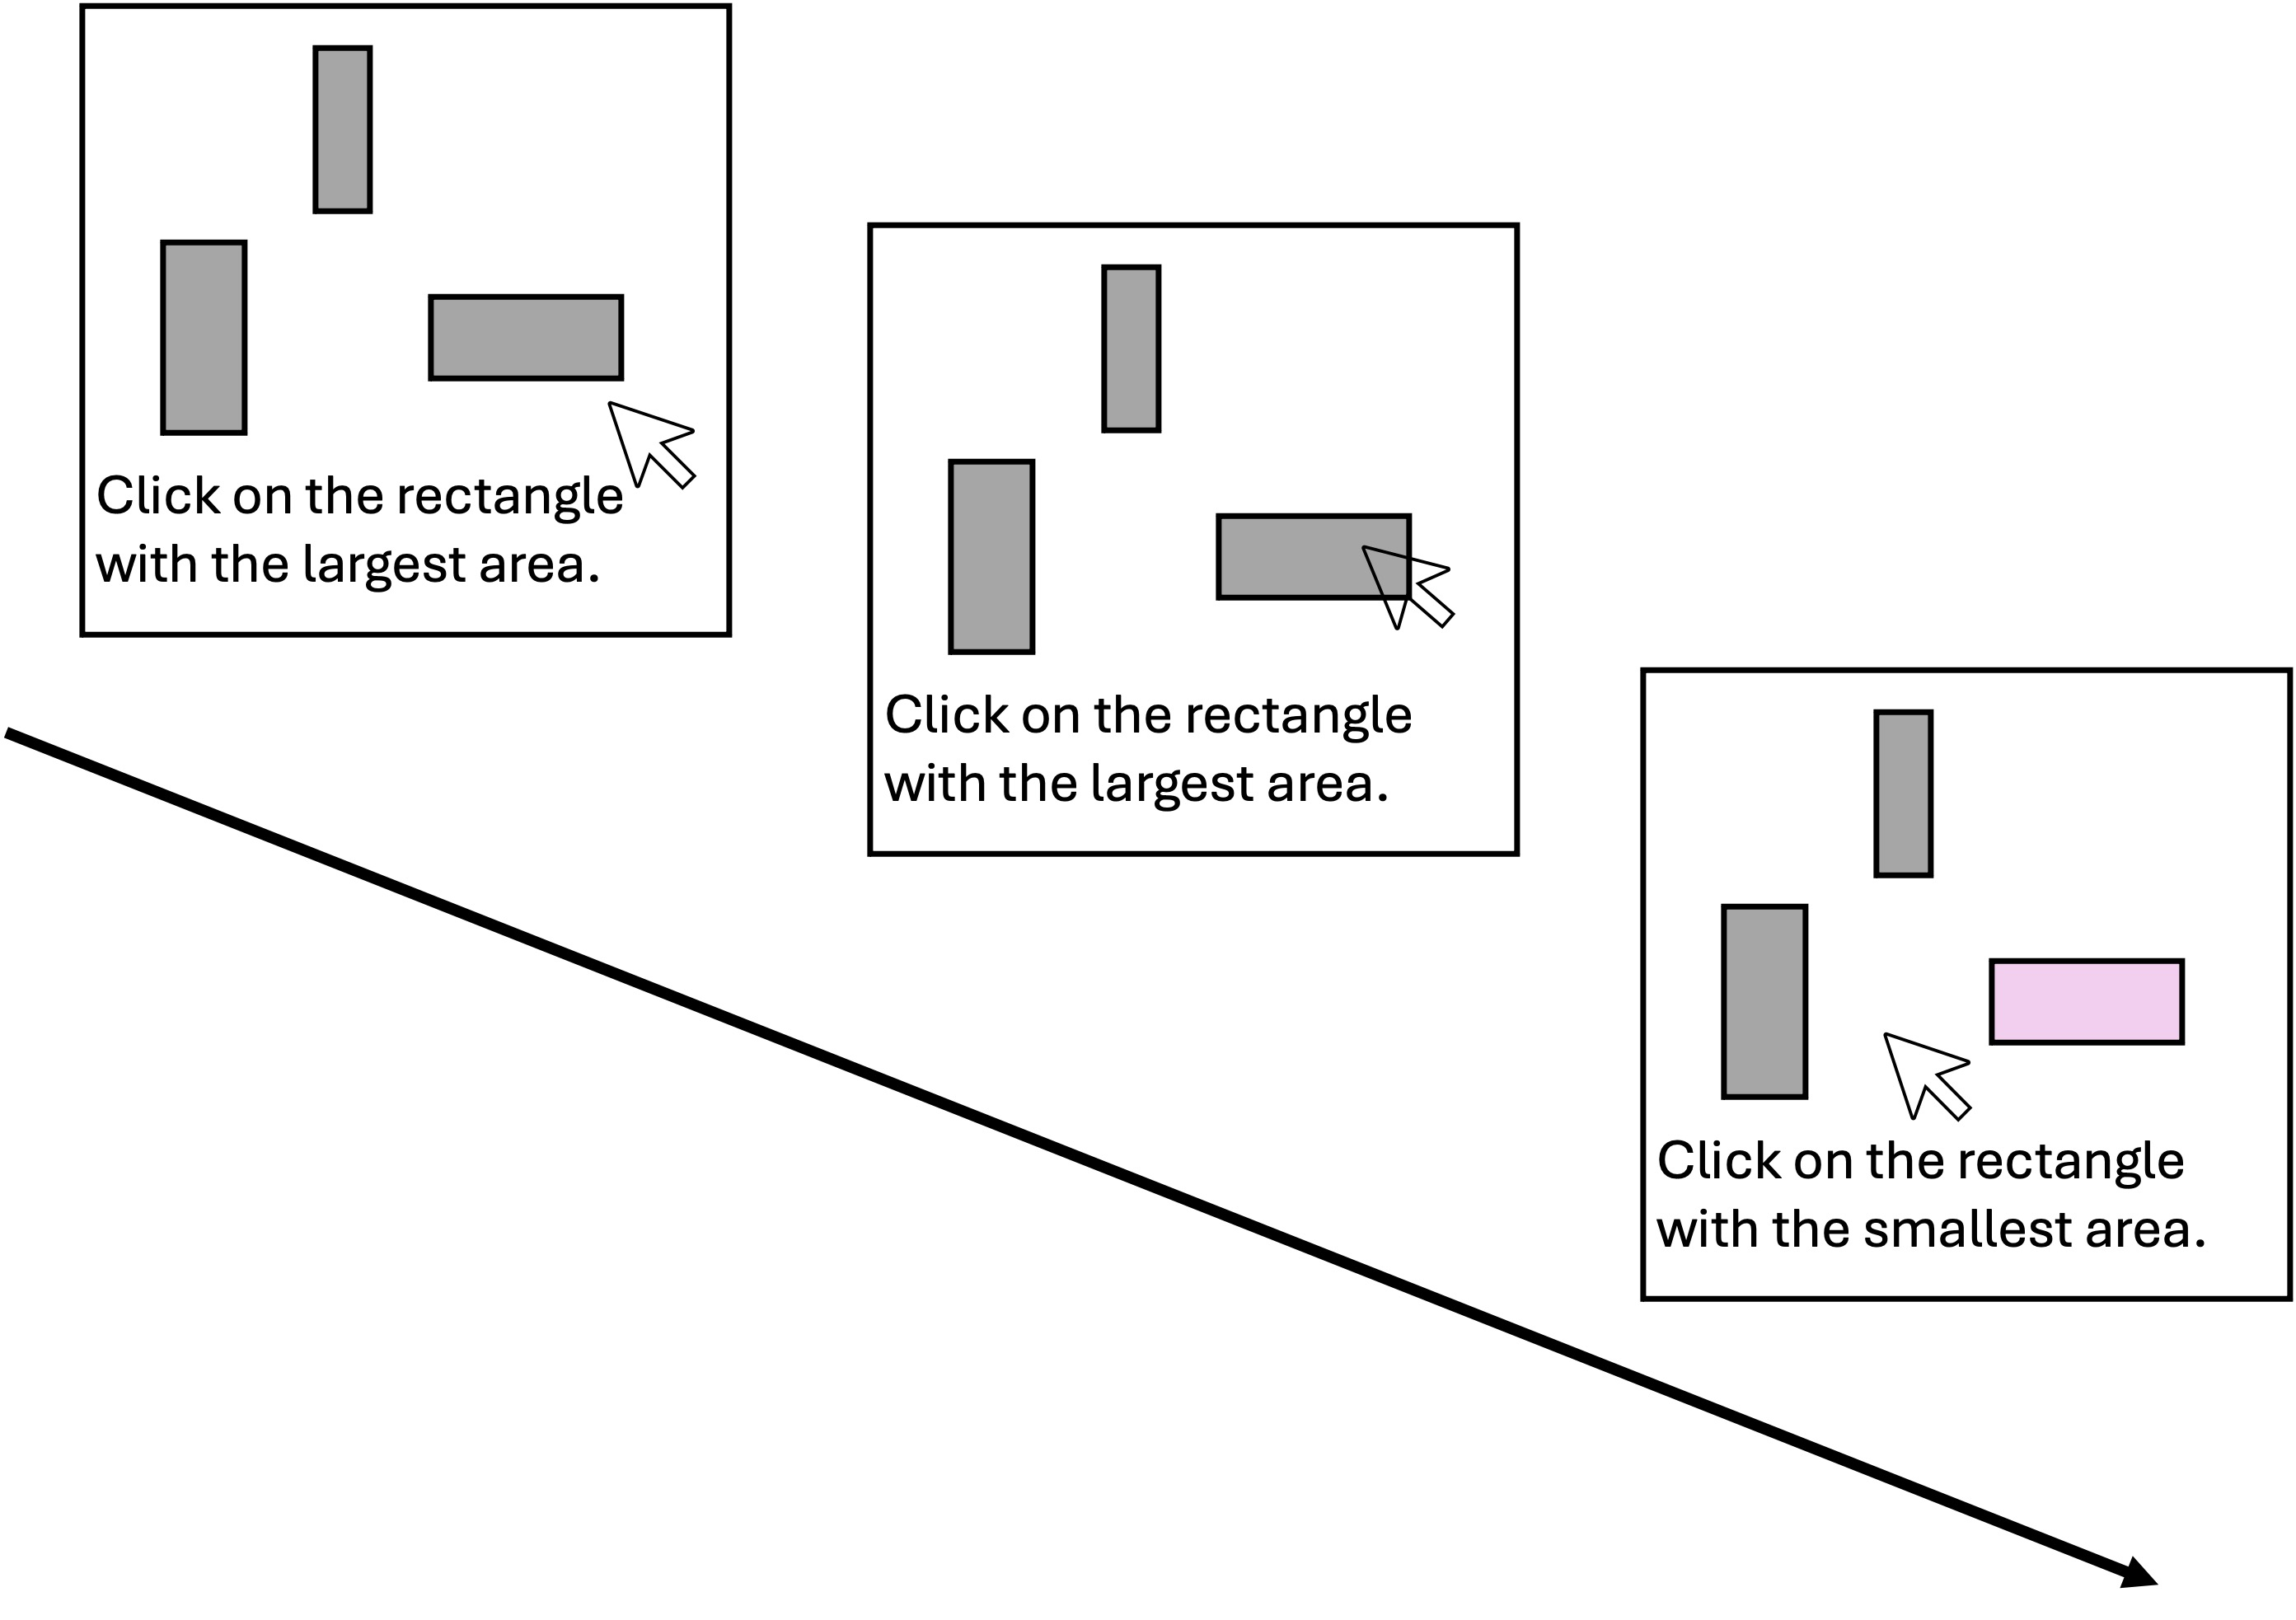
\includegraphics[width=\linewidth]{figures/bw_design_fig.jpg}
   \caption{A sample experimental trial from Experiment 3. Note that this is a trial in the best-worst condition.}
   \label{fig:bw_example_trial}
 \end{figure}
 
Stimulus order was randomized on each trial. 

Participants were told their percentage correct of best choices, worst choices, and overall choices at the end of the experiment.

\subsection{Results}


\subsubsection{Catch Trials.}
Participants performed well on the catch trials. The mean percentage correct for best choices was $97.97\% (SD=14.09)$, and the mean percentage correct for worst choices was $98.26\% (SD=13.09)$. The mean percentage correct for both best and worst choices (i.e., the mean percentage of the trials on which participants were able to correctly identify the largest and smallest rectangles) was $96.98\% (SD=17.12)$. 

\subsubsection{Filler Trials.}
Participants performed worse on the filler trials compared to the catch trials, but still well above chance. The mean percentage correct for best choices was $89.83\% (SD=30.23)$, and the mean percentage correct for worst choices was $88.95\% (SD=13.09)$. The mean percentage correct for both best and worst choices was $96.98\% (SD=17.12)$. 

\subsubsection{Critical Trials.}

First, I computed the mean choice proportions for each distinct rectangle, collapsed across choice set. Here, I replicated the findings of \textcite{hawkinsBestTimesWorst2014}, that, when ignoring the effect of context, best choices and worst choices are monotonically related. These data are plotted in Figure~\ref{fig:bw_marginal}.

\begin{figure}
   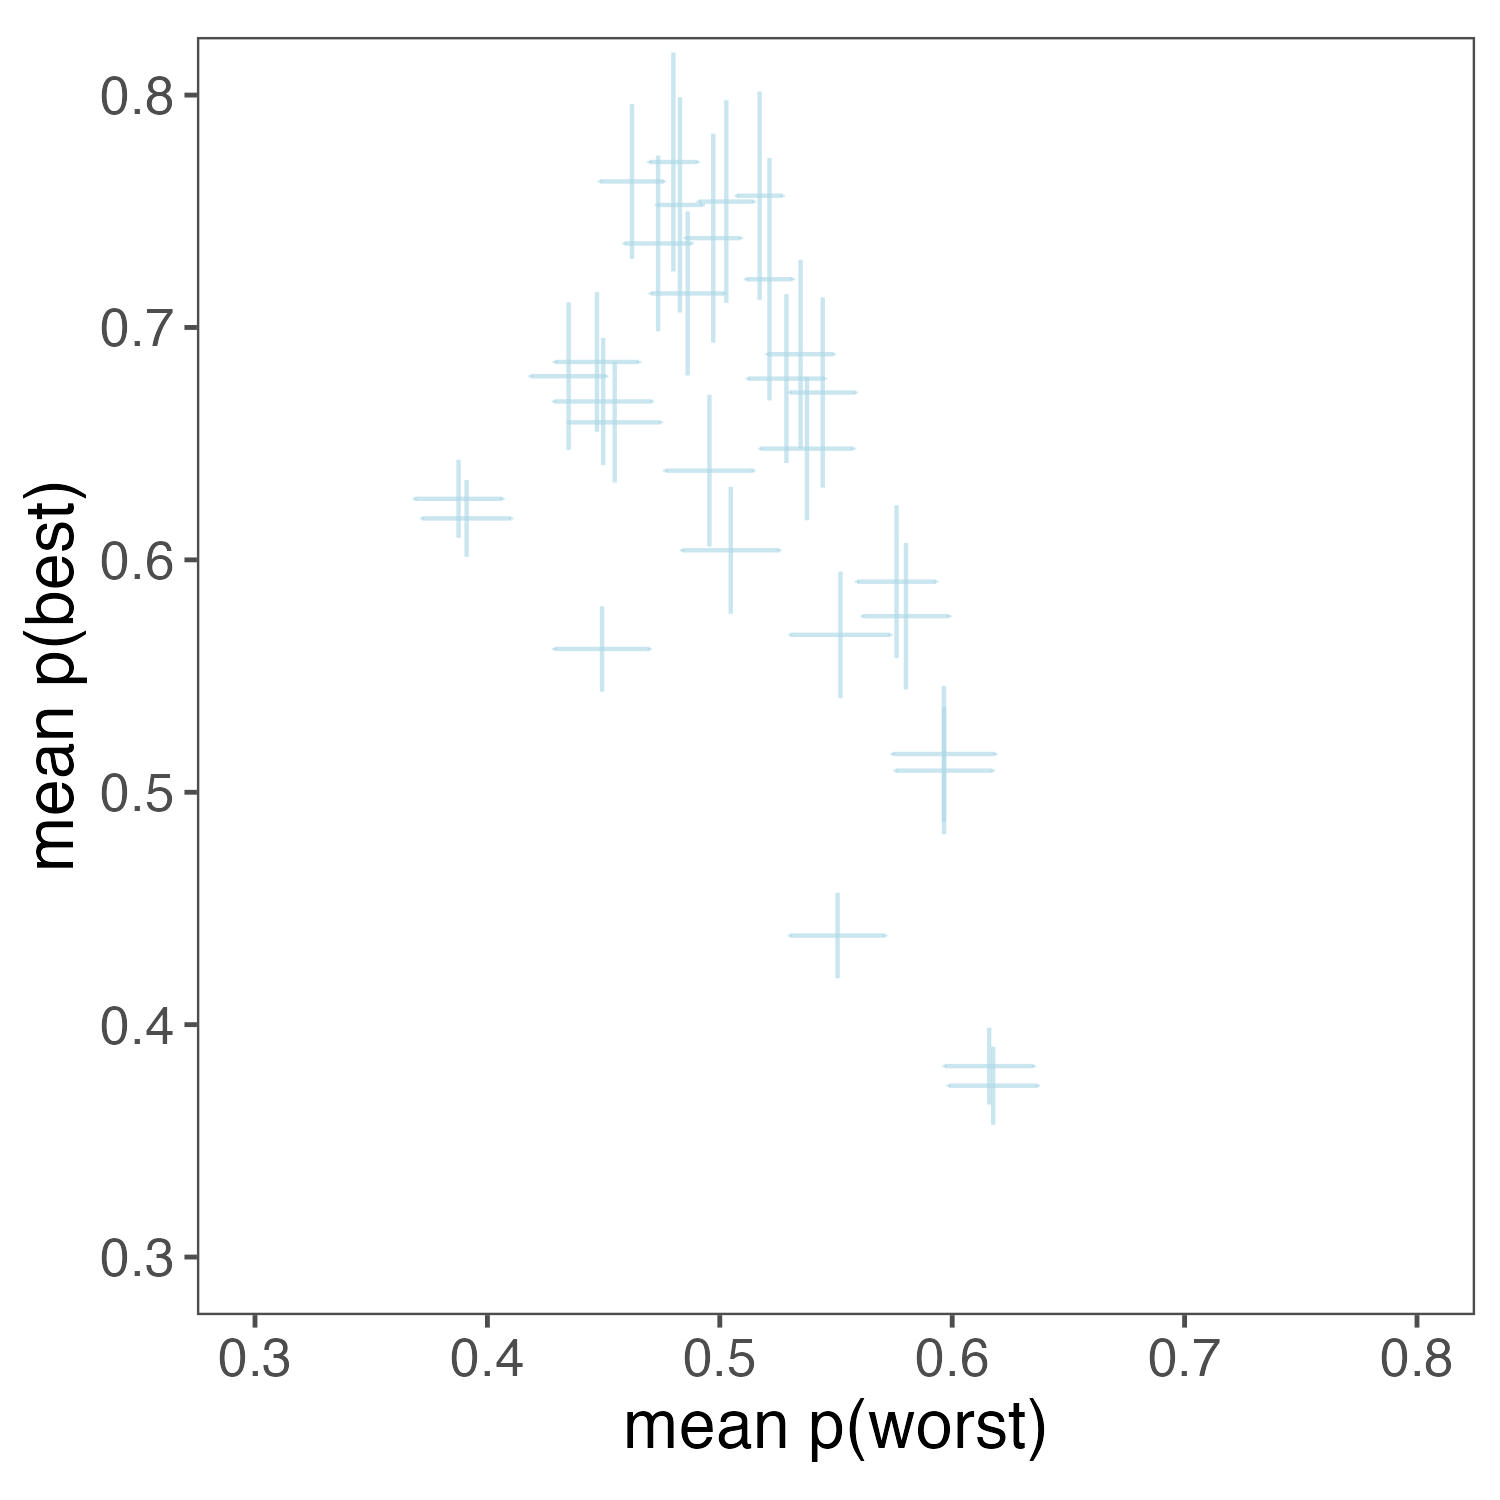
\includegraphics[width=\linewidth]{figures/crit_mean_props_marginal.jpeg}
   \caption{Experiment 3 marginal mean best and worst-choice proportions for all unique rectangles, collapsed across choice set. X and Y axis error bars are $95\%$ CIs.}
   \label{fig:bw_marginal}
\end{figure}

Next, I analyzed choice proportions by conditioning on TDD and choice set. Mean choice proportions for these data are plotted in Figure~\ref{fig:bw_mean_choice_by_set}. 

\begin{figure}
   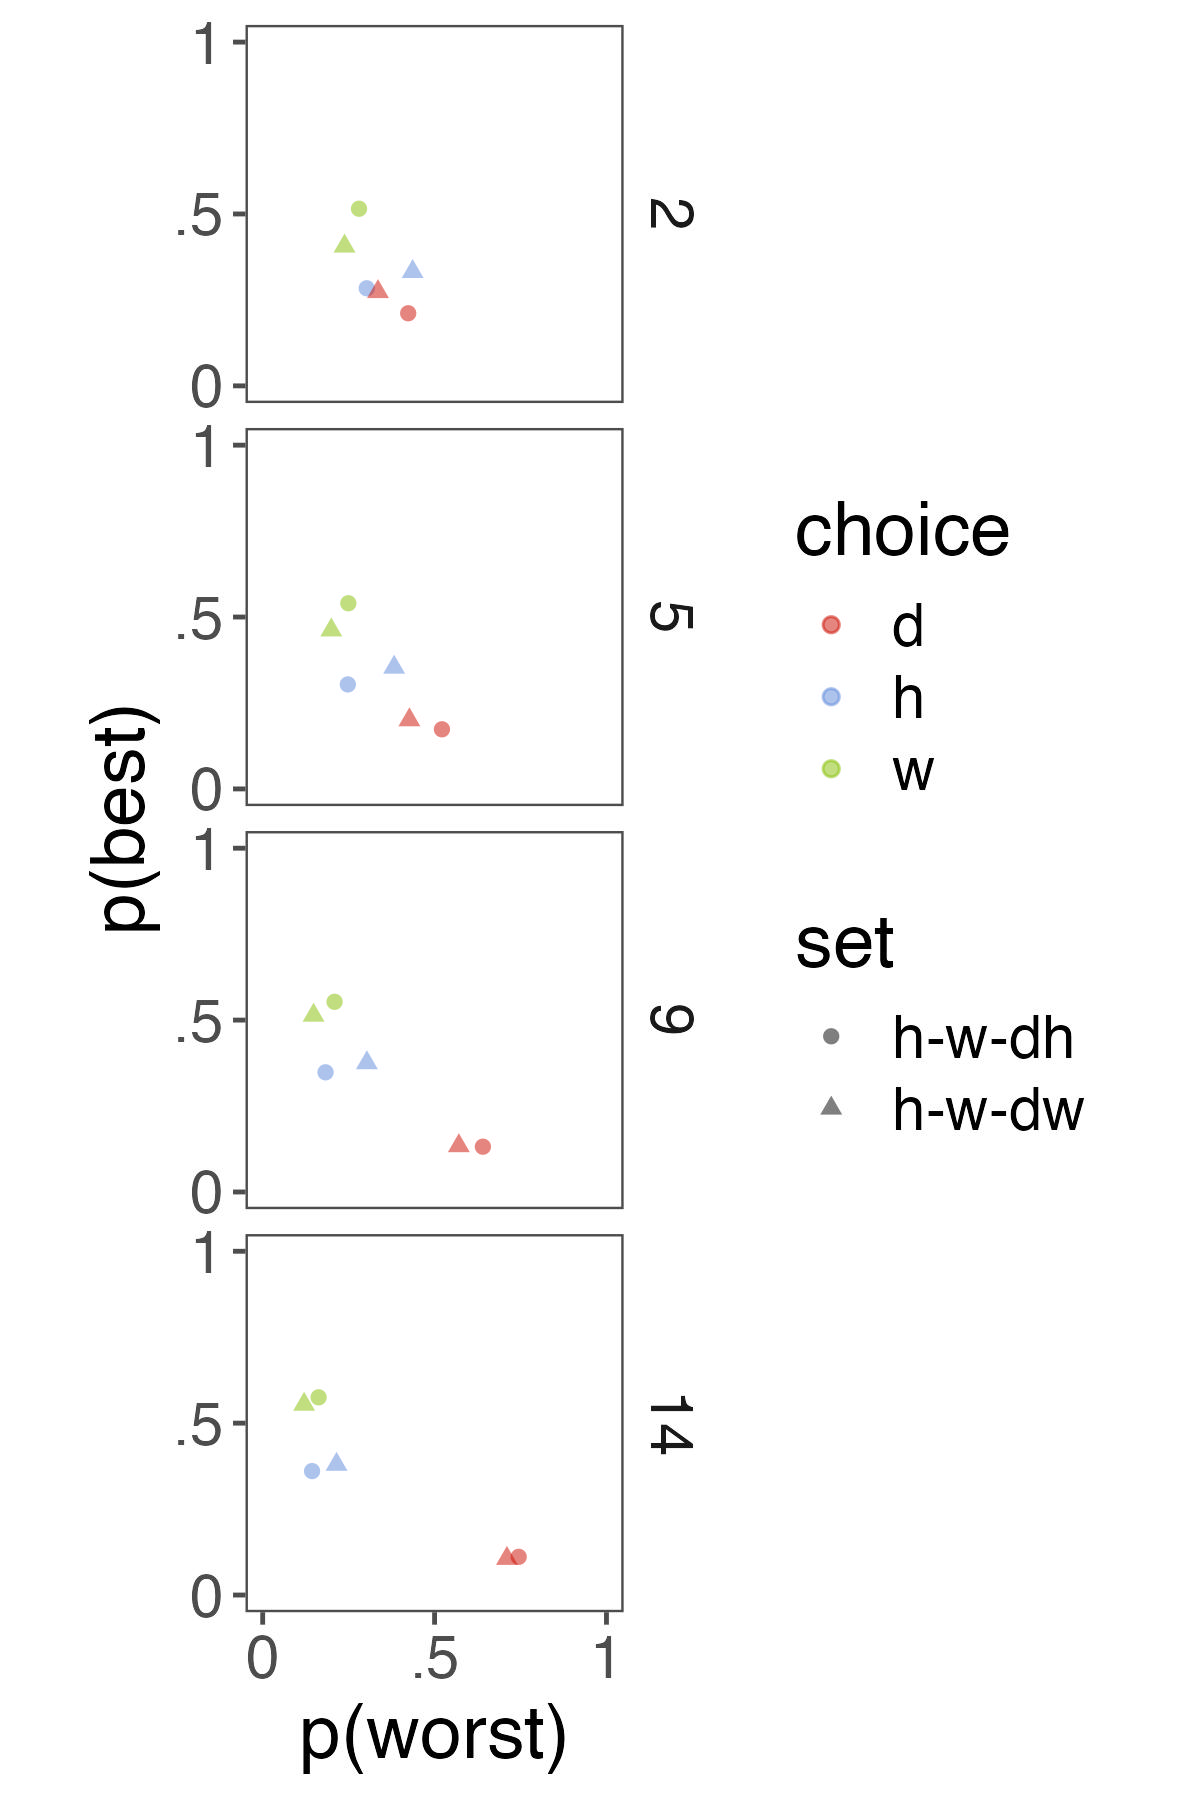
\includegraphics[width=100mm]{figures/crit_mean_choice_by_set_dist_labelHW.jpeg}
   \caption{Experiment 3 mean best and worst-choice proportions for the $h$, $w$, and $d$ rectangles, conditioned on TDD (rows) and choice set (shapes).}
   \label{fig:bw_mean_choice_by_set}
\end{figure}

Participants showed a consistent bias to choose $w$ (the wider rectangle) as largest, a finding also shown in Experiments 1 and 2. Participants also (on average) regularly choose the decoy rectangle as smallest, with the exception of the choice set $h,w,d_{w}$ and $TDD=2\%$, where they selected the $h$ rectangle as smallest, on average. This can be attributed to the difficulty of the $TDD=2\%$ condition and the overall wide rectangle bias. However, consistent with the predictions of the model, the target was still less likely to be chosen as worst than the competitor, $W(h|{h,w,d_{h}})<W(h|{h,w,d_{w}})$ and $W(w|{h,w,d_{w}})<W(w|{h,w,d_{h}})$, while the competitor option was more likely to be chosen as best, $B(h|{h,w,d_{w}})>B(h|{h,w,d_{h}})$ and $B(w|{h,w,d_{h}})>B(w|{h,w,d_{w}})$. 

These results are more easily understood by plotting mean target, competitor, and decoy choice proportions across TDD levels, collapsed over choice set. See Figure~\ref{fig:bw_mean_choice_collapsed} for these data. 

The best-choice proportions replicated the repulsion effect initially found by \textcite{spektorWhenGoodLooks2018b} and replicated in Experiment 2, where the competitor was more likely to be chosen as best at low TDD levels, while the target and competitor were chosen equally often at high TDD levels. Decoy best-choice proportions also decrease systematically with TDD. 
% See the Appendix for inferential statistics which support these conclusions.

Furthermore, the target is always more likely to be chosen as worst, compared to the competitor and decoy, at all TDD levels, $W(T)<W(C)$, as predicted by the perceptual model outlined in Chapter 2. This model still cannot predict the null best-choice repulsion effect when $TDD=14\%$, as discussed in Chapter 2, which suggests that this effect may be due to higher level decision processes.

\begin{figure}
   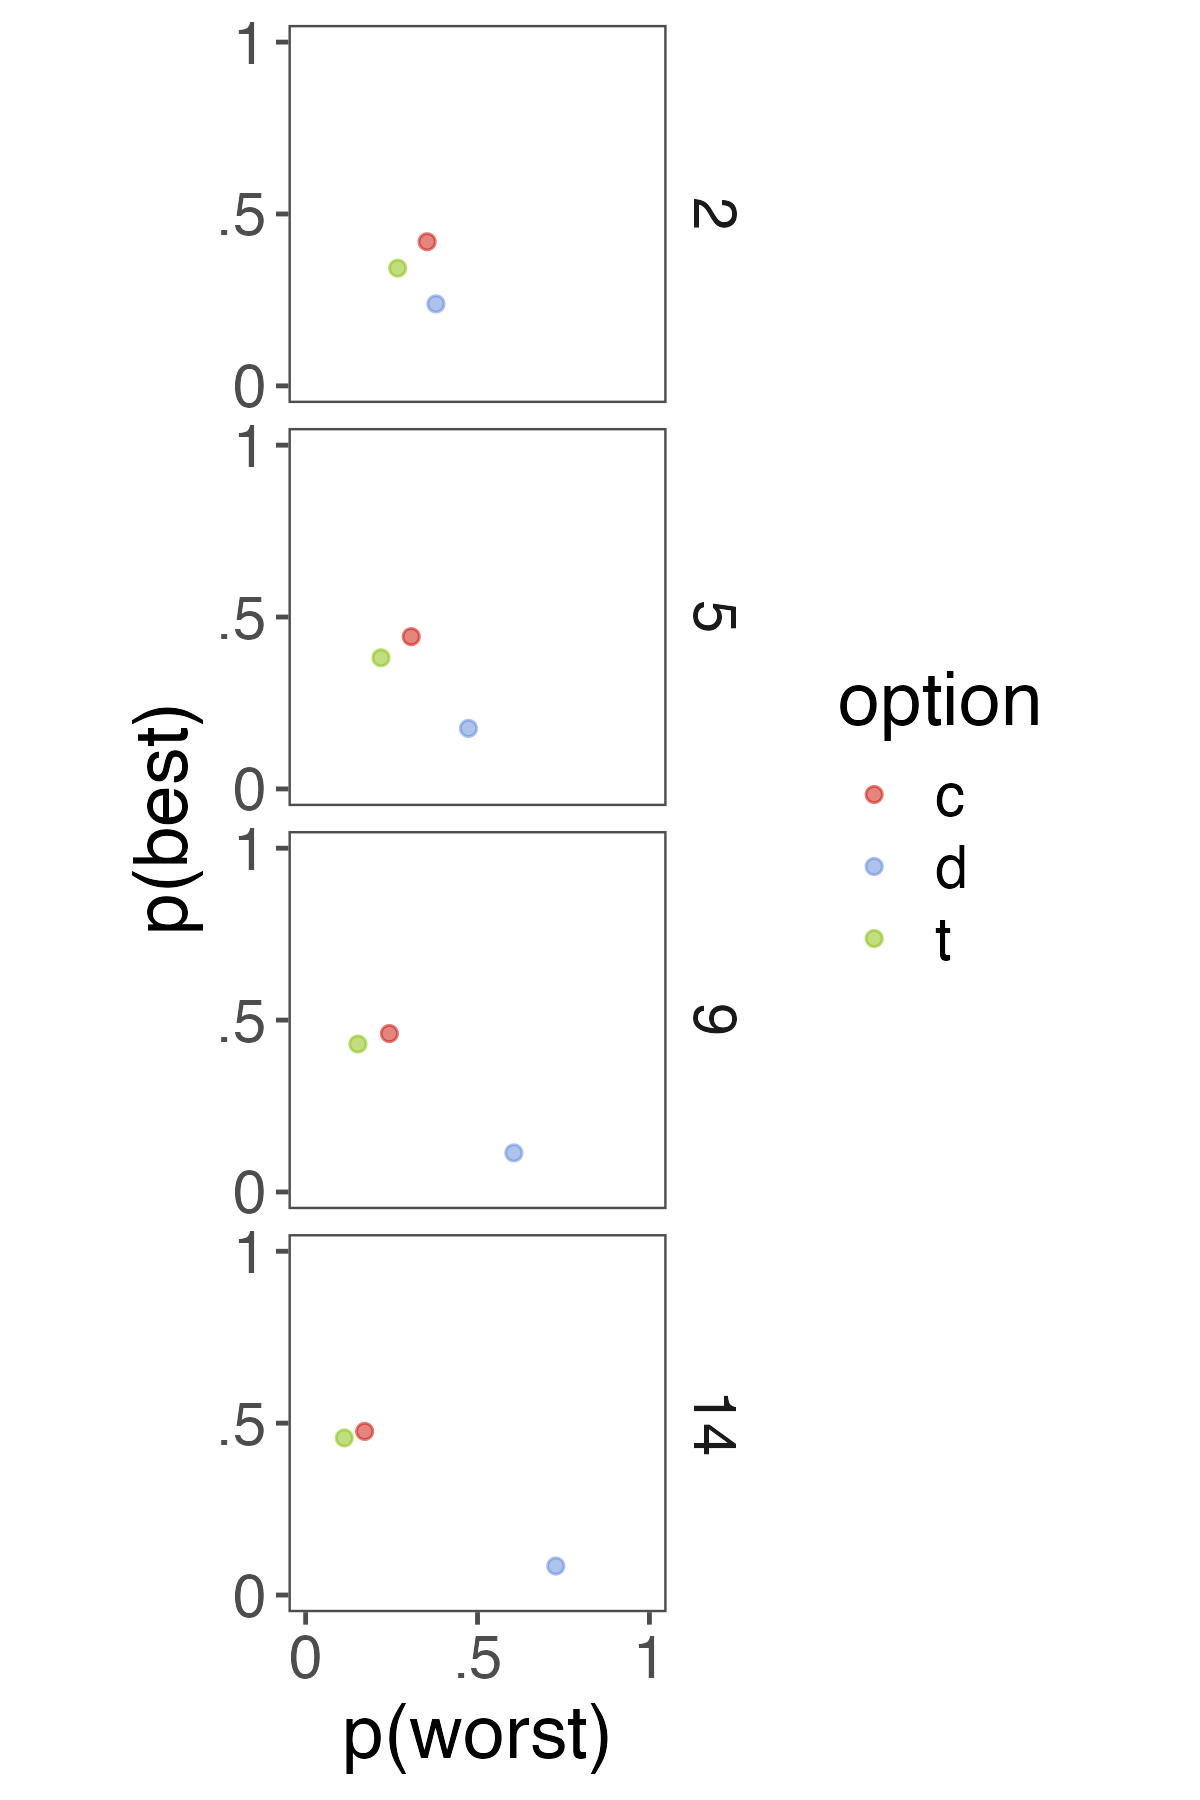
\includegraphics[width=100mm]{figures/crit_mean_props_by_dist.jpeg}
   \caption{Experiment 3 mean best and worst-choice proportions for the target, competitor and decoy rectangles, conditioned on TDD (rows).}
   \label{fig:bw_mean_choice_collapsed}
\end{figure}

\subsubsection{Maxdiff Modeling}

I first turn to the maxdiff model \parencite{marleyProbabilisticModelsBest2005}, which was outlined in the introduction to this chapter. This equation predicts that the probability of choosing options $x$ as best and $y$ as worst, $x \neq y$, increases monotonically with the difference in their estimated utilities (see Equation~\ref{eqn:maxdiff_equation}). This model is the most commonly used analysis technique for best-worst choice data. I applied this model to the current experiment and show that it is unable to predict the observed dissocations in best-worst choices, even with its best fitting parameters.

I implemented this model as a Bayesian hierarchical model. I show the details of the model fitting procedure, including parameterization, parameter estimates, and all priors in the Appendix and focus on the model predictions in the main text. The model predictions for the mean best and worst choices are shown in Figure~\ref{fig:maxdiff_collapsed_preds}.

The model clearly mispredicts the data. The model predicts a monotonic relationship between best choices and worst choices. It predicts a repulsion effect in both best choices and worst choices, i.e., $B(C)>B(T)>B(D)$ and $W(D)>W(T)>W(C)$. Given that, in the data, $B(C)-B(T)>W(C)-W(T)$, the best-fitting parameter set is the one that predicts a repulsion effect. 

The target-competitor misprediction stems from the fact that the model choices come from the utility of each option, calculated through a linear combination of experimental factors and model coefficients, including target/competitor/decoy status. The model could, if the data suggest it, predict that the target has greater utility than the competitor or vice versa. However, because best-choice proportions are positively related to utility and worst-choice proportions are negatively related to utility, the model cannot simultaneously predict $B(C)>B(T)$ and $W(T)<W(C)$. 

I also show participant-level data and model predictions in Figure~\ref{fig:maxdiff_sub_preds}. The model generally does a poor job at accounting for participant worst-choice proportions.
\begin{figure}
   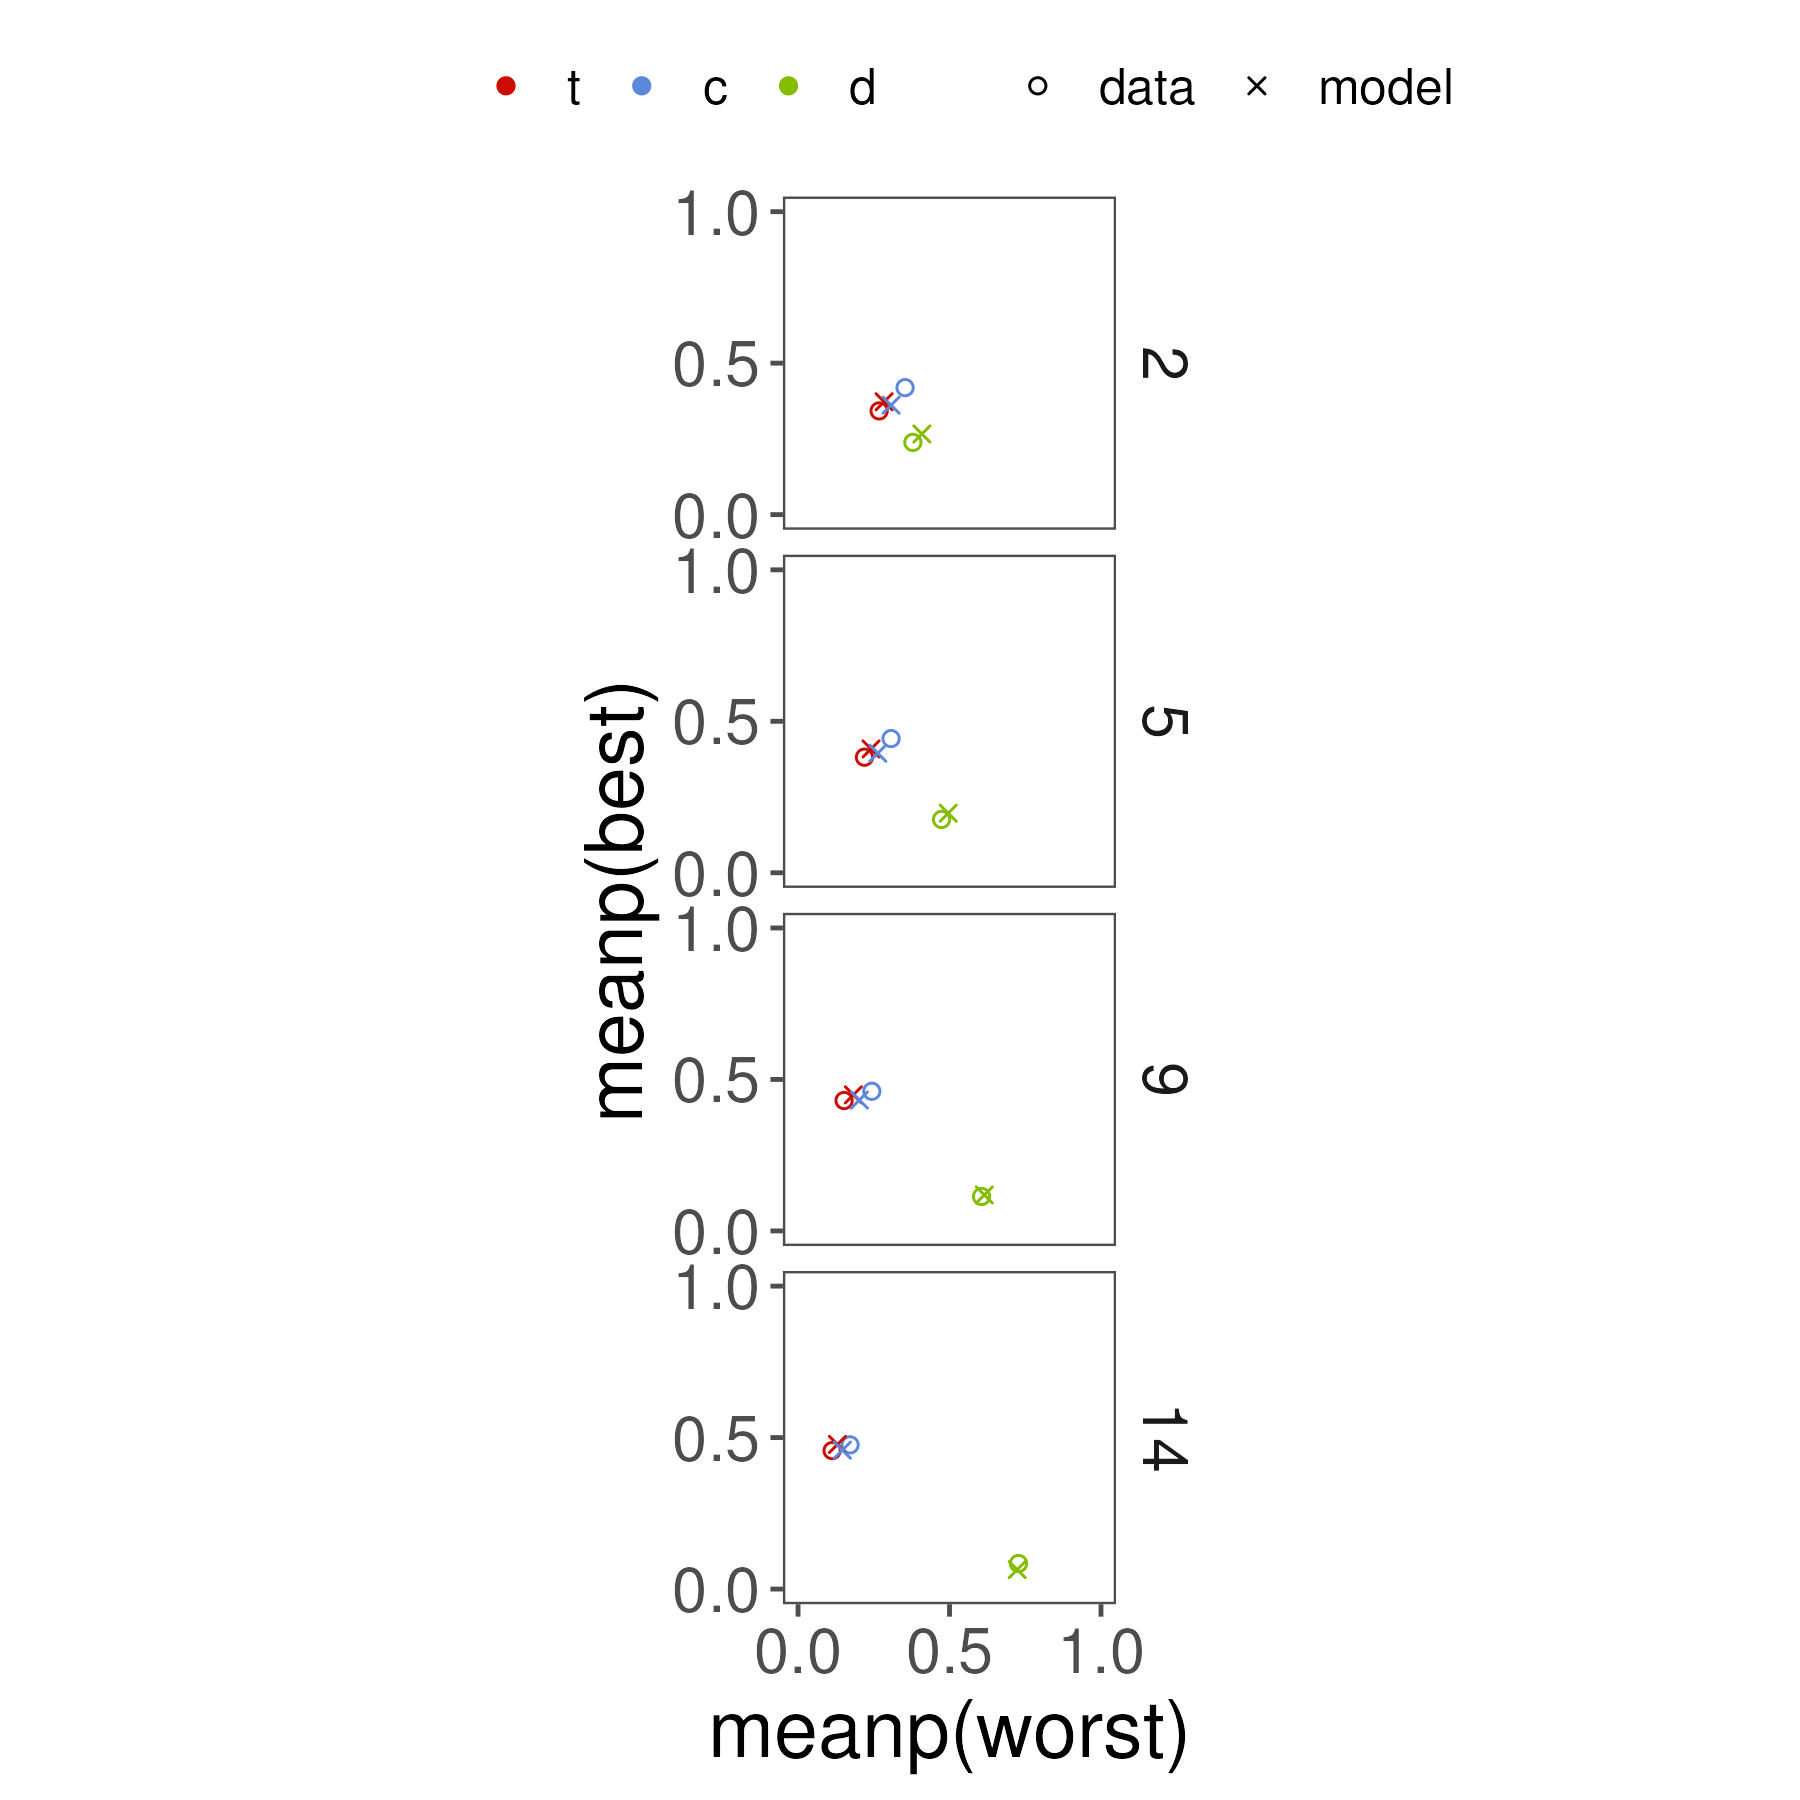
\includegraphics[width=\linewidth]{figures/maxdiff_1_means_model_v_data.jpeg}
   \caption{Experiment 3 maxdiff model predictions for the mean target, competitor, and decoy best-worst choice proportions.}
   \label{fig:maxdiff_collapsed_preds}
\end{figure}

\begin{figure}
   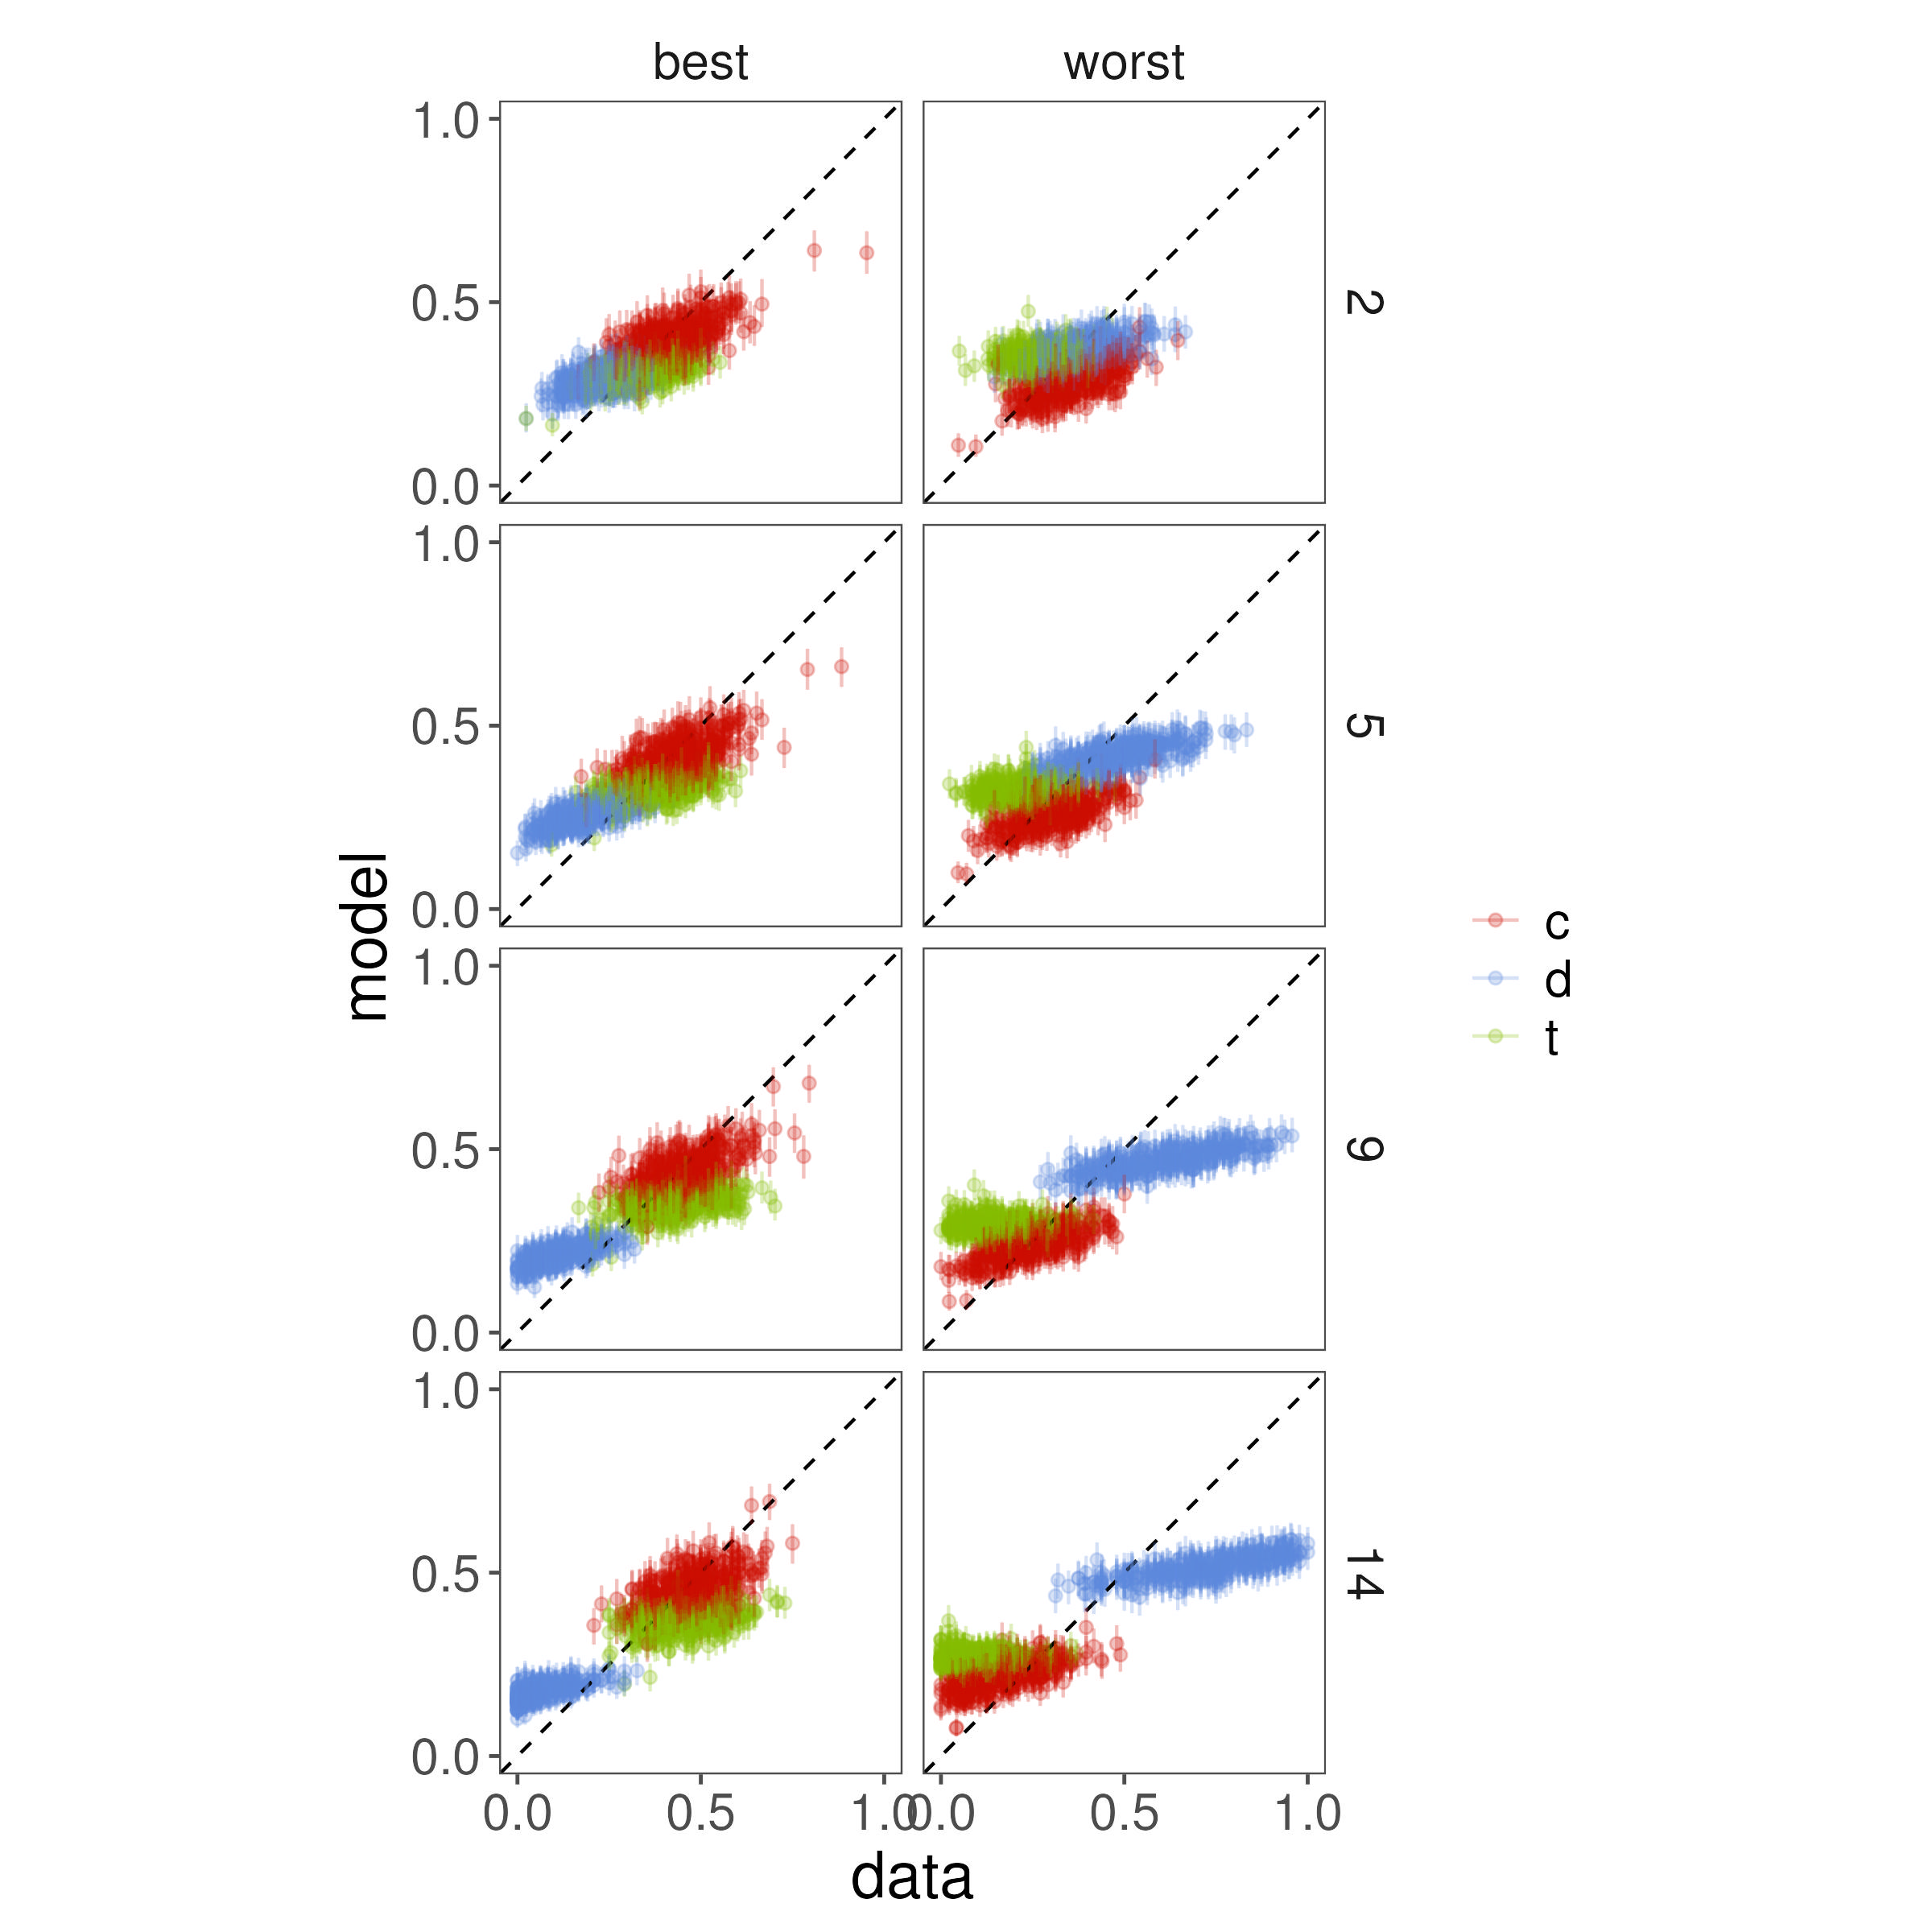
\includegraphics[width=\linewidth]{figures/maxdiff_1_subjectmeans_model_v_data.jpeg}
   \caption{Experiment 3 maxdiff model predictions for the mean target, competitor, and decoy best-worst participant-level choice proportions, conditioned on TDD (rows) and choice type, i.e. best v. worst (columns). Vertical error bars are $95\%$ HDIs.}
   \label{fig:maxdiff_sub_preds}
\end{figure}

\section{Discussion}
In Experiment 3, I showed that, in support of the Thurstonian perceptual choice model introduced in Chapter 2, correlated valuations can induce dissociations in best-worst choices. Specifically, given a target, competitor, and decoy option (borrowing the terminology of the attraction effect), the competitor is more likely than the target to be selected as best ($B(C)>B(T)$), but the competitor is also more likely than the target to be selected as worst ($W(C)>W(T)$). This prediction was made using the perceptual choice model of Chapter 2, conditioned on the parameters estimated from Experiment 3. Furthermore, the prediction was made with different set of participants and a completely different experimental task. This level of predictive success is atypical in psychology and even relatively uncommon in the cognitive modeling literature. 

The maxdiff model, the most common analysis technique for best-worst choice \parencite{marleyProbabilisticModelsBest2005,hawkinsIntegratingCognitiveProcess2014a,muhlbacher2016experimental,de2017relations}, cannot accomodate these results.  

The maxdiff model assumes that, when selecting the best and worst option, the decision-maker picks the option with the highest and lowest utility, respectively. The utilities of each option are independently distributed, and the decision-maker uses the same utility for both best and worst choices. The use of a single utility scale is to some extent a convenience assumption. \textcite{marleyProbabilisticModelsBest2005} explored several theoretical models, including the case where best and worst utilities exist on independent ratio scales, though such a model does not seem to have been adopted by substantive researchers. \textcite{marleyProbabilisticModelsSetdependent2008} demonstrated set-dependent best-worst choice models, which allows for different context dependence based on choice sets, albeit with best and worst choices still a function on a common underlying utility scale. 

\textcite{hawkins2019like} also argued that best and worst choices rely on a common utility representation. They fit the maxdiff model to 5 best-worst datasets and showed, via Bayesian mixture modeling, that the overwhelming majority of participants were best fit by a model with a single utility representation. 

\textcite{gervzinivc2021estimating} argued (and provided evidence for) the claim that while best and worst choices rely on a common utility scale, people use two distinct decision rules for best choices and worst choices. They argued that the former is compensatory (i.e., allowing tradeoffs between attributes), while the latter is non-compensatory (i.e., disallowing tradeoffs to minimize future regret). 

The Thurstonian perceptual model, used for the current predictions, also employs a common utility scale for both best and worst choices. However, the model does not assume independently distributed utilities, as assumed by the maxdiff model \parencite{de2017relations}. Thus, the claims of \textcite{hawkinsBestTimesWorst2014} and \textcite{hawkins2019like} are not necessarily falsified; rather, they are amended to account for correlations between option utilities.

Due to the small effect size, I required a large amount of data to estimate these dissociations. Most best-worst choice research is applied (for example in transportation and healthcare economics), where researchers do not typically have access a large amount of participant-level data. Thus, researchers are unlikely to observe the dissociations in best-worst choice and will analyze the data using the maxdiff model. They may then arrive at incorrect conclusions regarding participants' preferences. 

% In a related paradigm, researchers have shown that allowing participants to reject all options from a set can affect choice. \textcite{tverskyChoiceConflictDynamics1992a} showed that people are more likely to reject all options if the options trade off on attributes compared to if one dominates the other. Other researchers have demonstrated that forced choice and free choice (when rejection is possible) can create markedly different choice patterns \parencite{dhar1997consumer,dhar1997context,dhar1996effect,dharEffectForcedChoice2003b,noguchiDescriptionexperienceGapChoice2016a,brazellNochoiceOptionDual2006b,parker2011rejectable,chernevChoiceOverloadConceptual2015}. 

I did not fit the Thurstonian perceptual model to Experiment 3. In Experiment 2, I asked participants estimate the size of the stimuli and used these direct size ratings to estimate the model parameters. It also seems unreasonable to expect researchers to fit a multivariate Thurstonian model to most best-worst choice studies, given limitations in data and potential issues with parameter identifiability. 

The central purpose for conducting best-worst choice studies is to identify participants' preference distributions on a set of options. Best-worst choice is less cognitively demanding on participants than asking them to rank all options and far more efficient than pairwise forced choices on all combinations of options \parencite{louviere2008modeling}. In many cases, analyzing best-worst data with the maxdiff model may be the best approach, especially if researchers have no reason to believe that options are strongly correlated. It is an open question, left for future research, whether correlations between options in applied choice research can create similar dissociations in best-worst choice. 

The current study only considered Case 3 best-worst choice \parencite{marleyModelsBestWorst2012}, where the attributes of options (in our case, height/width, TDD, diagonal) are systematically manipulated to examine their impact on preferences. I ignored Case 1 best-worst choice, where researchers are interested in preference for each option as a whole (e.g., a consumer's preference for cars over bicycles) or Case 2 best-worst choice, where researchers ask participants to select their preferred attribute from a set (e.g., a consumer's preference for short waiting times over easily accessible WiFi in a clinic). Future research should consider ways to generalize the current paradigm and results to the other best-worst choice types.

For the time being, I have identified a discrepancy between theory and data, in a prominent area of decision-making research. This gap is both theoretically and practically interesting. It is up to future researchers, myself included, to continue theoretical development in this line of study. 

\chapter{Valuations and Correlations in Preferential Choice}
\label{chapter_4}
\section{Introduction}
Thus far, the dissertation has focused on perceptual choice. This allowed me to reconcile conflicting findings from other researchers \parencite{spektorWhenGoodLooks2018b,trueblood2013not}. It also allowed me to develop a choice model from the ground up in a simplified choice environment. 

However, many decision theorists, in particular those who study context effects, are interested in a wide variety of choice environments. For example, the original demonstration of the attraction effect came from the marketing literature \parencite{huberAddingAsymmetricallyDominated1982d}, where participants selected amongst hypothetical consumer products. In this chapter, I generalize the paradigm and model from Chapter 2 to consumer choice. Below, I demonstrate results similar to Chapter 2.

\subsection{Expanding the Paradigm to Preferential Choice}

In Experiment 2, I collected psychophysical ratings and used those to estimate the parameters of a Thurstonian choice model, which I then applied to make predictions for choices in the same experiment. To test this approach in preferential choice, it was necessary to collect continuous preference ratings from participants. In Experiment 4, I collected both pricing data (the best continuous measure for consumer stimuli) and choices.

In most studies of consumer preference, researchers collect choice data rather than ratings. There are good reasons for this. The literature on willingness to pay (WTP; the largest amount a given consumer would be willing to pay for a particular product) has shown that, when responding to hypothetical survey questions, participants tend to over-estimate their WTP by a sizeable aomunt \parencite{breidertREVIEWMETHODSMEASURING2006,schmidtAccuratelyMeasuringWillingness2020}, \parencite[c.f.~]{miller2011should}. It is generally more advisable to collect discrete choices, rather than ordinal or continuous ratings, when attempting to measure preferences.

These concerns, while crucial to applied researchers, are not relevant to the current study, as I am interested in participants' relative rather than absolute ratings. In other words, if participants over (or under) estimate their preferences by a constant, but generally rate higher valued options more highly than lower valued options, I can obtain reliable estimates of the $\rho$ parameters. As in Experiment 2, where I was concerned with whether participants' estimates of perceived size increased with absolute size (regardless of how it deviated from actual size), here I am interested in a measure that increases monotonically with the value participants place on each option. 

Other researchers have studied context effects with ratings measures. \textcite{wedellUsingJudgmentsUnderstand} collected Likert scale attractiveness ratings for attraction effect stimuli, generally finding that the presence of a decoy increased mean ratings for a target option. \textcite{windschitl2004dud} asked participants to judge the likelihood of various events (also on a Likert scale). They found that the presence of a "dud" (highly unlikely) alternative increased participants' ratings of focal options. \textcite{caiWhenAlternativeHypotheses2023} and \textcite{fang2024context} demonstrated similar effects by collecting continuous probability judgments.

To my knowledge, however, there has been no research systematically connecting valuations and choices in a single experiment through application of a choice model. Thus, I collected ratings to estimate the multivariate normal parameters $\boldsymbol{\mu}$ and $\boldsymbol{\Sigma}$ for the choice model from Chapter 2 and used these to predict consumer choice data collected from the same group of participants.

\subsection{Correlations in Preferential Choice}
In Chapter 2, I showed that the model could capture the repulsion effect in perceptual choice \parencite{spektorWhenGoodLooks2018b} through target-decoy correlations, estimated via the parameter $\rho_{TD}$. I am now interested in whether 1) preferential choice options also exhibit these correlations and 2) the model can capture the repulsion effect in preferential choice. 

The literature on the repulsion effect in preferential choice is relatively sparse. \textcite{liaoInfluenceDistanceDecoy2021} varied TDD in preferential choice and found a U-shaped relationship between TDD and RST (Relative Share of the Target), with the attraction effect occuring at low and high TDD levels but the repulsion effect occuring at more intermediate TDD levels. 

\textcite{banerjeeFactorsThatPromote2024} demonstrated a binary-ternary form of the repulsion effect using the stimuli depicted in Figure~\ref{fig:banerjee_stim}, across multiple experiment. Participants saw either two or three options on each trial, each varying on two dimensions. The options were consumer choice products from a number of categories (e.g., cameras, coffee makers, laptops), and the dimension names varied by product category (e.g., coffee makers' dimensions were brew speed and features). Attribute values were always displayed numerically using ratings of 1-100.

In each set, the target was always the most extreme option - particularly high on one dimension and particularly low on the other dimension. The competitor was a more intermediate option. For example, consider the blue-colored stimuli in Figure~\ref{fig:banerjee_stim}. $t$ is very high on $X$ and very low on $Y$. Compared to $t$, $c$ is slightly worse on $X$ but slightly better on $Y$. $d$, however, is as high as $t$ on $X$ but even worse on $Y$. 

Using these stimuli and across multiple experiments, \textcite{banerjeeFactorsThatPromote2024} showed that the competitor's choice share increased from binary to ternary choice sets, $P(C|[T,C,D])>P(C|[T,C])$, in violation of the regularity principle \parencite{marley1989random}. In other experiments, they also showed that the repulsion effect decreased with $TDD$.

\begin{figure}
    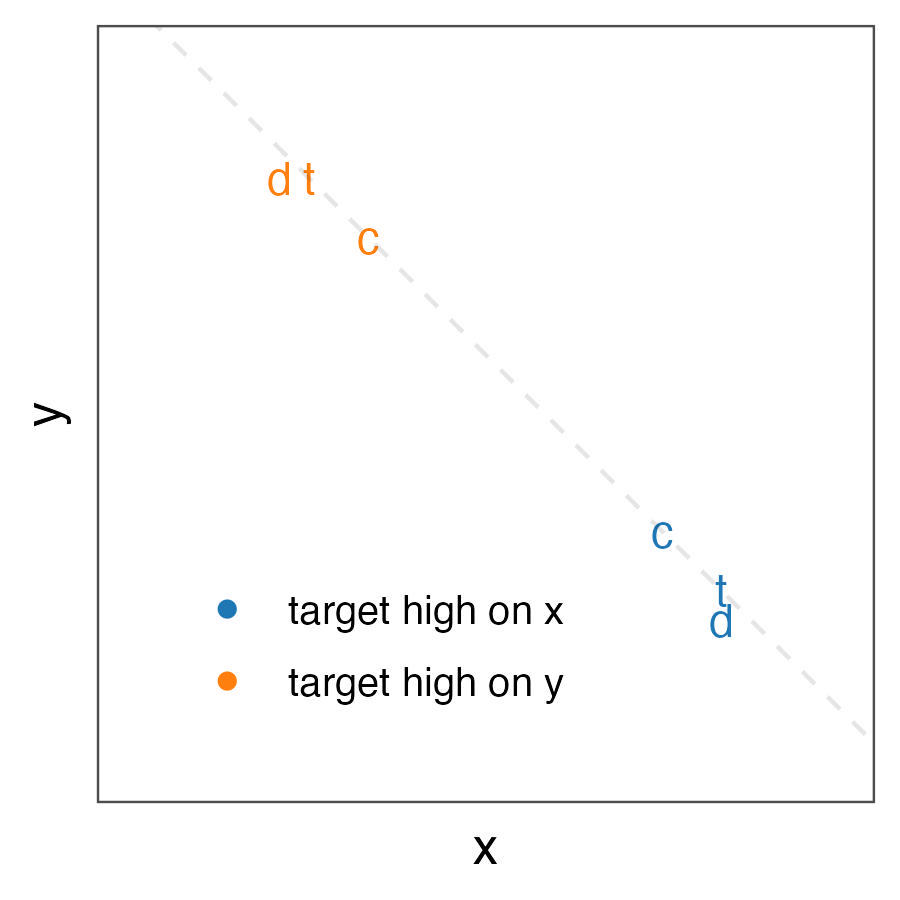
\includegraphics[width=100mm]{figures/banerjee_stim.jpeg}
    \caption{Graphical depiction of a subset of the stimuli used in \textcite{banerjeeFactorsThatPromote2024}, Experiment 5. Target, competitor, and decoy are labeled \textit{t}, \textit{c}, and \textit{d}, respectively. Dimensions are (generically) labeled X and Y.}. The choice sets vary based on whether the target is higher on the X or Y dimension.
    \label{fig:banerjee_stim}
\end{figure}

\textcite{banerjeeFactorsThatPromote2024}'s experiments compared binary to ternary choice rather than ternary to ternary choice, as in \textcite{spektorWhenGoodLooks2018b}. To do a ternary-ternary comparison, one would "flip" the target and competitor labels, such that the target is the intermediate option, the competitor is the extreme option, and the decoy is nearby the new, intermediate target. It is in one sense, quite interesting, that \textcite{banerjeeFactorsThatPromote2024} were able to generate violations of regularity in this binary to ternary comparison. However, the results are somewhat limited by the fact that the target was always more extreme than the competitor.

\textcite{banerjeeFactorsThatPromote2024} argued that their results are consistent with the "tainting hypothesis" \parencite{simonson2014vices} because the repulsion effect is strongest when the target and decoy are similar. They also argued that the decoy, may have caused participants to focus more attention on the competitor's superior dimension. For example, in the blue choice set of Figure~\ref{fig:banerjee_stim}, the decoy is quite poor on $Y$ while being equally good as the target on $X$, so participants may have focused more attention on $Y$, leading to a preference for the target. 

\textcite{banerjeeFactorsThatPromote2024}'s results are interesting and worth exploring further. The authors are also remarkably transparent about their stimulus generation procedure, in addition to posting their data online, so their stimuli were a perfect candidate for the Experiment 4.

\section{Experiment 4}

With Experiment 4, I sought to collect ratings and choice data in a preferential choice setting using (a subset of) \textcite{banerjeeFactorsThatPromote2024}'s Experiment 5 stimuli. I used these data to estimate the parameters of the choice model from Chapter 2. 

For a ratings measure, I asked participants to assign prices to each option. Though people often overestimate prices \parencite{breidertREVIEWMETHODSMEASURING2006}, pricing measures are approximately continuous and monotonic with value and are thus comparable to estimated area (the value measure from Experiment 2).

\subsection{Methods}

\subsubsection{Participants}
137 U.S. adults participated in the experiment. Participants were recruited from Prolific, an online platform for posting research studies, and they were paid $\$5$ for their participation. 24 participants were removed from all analyses for failing catch trials (see below), leaving a final sample size of $N=113$. The mean age was $38.89$ ($SD=11.48$). $61$ participants identified as female, $50$ identified as male, $1$ participant identified as non-binary, and $1$ participant preferred not to say.

\subsubsection{Stimuli}

The stimuli were borrowed from \textcite{banerjeeFactorsThatPromote2024}'s Experiment 1. The stimuli were hypothetical consumer choice products. All stimuli varied on two attributes, each of which ranged from 0-100. The products came from four different categories: televisions, washing machines, laptops, and microwave ovens. 

The attributes varied by category. Televisions varied on screen size and average lifespan. Washing machines varied on average lifespan and energy savings. Laptops varied on processing speed and memory (RAM). Microwave ovens varied on warranty and cooking power. 

Within each category, one attribute was arbitrarily designated as dimension 1 and another as dimension 2 (see below). 

\subsubsection{Design}

The experiment took place in two phases: pricing and choice. The trial types were identical for both phases.

In each phase, there were two types of trials: critical trials and catch trials. The critical trial stimuli are shown in Figure~\ref{fig:ce_rating_stim}. 

There were two types of critical trials: those designed to elicit the repulsion effect (a replication of \citeauthor{banerjeeFactorsThatPromote2024}), and those designed to elicit the attraction effect. Within both the attraction and repulsion trials, I varied which dimension the target was higher on (1 or 2), $TDD$ (designated near or far), and product category (microwaves, washing machines, laptops, and televisions). Note that to create the attraction trials, I simply "shifted" the target and competitor towards the center of the attribute space. That is, target and competitor are equally similar in both repulsion and attraction trials, but they are both more extreme in the repulsion trials.

\begin{figure}
    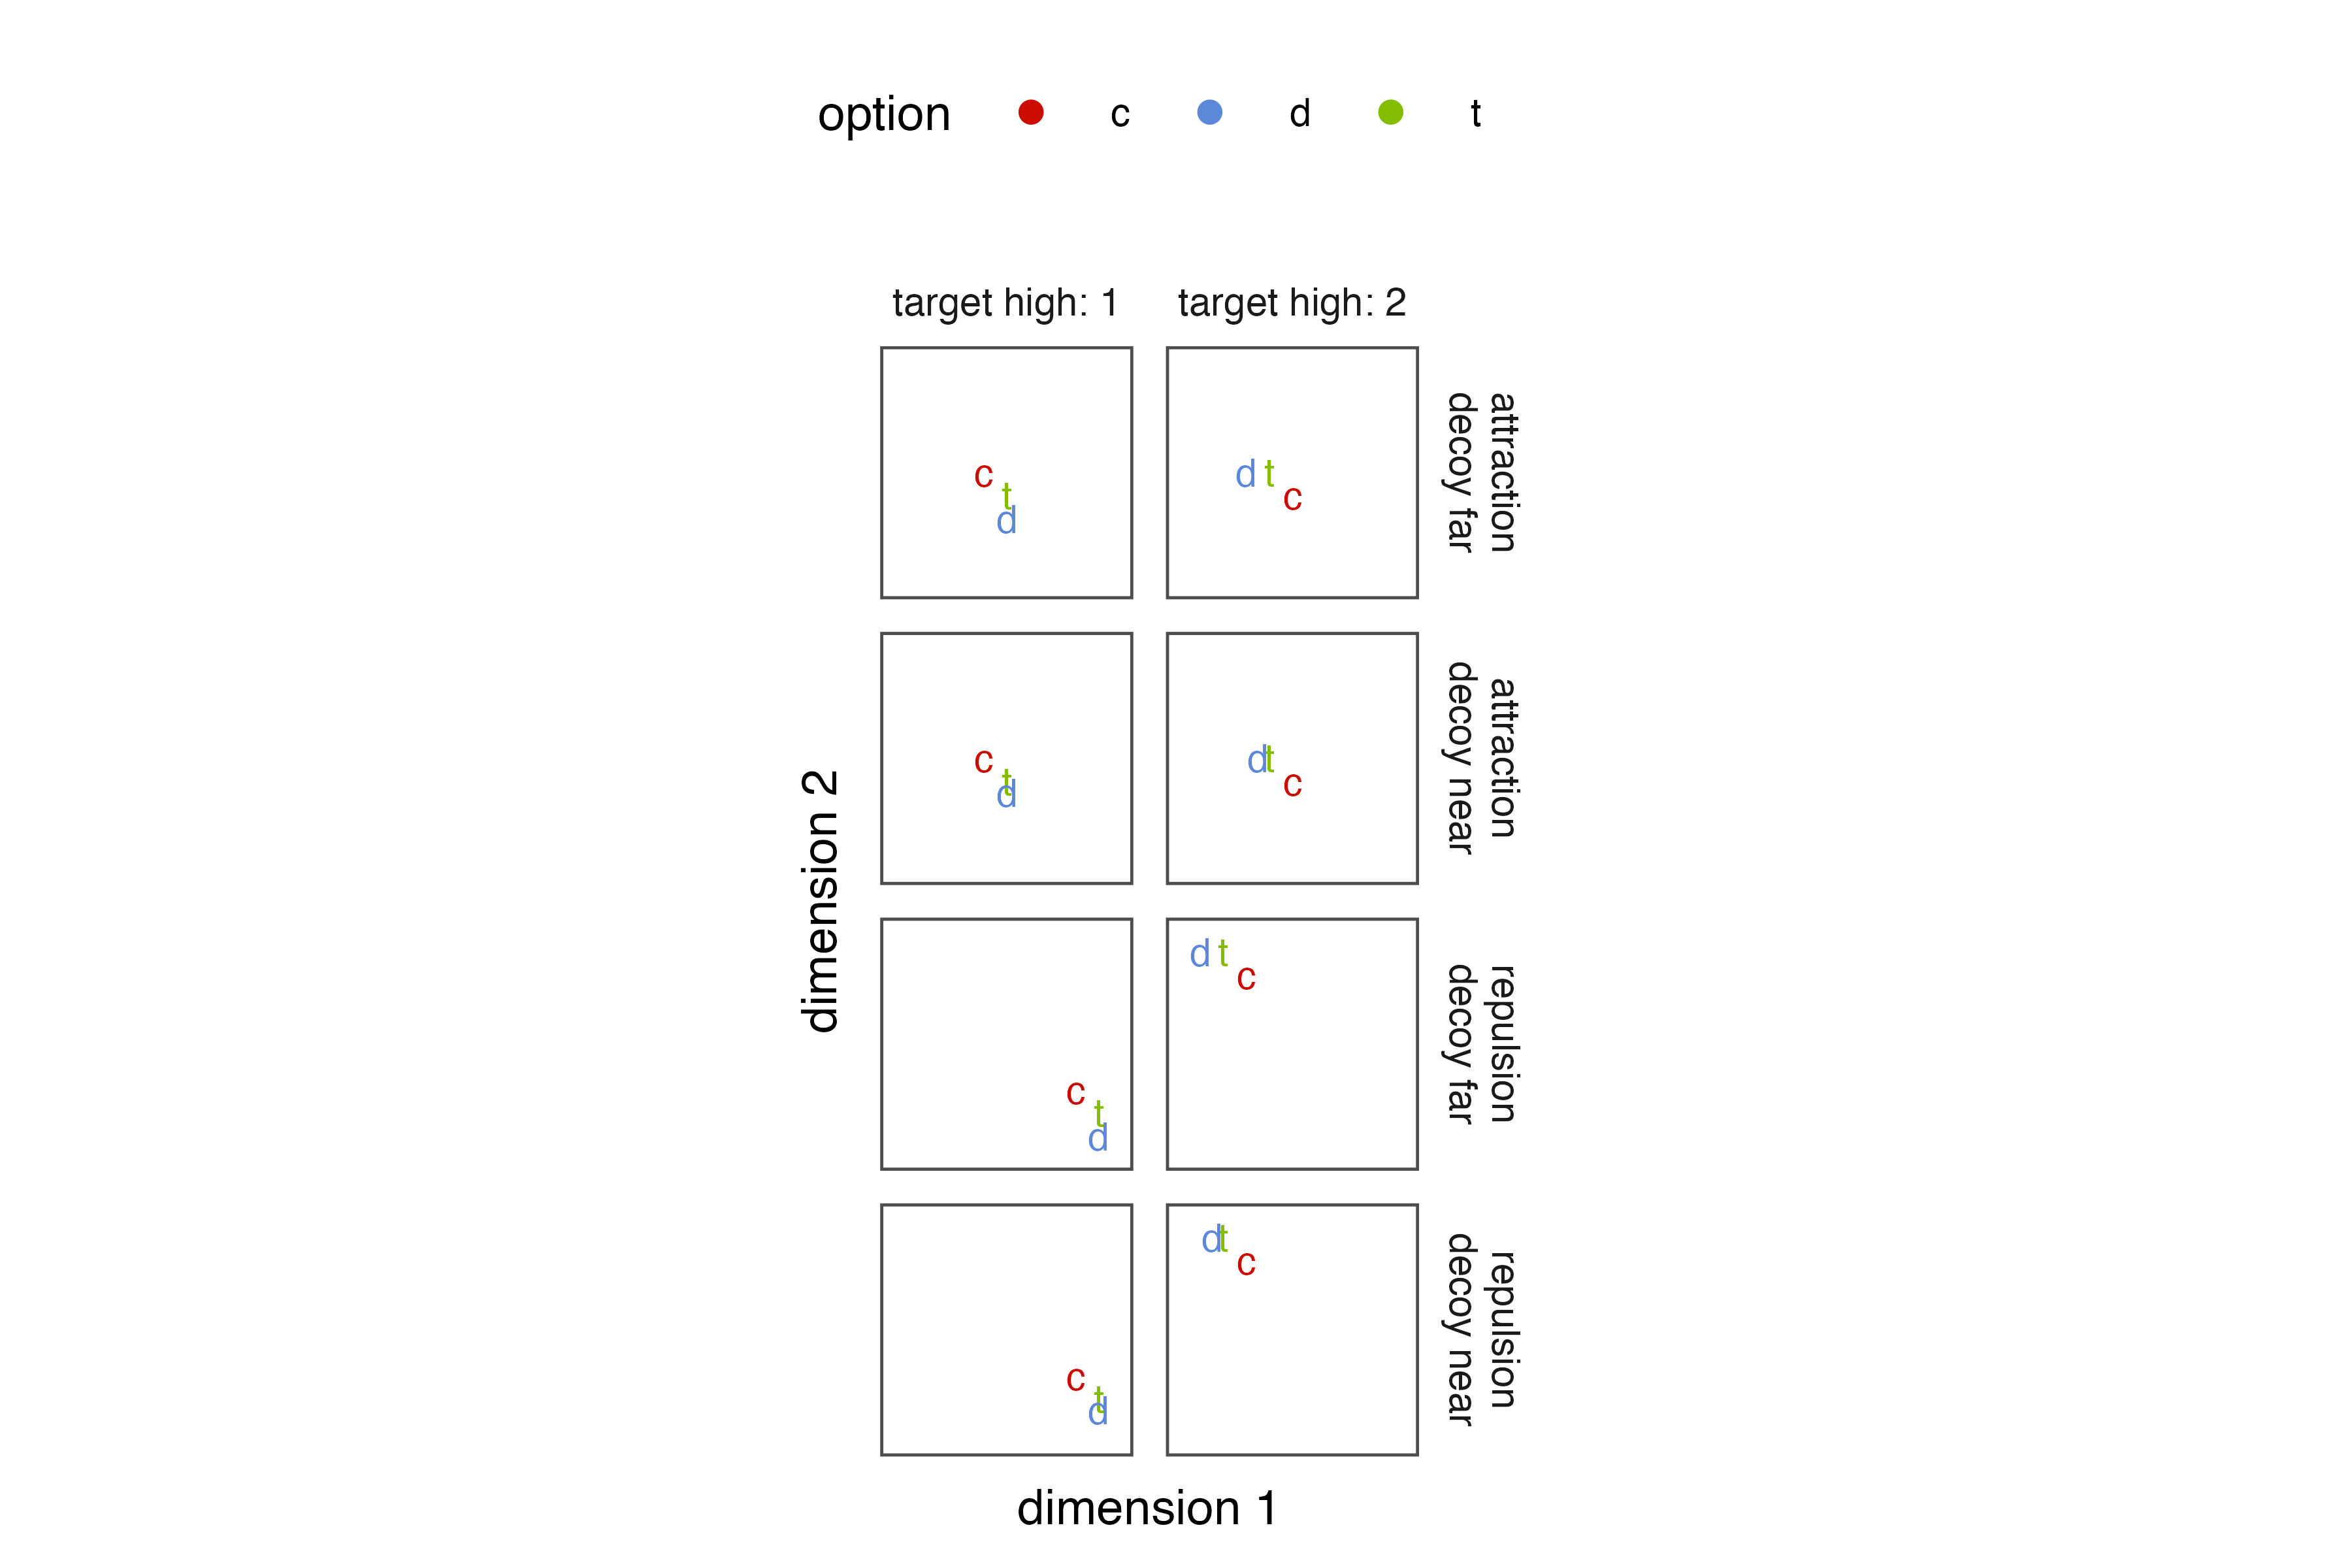
\includegraphics[width=150mm,scale=0.5]{figures/ce_rating_stim_for_paper.jpeg}
    \caption{Graphical depiction of the critical stimuli from Experiment 4. Rows show the different choice sets designed to elicit the attraction/repulsion effect, with the label also specifying whether the decoy is near or far from the target in attribute space. The columns indicate which dimension the target is high on (1 or 2).}
    \label{fig:ce_rating_stim}
\end{figure}

The catch trials were designed such that one option was clearly superior to the other two. On each catch trial, the superior option's dimension values were each randomly sampled from the distribution $U(50,95)$, while the two inferior option's dimension values were sampled from the distribution $U(5,50)$. All dimension values were rounded to multiples of 5. 

In each phase, there were 32 critical trials (16 designed to elicit the repulsion effect and 16 designed to elicit the attraction effect) and 8 catch trials.

I did not test binary repulsion effect trials, as in \textcite{banerjeeFactorsThatPromote2024}'s experiments, so I cannot assess the repulsion effect to the same degree as those authors. The goals here are, rather, to measure valuation correlations in consumer preference and attempt to relate them to choice.

\subsubsection{Procedure}

The experiment took place in two phases: a pricing phase and a choice phase.

Prior to the pricing phase, participants were provided with a cover story. According to the cover story, they were told to imagine that they run an online consumer goods resale business. On each trial, they would see three products, and they needed to determine which price to sell each product for. Participants were also told that they should determine a price that maximizes both profit and the likelihood the product is purchased. 

During the pricing trials, the three options were presented in a table, with the options in rows and the attributes in columns. All attributes were represented numerically. The options were labeled A, B, and C. The last column of the table contained three boxes, which participants used to type in their selling price for each option. Participants typed in their selling price, and then clicked a button on screen to move onto the next trial. Both option order and dimension order was randomized on each trial. See Figure~\ref{fig:ce_rating_choice_trial} (left panel) for an example trial. Participants were only allowed to enter in whole numbers (e.g., dollars not cents).

\begin{figure}
    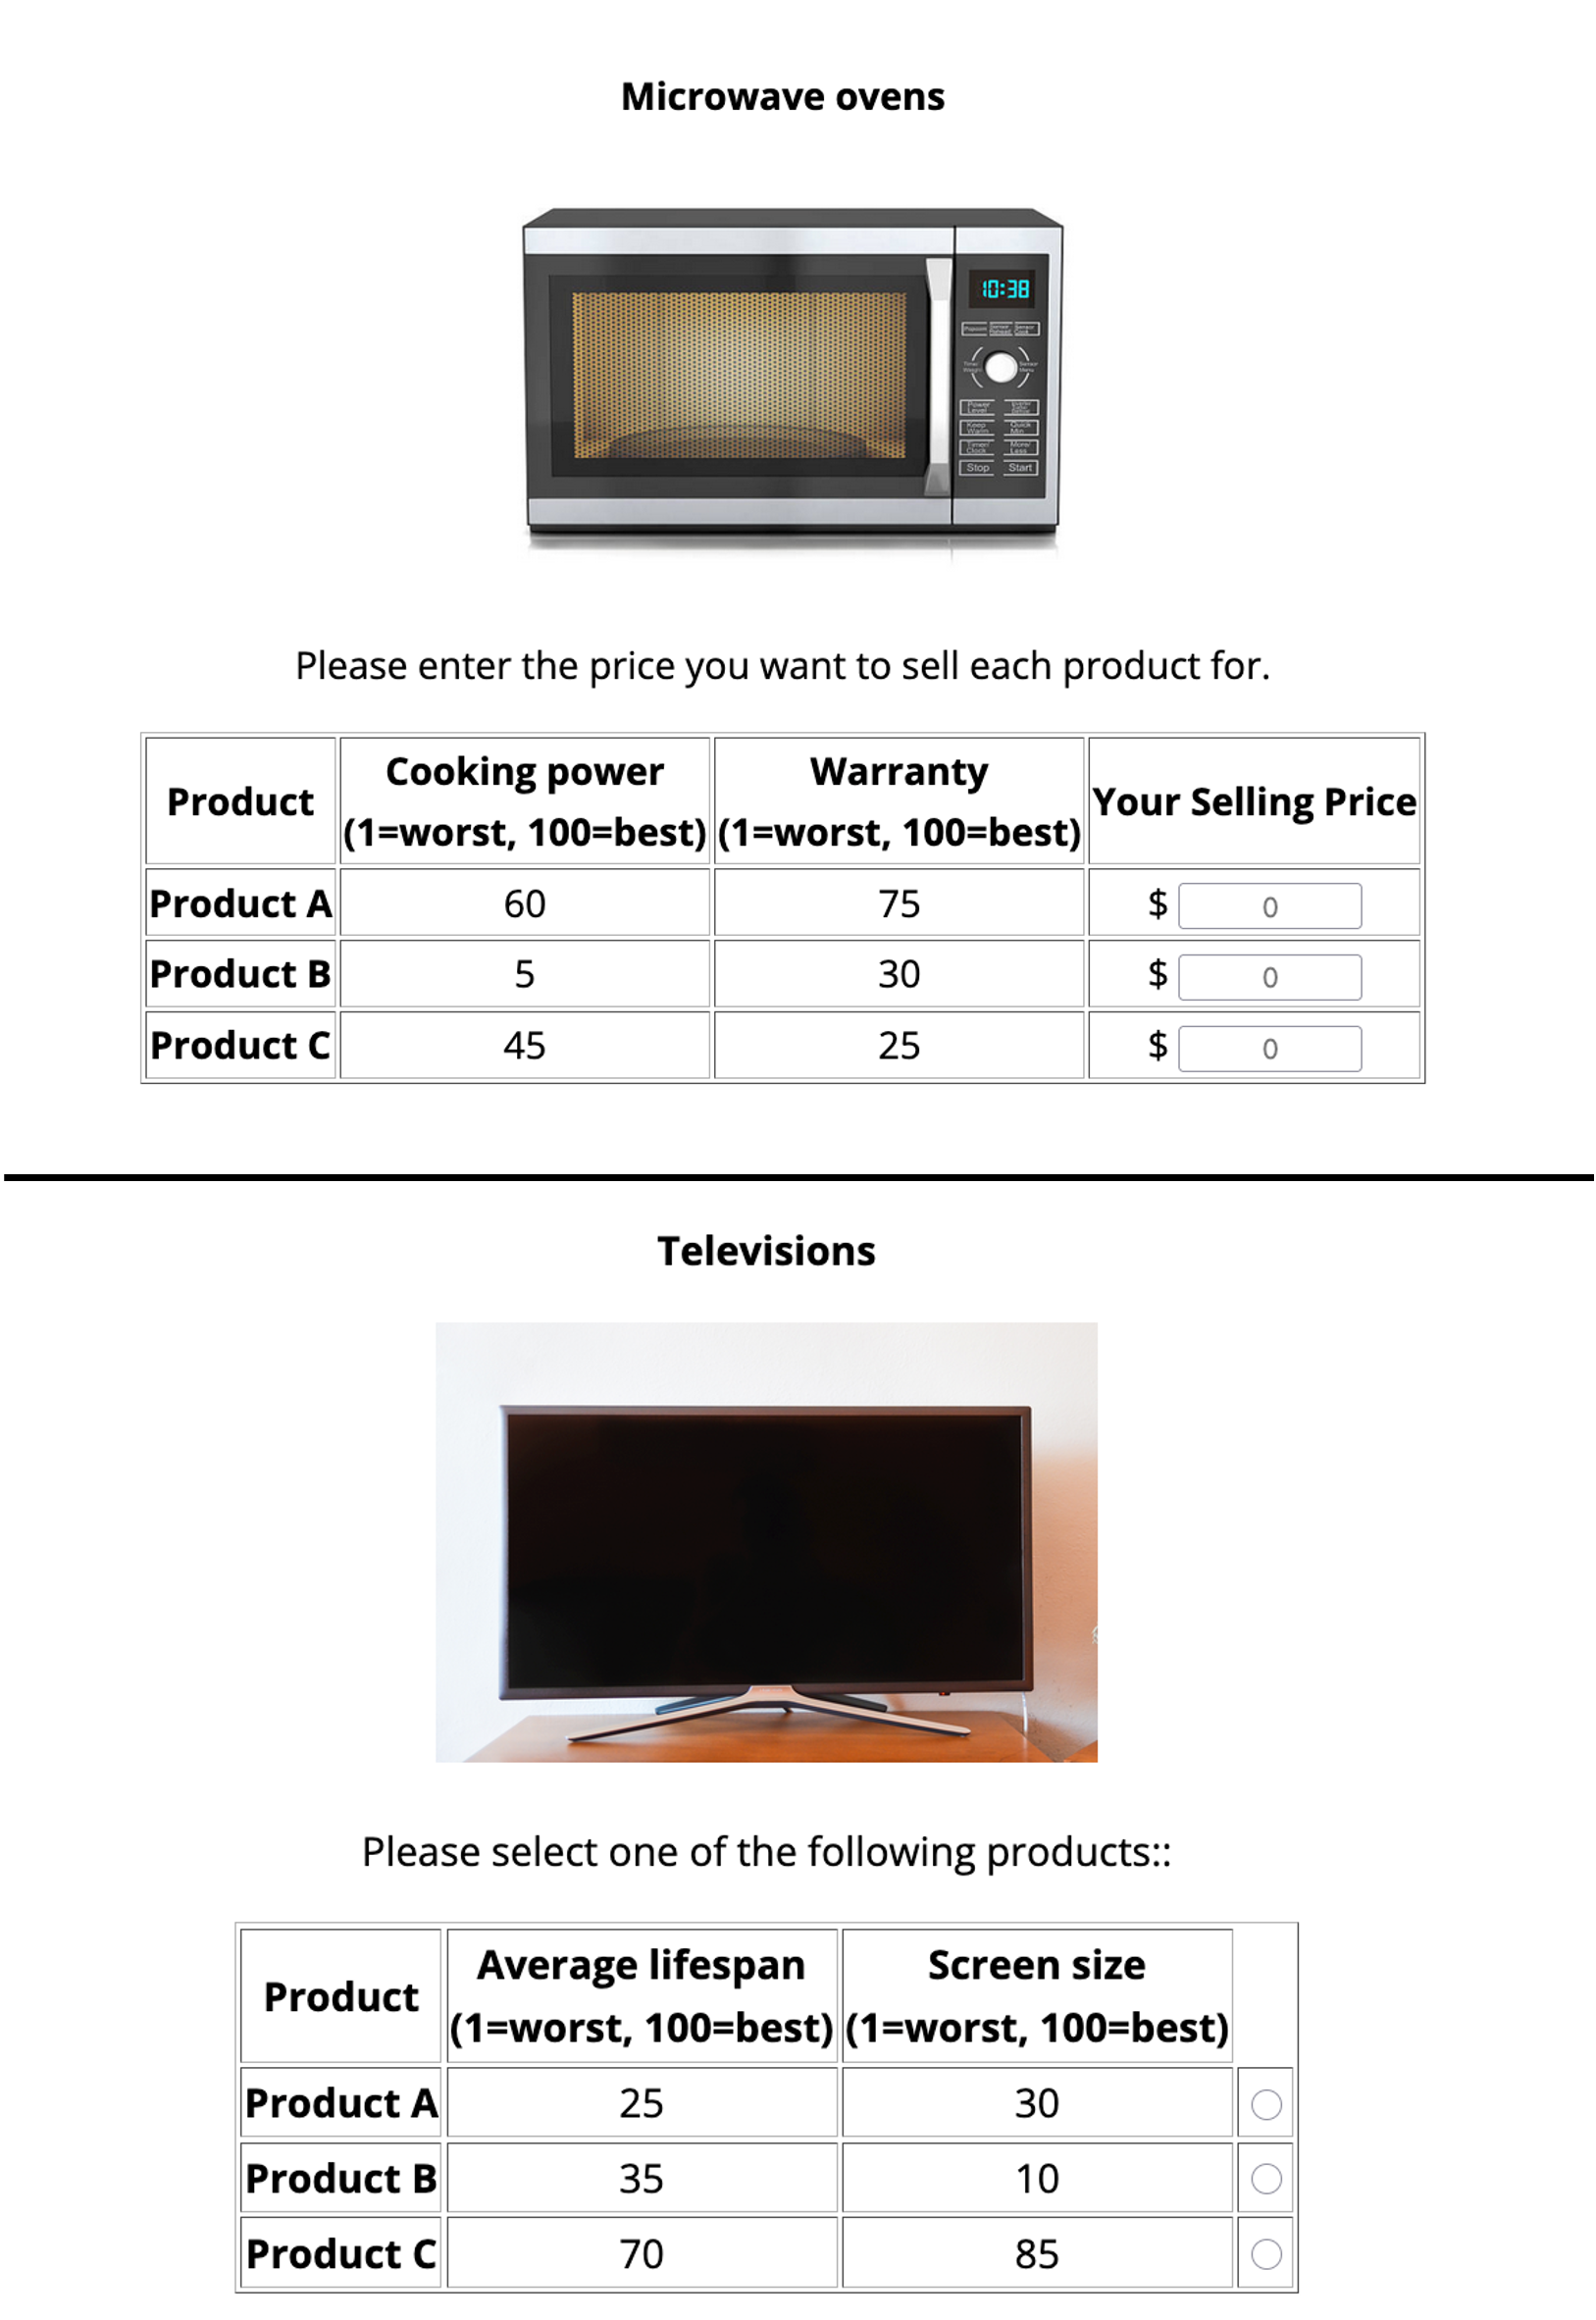
\includegraphics{figures/ce_rating_choice_example_trial.jpg}
    \caption{Sample trials from the pricing phase (top) and choice phase (bottom) in Experiment 4.}
    \label{fig:ce_rating_choice_trial}
\end{figure}

After completing all pricing trials, participants moved onto the choice phase. Prior to this phase, participants were told to imagine that they were purchasing consumer goods in bulk. On each trial, they were to select the option they wanted to purchase. 

As in the pricing phase, options were presented in a table, where option order and dimension order was randomized. See Figure~\ref{fig:ce_rating_choice_trial} (bottom) for an example trial.

After the choice phase, participants completed a short demographics form.

\subsection{Results}

\subsubsection{Data Processing}

First, I removed 24 participants who did not pass at least $5/8$ catch trials in both the pricing phase and the choice phase. To pass a pricing catch trial, the participant needed to price the superior option at least as high as the other two, inferior options. To pass a choice catch trial, the participant needed to select the superior option. 

\subsubsection{Pricing Trials}

First, I computed mean prices for the target, competitor, and decoy option within each trial type and product category. These means are shown in Figure~\ref{fig:price_m_by_effect_category}.

On average, participants priced the target and competitor higher than the decoy. They also assigned higher prices to products that are typically more expensive (e.g., washing machines are more expensive than microwave ovens). This suggests that participants were engaged with the task and, in a relative sense, performed the task well.

\begin{figure}
    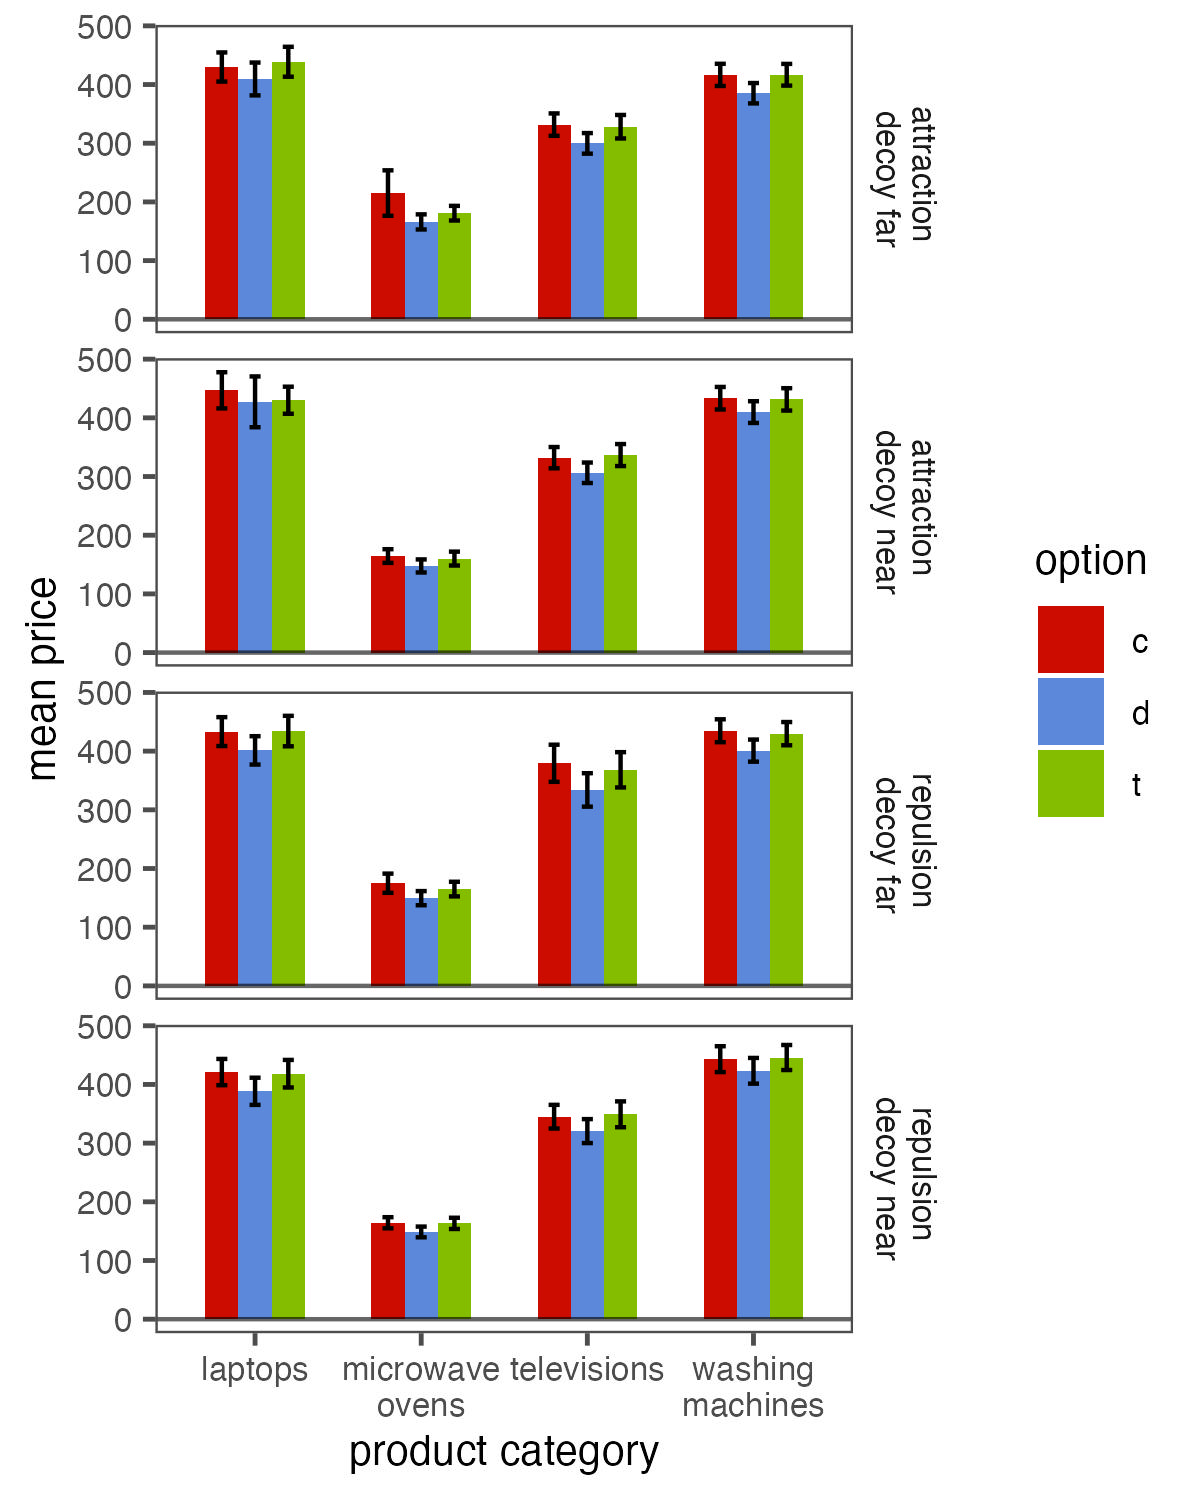
\includegraphics[width=200mm,scale=0.5]{figures/price_m_by_effect_category.jpeg}
    \caption{Experiment 4 mean prices by product category, option, and trial type. Error bars are $\pm 1\;\text{SEM}$.}
    \label{fig:price_m_by_effect_category}
\end{figure}

I performed a Bayesian modeling analysis comparable to that of Experiment 2. I estimated the mean prices and the correlations between prices. These results can be found in the Appendix. Below, I discuss descriptive statistics, but whenever I claim that one parameter value is greater than another, the reader can see the Appendix to support these conclusions. The ordering of these correlations, however, is the same in both the model-based and the descriptive analysis.

% Additionally, I report the descriptive values for all correlations, rather than those based on model estimates, as the latter as biased downard due to limited data \parencite{stephens2020state,merkle2023opaque}. 
To account for participant-level differences in pricing, I first z-scored all prices within each participant. To avoid the influence of outliers on correlation estimates, I removed trials in which at least one z-score had an absolute value $>3$. 

I computed the mean prices for target, competitor, and decoy options within each trial type, collapsing over product category and TDD, in Figure~\ref{fig:price_mu_model_data}. In both repulsion and attraction effect trials, the target and competitor do not differ in mean price, while both are priced higher than the decoy option.

\begin{figure}
    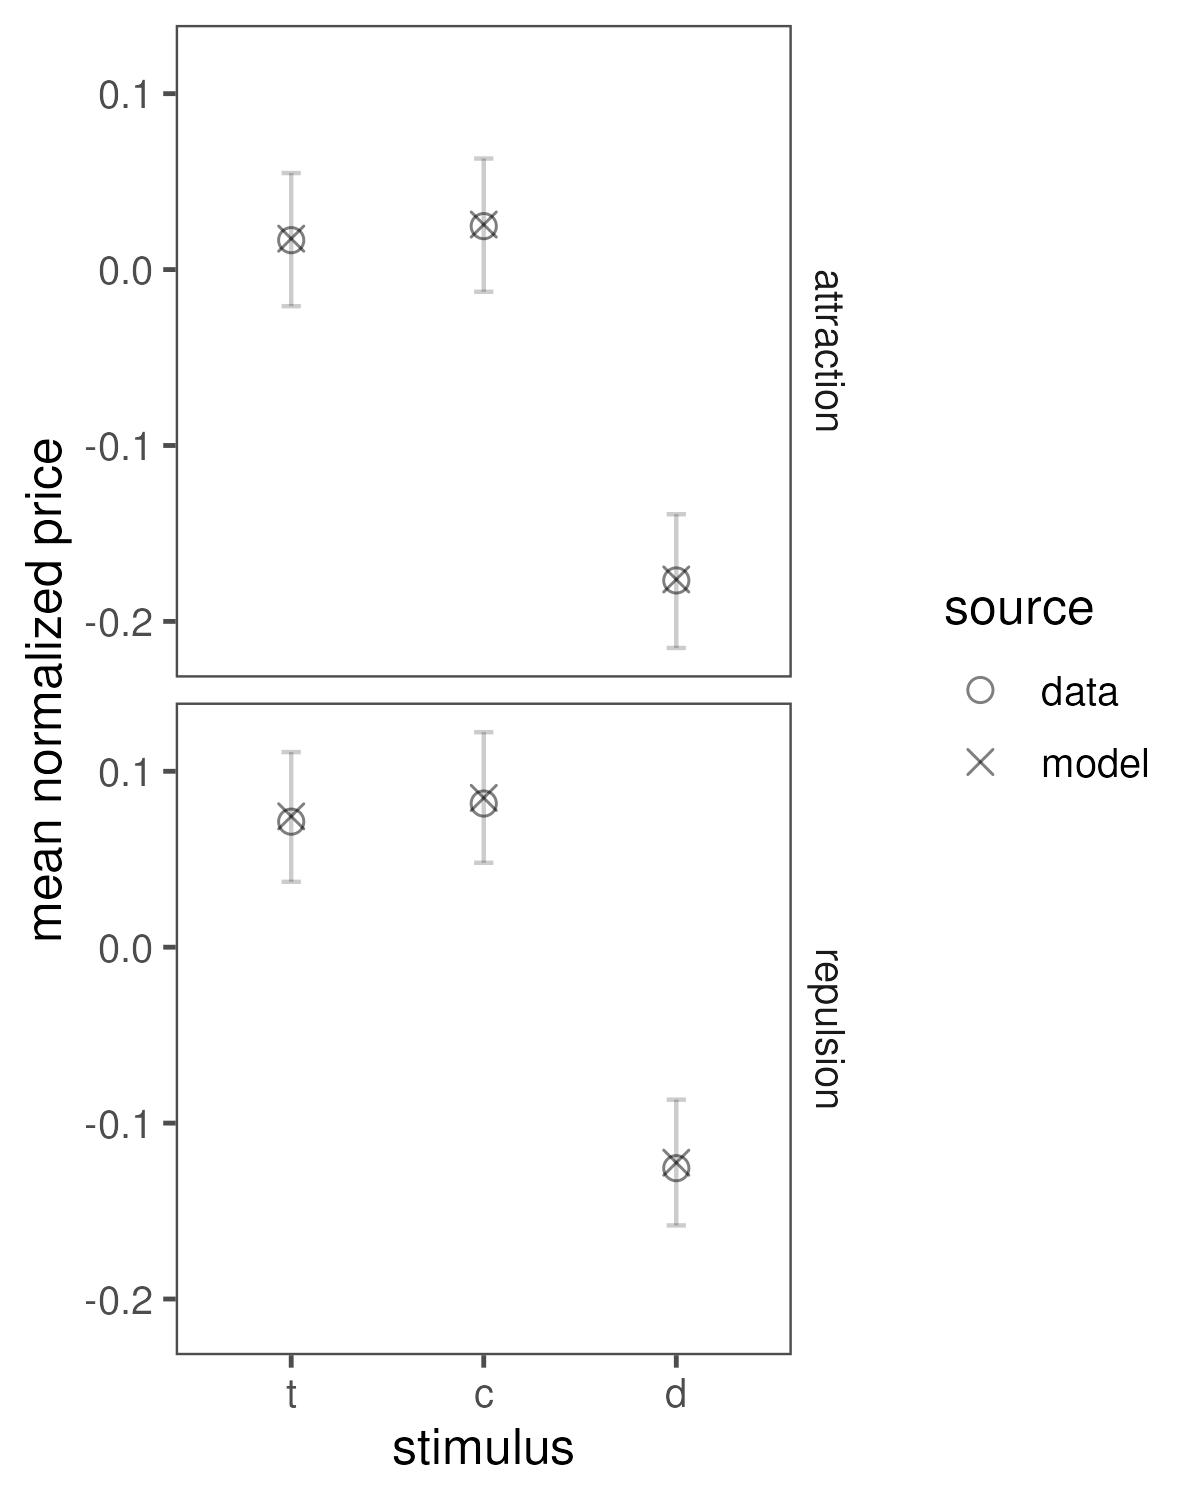
\includegraphics[scale=0.5, width=100mm]{figures/pricing_mu_model_data.jpeg}
    \caption{Experiment 4 mean prices for target, competitor, and decoy options in both repulsion and attraction trials. Model values are the means from the posterior distribution, and error bars are $95\%$ HDIs.}
    \label{fig:price_mu_model_data}
\end{figure}

I then computed correlations between the prices assigned to options within each trial type. I plot the z-scored prices in a series of scatterplots, with the Pearson correlations included. See Figure~\ref{fig:price_z_corplot_repulsion} for repulsion effect correlations and Figure~\ref{fig:price_z_corplot_attraction} for attraction effect correlations. 

In the repulsion trials, I replicated the results of Experiment 2, in that $\rho_{TD}>\rho_{TC}$ and $\rho_{TD}>\rho_{CD}$. Interestingly, I also found that $\rho_{TC}>\rho_{CD}$, while in Experiment 2 $\rho_{TC}\approx\rho_{CD}$.

In the attraction trials, I found that $\rho_{TC}\approx\rho_{TD}>\rho_{CD}$. In other words, the target and competitor are approximately equally similar as target and decoy, which are in turn more similar than competitor and decoy. 

\begin{figure}
    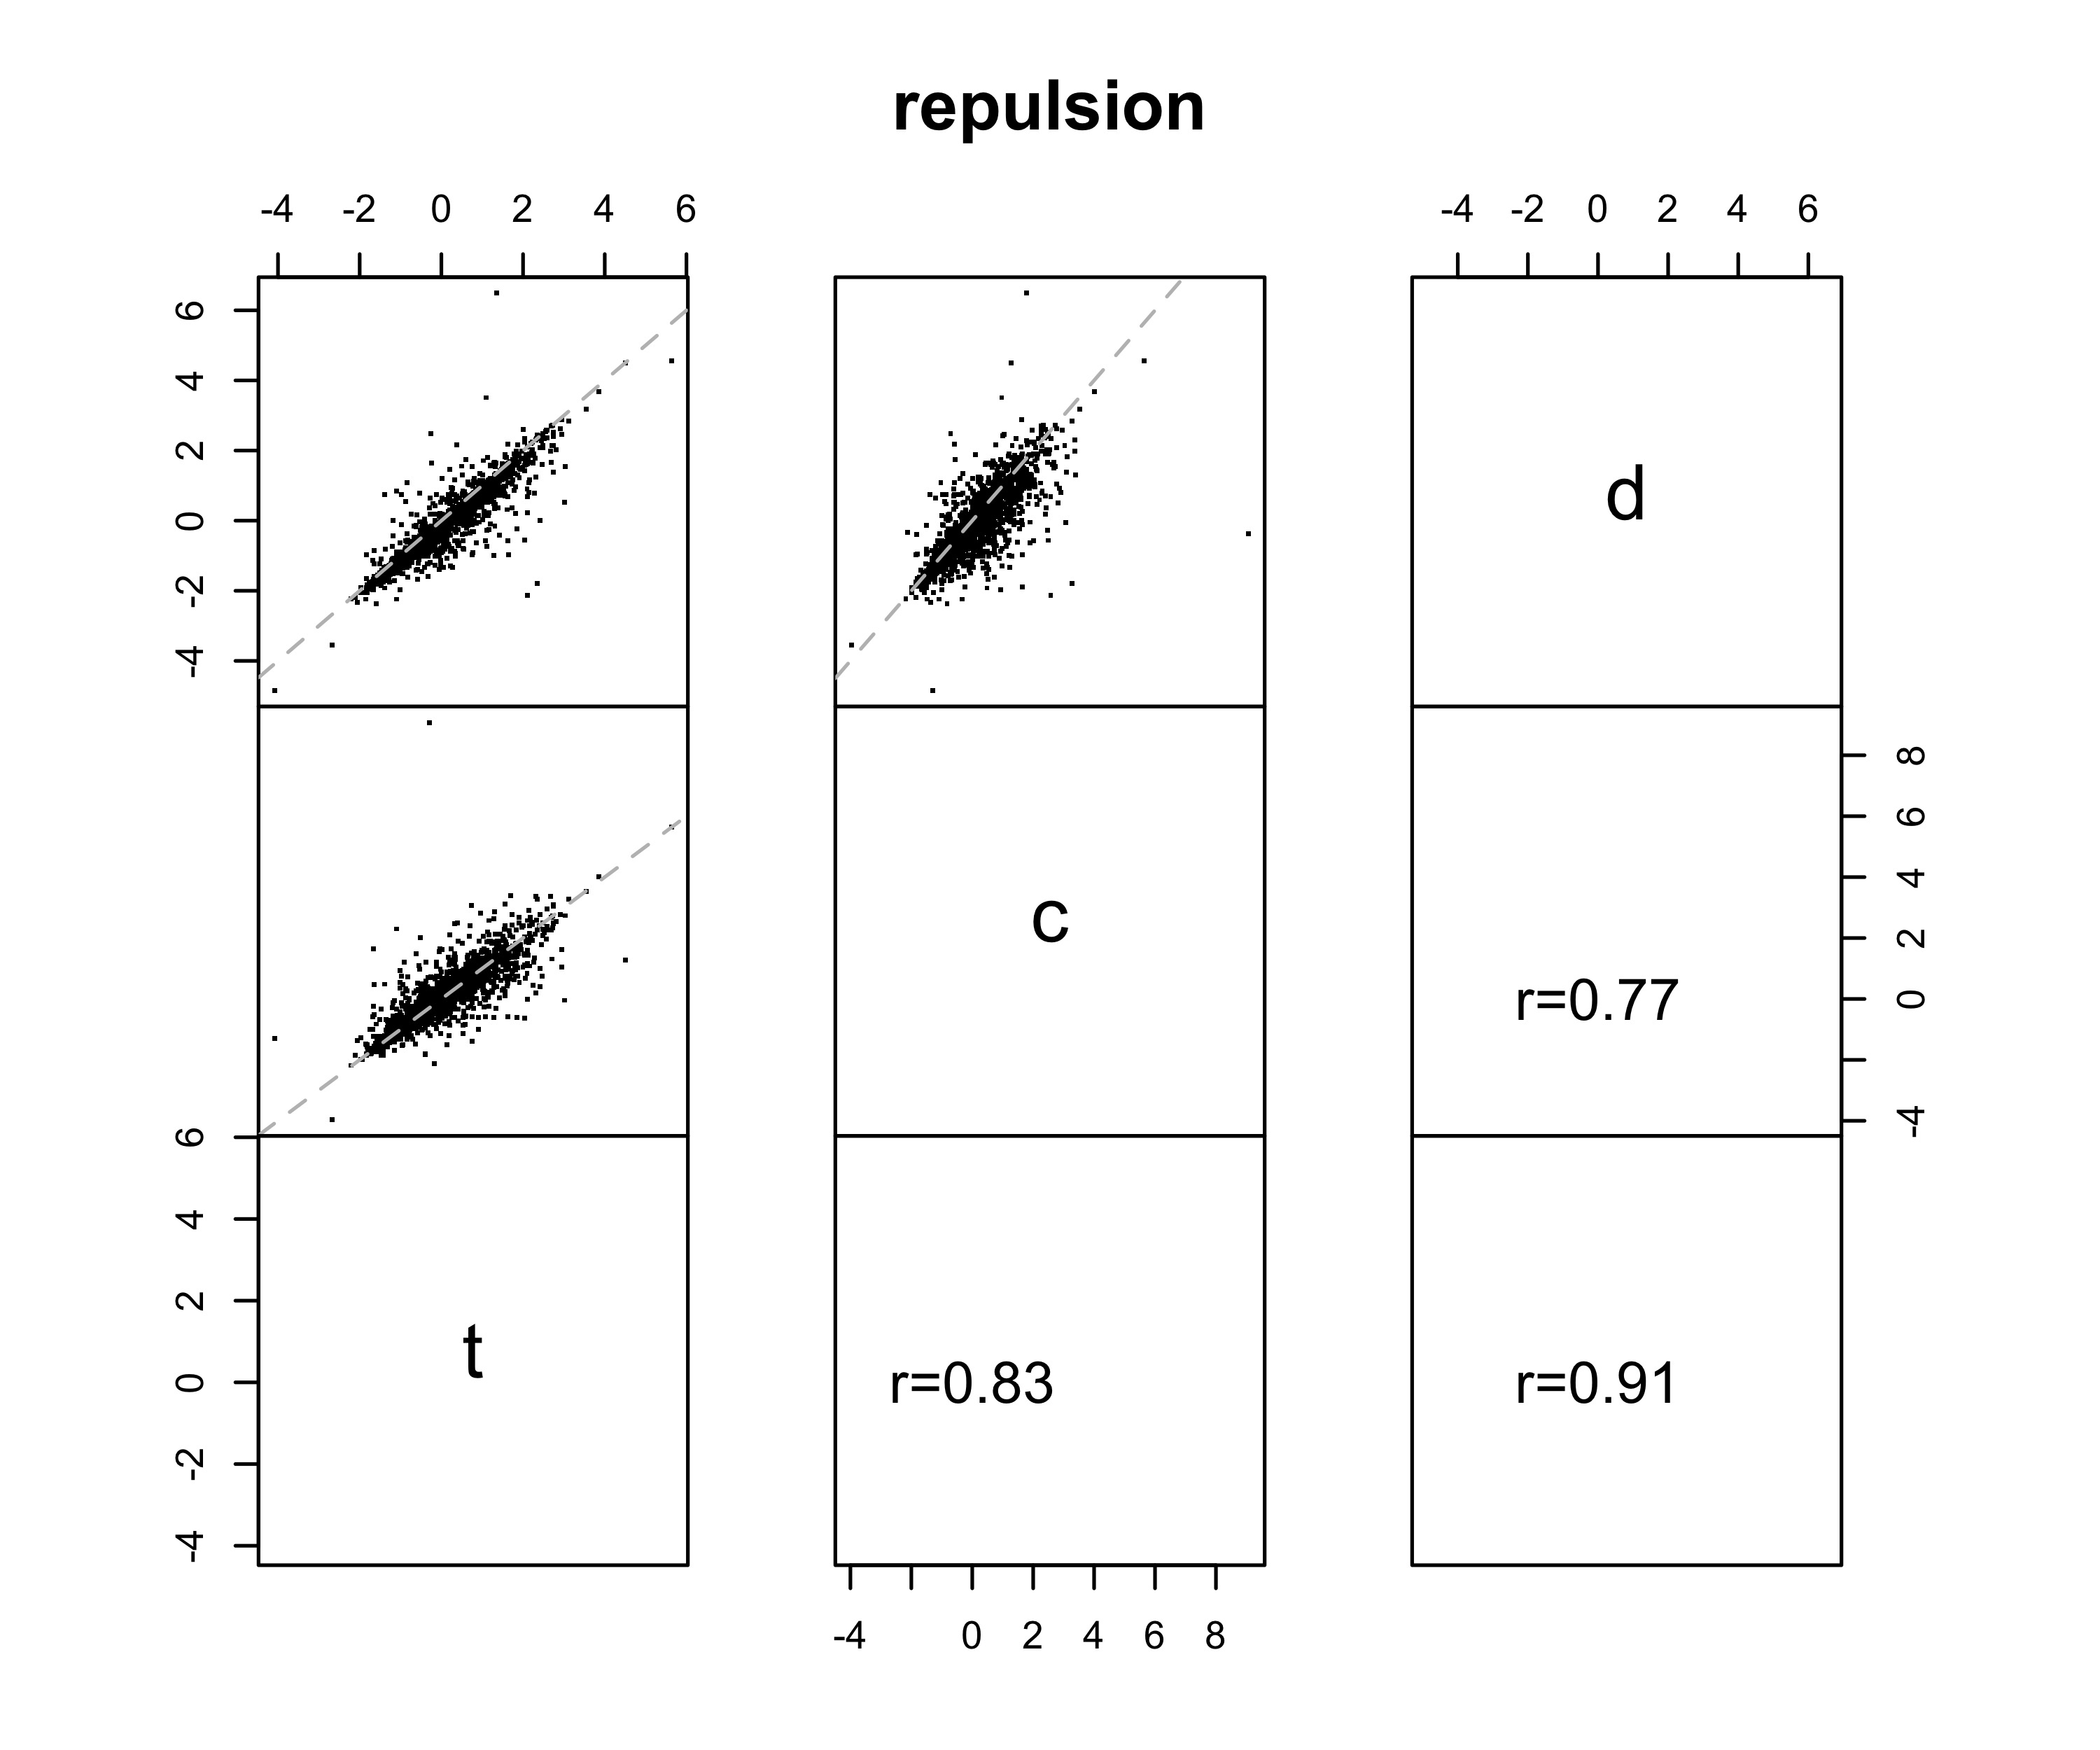
\includegraphics[scale=.5,width=120mm]{figures/price_z_corplot_repulsion.jpeg}
    \caption{Experiment 4 correlation plots for all pairs of stimuli, in trials designed to elicit the repulsion effect. t=target, c=competitor, and d=decoy.}
    \label{fig:price_z_corplot_repulsion}
\end{figure}

\begin{figure}
    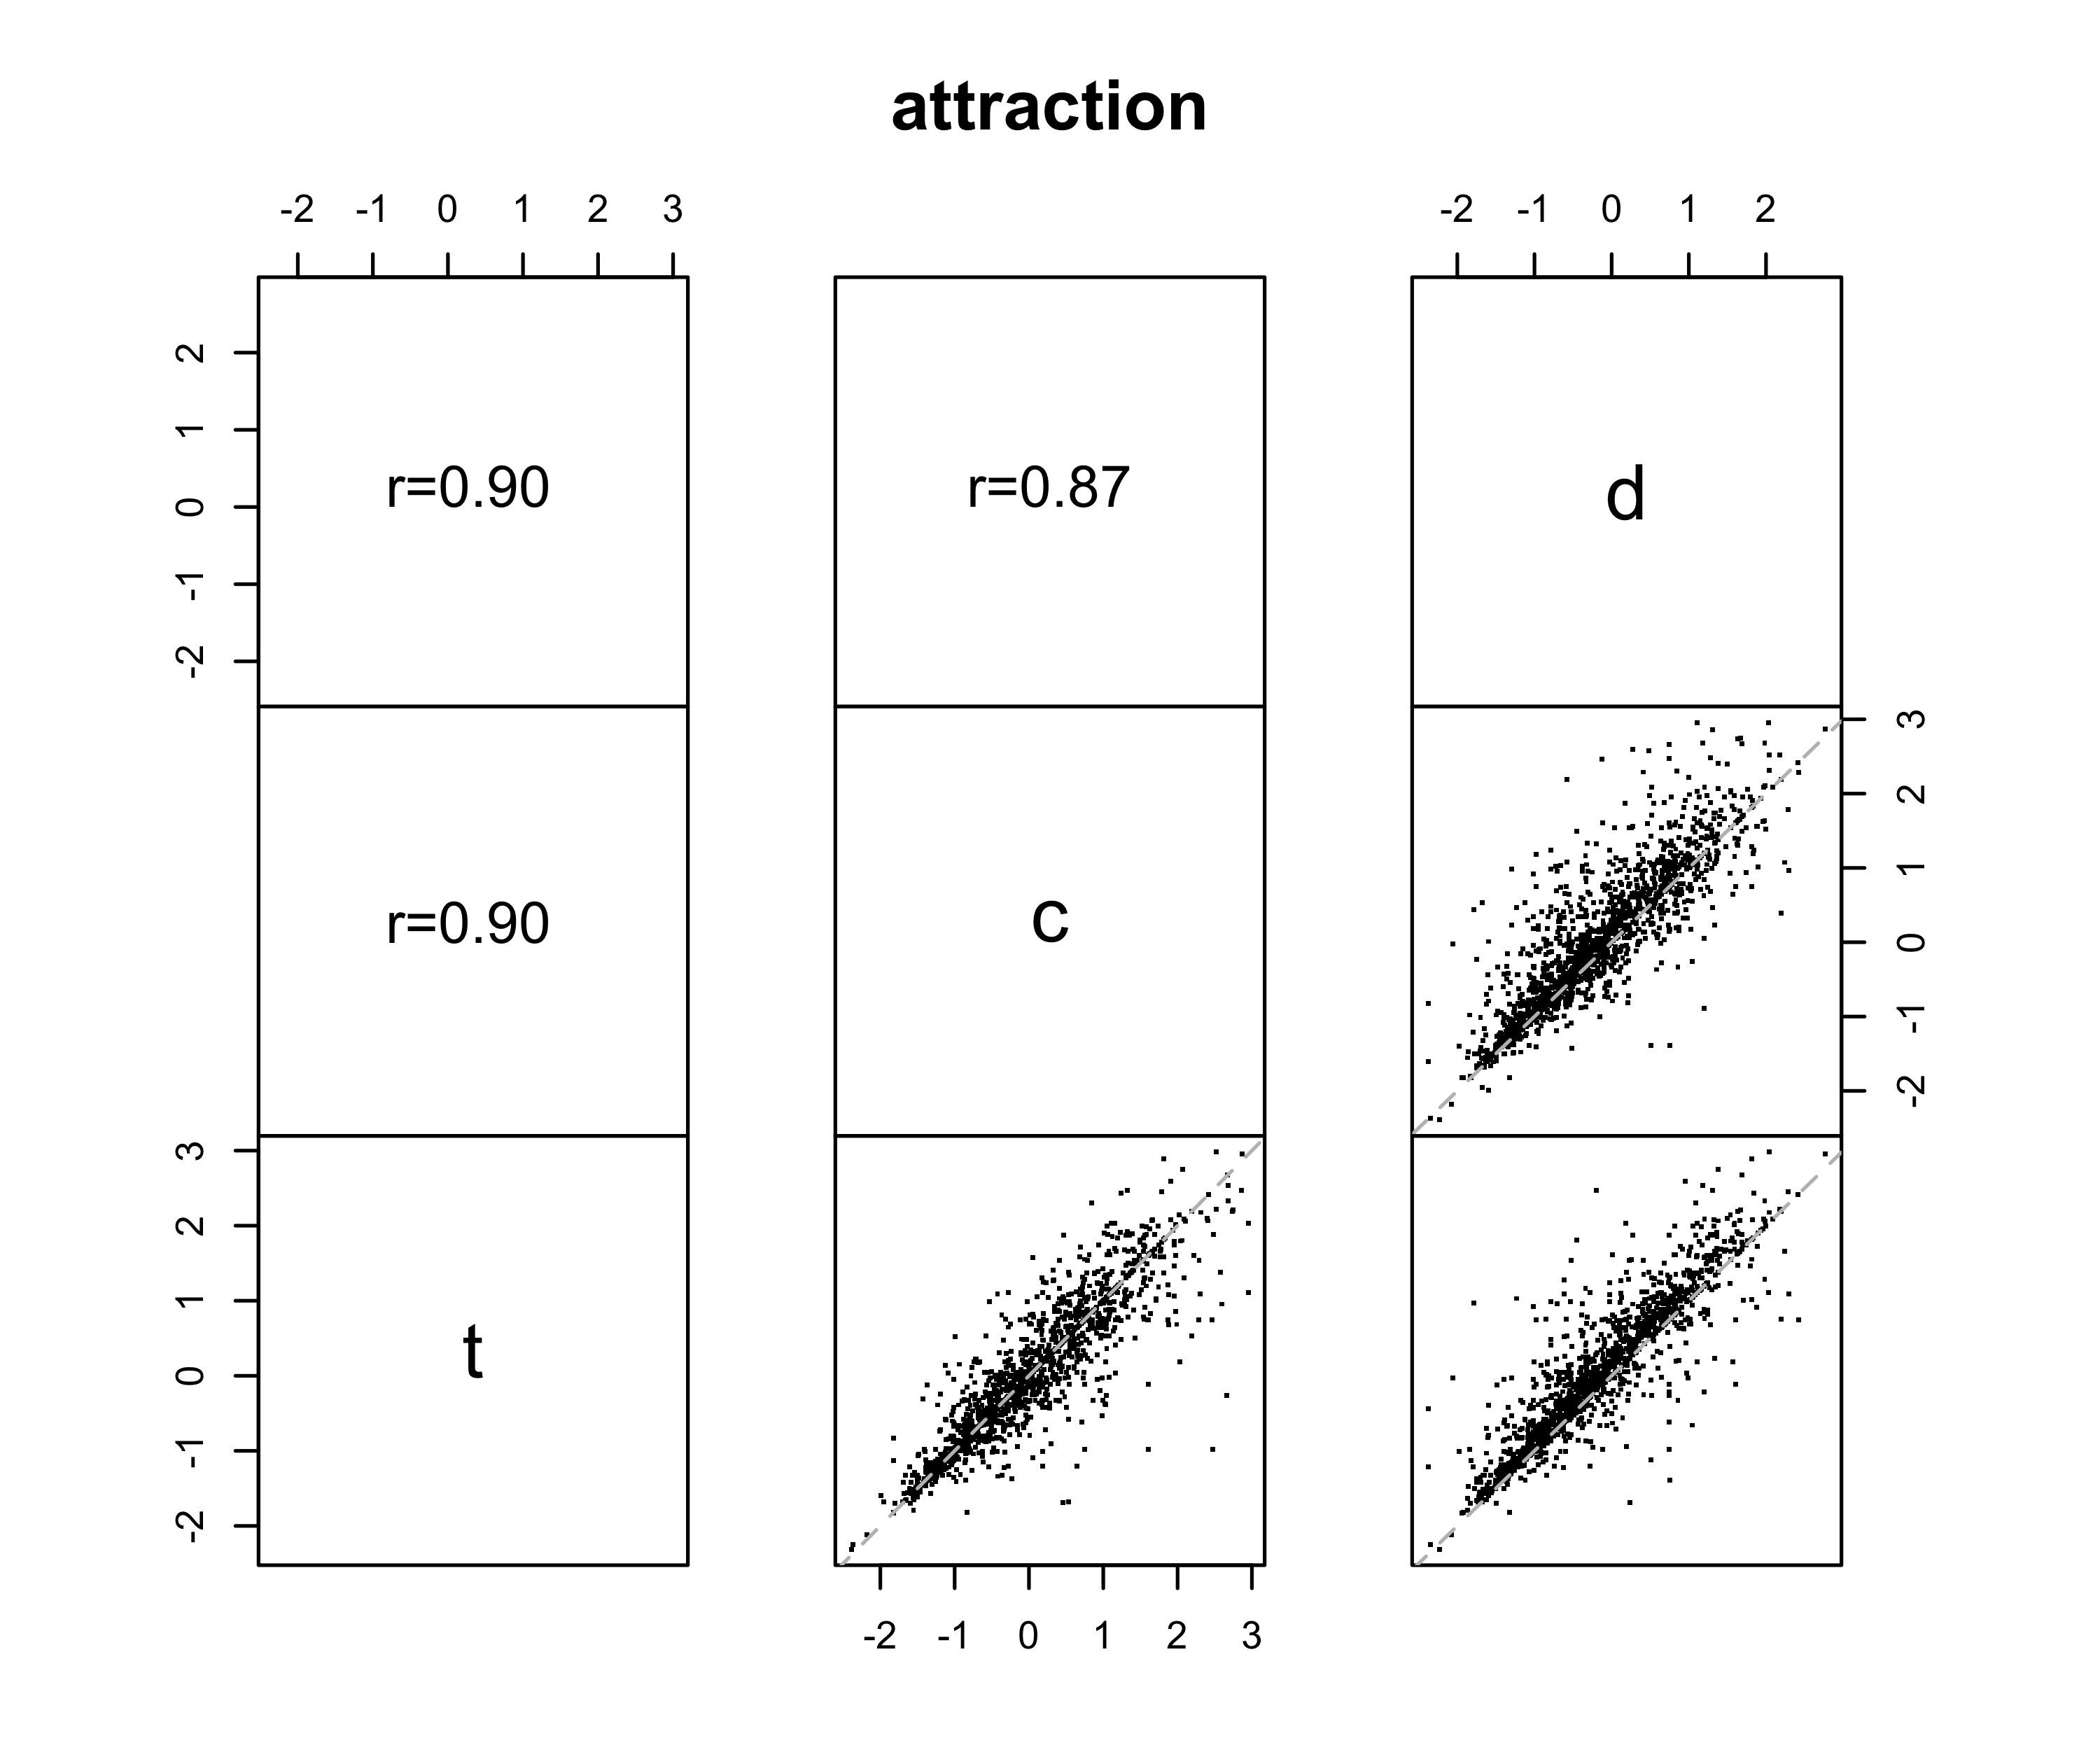
\includegraphics[scale=.5,width=120mm]{figures/price_z_corplot_attraction.jpeg}
    \caption{Experiment 4 correlation plots for all pairs of stimuli, in trials designed to elicit the attraction effect. t=target, c=competitor, and d=decoy.}
    \label{fig:price_z_corplot_attraction}
\end{figure}

\subsubsection{Choice Trials}

I next computed choice proportions for the critical choice trials. I collapsed across participant (due to the small $n$ per subject), as well as product category and the target's superior dimension.

These choice proportions are plotted in Figure~\ref{fig:bayes_choice_model_data_plot}. The results clearly show a null attraction effect, regardless of $TDD$. Participants chose the target and competitor options at equal rates. This is likely due to the strong similarity of target and competitor, atypical of attraction effect studies. 

The results show what appears to be a repulsion effect, where the participants generally prefer the competitor option to the target option. However, because I did not include a ternary-ternary comparison (i.e., varying whether the decoy is located nearer to the extreme option or to the intermediate option), these results may be due to participants simply preferring the less extreme option.

Participants seldom chose the decoy, another indication that they were attentive to the task. This also provides evidence that decoy selection is far more common in perceptual choice than preferential choice.

\begin{figure}
    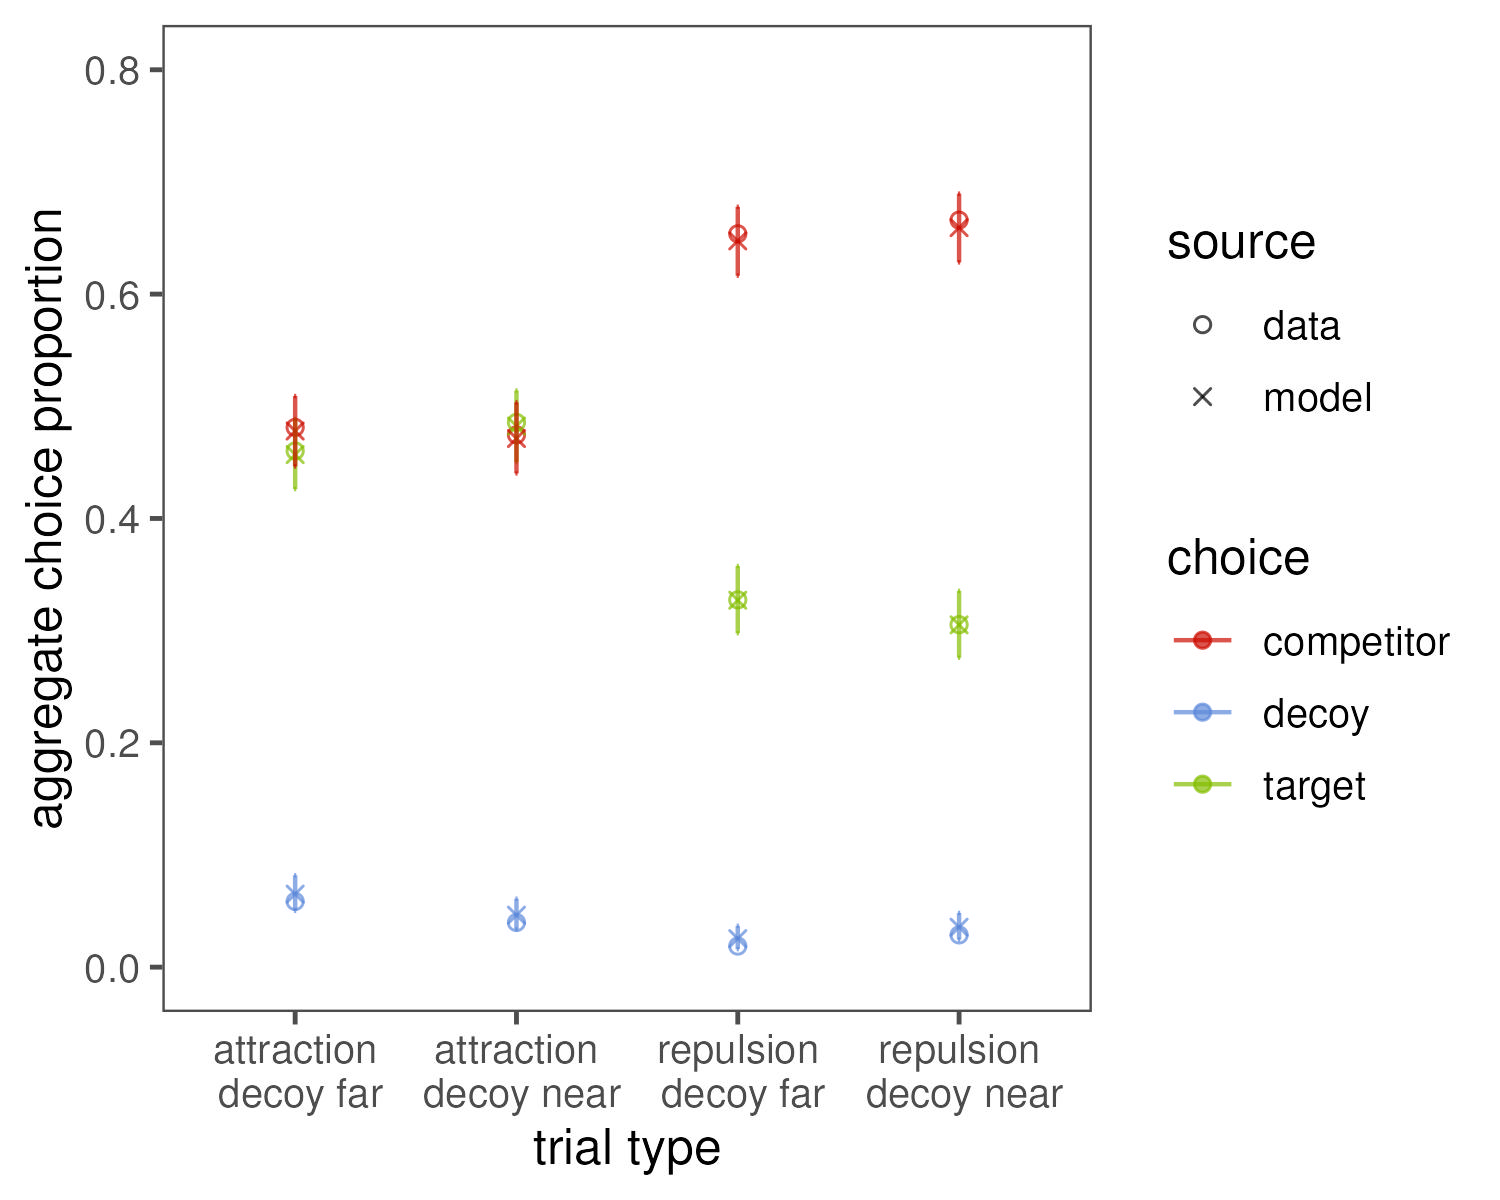
\includegraphics[scale=.5,width=100mm]{figures/bayes_choice_model_data_plot.jpeg}
    \caption{Experiment 4 aggregate choice proportions for each trial type, TDD, and option. Data points are aggregate choice proportions, while model points are posterior means computed from the Bayesian Dirichlet-multinomial model presented in the Appendix. Error bars are $95\%$ HDIs.}
    \label{fig:bayes_choice_model_data_plot}
\end{figure}

\subsubsection{Model Simulations}

As in Chapter 2, I used the parameter estimates for $\boldsymbol{\mu}$ and $\boldsymbol{\Sigma}$ to simulate choice. I use the Thurstonian model from Chapter 2, originally used to simulate perceptual choice. 

To simplify this analysis, I only consider attraction and repulsion trials, collapsing over all other factors. 

As in Chapter 2, the model assumes that value is stochastic while choice is deterministic\footnote{This also assumes ties are not possible, which is true if and only if perceived area is absolutely continuous.}. The model always chooses the option perceived as most valuable, regardless of the magnitude of the difference between the "winner" and "runners-up". That is, given a vector $\mathbf{X}_i$ of perceived values on trial $i$ with set $K$, the probability a participant selects stimulus $j$ is:

\begin{align}
   P(j|i,K)=P(\mathbf{X}_{ij}>\mathbf{X}_{ik}), \forall k \in K, j \neq k
   \label{eqn:pchoice_price}
\end{align}

I ran $1,000,000$ simulations of the model and plotted the results against the data in Figure~\ref{fig:bayes_choice_sim_preds}.

\begin{figure}
    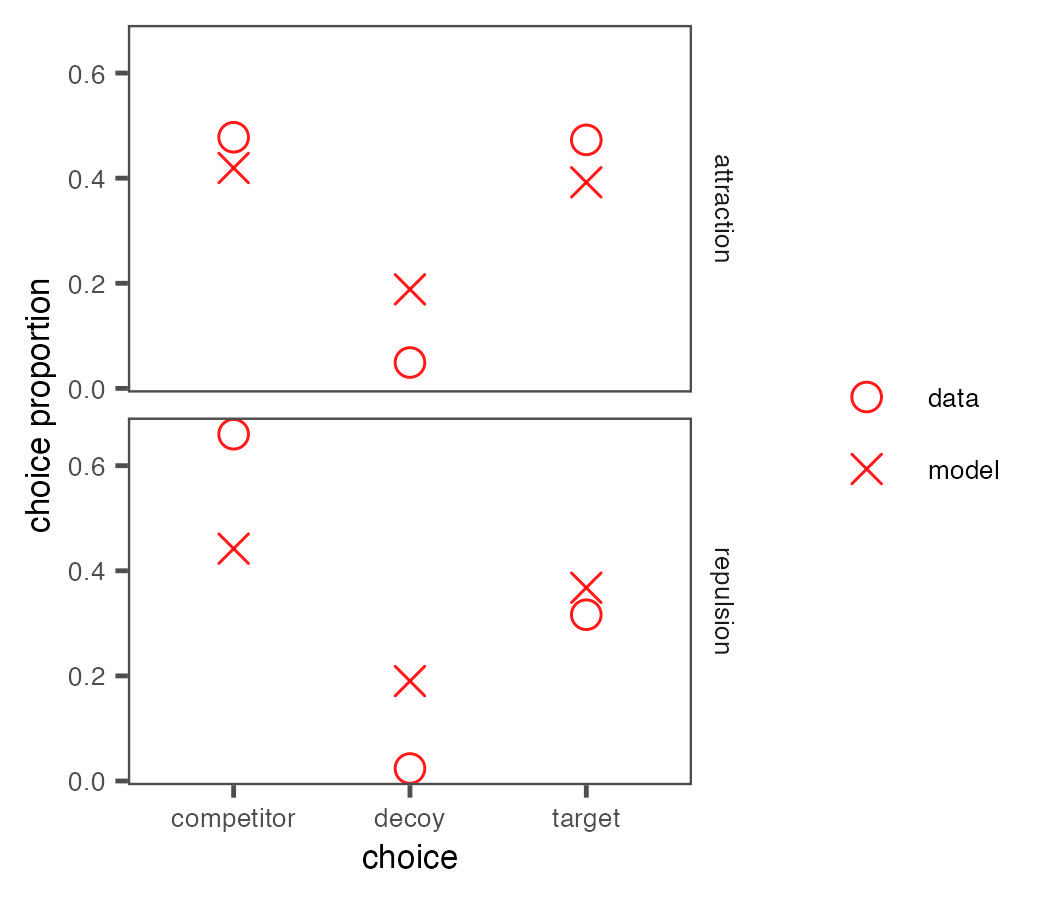
\includegraphics[scale=.5,width=100mm]{figures/bayes_choice_sim_preds.jpeg}
    \caption{Experiment 4 data vs. Thurstonian model predictions.}
    \label{fig:bayes_choice_sim_preds}
\end{figure}

The model mispredicts the attraction trials. It predicts a slight repulsion effect when in fact the data suggest a null effect.

The model successfully predicts a qualitative repulsion effect, i.e., $P(C)>P(T)$. However, it strongly overpredicts decoy choice proportions. The model relies on the correlation between target and decoy choice proportions to predict the repulsion effect. According to the model because the target and decoy are strongly correlated, it is more likely that the utility of the decoy exceeds the target than the competitor. The decoy then "steals" choice shares from the competitor. This prediction makes sense in perceptual choice, where stimulus discriminability is not a given and participants pick the decoy roughly $20$-$30\%$ of all trials (see Experiment 2). In preferential choice, participants almost never pick the decoy, and researchers assume that any participant with sufficient attention can always discriminate the target and competitor from the decoy. Thus, though the model can qualitatively predict a repulsion effect, the mechanism by which it does so is implausible.

\section{Discussion}

This experiment generalizes the paradigm of Chapter 2 to preferential choice. Participants completed two phases; in the first phase, they assigned a selling price to each of three options on each trial. In the second phase, they selected the option they would most prefer. Option sets were designed to either elicit the attraction effect or the repulsion effect. I used the prices to estimate the mean value of each option as well as the correlations between all pairs of options. In doing so, I extended not only the experimental paradigm of Chapter 2, but also the modeling framework, to a preferential choice setting.

Crucially, when estimating the correlations, I replicated the result of Experiment 2, that, in the repulsion effect $\rho_{TD}>\rho_{TC}$ and $\rho_{TD}>\rho_{CD}$. Interestingly, the inferential statistics also show that $\rho_{TC}>\rho_{CD}$. This result was unexpected, but it may be due to the fact that, because both are high on one dimension and low on another, it is easier to compare target and competitor to one another than it is to compare the competitor to the decoy. 

Interestingly, in the trials designed to elicit the attraction effect, I found that $\rho_{TC}\approx\rho_{TD}>\rho_{CD}$. This is likely due to the similarity of target and competitor on both attributes (i.e., one option's dimension values were $[50,60]$ while the other's was $[60,50]$). The target and competitor are easily comparable to one another, and the tradeoff on attributes is negligible.

The choice results replicated those of \textcite{banerjeeFactorsThatPromote2024}, in that participants chose the competitor more than the target in each of the repulsion effect choice sets. However, given that I did not vary the decoy location (i.e., the competitor was always less extreme than the target), nor did I include a binary-ternary choice comparison. These results may be due to a bias for the less extreme option, which happens to be the competitor in this case. Future research should include binary-ternary and ternary-ternary trials to generalize these results.

The strong correlation between target and decoy valuations appears to be a robust finding, holding across perceptual and preferential choice. It is worth exploring, in greater detail, what causes these correlations. 

In the attraction and repulsion effect, the target and decoy are designed such to be more similar to each other than either option is to the competitor. It may be that, by measuring the correlation in valuations, we are actually measuring the \textit{similarity} between options. Indeed, the similarity of target and decoy was a primary motivation for the original demonstration of the attraction effect \parencite{huberAddingAsymmetricallyDominated1982d}. 

These correlations may also be measuring the ease of comparability between pairs of options. Comparability has previously been shown to drive the attraction effect \parencite{noguchi2014attraction,cataldoComparisonProcessAccount2019b}, and several models of context effects rely on comparisons of options on single attributes to generate context effects \parencite{trueblood2014multiattribute,roeMultialternativeDecisionField2001a}. Supporting this hypothesis is the finding that $\rho_{TC}>\rho_{TD}$ in the trials designed to elicit the attraction effect, when the target and competitor were quite similar on each attribute and thus easier to compare.

Future work could test these hypotheses by systematically manipulating option comparability and assessing whether the correlations vary with comparability. I work towards this in Chapter 5 through testing the effect of comparability on choice, but it would be interesting to directly measure correlations in choice environments of varying comparability. 


\chapter{Comparability in Perceptual Choice}
\label{chapter_5}
\section{Introduction}
Thus far, the dissertation has explored perceptual and decisional processes in both perceptual and preferential choice. Experiment 2 showed that stimuli which are more similar to one another, and are thus more easily comparable, generate valuations with stronger correlations. This result holds across both perceptual choice (Chapter 2) and preferential choice (Chapter 4). The comparison process is defined as a cognitive operation where a participant attends to the relative difference between two options on a choice set, typically (though not necessarily) on a single dimension. 

Embedded in a Thurstonian choice model \parencite{thurstone1927law}, and conditional on parameters estimated from Experiment 2 data, these correlations can produce the repulsion effect \parencite{spektorWhenGoodLooks2018b,simonson2014vices} because the decoy option, whose value is tightly correlated with the target, occasionally exceeds the target in perceived value and thus takes choice shares away from the target. The model can also predict the attraction effect, but parameters estimated from actual empirical data do not predict the attraction effect.

In this chapter, stimulus comparability is manipulated directly in a perceptual choice task. The goal of this manipulation was to empirically test the relationship between comparability and choice. First, the previous literature on comparability is reviewed, and then the results of a perceptual choice experiment are presented.

\subsection{Previous Literature on Comparability}

Other researchers have studied the comparison process in decision-making, particularly in high-level choice (e.g., preferential). Below, relevant preferential choice research is introduced before transitioning to relevant research on perceptual choice. 

\textcite{changWhichCompromiseOption2008} tested the compromise effect by varying the presentation of options. In the compromise effect, a middle-ground option decreases the choice share of two dissimilar, extreme options. \textcite{changWhichCompromiseOption2008} displayed the options either by-alternative format, where option names are listed as columns while attribute values are listed as rows, or by-attribute, where option attributes are columns while option names are rows. The former display makes it more difficult to compare options on a single attribute, while the latter makes it easier. \textcite{changWhichCompromiseOption2008} found that listing options by-attribute increased the choice share of the compromise option, relative to a by-alternative display. 

\textcite{cataldoComparisonProcessAccount2019b} replicated this result, also finding that a by-alternative format nullified the attraction effect. The authors attributed this result to a flexible comparison process, where the comparison strategy is influenced by display format. According to this account, the by-attribute format increases the ease of target-decoy comparisons relative to the by-alternative format. 

\textcite{noguchi2014attraction} studied context effects using eye-tracking, showing that people tend to compare pairs of options on a single attribute, and that this appears to drive the attraction, similarity, and compromise effect. In their study, participants' eye movements showed that they were more likely to transition between options on a single dimension than they were to transition between dimensions within a single option. They also found that transitions between two options are negatively related to the choice share of a third option.

\textcite{hayes2024attribute} manipulated attribute comparability, such that the dimensions of each option were either measured in the same unit (high comparability, e.g., 0-10 ratings on all attributes) or in different units (low comparability, e.g., CPU speed vs. RAM for laptops). They found that the attraction effect only occurred in the low comparability condition. 

\textcite{hasan2025registered} conducted a large scale replication factors that impact the attraction effect, systematically varying option order, presentation mode (numerical or graphical), and presentation format (by-attribute or by-alternative). They found that the attraction effect was stronger when the target and decoy options were adjacent to one another, presumably because this allows for easier target-decoy comparison. The attraction effect was stronger when attributes were presented numerically compared to graphically, a result found by other researchers \parencite{frederickLimitsAttraction2014b,yangMoreEvidenceChallenging2014}. They did, however, fail to replicate \textcite{cataldoComparisonProcessAccount2019b}'s finding that the attraction effect varies with by-alternative vs. by-attribute format.
% , albeit with different decoy types. In \textcite{cataldoComparisonProcessAccount2019b}'s original study, the decoy was wors

Hsee and colleagues \parencite{hseeEvaluabilityHypothesisExplanation1996,hseeLessBetterWhen1998,hseeWillProductsLook1998,hsee1999preference} have also shown that the comparison of options affects consumer behavior. For example, they repeatedly showed that participants’ evaluation of a given option can change with the addition of a reference point. For example, lower valued options improve with a high reference point and vice versa. Participants’ judgments can reverse when options are evaluated jointly, compared to separately \parencite{hsee1999preference}. 

Several computational models of decision-making also rely on the comparison process.  \textcite{roeMultialternativeDecisionField2001a}'s Multialternative Decision Field Theory (MDFT) model also assumes that options accumulate evidence through comparison, and that comparisons between nearby options exhibit greater influence on preference. According to \textcite{trueblood2014multiattribute}'s Multiattribute Linear Ballistic Accumulator Model (MLBA), each option accumulates evidence through pairwise comparisons to all other available options. These comparisons are modulated by several processes, such as distance in attribute space and extremeness aversion. Other decision models incorporate similar mechanisms \parencite{usherLossAversionInhibition2004a,noguchiMultialternativeDecisionSampling2018a,spektor2019similarity,wollschlager2NaryChoiceTree2012a,landry2021pairwise} (c.f. \textcite{bhatiaAssociationsAccumulationPreference2013b,bergnerVAMPVotingAgent2019b}). 

\textcite{trueblood2022attentional} argued that pairs of similar options garner more attention in the comparison process. They presented a simple Markov model where pairwise comparisons on a single attribute determine the accumulation of preference, and the time spent on a comparison is an increasing function of the similarity of options on the attribute. Their model can successfully, and simply, account for the "big three" context effects (attraction, compromise, and similarity).

\subsection{Comparability Effects in Perceptual Choice}
There has been other research, albeit relatively limited, studying the comparison process in perceptual decision-making. Much of this work has focused on the spatial layout of the options and its effect on perceptual context effects.

\textcite{trueblood2022attentional} re-analyzed previous perceptual choice context effect data \parencite{trueblood2015fragile} by examining the order of the options presented to participants. They found that the attraction effect was strongest when the target and decoy were next to each other, while the effect was weak (or even absent) when the options were separated spatially. Their conclusion, supported by a modeling analysis, was that people tend to compare pairs of options which are spatially closer to one another more often than pairs further away from one another. 

\textcite{evansImpactPresentationOrder2021} found a similar result in perceptual choice, though in their experiment the options were separated both spatially and temporally. In their experiment, participants saw three rectangles, presented sequentially, and selected the largest rectangle after all stimuli were presented. They found that orders in which the target and decoy were presented in the latter two positions elicited an attraction effect, whereas orders in which the competitor and decoy were presented in the latter two positions tended to elicit a repulsion effect. They interpreted their results as evidence that the comparison process can be altered through spatial and temporal properties of the stimuli.

Another interpretation of their results, and those of \textcite{trueblood2022attentional}, is that by altering the location and timing of the stimuli, the researchers are also altering the comparability. In the Thurstonian model of Chapter 2, increased comparability is represented by an increase in perceptual correlation. As shown previously, this perceptual correlation can create a repulsion effect by allowing the decoy to more easily take choice shares from the target.

This chapter extends the work of Chapter 2. The Thurstonian model from Chapter 2 predicts that when two options (target and competitor) are on average equally viable, but if the target and decoy perceptions are more strongly correlated than competitor and decoy perceptions, participants will choose the target less than the competitor. In Experiment 2, this correlations occur because the target and decoy are perceptually similar (i.e., oriented identically). In this Chapter, however, the decoy is equally similar to both focal options, but the correlation between decoy and target is now created through comparability.

The goal of this experiment was to isolate the effect of comparability from standard context effects. A simple perceptual choice experiment is presented, where participants saw three rectangles at a time and were told to select the largect rectangle. On critical trials, two of these rectangles were equally large but oriented differently (i.e., \textit{focal} rectangles, as in Experiments 1, 2, and 3). A third \textit{decoy} option was a symmetrically dominated decoy - equally similar to either option. One of the two focal options as the \textit{target} based on its proximity and comparability to the decoy. 

To manipulate comparability, the positioning of the options on screen was systematically manipulated. Options were displayed in one of four ways: all aligned in a horizontal line, as in \textcite{trueblood2013not}; two adjacent options aligned vertically, with a third option positioned in a different vertical location; and the triangle alignment from \textcite{spektorWhenGoodLooks2018b}. See Figure~\ref{fig:comparability_trials} for example stimuli.

Proximity is defined as closeness in space, and comparability is defined as the ease of comparison between two stimuli. The critical display is the two-aligned condition, where the target and decoy are positioned such that they are easily compared, while the competitor is located where comparisons are more difficult. Based on the results of Chapter 2, ease of comparability should increase the correlation between the target and decoy and result in a \textit{decrease} in the target's choice share in the two-aligned condition, relative to the none aligned and all aligned conditions. In the model and experiment presented in Chapter 2, the similarity of the target and decoy caused the decoy to take choice shares away from the target. Here, both focal options are equally similar to the target, but the target is located closer to the decoy and is more comparable. These predictions are generally borne out in the data, albeit with limitations which will be discussed below.

\section{Experiment 5}
Experiment 5 adresses the effect of comparability in perceptual choiceusing \textit{symmetrically dominated} decoys. A symmetrically dominated decoy is dominated by both focal options but is also equally similar to both options. Thus, the terms target and competitor, which have been used throughout this dissertation, take on a different meaning here. Here the target is defined as the option that is both adjacent to and easily comparable to the decoy. Based on the experimental and modeling results of Chapter 2, it was predicted that the choice share of the target will be reduced when it is particularly comparable to the decoy.

\subsection{Methods}

\subsubsection{Participants}
$231$ undergraduate students at the University of Massachusetts Amherst participated in the lab, in exchange for course credit. $17$ participants' data were removed from all analyses because they failed to achieve at least $80\%$ correct on catch trials (see below), leaving a final sample size of $N=214$. 

\subsubsection{Stimuli}
The stimuli were gray-scale rectangles and squares, varying systematically on height and width. 

The critical stimuli are depicted in Figure~\ref{fig:comparability_stim_plot}. The focal stimuli ($H$ and $W$) are equal in area and fell on two diagonals, the upper diagonal area being $25000$ square pixels and the lower diagonal being $7581\text{px}^2$. On the lower diagonal, the focal stimuli had dimension values of $57$ and $133$ pixels, while on the upper diagonal, the the focal stimuli had dimension values of $127$ and $141$ pixels. 
The decoy options were either $20\%$ or $35\%$ smaller than the focal options. This was determined based on the results of pilot data and with the goal of making the decoy somewhat difficult to discriminate from the focal options. For the manipulation to work, participants needed incentive to consider the decoy and thus to compare it to the two focal options. 

\begin{figure}
   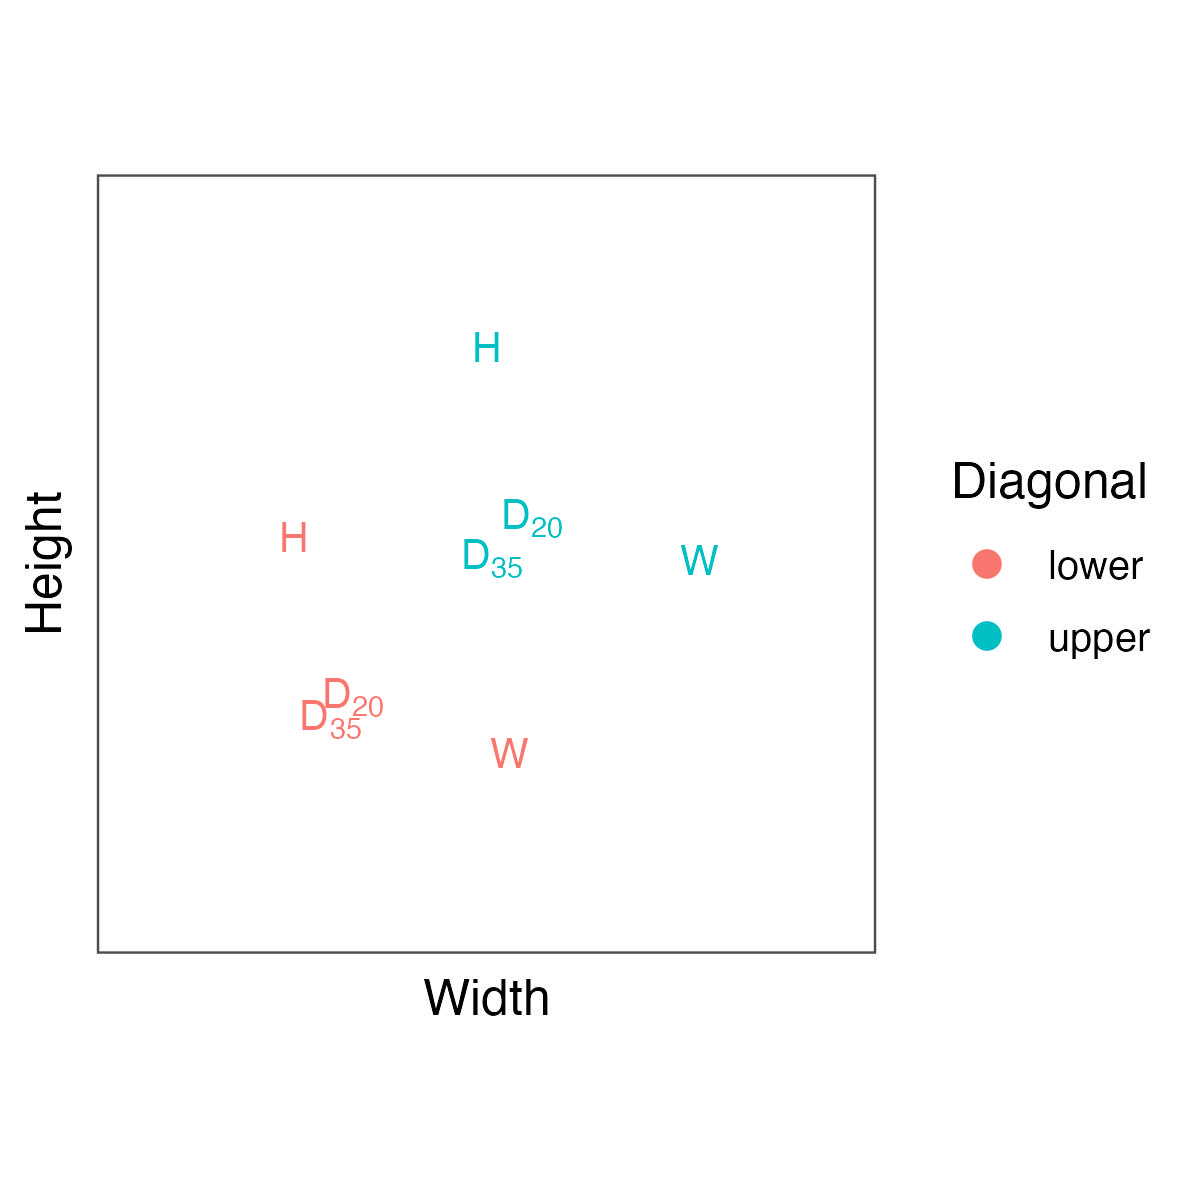
\includegraphics[width=100mm]{figures/comparability_stim.jpg}
   \caption{Graphical depiction of critical stimuli from Experiment 5. The stimuli fall on two diagonals, referred to as upper and lower. The H rectangles are taller than wide, while the W rectangles are wider than tall. The decoy (D) rectangles are equally wide and tall (i.e., squares). The decoy subscripts indicate the $TDD$ $\%$.}
   \label{fig:comparability_stim_plot}
\end{figure}

% On each critical trial, there were three options: an $H$ rectangle, a $W$ rectangle, and a $D$ rectangle. The focal rectangles fell on two diagonals (upper and lower, see above), while the decoy rectangle varied in $TDD$ at $20\%$ and $35\%$. 

The stimuli were arranged in one of four displays: all-aligned, two-aligned, none-aligned, or triangle. See Figure~\ref{fig:comparability_trials} for sample trials. 

In the all-aligned display, all stimuli were arranged in a horizontal array, as in the experiments of \textcite{trueblood2013not} and \textcite{spektorWhenGoodLooks2018b}, Experiment 4.

In the two-aligned display, two options were aligned horizontally in the top-left and top-middle positions, while the third option was placed in the bottom-right position of the screen. This is a crucial condition and an instantiation of the comparability hypothesis, in which the comparison of the two aligned options is far easier than all other pairwise comparisons.

In the none-aligned display, all options are located in different vertical and horizontal positions, such that all comparisons should be more difficult, as determining the relative areas between rectangles is no longer straightforward.

The triangle display is identical to the triangle display of Experiments 1 and 2, with the exception that on half of all triangle display trials, the triangle was inverted. Note that this is distinct from the two aligned condition, as the options are located in distinct vertical and horizontal positions and it is difficult to determine the relative sizes between rectangles. 
% The triangle display condition was collected for future analyses but is not germane to the current research question, and it will be excluded from critical analyses.

In all displays, the horizontal distances between all options was constant.

In addition to varying diagonal, $TDD$, and display, option order also varied, such that all six orders ($DHW$, $DWH$, $HDW$, $HWD$, $WDH$, and $WHD$) were equally common.

\begin{figure}
   \begin{center}
      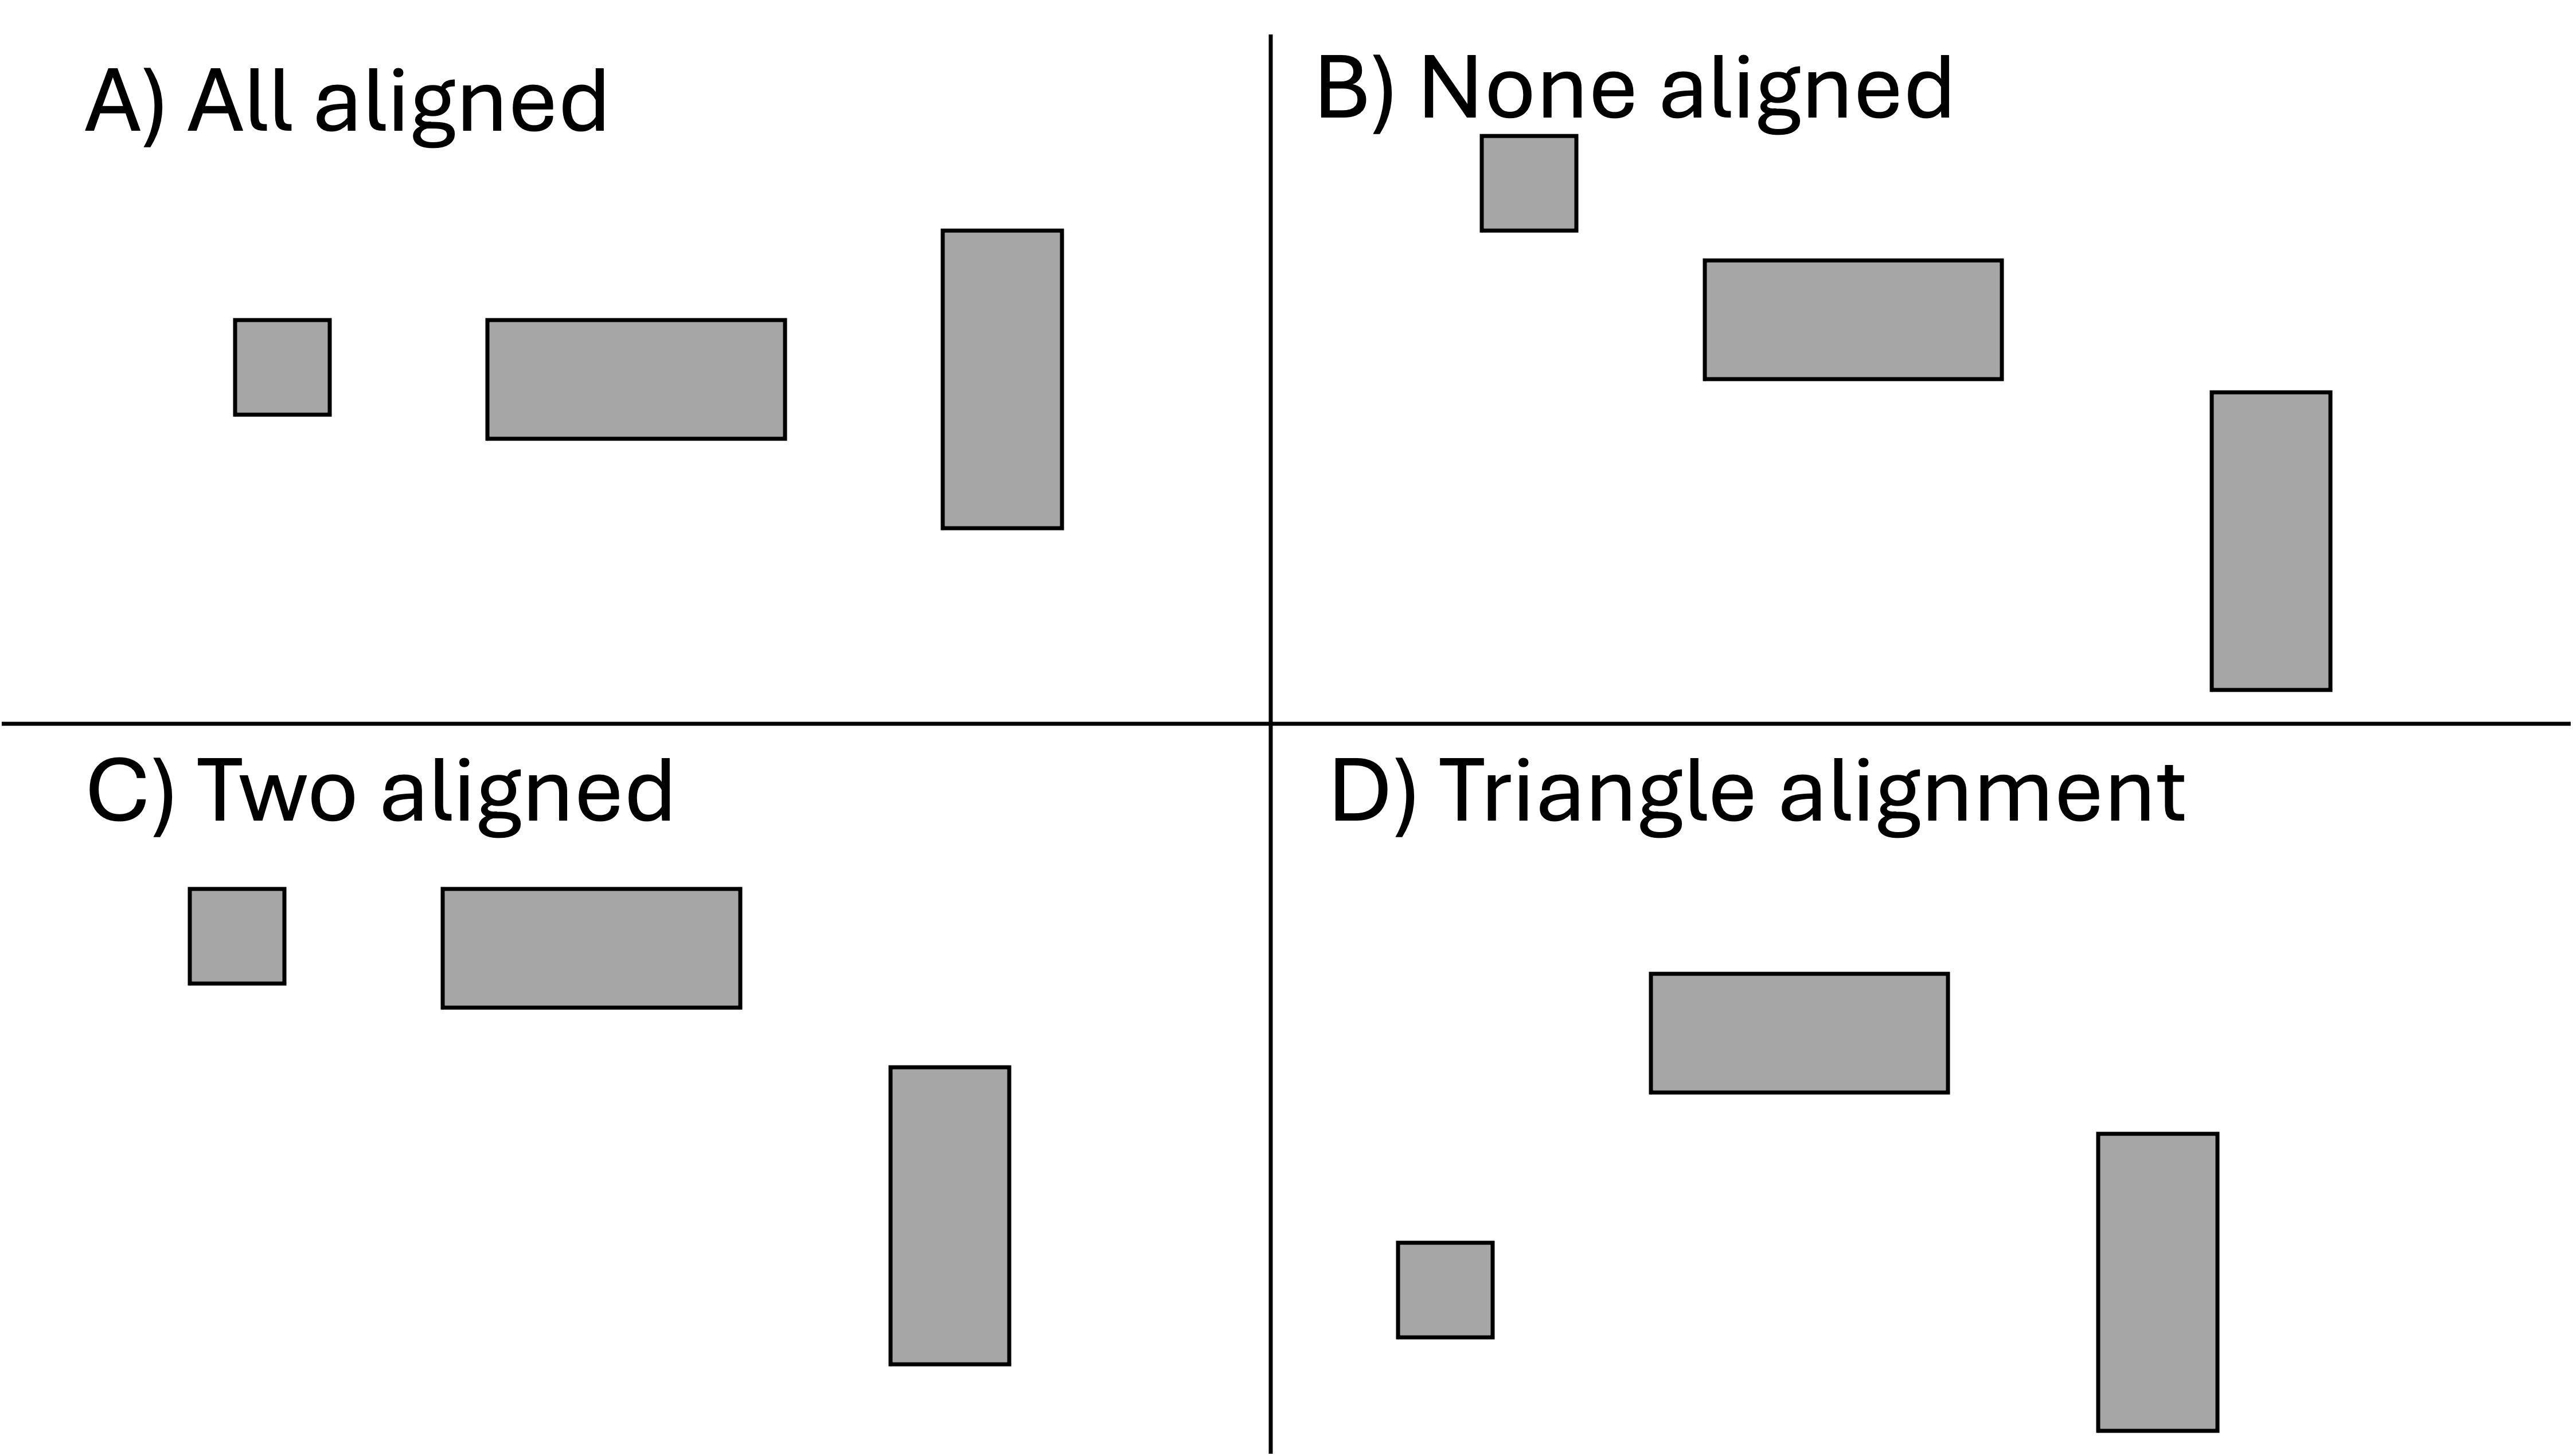
\includegraphics[width=100mm]{figures/comparability_design.jpg}
      \caption{Sample critical trials from Experiment 5. A) all aligned. B) Two aligned. C) None aligned. D) Triangle alignment.}
      \label{fig:comparability_trials}
   \end{center}
\end{figure}

There were other types of stimuli on non-critical trials: filler-random, filler-square, and catch.

On filler-random trials, three options were randomly generated by sampling a height and width from the $U(57,200)px$ distribution. Filler-random trials were included to avoid participants noticing the manipulation on the critical trials and to include enough challenging trials to keep participants engaged in the task.

On filler-square trials, a square was randomly generated by sampling a side length from the $U(57,200)px$ distribution. Then, two non-square rectangles were generated by sampling a height and width from a the $U(57,S)px$ distribution, where $S$ is the side length for the square. This manipulation ensured that the square was always the largest option on these trials. These trials were included to ensure that participants did not learn to ignore the squares, as the critical trials rely on participants comparing the squares to the focal options. 

On catch trials, one large option was randomly generated by randomly sampling a stimulus from the upper diagonal (see Figure~\ref{fig:comparability_stim_plot}). Two smaller options were randomly sampled from the lower diagonal. 

\subsubsection{Design}
As discussed above, there were four types of trials: critical trials, filler-square trials, filler-random trials, and catch trials. The study took place in four blocks.

This was a $2$ (diagonal: lower, upper) x $2$ ($TDD$: $20\%$, $35\%$) x $4$ display: (all-aligned, two-aligned, none-aligned, triangle) x $6$ (order: $DHW$, $DWH$, $HDW$, $HWD$, $WDH$, and $WHD$) within-participants study. Each participant completed $4$ trials for all combinations of these factors ($1$ per each of the four blocks), except for the two-aligned trials, for which they completed $8$ trials ($2$ per each of the four blocks). Thus, there were a total of $480$ critical trials ($(2*2*3*6*4)+ (2*2*1*6*8)=480$).

On each of the non-critical trials, stimulus order was randomized. Additionally, one of the four displays (all-aligned, two-aligned, none-aligned, triangle) was selected at random.

There were $40$ filler-random trials per block for each of four blocks, leading to a total of $160$ filler-random trials. There were $40$ filler-square trials per block for each of four blocks, leading to a total of $160$ filler-square trials. There were $10$ catch trials per block for each of four blocks, leading to a total of $40$ catch trials.

There were a total of $840$ trials in the experiment ($480$ critical + $160$ filler-random + $160$ filler-square + $40$ catch=$840$).

\subsubsection{Procedure}
On each trial, participants saw three rectangles, labeled `1', `2', and `3'. Participants were told to select the largest rectangle. They made their choice by pressing the corresponding key on the keyboard. 

As mentioned above, the experiment was split into four blocks. There was a 15-second break between blocks.

\subsection{Results}

\subsubsection{Data Processing}
In addition to removing participants who failed to meet the $80\%$ correct criterion for catch trials, $2,319$ trials with RTs $<100ms$ or $>10,000ms$ were removed from all analyses. 

\subsubsection{Catch and Filler Trials}
On average, participants performed well above chance on the catch, filler-random, and filler-square trials, including on all display types. See Figure~\ref{fig:comparability_non_crit_mean_prop_correct} for data.

\begin{figure}
   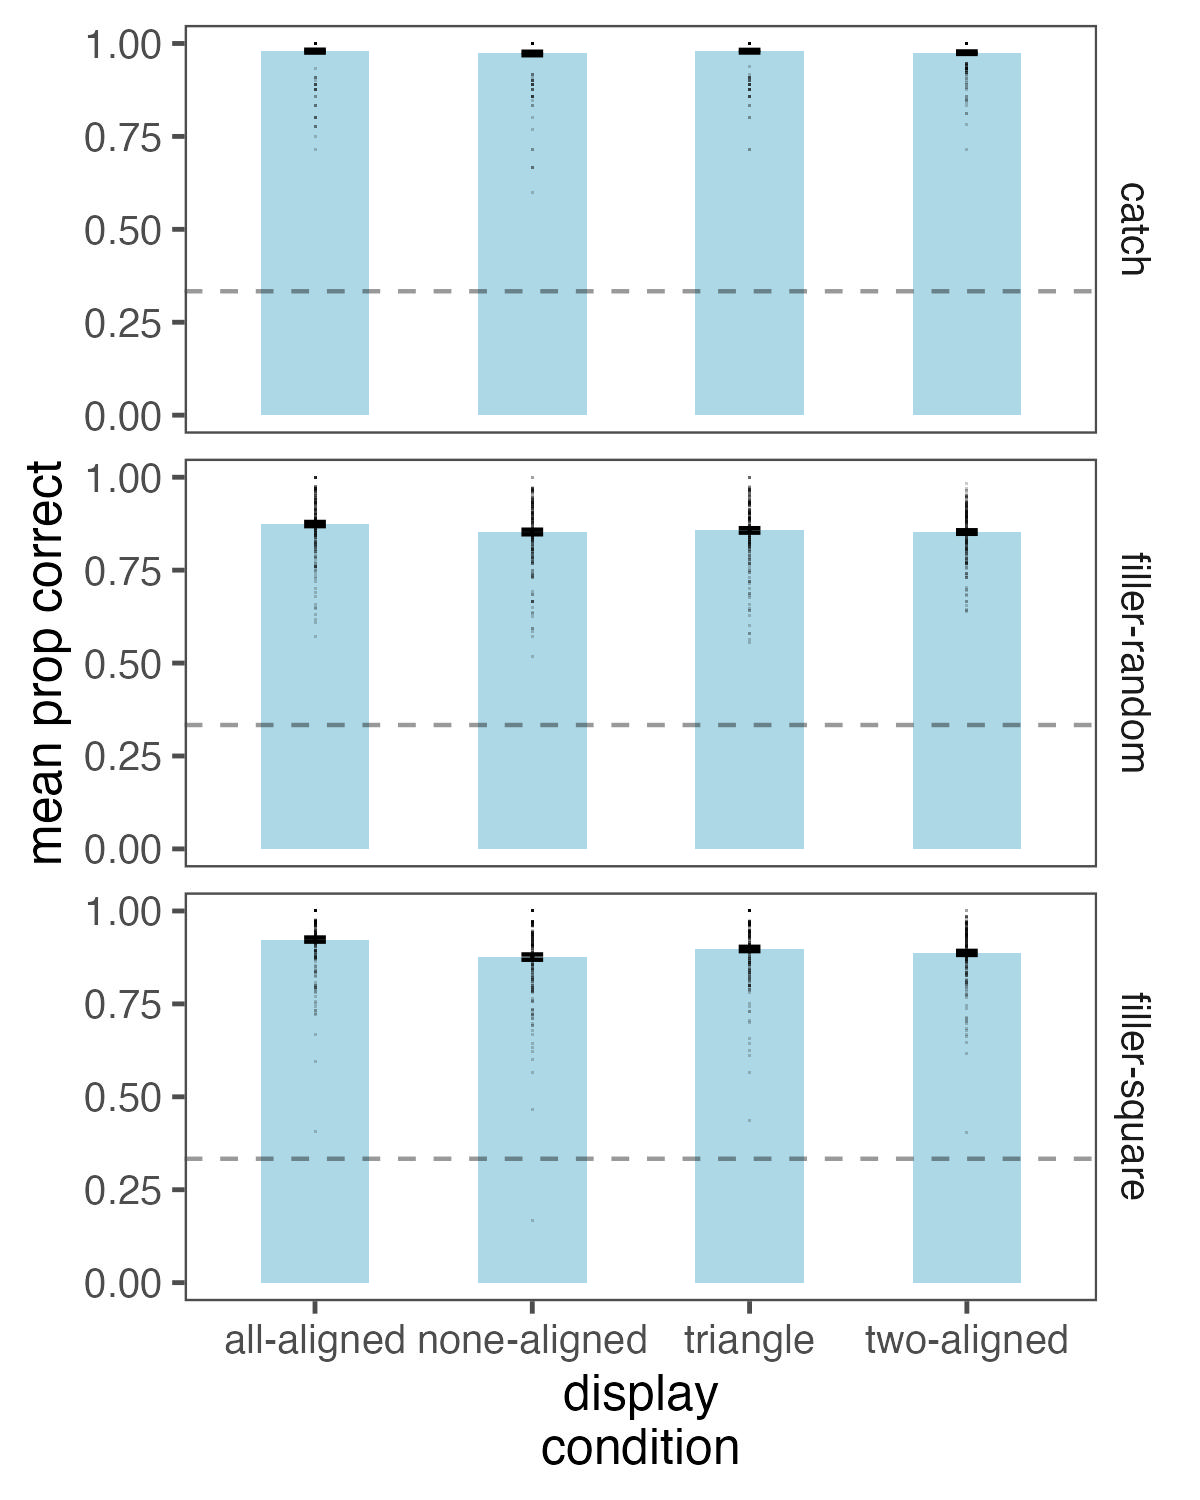
\includegraphics[width=100mm]{figures/non_crit_mean_prop_correct.jpeg}
   \caption{Results from non-critical trials in Experiment 5. Rows show trial types. Bars show mean proportion correct in a given condition, with the error bars showing $\pm1\;\text{SEM}$. Dots show individual participant data. Dashed line is at $1/3$ (chance performance).}
   \label{fig:comparability_non_crit_mean_prop_correct}
\end{figure}

As will be relevant below, participants showed position biases. The order of stimuli on each trial was random, so on average, participants should be equally likely to select the left, middle, rightmost rectangle. However, participants tended to select the middle rectangle the most, followed by the rightmost rectangle, followed by the leftmost rectangle. This bias occured in each configuration. Mean choice proportions for each position for all non-critical trials are plotted in Figure~\ref{fig:comparability_pos_bias}

\begin{figure}
   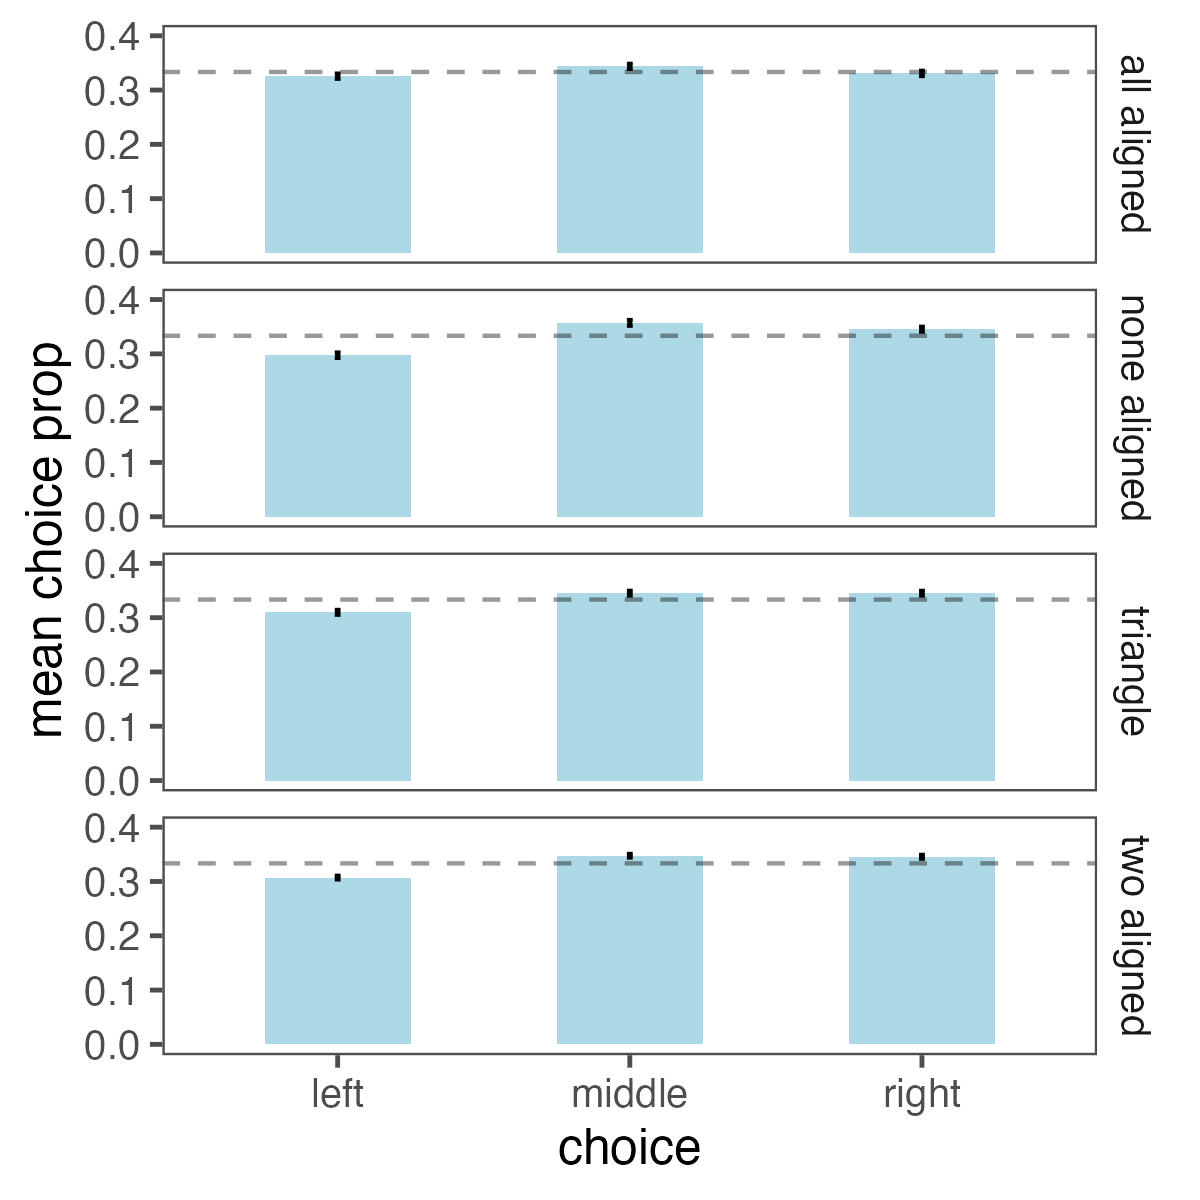
\includegraphics[width=100mm]{figures/comparability_filler_position_bias.jpeg}
   \caption{Position biases from non-critical trials in Experiment 5. Rows show trial types. Bars show mean proportion correct for a given position, with the error bars showing $\pm1\;\text{SEM}$. Dashed line is at chance ($1/3$).}
   \label{fig:comparability_pos_bias}
\end{figure}


\subsubsection{Critical Trials}

The goal of the critical trial analysis was to determine how alignment affected choice for a target option, defined as the rectangle located next to the decoy.

Consider the order of options on screen. There were six possible orderings: $DHW$, $DWH$, $HDW$, $HWD$, $WDH$, and $WHD$. Given that the crucial configuration is the two-aligned display, where the first two options are aligned vertically and a third option is unaligned both vertically and horizontally, the crucial trials are those trials where the decoy is among the first two options. 

The ordering was re-classified into a variable referred to as alignment. Because the two-aligned condition is the critical one, the the alignment variable is labeled based on the order in the two-aligned condition. If the ordering is $DHW$ or $HDW$, the alignment is "$H$ aligned with $D$". If the ordering is $WDH$ or $DWH$, the alignment is "$D$ aligned with $W$". The $WHD$ and $HWD$ trials were removed from further analysis but the results are included in the appendix.

The mean choice proportion for the $H$, $W$, and $D$ rectangles based on alignment were computed and are shown in Figure~\ref{fig:comparability_crit_mean_choices}. The data show that, in the two-aligned condition, participants were less likely to choose the $W$ option when it was aligned with $D$ than when $H$ was aligned with $D$. This effect also appears to occur in the none-aligned and all-aligned conditions, which suggests a position bias because choosing $H$ more when $W$ is aligned with $D$ but choosing $W$ more when $H$ is aligned with $D$ amounts to having a bias for the third (rightmost) rectangle.

\begin{figure}
   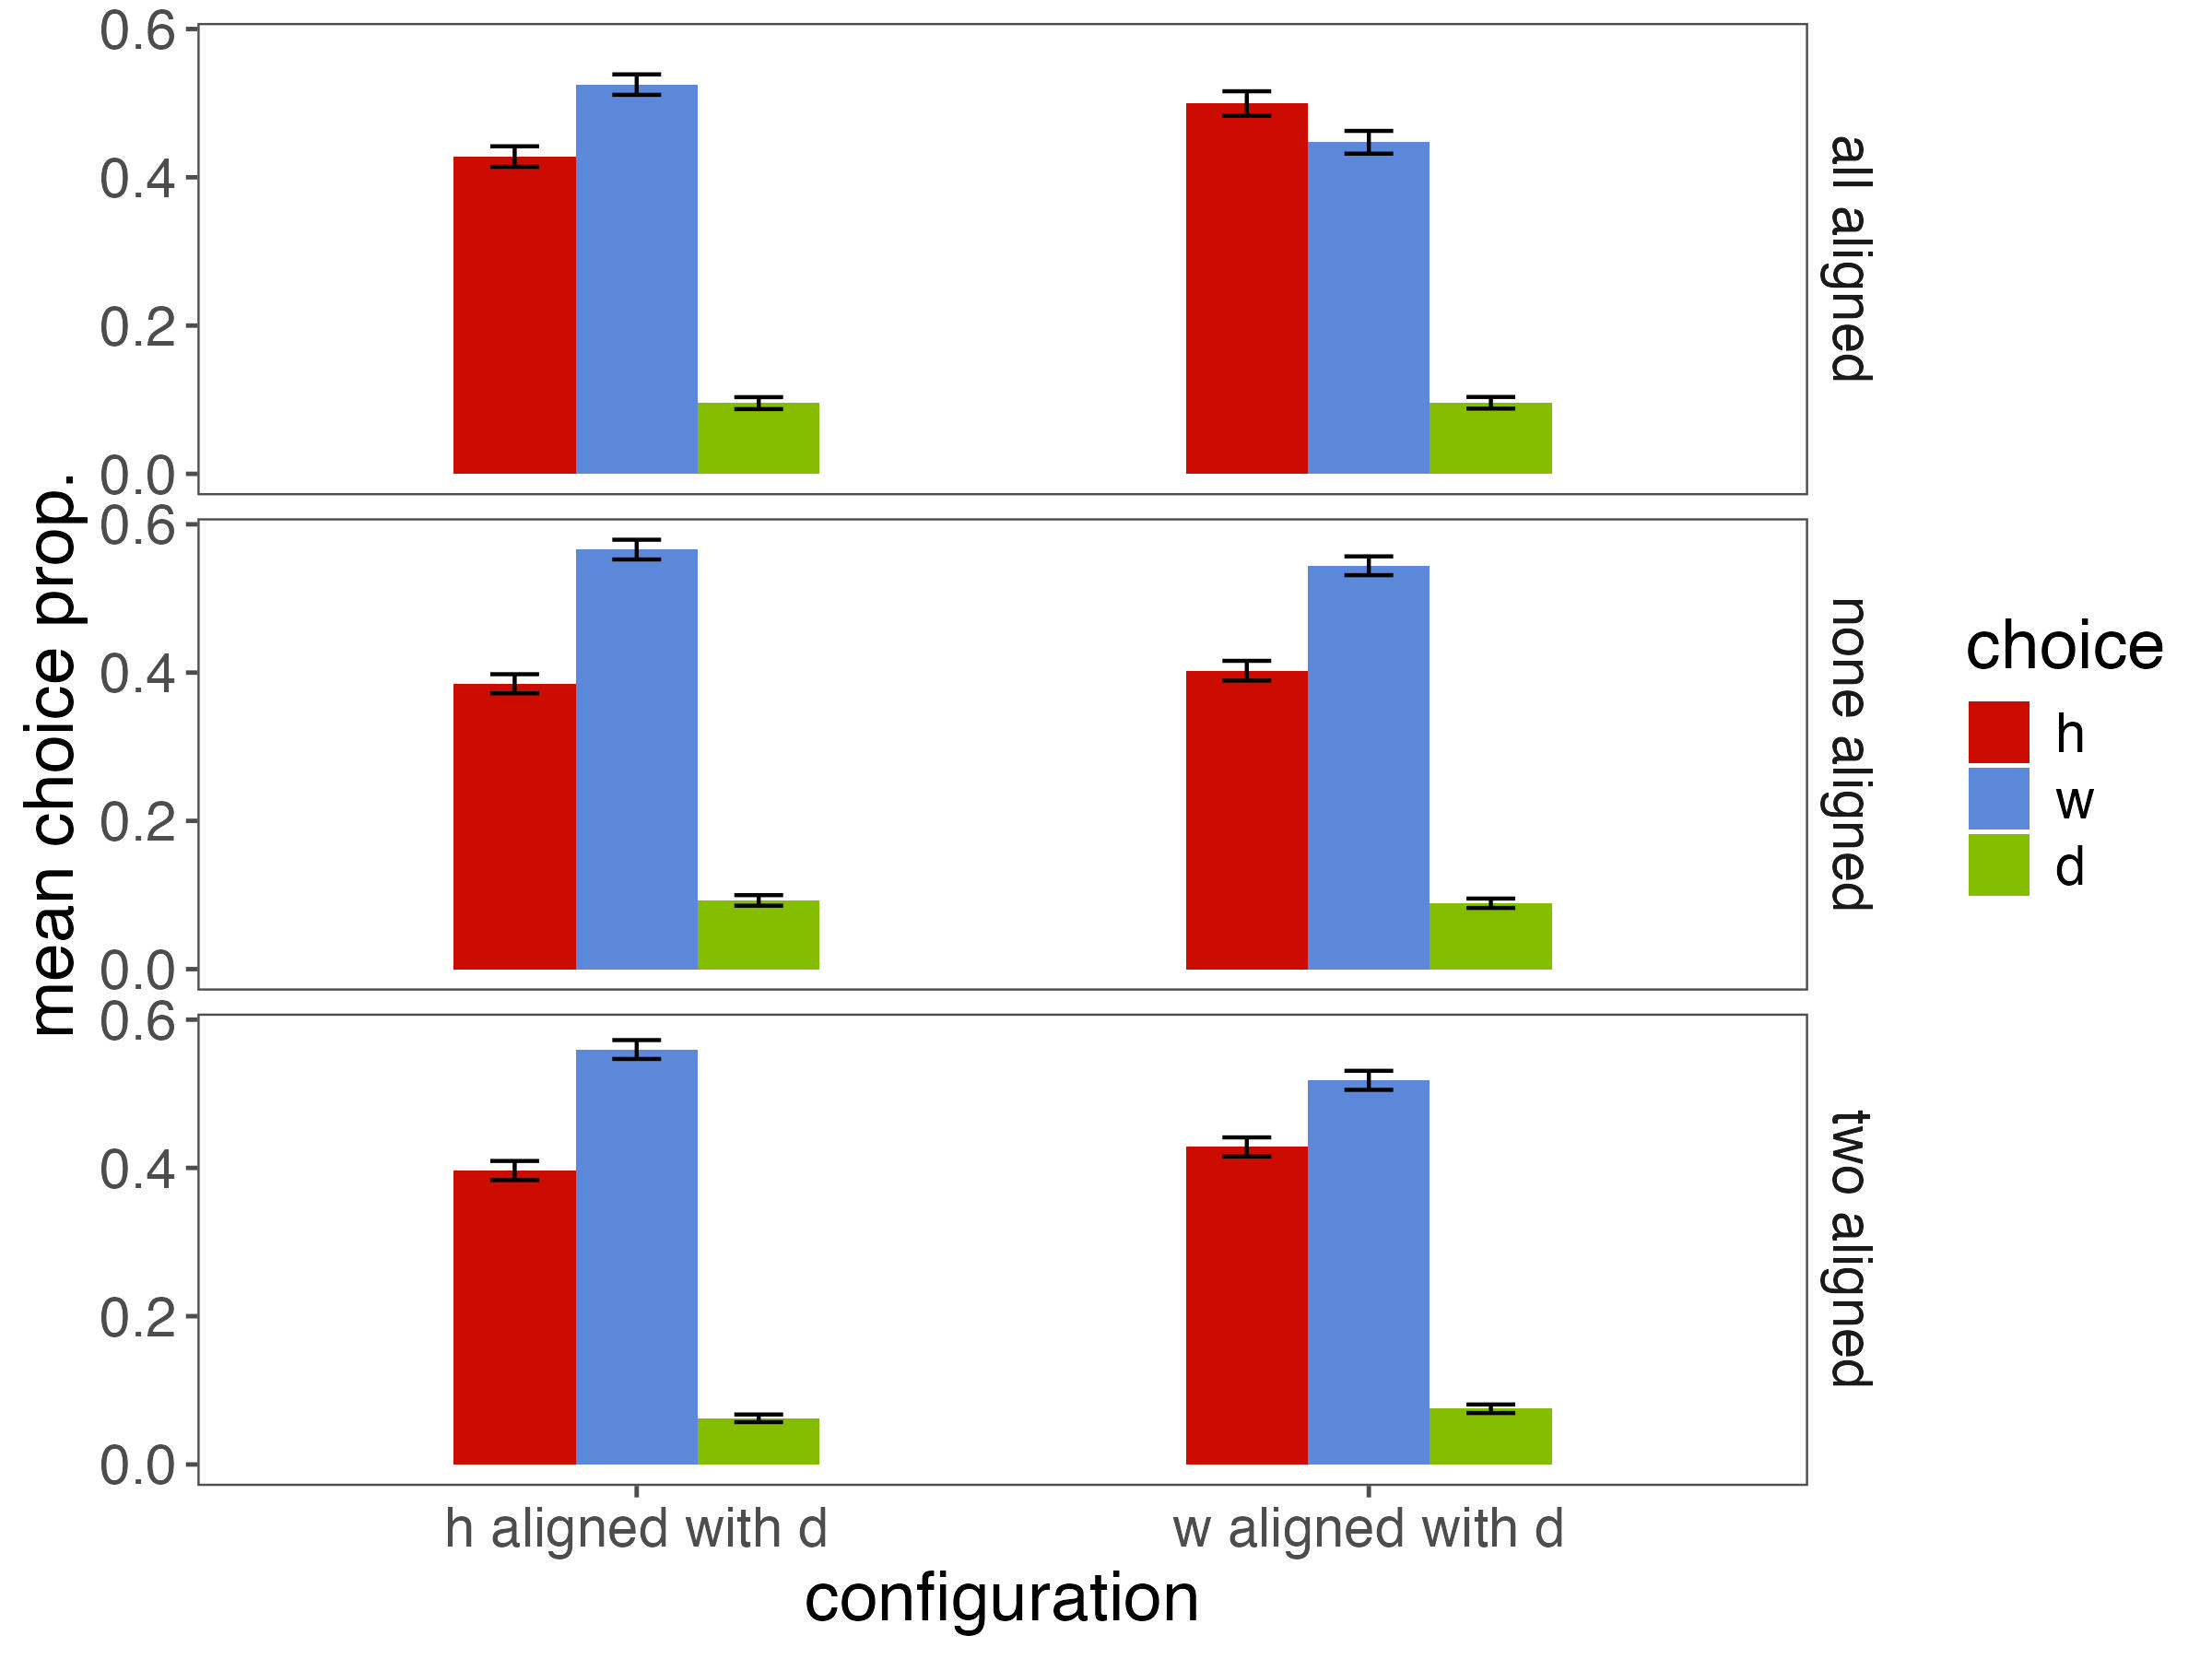
\includegraphics[width=100mm]{figures/comparability_crit_mean_hdw_choice_by_config_align.jpeg}
   \caption{Results from critical trials in Experiment 5. Mean choice proportions for the $H$, $W$, and $D$ rectangles conditioned on alignment and configuration. Error bars are $\pm1\mathrm{SEM}$.}
   \label{fig:comparability_crit_mean_choices}
\end{figure}

Next, the analyses were collapsed over $H$/$W$ and instead, choices were re-classified into target, competitor, and decoy. The target is the option aligned with the decoy, while the competitor is the option not aligned with the decoy. The decoy label did not change. Mean choice proportions were computed and plotted in Figure~\ref{fig:comparability_crit_mean_tcd_choices}.

Participants reliably chose the competitor more than the target; however, this effect appears to be stronger in the triangle condition, followed by the all aligned condition, the two aligned condition, and then the none aligned condition. Given that the triangle condition does not readily facilitate comparison between the decoy and the target, choosing the competitor more often in the triangle condition amounts to a bias for the third (rightmost) rectangle. A similar interpretation can be made for the none aligned condition. 

\begin{figure}
   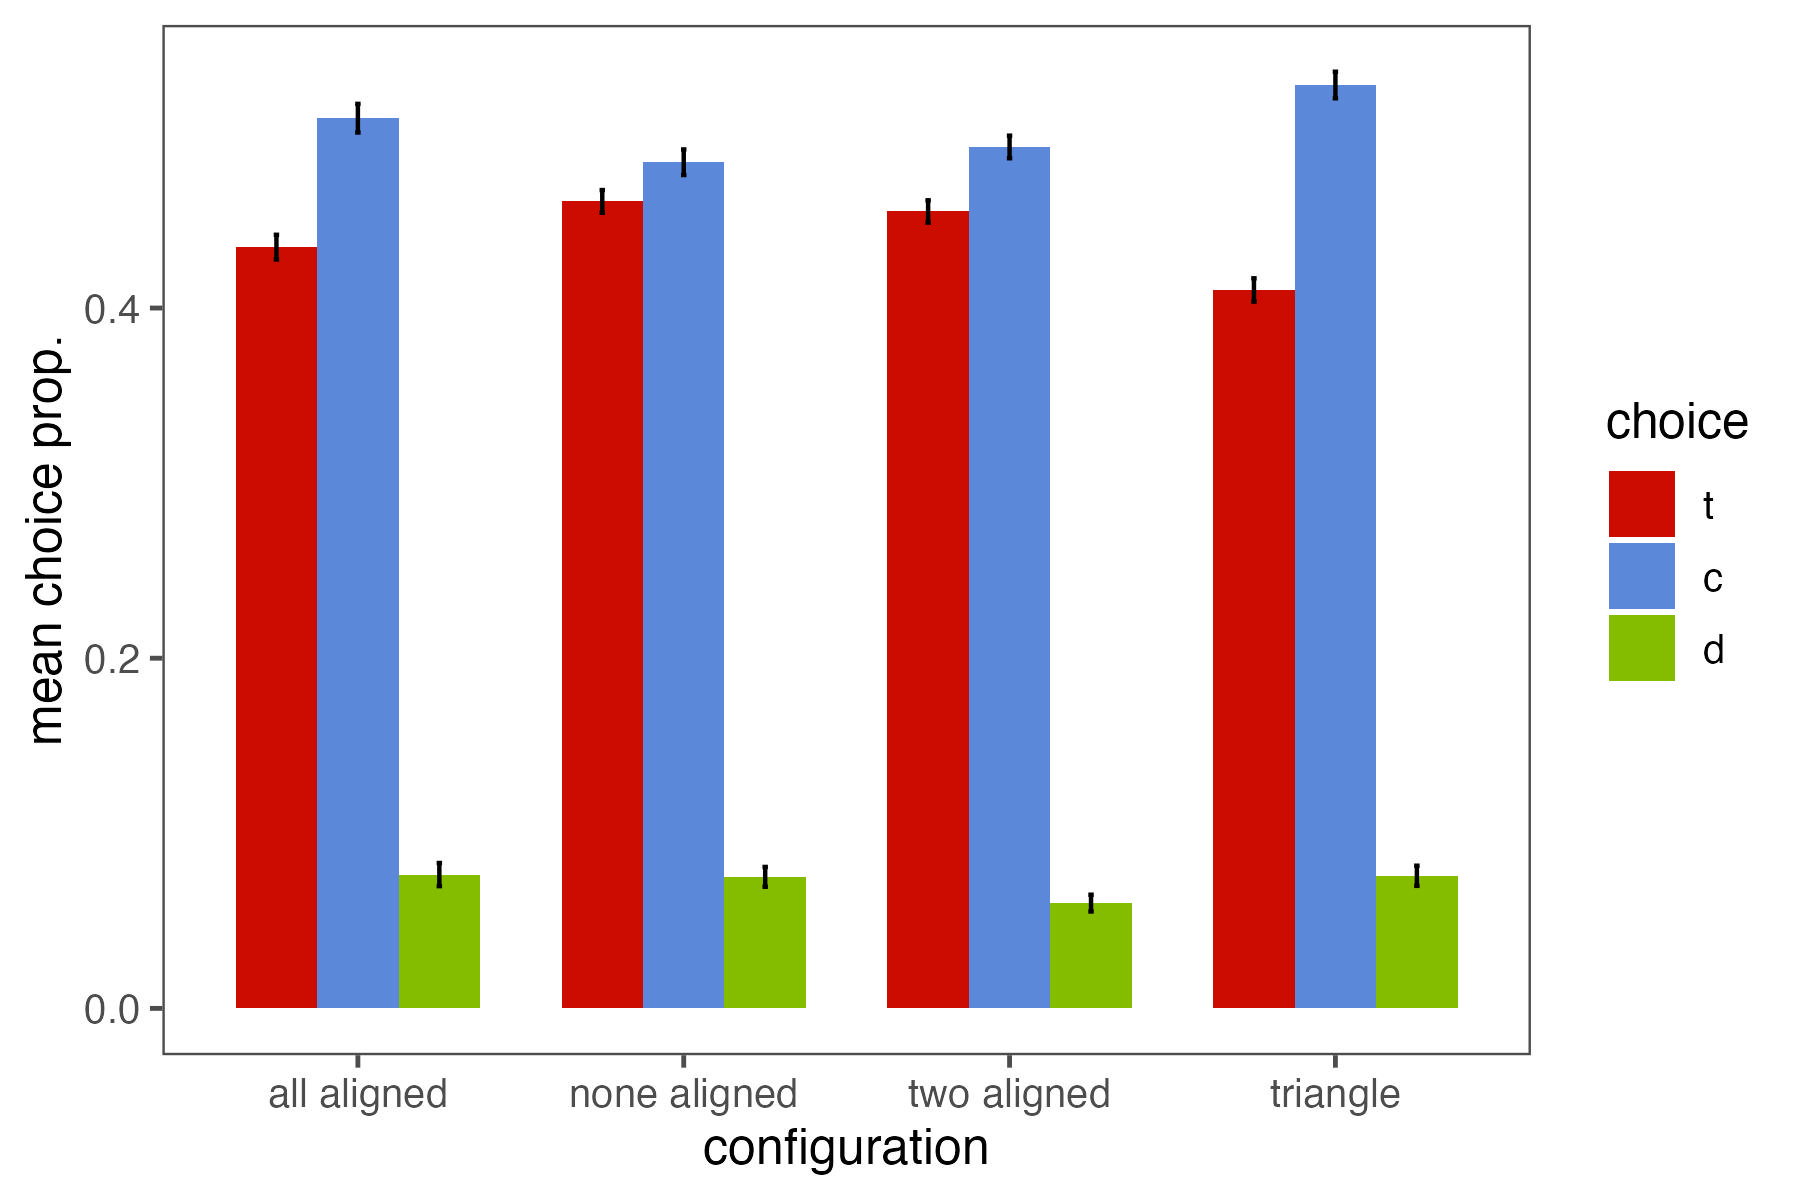
\includegraphics[width=100mm]{figures/comparability_crit_choice_by_config.jpeg}
   \caption{Experiment 5 mean target, competitor, and decoy choice proportions by configuration. Error bars are $\pm1\mathrm{SEM}$.}
   \label{fig:comparability_crit_mean_tcd_choices}
\end{figure}

Next, all trials in which participants chose the decoy were removed and Relative Share of the Target (RST) was computed. The mean RST is plotted in Figure~\ref{fig:comparability_crit_mean_target_choices}.

\begin{figure}
   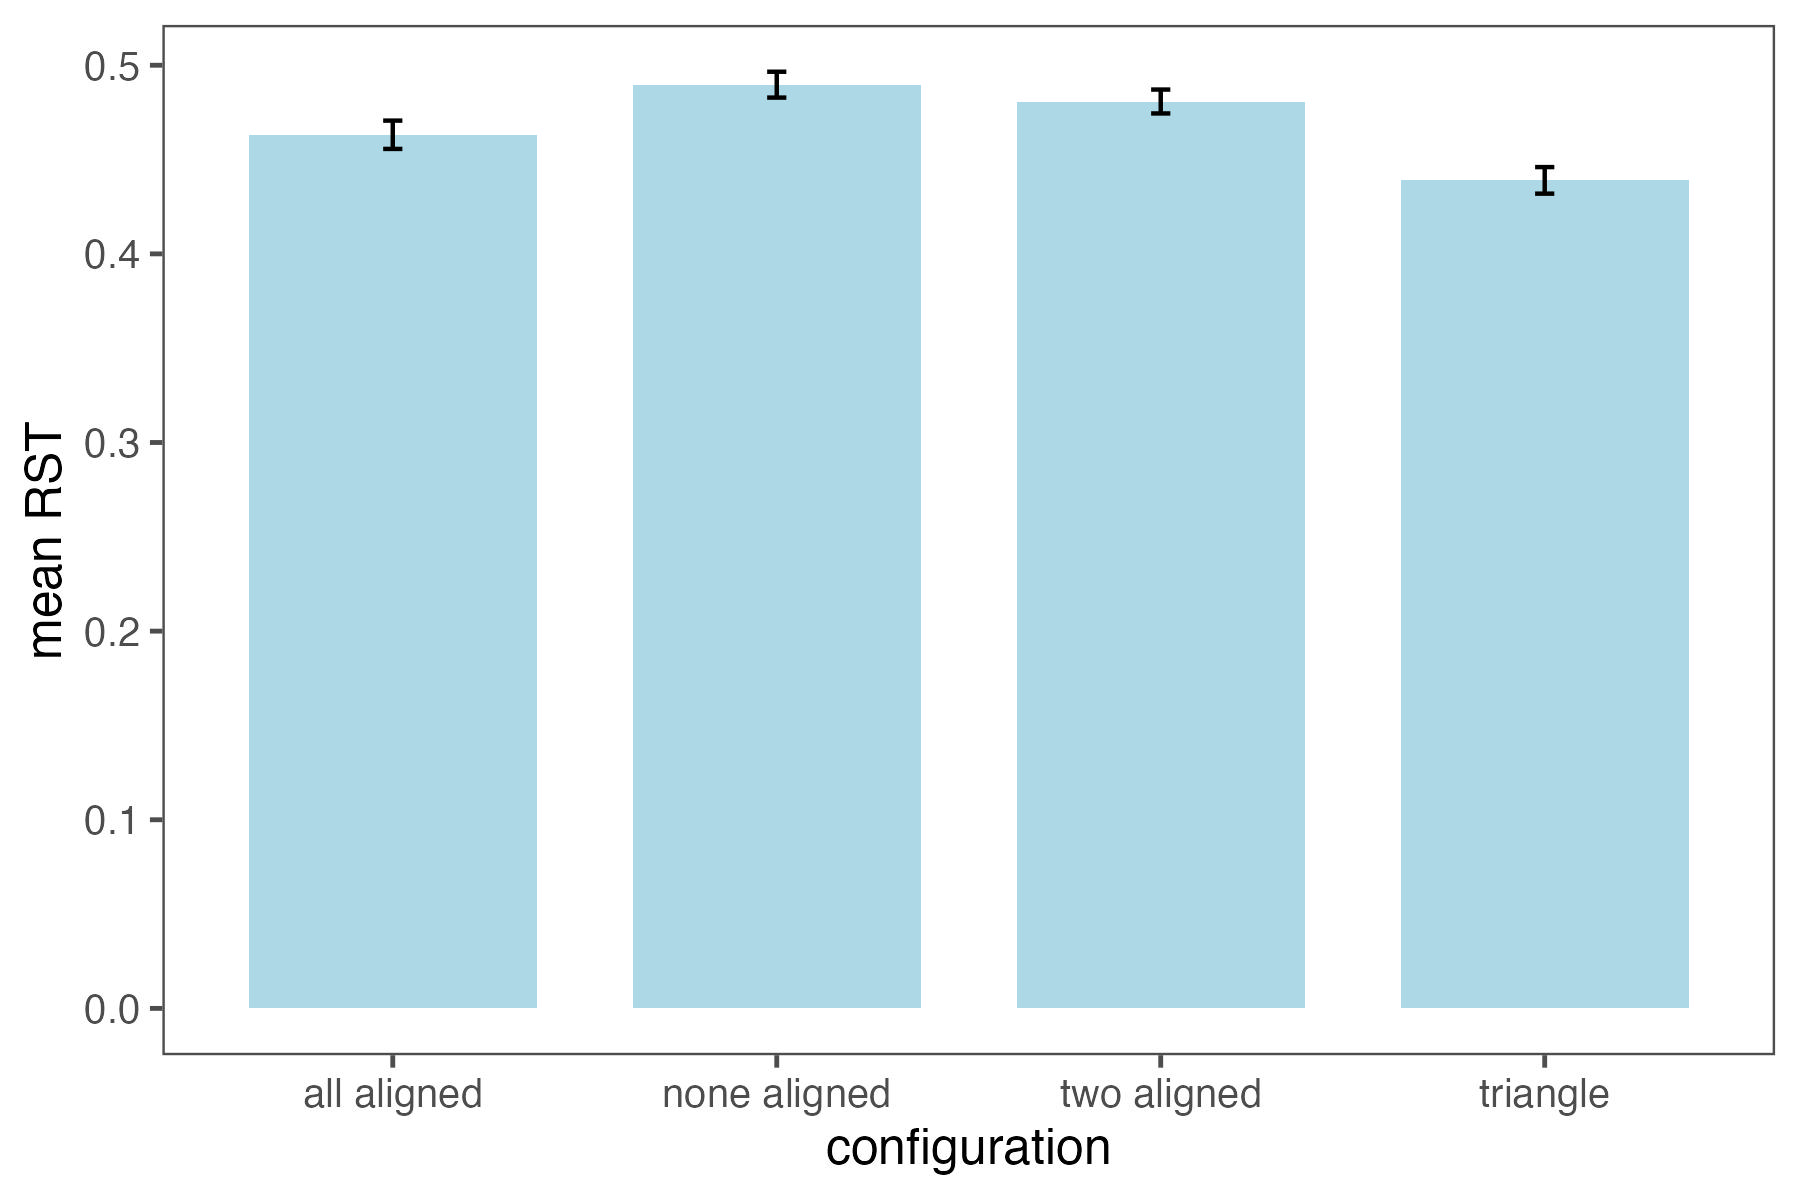
\includegraphics[width=100mm]{figures/comparability_crit_rst_by_config.jpeg}
   \caption{Experiment 5 mean RST by configuration. Error bars are $\pm1\mathrm{SEM}$.}
   \label{fig:comparability_crit_mean_target_choices}
\end{figure}

On average, participants select the target option on less than $1/2$ of trials (conditional on not having selected the decoy). This again may suggest a position bias; that is, participants appear to have a bias for the third (rightmost rectangle) in the choice set. However, crucially, they select the target less when it is aligned with the decoy in the two-aligned condition than when it is adjacent to the decoy in the none-aligned condition. See the Appendix for inferential statistics which support these conclusions, even after accounting for position bias and participant effects.

\section{Discussion}

Experiment 5 showed that comparability can affect choice. Given two equally viable dissimilar options, when one of these options (i.e., the target) was more easily comparable to a symmetrically dominated decoy option, participants chose the target less than the competitor. This effect is small but nonetheless present even after accounting for participant effects and a position bias.

This result aligns with the predictions from the Thurstonian perceptual choice model from Chapter 2. Increasing the comparability of a focal option and a decoy option increases the perceptual correlations between the two, which in turn decreases the choice share of the comparable \textit{target}, for the benefit of the non-comparable competitor option. This result is also similar to previous results presented by \textcite{trueblood2022attentional} and \textcite{evansImpactPresentationOrder2021}, who also manipulated the arrangement of options on screen in perceptual choice.

These results are, however, somewhat limited by the positioning of the target and decoy options. In the two-aligned conditon, the target and decoy were always presented in the first and second position. The statistical model accounted for this through a position bias effect, though a more thorough design would include a variety of presentation formats to more effectively test this effect.

Predictions were made assuming that increasing comparability decreased target choice share through perceptual correlation; however, given that these correlations were not measured directly, this may not be the case. It would be interesting to use the paradigm from Experiment 2 to directly measure the correlations between options when the decoy is symmetrically dominated and the comparability is systematically manipulated.

Future research should generalize this paradigm to high-level preferential choice. For example, given three consumer products, does the comparability of two of them affect the choice for a third option? For example, given three cars available for purchase, two of which are hybrids and the other is a traditional combustion engine vehicle, is the correlation between the hybrids stronger than the hybrid-combustion correlation? This question is left for future research.

When perceptual decisions are difficult, and a decoy option is easily comparable to one of two viable options, this viable option is chosen less than it otherwise would have been chosen. The effect was predicted using the Thurstonian model developed earlier in this dissertation, and the empirical result support it, albeit with limitations.  The empirical results of Experiment 5 demonstrate another form of context dependence, the main focus of this dissertation. Here, the context is not the choice set (which remains constant), but rather the presentation of the options. In this sense, the repulsion effect in this experiment is qualitatively similar to the repulsion effect of \textcite{spektorWhenGoodLooks2018b} and Experiment 2 of this dissertation.


\chapter{General Discussion and Conclusions}
\label{general_discussion_conclusion}
\section{General Discussion}

Decisions, even simple ones, may be impacted by context. Context effects occur when the relative choice for a particular option varies with situational properties. In particular, the set of other available affects choice. The attraction effect occurs when a decoy option boosts the choice share of a similar, superior target option. The repulsion effect, a reversal of the attraction effect, occurs when the decoy causes people to select the dissimilar competitor more than the target. 

This dissertation has explored context dependence in choice, largely by studying the attraction and repulsion effect (Chapters 2-4) but also through studying context dependence induced by the presentation format of options in simple perceptual choice (Chapter 5).

Chapter 2, a Thurstonian perceptual choice model was developed to measure the correlation between valuations in the attraction and repulsion effect. Experiment 1 demonstrated systematic discriminability issues in a 2AFC task in accordance with the Thurstonian model. In Experiment 2 participants provided both valuations (area judgments for rectanges) and choices (participants selected the largest rectangle from each ternary choice set). The model, conditional on parameters estimated from the judgment data, was used to make predictions for the choice data. When the $\rho_{TD}$ parameter is greater than both the $\rho_{TC}$ and $\rho_{CD}$ parameters, the Thurstonian model can parsimoniously account for the repulsion effect without invoking higher-level decision processes (Experiment 2). Conditional on the parameters the model cannot, however, account for the attraction effect, suggesting that higher-level decision processes may be required to explain this effect. 

In Chapter 3, the Thurstonian model was generalized to best-worst choice. In best-worst choice, participants select their most and least preferred options from a given choice set. Given the stimuli from Experiment 2 (a set of target, competitor, and decoy rectangles in a perceptual choice experiment), the model predicts a non-monotonic relationship between best and worst choice probabilities. Specifically, the model predicts that the target is both less likely to be chosen as worst, compared to the competitor, and also less likely to be chosen as best. This effect is not predicted by the maxdiff model, a highly influential of best-worst choice, which typically assumes independently distributed utilities. 

Chapter 4 generalized the paradigm and model from Chapter 2 to preferential choice. In Experiment 4, on each experimental trial, participants saw three consumer products (e.g., microwave ovens, laptops) and assigned each one a viable selling price. In later experimental trials, they saw the same three options and selected the option they most preferred. Data showed that the similarity, and comparability, of the target and decoy options, appears to generalize across choice types and can be reliably measured using Pearson correlations. The choice data also replicated previous researchers' choice results \parencite{banerjeeFactorsThatPromote2024}, albeit with limitations described in the text.

The model from Experiment 4 is able to qualitatively account for the repulsion effect, there is one crucial limitation here; the model accounts for the effect through the correlation between target and decoy evaluations, which causes the decoy to take choice shares away from the target. In preferential choice, and unlike perceptual choice, participants seldom if ever select the decoy. In the absence of these correlations, or if all correlations are equal (i.e., $\rho_{TD}=\rho_{TC}=\rho_{CD}$), the model will be unable to predict the effect\footnote{See the diagonal line from Figure~\ref{fig:3d_model} for evidence of this result.}. Thus, this form of the repulsion effect may be due to higher-level decision processes, or a hitherto unidentified low-level process. Nonetheless, the demonstration of target-decoy correlations, and indeed target-competitor correlations, is a novel result. 

Though other researchers have proposed correlations as a measure of the similarity between options in a choice set \parencite{kamakura1984predicting,natenzon2019random}, these studies was the first (to my knowledge) to systematically measure these correlations using valuations, incorporate them into a Thurstonian choice model, and connect this model to choices obtained from the same experimental participants.

Chapter 5 demonstrated a new form of context dependence, where choice systematically varies based on option comparability. In Chapter 5, Given a \textit{symmetrically dominated decoy} option, placing a focal target option in a nearby position, such that participants can more easily compare it to the decoy, \textit{decreased} the target's choice share. 

The results of this dissertation also have important methodological considerations. In particular researchers should carefully consider the assumptions made when designing and analyzing experiments. For example, the experiments of \textcite{spektorWhenGoodLooks2018b} contain a crucial assumption: that because participants chose the target more often the decoy, the repulsion effect observed in these experiments is a qualitative reversal of the attraction effect rather than just an empirical one. Chapter 3 showed that the independence assumption of the maxdiff choice model is incorrect (at least in some cases) and a failure to consider whether the stimuli of a given experiment can cause these violations may lead to incorrect conclusions about participants' preferences. The results of Chapter 5 show that the comparability, and even order on screen, can systematically affect choice. Previous researchers have also argued in favor of this point \parencite{trueblood2022attentional,hasan2025registered,evansImpactPresentationOrder2021}. 

There are numerous directions that this work could take beyond this dissertation. Future work could generalize the experimental and modeling paradigm of Experiment 2 to other context effects (e.g., compromise, similarity). Researchers should also correlations between option valuations at the individual participant level, which is currently limited by the quantity of data available. 

Regarding best-worst choice, future work should explore models of best-worst choice that can be used when the independence assumption is violated. Exploration, or development is necessary, is beyond the scope of this dissertation. However, given the numerous applied uses for best-worst choice, this avenue of research may improve researchers' ability to identify participants' preferences. 

Future work should also continue the line of research begun in Experiment 4. For example, research could collect both choice and pricing data from various binary and ternary sets. 

In addition to the experimental modifications discussed earlier, future work in comparability should generalize the paradigm to various choice types. Additionally, the effect observed in Experiment 5 was quite small; practically speaking, this may have limited impact on actual choices. Future work should address the limitations of comparability in affecting choice.

\section{Conclusions}
This dissertation has identified various forms of context dependence, in both perceptual and preferential choice. The research has provided theoretical explanations for these results in the form of a mathematical model of choice. To ensure falsifiability, The model's predictions were tested on out-of-sample data, to varying degrees of success. This work will further the study of context effects and decision-making in general. 

%% End of body
%%%%%%%%%%%%%%%%%%%%%%%%%%%%%%%%%%%%%%%%%%%%%%%%%%%%%%%%%%%%%%%%%%%%%%%%%%%%%%%

\appendix
\chapter{Bayesian Logistic Regression Model of 2AFC Discriminability from Experiment 1}
I analyzed the 2AFC data from Experiment 1 using Bayesian Hierarchical Logistic Regression. 

Recall that in this experiment, participants were presented with three stimuli (target, competitor, and decoy rectangles). They were then asked to select the largest rectangle out of a pair of two of these options. In other words, there are three trial types: target/competitor (TC), target/decoy (TD), and competitor/decoy (CD). As discussed in the main text, I remove the TC trials from all substantive analyses, as well as the $TDD=0\%$ trials. 

\section{Model Details} 

The model predicts the probability of discriminating the target/competitor from the decoy option. According to the model, discrimination $D$ for participant $i$ on trial $j$ is:
\begin{align}
    D_{ij} \sim Bernoulli(\theta_{ij})
\end{align}

To compute $\theta_{ij}$, I first compute $\eta_{ij}$ from linear combination of the relevant variables.

\begin{equation}
    \begin{aligned}
        \eta_{ij} &= (\beta_{0} + S_{0_{i}}) + (\beta_{\mathrm{or}} + S_{\mathrm{or}_{i}}) \cdot \mathrm{or}_{ij} + (\beta_{\mathrm{horiz}} + S_{\mathrm{horiz}_{i}}) \cdot \mathrm{horiz}_{ij} \\
        &\quad + (\beta_{\mathrm{TD}} + S_{\mathrm{TD}_{i}}) \cdot \mathrm{TD}_{ij} + (\beta_{\mathrm{TDD5}} + S_{\mathrm{TDD5}_{i}}) \cdot \mathrm{TDD5}_{ij} + (\beta_{\mathrm{TDD9}} + S_{\mathrm{TDD9}_{i}}) \cdot \mathrm{TDD9}_{ij} \\
        &\quad + (\beta_{\mathrm{TDD14}} + S_{\mathrm{TDD14}_{i}}) \cdot \mathrm{TDD14}_{ij} + (\beta_{\mathrm{TDD5xTD}} + S_{\mathrm{TDD5xTD}_{i}}) \cdot \mathrm{TDD5}_{ij} \cdot \mathrm{TD}_{ij} \\
        &\quad + (\beta_{\mathrm{TDD9xTD}} + S_{\mathrm{TDD9xTD}_{i}}) \cdot \mathrm{TDD9}_{ij} \cdot \mathrm{TD}_{ij} + (\beta_{\mathrm{TDD14xTD}} + S_{\mathrm{TDD14xTD}_{i}}) \cdot \mathrm{TDD14}_{ij} \cdot \mathrm{TD}_{ij}
    \end{aligned}
\end{equation}

All $\beta$ terms are fixed effects, and all $S$ terms are random (participant) effects. $\beta_{or}$ is the fixed effect of orientation, where $\text{or}_{ij}$ is a dummy variable which $=0$ if the target and decoy are taller than wide and $=1$ if the target and decoy are wider than tall. $\beta_{TD}$ is the fixed effect of comparison, where $TD_{ij}$=0 for CD trials and $TD_{ij}=1$ for TD trials.  The $TDD$ variable has 4 levels ($2\%$, $5\%$, $9\%$, and $14\%$), so I include three dummy variables ($TDD5$, $TDD9$, and $TDD14$) and treat $2\%$ as the reference level for $TDD$. I also include the interaction to capture the additional boost / decrement to $TD$ over $TC$ trials at each level of $TDD$. 

$\eta_{ij}$ is then transformed to the probability scale using the logit function:

\begin{align}
    \theta_{ij}=\frac{1}{1+e^{-\eta_{ij}}}
\end{align}

\section{Prior Distributions on Parameters}

\begin{itemize}
    \item $\beta_{0} \sim \mathcal{N}(0,5)$
    \item $\beta_{or} \sim \mathcal{N}(0,5)$
    \item $\beta_{horiz} \sim \mathcal{N}(0,5)$
    \item $\beta_{TD} \sim \mathcal{N}(0,5)$
    \item $\beta_{TDD5} \sim \mathcal{N}(0,5)$
    \item $\beta_{TDD9} \sim \mathcal{N}(0,5)$
    \item $\beta_{TDD14} \sim \mathcal{N}(0,5)$
    \item $\beta_{TDD5xTD} \sim \mathcal{N}(0,2.5)$
    \item $\beta_{TDD9xTD} \sim \mathcal{N}(0,2.5)$
    \item $\beta_{TDD14xTD} \sim \mathcal{N}(0,2.5)$
    \item $S_{0_{i}} \sim \mathcal{N}(0, \sigma_{S_0})$
    \item $S_{or_{i}} \sim \mathcal{N}(0, \sigma_{S})$
    \item $S_{horiz_{i}} \sim \mathcal{N}(0, \sigma_{S})$
    \item $S_{TD_{i}} \sim \mathcal{N}(0, \sigma_{S})$
    \item $S_{TDD5_{i}} \sim \mathcal{N}(0, \sigma_{S})$
    \item $S_{TDD9_{i}} \sim \mathcal{N}(0, \sigma_{S})$
    \item $S_{TDD14_{i}} \sim \mathcal{N}(0, \sigma_{S})$
    \item $S_{TDD5xTD_{i}} \sim \mathcal{N}(0, \sigma_{S})$
    \item $S_{TDD9xTD_{i}} \sim \mathcal{N}(0, \sigma_{S})$
    \item $S_{TDD14xTD_{i}} \sim \mathcal{N}(0, \sigma_{S})$
    \item $\sigma_{S_{0}} \sim \text{LogNormal}(0,2.5)$
    \item $\sigma_{S} \sim \text{LogNormal}(0,2.5)$
\end{itemize}

Note that the model assumes equal variance for all random effect distributions aside from the random intercepts.

\section{Modeling Results}
The model was coded in Stan \parencite{carpenter2017stan} and implemented using the RStan package \parencite{rstan}. The sampler ran $5$ chains, each for $2500$ iterations. Posterior diagnostics indicated that the sampler converged.

\subsection{Parameter estimates.}

Table~\ref{tab:e1_params} shows parameter estimates, including means and $95\%$ credible intervals. 
\begin{table}[ht]
    \centering
    \begin{tabular}{lrrrr}
        \toprule
        Parameter & M & SD & CI low & CI high \\
        \midrule
        $\beta_{0}$ & 0.44 & 0.06 & 0.32 & 0.57 \\
        $\beta_{or}$ & -0.54 & 0.06 & -0.66 & -0.43\\
        $\beta_{horiz}$ & 0.23 & 0.06 & 0.12 & 0.34\\
        $\beta_{TD}$ & 0.17 & 0.08 & 0.01 & 0.33\\
        $\beta_{TDD5}$ & 0.40 & 0.08 & 0.23 & 0.56\\
        $\beta_{TDD9}$ & 0.81 & 0.09 & 0.64 & 0.98\\
        $\beta_{TDD14}$ & 1.45 & 0.10 & 1.25 & 1.64\\
        $\beta_{TDD5xTD}$ & 0.14 & 0.12 & -0.09 & 0.36\\
        $\beta_{TDD9xTD}$ & 0.61 & 0.13 & 0.36 & 0.85\\
        $\beta_{TDD14xTD}$ & 0.79 & 0.15 & 0.50 & 1.10\\
        $\sigma_{S_0}$ & 0.20 & 0.04 & 0.12 & 0.29 \\
        $\sigma_{S}$ & 0.34 & 0.03 & 0.29 & 0.39 \\
    \bottomrule 
    \end{tabular}
    \caption{Parameter estimates for Bayesian Hierarchical Logistic Regression from Experiment 1 Data, including means, standard deviations, and $95\%$ Credible Intervals.}
    \label{tab:e1_params}
 \end{table}
    
 Inference is made by examining the posterior distributions of the fixed effect parameters (i.e., all $\beta$ values). 

\chapter{Bayesian Hierarchical Modeling of Circle Estimation Data from Experiment 2}

I analyzed the circle estimation data (Experiment 2) using the multivariate Thurstonian perceptual model first presented in Chapter 2. 

\section{Model Details}

The model assumes that, for participant $i$ on trial $j$, the vector of perceived areas $\boldsymbol{X}_{ij}$ is sampled from a multivariate normal distribution with parameters $\boldsymbol{\mu}_{ij}$ and $\boldsymbol{\Sigma}$. That is,
\begin{align}
    \boldsymbol{X}_{ij} \sim \mathcal{N}(\boldsymbol{\mu}_{ij},\boldsymbol{\Sigma})
\end{align}

Using Bayesian statistical modeling, I simultaneously estimated the parameters  $\boldsymbol{\mu}$ and $\boldsymbol{\Sigma}$ for the model outlined in Chapter 2. Note that I allow $\boldsymbol{\mu}$ to vary systematically over trials and participants, but $\Sigma$ remains constant. I estimate $\boldsymbol{\mu}$ using hierarchical regression while allowing the components of $\boldsymbol{\Sigma}$ (i.e., $\boldsymbol{\sigma_{T}}$, $\boldsymbol{\sigma_{C}}$, $\boldsymbol{\sigma_{D}}$, $\rho_{TD}$, $\rho_{TC}$, $\rho_{CD}$) to vary freely. 

I estimated the model separately for the triangle and horizontal condition. I first walk through the computation of $\boldsymbol{\mu}$, followed by the computation $\boldsymbol{\Sigma}$. I also show the prior distributions on each parameter separately for each of these components, and then I explain the modeling procedure and results. Note that the model predicts mean-centered log-transformed estimated area.

\subsection{\texorpdfstring{$\boldsymbol{\mu}$}{mu} Parameterization}

I used the model to predict the mean area $\mu_{ijk}$ for the $i$th participant on the $j$th trial for the $k$th stimulus. There were $k=3$ stimuli on each trial. If $k=1$, the stimulus is the target; If $k=2$, the stimulus is the competitor; If $k=3$, the stimulus is the decoy. Thus, $\boldsymbol{\mu}$ can be broken down into $\mu_{ij1}$ (target), $\mu_{ij2}$ (competitor), and $\mu_{ij3}$ (decoy). Note that some parameters are common to all stimuli (e.g., the effects of diagonal or orientation), while others are common only to a particular option (e.g., the effect of competitor vs. decoy vs. target). 

$\mu_{ij1}$ is computed as:

\begin{equation}
    \begin{aligned}
        \mu_{ij3}=(S_{0_i} + \beta_{0}) + \beta_{or}*\mathrm{or}_{ij1} + \beta_{\mathrm{diag}2}*\mathrm{diag}2_{ij}+ \\
        \beta_{\mathrm{diag}3}*\mathrm{diag}3_{ij} + \beta_{\mathrm{TDD}5}*\mathrm{TDD}5_{ij} +\\ \beta_{\mathrm{TDD}9}*\mathrm{TDD}9_{ij} + \beta_{\mathrm{TDD}14}*\mathrm{TDD}14_{ij}
        \label{circle_mu_eqn1}
    \end{aligned}
\end{equation}

$S_{0_i}$ is a random intercept for participant $i$. $\beta_{0}$ is the fixed intercept. $\beta_{or}$ is the fixed effect of orientation, where $or_{ij1}$ is a dummy variable which $=0$ if the target is taller than wide and $=1$ if the target is wider than tall. $\beta_{diag2}$ is the fixed effect of the middle diagonal, which $=1$ if the all stimuli on the trial fall on the middle diagonal and $=0$ otherwise. $\beta_{diag3}$ is the fixed effect of the upper diagonal, which $=1$ if all stimuli on the trial fall on the upper diagonal and $=0$ otherwise. $\beta_{TDD5}$ is the fixed effect of TDD 5, and $TDD5_{ij}$ is a dummy variable which $=1$ if $TDD=5\%$ and $=0$ otherwise. $\beta_{TDD9}$ is the fixed effect of TDD 9, and $TDD9_{ij}$ is a dummy variable which $=1$ if $TDD=9\%$ and $=0$ otherwise. $\beta_{TDD14}$ is the fixed effect of TDD 14, and $TDD14_{ij}$ is a dummy variable which $=1$ if $TDD=14\%$ and $=0$ otherwise. 

$\mu_{ij2}$ is computed as:

\begin{equation}
    \begin{aligned}
        \mu_{ij2}=(S_{0_i} + \beta_{0}) + \beta_{\mathrm{or}}*\mathrm{or}_{ij2} + \beta_{\mathrm{diag}2}*\mathrm{diag}2_{ij}+ \\\beta_{\mathrm{diag}3}*\mathrm{diag}3_{ij} + \beta_{\mathrm{TDD}5}*\mathrm{TDD}5_{ij} + \\\beta_{\mathrm{TDD}9}*\mathrm{TDD}9_{ij} + \beta_{\mathrm{TDD}14}*\mathrm{TDD}14_{ij} + \beta_{\mathrm{comp}}
        \label{circle_mu_eqn2}
    \end{aligned}
\end{equation}

$S_{0_i}$ is a random intercept for participant $i$. $\beta_{0}$ is the fixed intercept. $\beta_{or}$ is the fixed effect of orientation, where $or_{ij2}$ is a dummy variable which $=0$ if the competitor is taller than wide and $=1$ if the competitor is wider than tall. $\beta_{diag2}$ is the fixed effect of the middle diagonal, which $=1$ if the all stimuli on the trial fall on the middle diagonal and $=0$ otherwise. $\beta_{diag3}$ is the fixed effect of the upper diagonal, which $=1$ if all stimuli on the trial fall on the upper diagonal and $=0$ otherwise. $\beta_{TDD5}$ is the fixed effect of TDD 5, and $TDD5_{ij}$ is a dummy variable which $=1$ if $TDD=5\%$ and $=0$ otherwise. $\beta_{TDD9}$ is the fixed effect of TDD 9, and $TDD9_{ij}$ is a dummy variable which $=1$ if $TDD=9\%$ and $=0$ otherwise. $\beta_{TDD14}$ is the fixed effect of TDD 14, and $TDD14_{ij}$ is a dummy variable which $=1$ if $TDD=14\%$ and $=0$ otherwise. $\beta_{comp}$ is a parameter that reflects the possibility of estimation bias for the competitor.

$\mu_{ij3}$ is computed as:

\begin{equation}
    \begin{aligned}
        \mu_{ij3}=(S_{0_i} + \beta_{0}) + \beta_{\mathrm{or}}*\mathrm{or}_{ij3} + \beta_{\mathrm{diag}2}*\mathrm{diag}2_{ij}+ \\\beta_{\mathrm{diag}3}*\mathrm{diag}3_{ij} + (\beta_{\mathrm{TDD}5} + \beta_{\mathrm{TDD}5D})*\mathrm{TDD}5D_{ij} + (\beta_{\mathrm{TDD}9} + \beta_{\mathrm{TDD}9D})*\mathrm{TDD}9D_{ij} +\\ (\beta_{\mathrm{TDD}14} +\\ \beta_{\mathrm{TDD}14D})*\mathrm{TDD}14D_{ij}
        \label{circle_mu_eqn3}
    \end{aligned}
\end{equation}

$S_{0_i}$ is a random intercept for participant $i$. $\beta_{0}$ is the fixed intercept. $\beta_{or}$ is the fixed effect of orientation, where $or_{ij3}$ is a dummy variable which $=0$ if the decoy is taller than wide and $=1$ if the decoy is wider than tall. $\beta_{diag2}$ is the fixed effect of the middle diagonal, which $=1$ if the all stimuli on the trial fall on the middle diagonal and $=0$ otherwise. $\beta_{diag3}$ is the fixed effect of the upper diagonal, which $=1$ if all stimuli on the trial fall on the upper diagonal and $=0$ otherwise. $\beta_{TDD5D}$ is the fixed effect of TDD=5, and $TDD5D_{ij}$ is a dummy variable which $=1$ if $TDD=5\%$ for the decoy and $=0$ otherwise. $\beta_{TDD9D}$ is the fixed effect of TDD 9 for the decoy, and $TDD9D_{ij}$ is a dummy variable which $=1$ if $TDD=9\%$ and $=0$ otherwise. $\beta_{TDD14D}$ is the fixed effect of TDD 14 for the decoy, and $TDD14D_{ij}$ is a dummy variable which $=1$ if $TDD=14\%$ and $=0$ otherwise. 

Note that there is a common set of parameters for each level of TDD and additional set of parameters for each level of TDD that only apply to the decoy. In the data, it was clear that participants often adjusted the target and competitor relative to the decoy. In other words, even though the physical size of both target and competitor remains constant across TDD, participants' \textit{estimation} of their size varied with TDD. The inclusion of a separate set of parameters for TDD that only apply to the decoy allows for a "deflection" of the decoy size, relative to target and competitor size. 

Note the following reference points for the variables:
\begin{itemize}
    \item TDD: $2\%$
    \item Orientation: taller than wide
    \item Diagonal: lower
    \item Stimulus: target
\end{itemize}

The $\beta_{0}$ parameter captures the fixed of a tall target on the lower diagonal at $2\%$ TDD, and all other parameters reflect deflections from this.

\subsubsection{Prior Distributions on Parameters}
Below are shown the following prior distributions on each parameter relevant to $\boldsymbol{\mu}$:
\begin{itemize}
    \item $\beta_{0} \sim \mathcal{N}(0,5)$
    \item $\beta_{or} \sim \mathcal{N}(0,5)$
    \item $\beta_{diag2} \sim \mathcal{N}(0,5)$
    \item $\beta_{diag3} \sim \mathcal{N}(0,5)$
    \item $\beta_{TDD5} \sim \mathcal{N}(0,5)$
    \item $\beta_{TDD9} \sim \mathcal{N}(0,5)$
    \item $\beta_{TDD14} \sim \mathcal{N}(0,5)$
    \item $\beta_{TDD2D} \sim \mathcal{N}(0,5)$
    \item $\beta_{TDD5D} \sim \mathcal{N}(0,5)$
    \item $\beta_{TDD9D} \sim \mathcal{N}(0,5)$
    \item $\beta_{TDD14D} \sim \mathcal{N}(0,5)$
    \item $\beta_{comp} \sim \mathcal{N}(0,5)$
    \item $S_{0_i} \sim \mathcal{N}(0,\sigma_{S_0})$
    \item $\sigma_{S_0} \sim \text{Half-Cauchy}(0, 2.5)$
\end{itemize}

\section{$\boldsymbol{\Sigma}$ Parameterization}
$\Sigma$ is a positive semi-definite $3\text{x}3$ covariance matrix computed as:

\begin{align}
   \boldsymbol{\Sigma}=S\boldsymbol{\Omega}S
   \label{eqn:Sigma}
\end{align}

where $S$ is a diagonal matrix consisting of: 

\begin{align}
   \begin{pmatrix}
      \sigma_{T} & 0 & 0 \\
      0 & \sigma_{C} & 0 \\
      0 & 0 & \sigma_{D} \\
   \end{pmatrix}
   \label{eqn:S}
\end{align}

and $\boldsymbol{\Omega}$ is a correlation matrix:

\begin{align}
   \begin{pmatrix}
      1 & \rho_{TC} & \rho_{TD} \\
      \rho_{TC} & 1 & \rho_{CD} \\
      \rho_{TD} & \rho_{CD} & 1 \\
   \end{pmatrix}
   \label{eqn:O}
\end{align}

Estimation of $S$ was straightforward. I simply freely estimated the three standard deviation parameters $\sigma_{T}$, $\sigma_{C}$, and $\sigma_{D}$.

To estimate $\boldsymbol{\Omega}$, I used the LKJ distribution \parencite{lewandowski2009generating} to set priors on the Cholesky factorization of the correlation matrix $\Omega$. This was done to ensure that the resulting variance-covariance matrix $\boldsymbol{\Sigma}$ is positive semi-definite, a requirement of the multivariate Gaussian distribution. The critical inferences, however, are performed on the off-diagonal elements $\rho_{TC}$, $\rho_{TD}$, $\rho_{CD}$ in each display condition. I set priors on the $\sigma$ parameters using the Half-Cauchy distribution \parencite{gelman2006prior}. 

\subsubsection{Prior Distributions on Parameters}
Below are shown the following prior distributions on each parameter relevant to $\boldsymbol{\Sigma}$.
\begin{itemize}
    \item $\sigma_{T} \sim\text{Half-Cauchy}(0,2.5)$
    \item $\sigma_{C} \sim\text{Half-Cauchy}(0,2.5)$
    \item $\sigma_{D} \sim\text{Half-Cauchy}(0,2.5)$
    \item $\boldsymbol{\Omega} \sim \text{LKJCorr}(\eta=1)$
\end{itemize}

\section{Modeling Results}
The model was implemented using the Stan programming language \parencite{carpenter2017stan} using the cmdstanr interface \parencite{cmdstanr} in R . 

I ran the model for 2500 iterations (not including warm-up) with 4 chains for each display condition. Posterior diagnostics indicated that the sampler converged in each condition.

Below I show parameter estimates for each display condition and relevant parameter. I exclude the estimates of the participant effects $S_{0_i}$ for brevity. Estimates are rounded to two or three decimal places, depending on the size of the parameter.
    
\begin{table}[ht]
    \centering
    \begin{tabular}{llrrrr}
        \toprule
        Display Condition & Parameter & \textit{M} & \textit{SD} & HDI lower & HDI upper \\
        \midrule
        \textbf{Horizontal}  &  $\beta_{0}$     &    $-0.41$   &   $0.02$    &  $-0.44$     & $-0.38$     \\
                    &  $\beta_{or}$    &    $0.003$   &   $0.002$   &  $-0.001$    & $0.007$     \\
                    &  $\beta_{diag2}$ &    $0.47$    &   $0.01$    &  $0.46$      & $0.48$      \\
                    &  $\beta_{diag3}$ &    $0.80$    &   $0.01$    &  $0.79$      & $0.81$      \\
                    &  $\beta_{TDD5}$  &    $-0.005$  &   $0.01$    &  $-0.017$    & $0.007$     \\
                    &  $\beta_{TDD9}$  &    $-0.007$  &   $0.01$    &  $-0.019$    & $0.005$     \\
                    &  $\beta_{TDD14}$ &    $-0.01$   &   $0.01$    &  $-0.02$     & $-0.0005$   \\
                    &  $\beta_{TDD2D}$ &    $-0.006$  &   $0.004$   &  $-0.013$    & $0.001$     \\
                    &  $\beta_{TDD5D}$ &    $-0.01$   &   $0.004$   &  $-0.016$    & $-0.003$    \\
                    &  $\beta_{TDD9D}$ &    $-0.04$   &   $0.004$   &  $-0.05$     & $-0.04$     \\
                    &  $\beta_{TDD14D}$&    $-0.08$   &   $0.004$   &  $-0.09$     & $-0.07$     \\
                    &  $\beta_{comp}$  &    $0.003$   &   $0.002$   &  $-0.002$    & $0.007$     \\
                    &  $\sigma_{S_0}$  &    $0.19$    &   $0.01$    &  $0.17$      & $0.21$      \\
                    &  $\sigma_{T}$    &    $0.337$   &   $0.002$   &  $0.334$     & $0.340$     \\
                    &  $\sigma_{C}$    &    $0.341$   &   $0.002$   &  $0.338$     & $0.345$     \\
                    &  $\sigma_{D}$    &    $0.337$   &   $0.002$   &  $0.333$     & $0.340$     \\
                    &  $\rho_{TC}$     &    $0.575$   &   $0.005$   &  $0.565$     & $0.584$     \\
                    &  $\rho_{TD}$     &    $0.710$   &   $0.004$   &  $0.703$     & $0.716$     \\
                    &  $\rho_{CD}$     &    $0.575$   &   $0.005$   &  $0.565$     & $0.584$     \\
        \textbf{Triangle}    &  $\beta_{0}$     &    $-0.40$   &   $0.01$    &  $-0.42$     & $-0.38$     \\
                    &  $\beta_{or}$    &    $-0.006$  &   $0.002$   &  $-0.01$     & $-0.002$    \\
                    &  $\beta_{diag2}$ &    $0.47$    &   $0.005$   &  $0.455$     & $0.474$     \\
                    &  $\beta_{diag3}$ &    $0.81$    &   $0.005$   &  $0.80$      & $0.82$      \\
                    &  $\beta_{TDD5}$  &    $-0.01$   &   $0.006$   &  $-0.03$     & $0.0003$    \\
                    &  $\beta_{TDD9}$  &    $-0.02$   &   $0.006$   &  $-0.03$     & $-0.008$    \\
                    &  $\beta_{TDD14}$ &    $-0.03$   &   $0.006$   &  $-0.04$     & $-0.01$     \\
                    &  $\beta_{TDD2D}$ &    $-0.0172$ &   $0.004$   &  $-0.024$    & $-0.01$     \\
                    &  $\beta_{TDD5D}$ &    $-0.0167$ &   $0.004$   &  $-0.0237$   & $-0.01$     \\
                    &  $\beta_{TDD9D}$ &    $-0.03$   &   $0.004$   &  $-0.037$    & $-0.02$     \\
                    &  $\beta_{TDD14D}$&    $-0.05$   &   $0.004$   &  $-0.06$     & $-0.05$     \\
                    &  $\beta_{comp}$  &    $0.005$   &   $0.002$   &  $0.0001$    & $0.009$     \\
                    &  $\sigma_{S_0}$  &    $0.15$    &   $0.01$    &  $0.14$      & $0.17$      \\
                    &  $\sigma_{T}$    &    $0.335$   &   $0.002$   &  $0.332$     & $0.338$     \\
                    &  $\sigma_{C}$    &    $0.338$   &   $0.002$   &  $0.335$     & $0.341$     \\
                    &  $\sigma_{D}$    &    $0.335$   &   $0.002$   &  $0.331$     & $0.338$     \\
                    &  $\rho_{TC}$     &    $0.541$   &   $0.005$   &  $0.531$     & $0.551$     \\
                    &  $\rho_{TD}$     &    $0.675$   &   $0.004$   &  $0.667$     & $0.682$     \\
                    &  $\rho_{CD}$     &    $0.533$   &   $0.005$   &  $0.523$     & $0.543$     \\
        \bottomrule
    \end{tabular}
    \caption{Parameter estimates for Bayesian Hierarchical Thurstonian Model from Experiment 2 Circle Phase Data, including means, standard deviations, and $95\%$ Credible Intervals.}
    \label{tab:e2_params}
\end{table}

The posterior estimates indicate that $\rho_{TD}>\rho_{TC}\approx\rho_{CD}$ in each display condition, in accordance with the predictions. Furthermore, the absolute values of all $\rho$ values are greater in the horizontal condition than in the triangle condition, suggesting that the horizontal condition better facilitates comparisons. 

The $\beta$ estimates are generally as expected. The $\beta_{diag}$ estimates show that participants increased their area estimations with the absolute size of the stimuli. Participants also decreased the size of decoy estimations as TDD increased. They also, to some extent, decreased the size of target and competitor estimations as TDD increased (captured by the $\beta_{TDD5}$, $\beta_{TDD9}$, and $\beta_{TDD14}$) parameters, indicating that participants adjusted the target and competitor relative to the decoy.

Interestingly, the $\beta_{or}$ estimates indicated that participants rated wider stimuli larger than tall stimuli in the horizontal condition, but they rated taller stimuli larger than wide stimuli in the horizontal condition. This effect is quite small, but is nonetheless present in the parameter estimates.

Participants also rated the competitor slightly larger than the target, particularly in the triangle condition, although this effect is quite small. This effect was indeed to small to show differences in any single TDD level (see Figure~\ref{fig:e2mu}. 

\chapter{Inferential Statistics for Experiment 2 Choice Data}

Following \textcite{katsimpokisRobustBayesianTest2022}, I performed inference on \textit{Absolute Share of the Target}, a variant of RST that corrects for a bias in RST. AST is an unweighted average of the target choice proportion from each choice set. Here, AST is computed as:

\begin{equation}
    \begin{aligned}
        AST=0.5*(\frac{P(H|{H,W,D_{H}})}{P(H|{H,W,D_{H}})+P(W|{H,W,D_{H}})+P(D_{H}|{H,W,D_{H}})}+ \\ \frac{P(W|{H,W,D_{W}})}{P(W|{H,W,D_{W}})+P(H|{H,W,D_{W}})+P(D_{W}|{H,W,D_{W}})})
    \end{aligned}
\end{equation}

I computed AST for each participant in each display condition at each level of TDD. I first present the analyses from the triangle condition followed by those from the horizontal condition. 

\section{Triangle Condition Analysis}
I performed a one-way within-groups ANOVA testing the effect of TDD on AST in the triangle condition. The results were significant, $\textit{F}(3,636)=79.97$,$\textit{p}<.001$. 
I then performed a follow-up one-sample t-test on AST at each level of TDD, using the within-subjects error correction from \textcite{cousineau2014error} and comparing the mean AST value to the null value $.5$. I compared each p-value to a Bonferroni-corrected $\alpha$ level of $\alpha=\frac{.05}{4}=.0125$. 

The AST value was significantly different from $.5$ at TDD=$2\%$, $\textit{t}(212)=-18.4,\textit{p}<.001$, $\textit{M}=.34$, $95\%\text{CI}[.33,.36]$, indicating a repulsion effect. 

The AST value was significantly different from $.5$ at TDD=$5\%$, $\textit{t}(212)=-13.2,\textit{p}<.001$, $\textit{M}=.39$, $95\%\text{CI}[.38,.41]$, indicating a repulsion effect. 

The AST value was significantly different from $.5$ at TDD=$9\%$, $\textit{t}(212)=-7.45,\textit{p}<.001$, $\textit{M}=.43$, $95\%\text{CI}[.42,.45]$, indicating a repulsion effect. 

The AST value was significantly different from $.5$ at TDD=$14\%$, $\textit{t}(212)=-2.34,\textit{p}=.002$, $\textit{M}=.48$, $95\%\text{CI}[.46,.49]$, indicating a slight repulsion effect. Note that the mean $P(T)>P(C)$ in Figure~\ref{fig:e2_choiceprops}; however, those values are not equally weighted.

\section{Horizontal Condition Analysis}
I again performed a one-way within-groups ANOVA testing the effect of TDD on AST in the horizontal condition. The results were significant, $\textit{F}(3,618)=176.10$,$\textit{p}<.001$. 
I then performed a follow-up one-sample t-test on AST at each level of TDD, using the within-subjects error correction from \textcite{cousineau2014error} and comparing the mean AST value to the null value $.5$. I compared each p-value to a Bonferroni-corrected $\alpha$ level of $\alpha=\frac{.05}{4}=.0125$. 

The AST value was significantly different from $.5$ at TDD=$2\%$, $\textit{t}(206)=-15.6,\textit{p}<.001$, $\textit{M}=.34$, $95\%\text{CI}[.33,.36]$, indicating a repulsion effect. 

The AST value was significantly different from $.5$ at TDD=$5\%$, $\textit{t}(206)=-8.12,\textit{p}<.001$, $\textit{M}=.41$, $95\%\text{CI}[.39,.43]$, indicating a repulsion effect. 

The AST value was not significantly different from $.5$ at TDD=$9\%$, $\textit{t}(206)=-0.04,\textit{p}=.10$, $\textit{M}=.50$, $95\%\text{CI}[.48,.52]$, indicating a null effect. 

The AST value was significantly different from $.5$ at TDD=$14\%$, $\textit{t}(206)=5.00,\textit{p}<.001$, $\textit{M}=.56$, $95\%\text{CI}[.54,58]$, indicating an attraction effect. 

I also plot mean AST values for each TDD level in each display condition in Figure~\ref{fig:e2_ast}.

\begin{figure}
   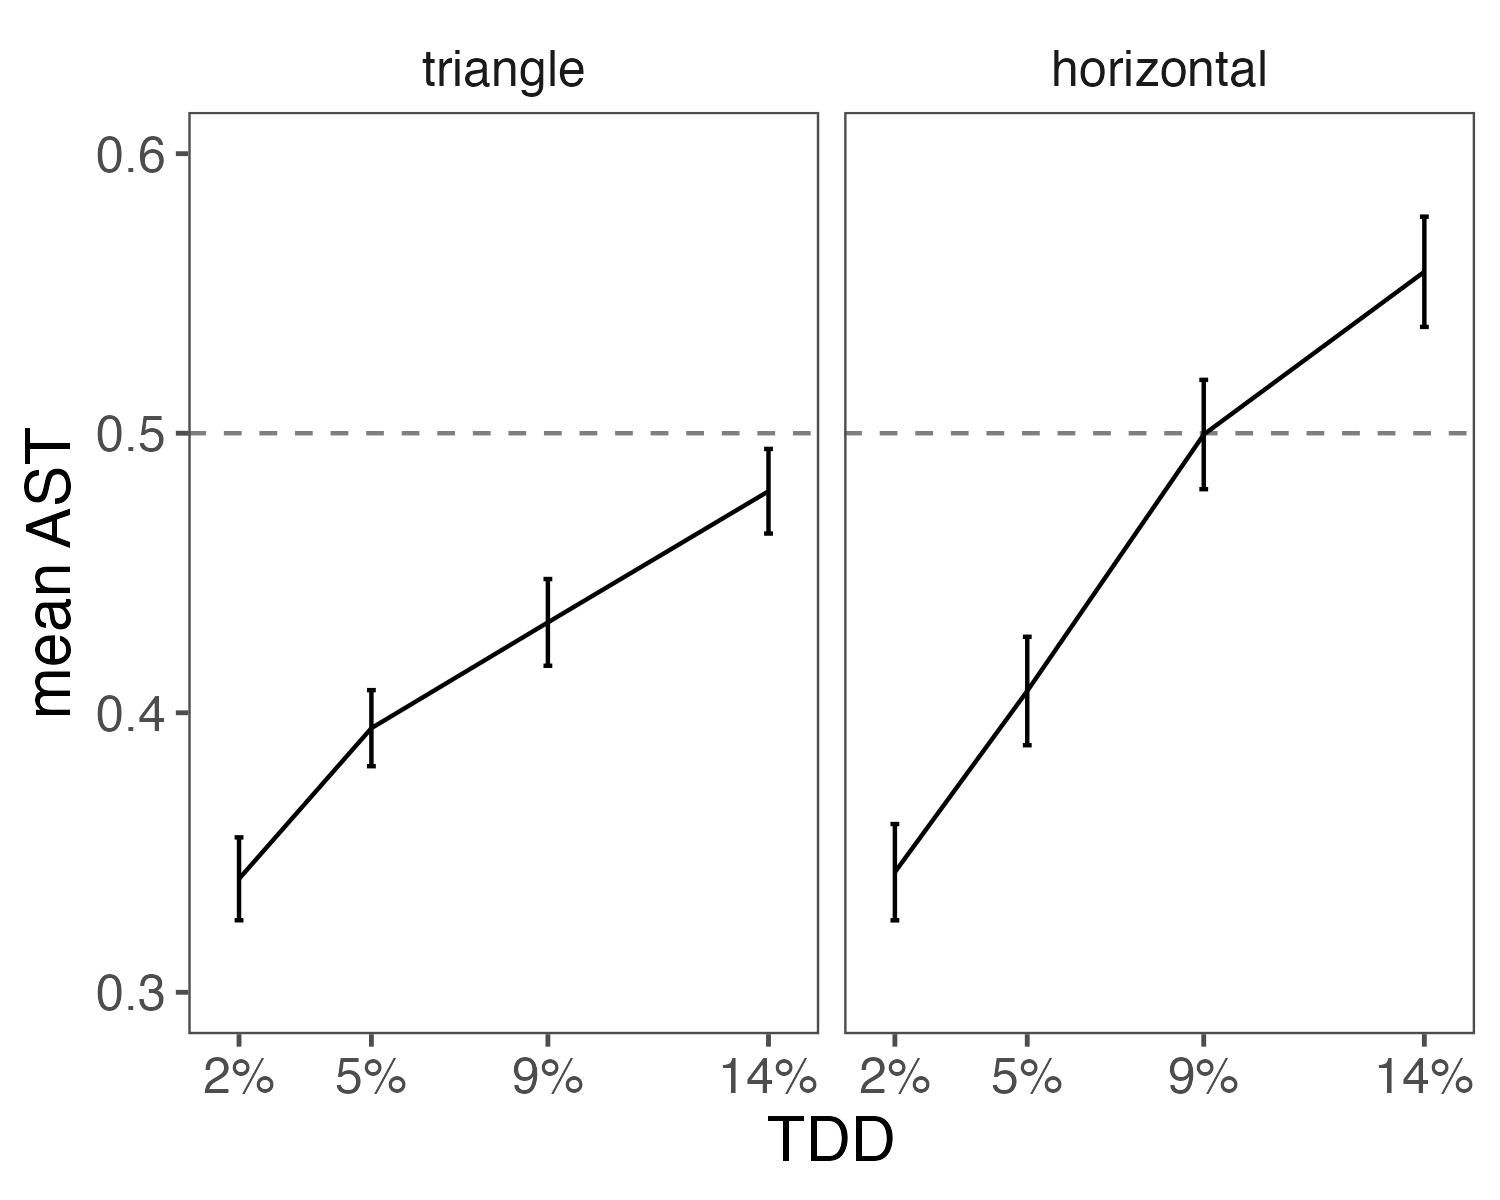
\includegraphics[width=100mm]{figures/choicePhase_mean_ast.jpeg}
   \caption{Mean AST values for each display condition and TDD level from Experiment 2. Error bars are $95\%$ CIs with the within-subjects correction from \textcite{cousineau2014error}.}
   \label{fig:e2_ast}
\end{figure}

\chapter{Bayesian Modeling of Price Data from Experiment 4}

I modeled the pricing data from Experiment 4 using a similar Thurstonian model to that of Experiment.

\section{Thurstonian Price Model}

I assumed that on each trial $i$, a vector of prices $\textbf{X}_{i}$ is drawn of a multivariate normal distribution:

\begin{align}
    \textbf{X}_{i}\sim \mathcal{N}(\boldsymbol{\mu}_{jk},\boldsymbol{\Sigma}_{k})
\end{align}

where $j$ is the product category (washing machines, laptops, televisions, microwave ovens) and $k$ is the trial type (attraction, repulsion). 

$\boldsymbol{\mu}_{jk}$ is the column vector:

\begin{align}
   \begin{pmatrix}
      \mu_{T_jk} \\
      \mu_{C_jk} \\
      \mu_{D_jk}
      \end{pmatrix}
   \label{eqn:mu_price}
\end{align}

and $\boldsymbol{\Sigma}_{k}$ is a $3\text{x}3$ positive semi-definite variance-covariance matrix:

\begin{align}
   \boldsymbol{\Sigma}_{k}=S\boldsymbol{\Omega}_{k}S
\end{align}

where $S$ is a diagonal matrix consisting of: 

\begin{align}
   \begin{pmatrix}
      \sigma_{T} & 0 & 0 \\
      0 & \sigma_{C} & 0 \\
      0 & 0 & \sigma_{D} 
   \end{pmatrix}
\end{align}

with $\sigma_{T}$, $\sigma_{C}$, $\sigma_{D}$ being the standard deviations for target, competitor, and decoy, respectively. $\boldsymbol{\Omega}_{k}$ is a correlation matrix:

\begin{align}
   \begin{pmatrix}
      1 & \rho_{TC_k} & \rho_{TD_k} \\
      \rho_{TC_k} & 1 & \rho_{CD_k} \\
      \rho_{TD_k} & \rho_{CD_k} & 1 
   \end{pmatrix}
\end{align}

with $\rho_{TD_1}$, for example, indicating the population-level correlation between target and decoy valuations in the attraction condition.

This model has relatively $24$ free parameters,relatively few compared to the several hundred from Experiment 2.

I had no a priori predictions about the size or even direction of the price differences here. Given this, I freely estimated all $\boldsymbol{\mu}$ parameters rather than estimate them through linear regression, as in Experiment 2.

Prior to model estimation, I z-scored all prices within subjects. 

\section{Prior Distributions on all Parameters}

\begin{itemize}
    \item $\boldsymbol{\mu}_{jk} \sim \mathcal{N}(0,1)$
    \item $\sigma_{T} \sim \text{Half-Cauchy}(0,2.5)$
    \item $\sigma_{C} \sim \text{Half-Cauchy}(0,2.5)$
    \item $\sigma_{D} \sim \text{Half-Cauchy}(0,2.5)$
    \item $\boldsymbol{\Omega_{k}} \sim \text{LKJCorr}(\eta=0.5)$
\end{itemize}

\section{Parameter Estimates}

For brevity, I omit $\boldsymbol{\mu}$ and $\sigma$ estimates and show only $\rho$ estimates below.
\begin{table}[ht]
    \centering
    \begin{tabular}{llrrrr}
        \toprule
        Trial Type & Parameter & \textit{M} & \textit{SD} & HDI lower & HDI upper \\
        \midrule
        \textbf{Attraction}  &  $\boldsymbol{\rho}_{TC}$     &    $.87$   &   $0.005$    &  $.86$     & $.88$     \\
                             &  $\boldsymbol{\rho}_{TD}$    &     $.87$   &   $0.005$    &  $.86$     & $.88$     \\
                             &  $\boldsymbol{\rho}_{CD}$    &     $.83$   &   $0.007$    &  $.81$     & $.84$     \\
        \textbf{Repulsion}   &  $\boldsymbol{\rho}_{TC}$     &    $.77$   &   $0.008$    &  $.75$     & $.79$     \\
                             &  $\boldsymbol{\rho}_{TD}$    &     $.87$   &   $0.005$    &  $.86$     & $.88$     \\
                             &  $\boldsymbol{\rho}_{CD}$    &     $.69$   &   $0.011$     &  $.67$     & $.72$     \\
        \bottomrule
    \end{tabular}
    \caption{$\rho$ Parameter estimates for Bayesian Hierarchical Thurstonian Model from Experiment 4 Pricing Data, including means, standard deviations, and $95\%$ Credible Intervals.}
    \label{tab:e4_rho_params}
\end{table}



%%
%% Beginning of back matter
\backmatter  %% <--- mandatory

%%
%% Idon't support endnotes

%%
%% A bibliography is required.
\interlinepenalty=10000  % prevent split bibliography entries
\printbibliography
\end{document}

%%% Local Variables: 
%%% mode: latex
%%% TeX-master: t
%%% End: 
